% !TeX program = xelatex
% ============================================================
%  李政道《数学物理方法》第一章 矢量与张量分析
%  扫描件重排试做：正文重新排版，插图全部用 TikZ/matplotlib 重绘
% ============================================================
\documentclass[11pt,a4paper,twoside,openright]{ctexbook}

\usepackage[margin=2.3cm]{geometry}
\usepackage{amsmath,amssymb,bm}
\usepackage{graphicx}
% 西文字体：Times New Roman（含西里尔字符，用于“Остроградский”等）
\setmainfont{Times New Roman}
\usepackage{tikz}
\usepackage{tikz-3dplot}
\tdplotsetmaincoords{70}{110}
\usetikzlibrary{arrows.meta,calc,patterns}
\usepackage{fancyhdr}
\usepackage{setspace}
\usepackage{enumitem}
\usepackage{multirow}

\newcommand{\ve}[1]{\bm{#1}}
\newcommand{\dd}{\,\mathrm{d}}

\ctexset{
  chapter = {
    name = {第,章},
    number = \chinese{chapter},
    format = {\centering\zihao{2}\heiti},
    beforeskip = 1.5em,
    afterskip  = 1.5em,
  },
  section = {
    name = {§,},
    number = \arabic{section},
    format = {\zihao{4}\heiti},
    beforeskip = 1.4em,
    afterskip  = 0.9em,
  },
}

% 页眉页脚
\pagestyle{fancy}
\fancyhf{}
\fancyhead[C]{\small\kaishu 数学物理方法}
\fancyfoot[C]{\small\thepage}
\renewcommand{\headrulewidth}{0.4pt}

\setstretch{1.18}

% 防止段首/段末孤行、显示公式前断页
\clubpenalty=10000
\widowpenalty=10000
\predisplaypenalty=10000

\makeatletter
\def\cleardoublepage{\clearpage\if@twoside\ifodd\c@page\else
\hbox{}\newpage\if@twocolumn\hbox{}\newpage\fi\fi\fi}
\makeatother

\begin{document}
% ---------------- 扉页 ----------------
\begin{titlepage}
\thispagestyle{empty}
\centering
\vspace*{3.5cm}
{\zihao{0}\heiti 数学物理方法}\\[2.2em]
{\zihao{3}\kaishu 李政道\quad 著}
\vfill
\end{titlepage}

% 扉页背面留空：保证正文第 1 页起于奇数页（正面）
\thispagestyle{empty}\mbox{}\clearpage

\frontmatter
\tableofcontents

\mainmatter

\chapter{矢量与张量分析}

% ============================================================
\section{矢量代数}

设 $(x_1,x_2,x_3)$ 为三维空间中的点 $P$ 在右旋笛卡尔坐标系中的坐标（图 1）。
这些坐标唯一地确定了点 $P$ 在空间中的位置：$P:(x_1,x_2,x_3)$。
设 $(x_1',x_2',x_3')$ 为同一个点在另一个右旋笛卡尔坐标系中的坐标，则该点在两个不同的坐标系中的坐标由下式联系：

\begin{figure}[htbp]
\centering
\begin{tikzpicture}[tdplot_main_coords, scale=2.4]
  \coordinate (O) at (0,0,0);
  % 实线：原坐标系
  \draw[->,thick] (O) -- (2.1,0,0) node[anchor=north east]{$x_1(x)$};
  \draw[->,thick] (O) -- (0,2.1,0) node[anchor=north west]{$x_2(y)$};
  \draw[->,thick] (O) -- (0,0,2.1) node[anchor=south]{$x_3(z)$};
  % 虚线：旋转后的新坐标系
  \draw[->,dashed,thick] (O) -- (1.85,0.62,0.5) node[anchor=north east]{$x_1'$};
  \draw[->,dashed,thick] (O) -- (-0.52,1.8,0.5) node[anchor=north west]{$x_2'$};
  \draw[->,dashed,thick] (O) -- (-0.2,-0.4,1.95) node[anchor=south]{$x_3'$};
  % 点 P
  \coordinate (P) at (1.5,1.0,1.2);
  \fill (P) circle (1.2pt);
  \node[above right] at (P) {$P(x_1,x_2,x_3)$};
\end{tikzpicture}
\par\vspace{2pt}
{\small 图 1.}
\end{figure}

\begin{equation}
\begin{aligned}
x_1' &= u_{11} x_1 + u_{12} x_2 + u_{13} x_3,\\
x_2' &= u_{21} x_1 + u_{22} x_2 + u_{23} x_3,\\
x_3' &= u_{31} x_1 + u_{32} x_2 + u_{33} x_3,
\end{aligned}
\tag{1.1}
\end{equation}

式(1.1)可更紧凑地写成：

\begin{equation*}
x_i' = \sum_{j=1}^{3} u_{ij} x_j \qquad (i = 1, 2, 3).
\end{equation*}

显然，此时数 $u_{ij}$ 需服从下面的关系式：

\begin{equation}
\sum_{i=1}^{3} u_{ij} u_{ik} = \sum_{i=1}^{3} u_{ji} u_{ki} = \delta_{jk}
= \begin{cases} 1, & \text{若 } j = k,\\ 0, & \text{若 } j \neq k. \end{cases}
\tag{1.1a}
\end{equation}

[$\delta_{jk}$ 称为克罗内克（Kronecker）符号]

于是，
\begin{equation*}
\begin{aligned}
u_{11}^{2} + u_{21}^{2} + u_{31}^{2} &= 1,\\
u_{11} u_{12} + u_{21} u_{22} + u_{31} u_{32} &= 0,
\end{aligned}
\end{equation*}

等等。

由三个数组成的有序集合 $(A_1, A_2, A_3)$，在轴的旋转下能作象上述的点 $P$ 的坐标 $(x_1, x_2, x_3)$ 一样的变换，即
$(A_1, A_2, A_3) \longrightarrow (A_1', A_2', A_3')$，则 $(A_1, A_2, A_3)$ 就叫做三维矢量，这里

\begin{equation}
A_i' = \sum_{j=1}^{3} u_{ij} A_j \qquad (i = 1, 2, 3),
\tag{1.2}
\end{equation}

而 $u_{ij}$ 为 $(x_1, x_2, x_3)$ 变到 $(x_1', x_2', x_3')$ 时由(1.1)所确定的系数。

今考虑几个矢量的例子。空间中的点 $P(x_1, x_2, x_3)$ 可与具有同样坐标的矢量 $\ve{r}$ 相对应，这个矢量常称为 $P$ 点的径矢。如果矢量 $\ve{r}$ 依赖于某个变量 $t$，则我们可构成 $(dx_1/dt, dx_2/dt, dx_3/dt)$，容易验证，它也是矢量。这个矢量常记为 $\ve{v} = d\ve{r}/dt$。类似地，可构造矢量 $\ve{a} = d\ve{v}/dt$。一般地，如有某个坐标依赖于参数的矢量，则通过对原先的矢量按坐标微商可构造一新的矢量。用这种方法得到的矢量，就称为所给矢量的导数。

两个矢量 $\ve{A}$ 和 $\ve{B}$，只要在同一个坐标系中的对应坐标完全相同，就认为是相等的。显然，如果两个矢量在某一个坐标系中的坐标完全相同，那么它们在另外任意一个系中也完全相同。

矢量
\begin{equation*}
\ve{A} + \ve{B} = (A_1 + B_1,\ A_2 + B_2,\ A_3 + B_3)
\end{equation*}

称为两矢量 $\ve{A} = (A_1, A_2, A_3)$ 和 $\ve{B} = (B_1, B_2, B_3)$ 的和。容易检验，用这种方法得到的量确是一矢量，且

\begin{equation*}
\ve{A} + \ve{B} = \ve{B} + \ve{A}.
\end{equation*}

\textbf{例 1}\quad 矢量相等的几何解释。设 $\ve{A}$ 为某个矢量，而 $\ve{r}_P$，$\ve{r}_Q$ 分别为点 $P$ 和 $Q$ 的径矢。选取这样一些点，使得

\begin{equation*}
A_1 = x_{1P} - x_{1Q}, \qquad A_2 = x_{2P} - x_{2Q}, \qquad A_3 = x_{3P} - x_{3Q},
\end{equation*}

于是 $\ve{A} = \ve{r}_{PQ}$（图 3）。由此，任一矢量都可对应于某个线段；换句话说，所有矢量在空间中都有方向和大小这种特性。

\begin{figure}[htbp]
\centering
\begin{tikzpicture}[tdplot_main_coords, scale=2.2]
  \coordinate (O) at (0,0,0);
  % 坐标轴
  \draw[->,thick] (O) -- (2.1,0,0) node[anchor=north east]{$x_1$};
  \draw[->,thick] (O) -- (0,2.1,0) node[anchor=north west]{$x_2$};
  \draw[->,thick] (O) -- (0,0,2.1) node[anchor=south]{$x_3$};
  % 位置矢量 r → P
  \coordinate (P) at (1.5,1.0,1.2);
  \draw[->,very thick] (O) -- (P) node[midway,above]{$\ve{r}$};
  \fill (P) circle (1.2pt);
  \node[above] at (P) {$P(x_1,x_2,x_3)$};
\end{tikzpicture}
\par\vspace{2pt}
{\small 图 2.}
\end{figure}

\begin{figure}[htbp]
\centering
\begin{tikzpicture}[tdplot_main_coords, scale=2.2]
  \coordinate (O) at (0,0,0);
  % 坐标轴
  \draw[->,thick] (O) -- (2.1,0,0) node[anchor=north east]{$x_1$};
  \draw[->,thick] (O) -- (0,2.1,0) node[anchor=north west]{$x_2$};
  \draw[->,thick] (O) -- (0,0,2.1) node[anchor=south]{$x_3$};
  % 三角形 O-P-Q（原图三角形边无箭头；r_P 比 r_Q 长）
  \coordinate (P) at (1.5,1.1,1.7);
  \coordinate (Q) at (1.6,1.3,0.3);
  \draw[very thick] (O) -- (P) node[midway,below left]{$\ve{r}_P$};
  \draw[very thick] (O) -- (Q) node[midway,below right]{$\ve{r}_Q$};
  \draw[very thick] (P) -- (Q) node[midway,above right]{$\ve{r}_{PQ}$};
  \fill (O) circle (1.2pt);
  \fill (P) circle (1.2pt) node[above left]{$P$};
  \fill (Q) circle (1.2pt) node[below right]{$Q$};
\end{tikzpicture}
\par\vspace{2pt}
{\small 图 3.}
\end{figure}

数
\begin{equation*}
\ve{A} \cdot \ve{B} = \sum_{i=1}^{3} A_i B_i
\end{equation*}

称为两矢量 $\ve{A}$ 和 $\ve{B}$ 的数量积 $\ve{A} \cdot \ve{B}$。数量积是关于坐标系旋转的不变量。事实上，利用公式(1.1)得

\begin{equation*}
\begin{aligned}
\sum_{i=1}^{3} A_i' B_i'
&= \sum_{i,j,k} u_{ij} A_j\, u_{ik} B_k
 = \sum_{j,k} \left(\sum_{i=1}^{3} u_{ij} u_{ik}\right) A_j B_k\\
&= \sum_{j,k} \delta_{jk} A_j B_k = \sum_{j=1}^{3} A_j B_j.
\end{aligned}
\end{equation*}

在坐标系作转动时不变的量，叫做标量。于是 $\ve{A} \cdot \ve{B}$ 是标量。显然，$\ve{A} \cdot \ve{A} = \sum_{i=1}^{3} A_i^{2}$。数 $(\ve{A} \cdot \ve{A})^{1/2}$ 称为矢量 $\ve{A}$ 的模（或长度），并记之为 $|\ve{A}|$。特别是，如果 $\ve{A} = \ve{r}$，则

\begin{equation*}
|\ve{A}| = |\ve{r}| = \sqrt{x_1^{2} + x_2^{2} + x_3^{2}}.
\end{equation*}

今选取坐标系，使得轴 $x_1$ 顺着矢量 $\ve{A}$ 的方向，而矢量 $\ve{B}$ 则在平面 $x_1 x_2$ 内（图 4），于是

\begin{figure}[htbp]
\centering
\begin{tikzpicture}[scale=1.8]
  % x1 轴 = 矢量 A（同一条黑色带箭头线段）
  \draw[->,very thick] (-0.2,0) -- (3.6,0);
  \node[right] at (3.65,0) {$x_1$};
  \node[below] at (1.85,-0.14) {$A$};
  % x2 轴
  \draw[->] (0,-0.2) -- (0,2.5) node[above]{$x_2$};
  % 矢量 B（黑色带箭头）
  \draw[->,very thick] (0,0) -- (2.6,1.95) node[midway,above left]{$B$};
  % θ 弧（较大，离原点较远）
  \draw (1.12,0) arc[start angle=0, end angle=36.9, radius=1.12];
  \node at (1.52,0.42) {$\theta$};
\end{tikzpicture}
\par\vspace{2pt}
{\small 图 4.}
\end{figure}

\begin{equation*}
\begin{aligned}
\ve{A} &= (A, 0, 0),\\
\ve{B} &= (B \cos\theta,\ B \sin\theta,\ 0),\\
\ve{A} \cdot \ve{B} &= |\ve{A}|\,|\ve{B}| \cos\theta,
\end{aligned}
\end{equation*}

这里 $\theta$ 是矢量 $\ve{A}$ 和 $\ve{B}$ 之间的夹角。因 $\ve{A} \cdot \ve{B}$ 是标量，故这个等式在任意坐标系中都仍适合。特别地，如果 $\ve{A} \cdot \ve{B} = 0$，且 $\ve{A}$ 和 $\ve{B}$ 都不为零，则矢量 $\ve{A}$ 和 $\ve{B}$ 垂直。

\textbf{例 2}\quad 能量守恒。由牛顿第二定律

\begin{equation}
\ve{F} = m \ve{a} = m \frac{d\ve{v}}{dt},
\tag{1.3}
\end{equation}

这里 $m$ 为物体质量，$\ve{F}$ 为作用于该物体上的力，$\ve{v}$ 为速度。
在等式(1.3)两边点乘 $\ve{v}$，则得

\begin{equation*}
\begin{aligned}
\ve{F} \cdot \ve{v}
&= m \frac{d\ve{v}}{dt} \cdot \ve{v} = \sum_{i=1}^{3} m \frac{dv_i}{dt} v_i\\
&= \sum_{i=1}^{3} m \frac{d}{dt} \left(\frac{v_i^{2}}{2}\right) = \frac{d}{dt} \left(\frac{m v^{2}}{2}\right),
\end{aligned}
\end{equation*}

即
\begin{equation*}
\ve{F} \cdot \ve{v} = \frac{d}{dt} \left(\frac{m v^{2}}{2}\right)
\end{equation*}

这里 $v$ 为矢量 $\ve{v}$ 的模。特别，如果 $\ve{F} = 0$，则

\begin{equation*}
\frac{d}{dt} \left(\frac{m v^{2}}{2}\right) = 0, \qquad \text{即} \quad \frac{m v^{2}}{2} = \mathrm{const}.
\end{equation*}

这是能量守恒定律的一种形式。

\textbf{定理 1.1}\quad 假定有一个法则，使在每一坐标系中都能给出三个数 $(A_1, A_2, A_3)$，如果此法则对所有矢量 $\ve{B} = (B_1, B_2, B_3)$，都能使量 $\sum_{i=1}^{3} A_i B_i$ 为标量，则量 $\ve{A} = (A_1, A_2, A_3)$ 为矢量。

\textbf{证明}\quad 在坐标系转动下，矢量 $\ve{B}$ 的坐标按公式(1.2)变成：

\begin{equation*}
B_i' = \sum_{j=1}^{3} u_{ij} B_j \qquad (i = 1, 2, 3).
\end{equation*}

设在转动时，$(A_1, A_2, A_3)$ 变成 $(A_1', A_2', A_3')$。

我们需证
\begin{equation*}
A_i' = \sum_{j=1}^{3} u_{ij} A_j \qquad (i = 1, 2, 3).
\end{equation*}

但由假设
\begin{equation*}
\sum_{i=1}^{3} A_i' B_i' = \sum_{i=1}^{3} A_i B_i,
\end{equation*}

所以
\begin{equation*}
\sum_{i=1}^{3} A_i B_i = \sum_{i=1}^{3} A_i' \sum_{j=1}^{3} u_{ij} B_j = \sum_{j=1}^{3} \left(\sum_{i=1}^{3} u_{ij} A_i'\right) B_j.
\end{equation*}

因矢量 $\ve{B}$ 是任意给定的，故

\begin{equation}
A_j = \sum_{k=1}^{3} u_{kj} A_k' \qquad (j = 1, 2, 3).
\tag{1.4}
\end{equation}

将(1.4)乘以 $u_{ij}$，且对 $j$ 求和，考虑到(1.2)，就得

\begin{equation*}
\begin{aligned}
\sum_{j=1}^{3} u_{ij} A_j
&= \sum_{j=1}^{3} \sum_{k=1}^{3} u_{ij} u_{kj} A_k' = \sum_{k=1}^{3} A_k' \sum_{j=1}^{3} u_{ij} u_{kj}\\
&= \sum_{k=1}^{3} \delta_{ik} A_k' = A_i' \qquad (i = 1, 2, 3),
\end{aligned}
\end{equation*}

这就是所要证明的。

现考虑某个直角坐标系。设 $\ve{i} = (1, 0, 0)$，$\ve{j} = (0, 1, 0)$，$\ve{k} = (0, 0, 1)$ 为此坐标系中的三个单位矢量。则

\begin{equation*}
\begin{aligned}
\ve{i} \cdot \ve{i} = \ve{j} \cdot \ve{j} = \ve{k} \cdot \ve{k} &= 1,\\
\ve{i} \cdot \ve{j} = \ve{j} \cdot \ve{k} = \ve{k} \cdot \ve{i} &= 0
\end{aligned}
\end{equation*}

这些关系显示了单位矢量之间是相互垂直的。在这个坐标系中，矢量 $\ve{A} = (A_1, A_2, A_3)$ 可表示为

\begin{equation}
\ve{A} = A_1 \ve{i} + A_2 \ve{j} + A_3 \ve{k}.
\tag{1.5}
\end{equation}

将坐标轴旋转。原坐标系中的单位矢量在新坐标系中的坐标为

\begin{equation*}
\begin{aligned}
\ve{i} &: (u_{11}, u_{21}, u_{31}),\\
\ve{j} &: (u_{12}, u_{22}, u_{32}),\\
\ve{k} &: (u_{13}, u_{23}, u_{33}).
\end{aligned}
\end{equation*}

假定 $\ve{i}' = (1, 0, 0)$，$\ve{j}' = (0, 1, 0)$，$\ve{k}' = (0, 0, 1)$ 是新坐标系 $(x_1', x_2', x_3')$ 中的单位矢量。则由(1.2)和(1.5)式

\begin{equation}
\begin{aligned}
\ve{i} &= u_{11} \ve{i}' + u_{21} \ve{j}' + u_{31} \ve{k}',\\
\ve{j} &= u_{12} \ve{i}' + u_{22} \ve{j}' + u_{32} \ve{k}',\\
\ve{k} &= u_{13} \ve{i}' + u_{23} \ve{j}' + u_{33} \ve{k}'.
\end{aligned}
\tag{1.6}
\end{equation}

显然 $\ve{i}' \cdot \ve{i}' = 1$，$\ve{i}' \cdot \ve{j}' = 0$ 等等。因此

\begin{equation*}
\begin{aligned}
\ve{i} \cdot \ve{i} &= u_{11}^{2} + u_{21}^{2} + u_{31}^{2} = 1,\\
\ve{i} \cdot \ve{j} &= u_{11} u_{12} + u_{21} u_{22} + u_{31} u_{32} = 0.
\end{aligned}
\end{equation*}

我们又得到了(1.1)，并顺便说明了它们的起源。注意，由前面的结论从(1.4)式可推出，新坐标系中的单位矢量可用下面的方式由原坐标系中的单位矢量表出：

\begin{equation}
\begin{aligned}
\ve{i}' &= u_{11} \ve{i} + u_{12} \ve{j} + u_{13} \ve{k},\\
\ve{j}' &= u_{21} \ve{i} + u_{22} \ve{j} + u_{23} \ve{k},\\
\ve{k}' &= u_{31} \ve{i} + u_{32} \ve{j} + u_{33} \ve{k}.
\end{aligned}
\tag{1.7}
\end{equation}

有两个矢量 $\ve{A}$ 和 $\ve{B}$，若置

\begin{equation*}
\begin{aligned}
\ve{A} \times \ve{B} &= (A_2 B_3 - A_3 B_2,\ A_3 B_1 - A_1 B_3,\\
&\qquad\quad A_1 B_2 - A_2 B_1),
\end{aligned}
\end{equation*}

则可构造第三个矢量。下面将验证，$\ve{A} \times \ve{B}$ 确是矢量。为此，利用定理 1.1。即要证明，对所有矢量 $\ve{C}$，$(\ve{A} \times \ve{B}) \cdot \ve{C}$ 是标量。容易验证，

\begin{equation}
(\ve{A} \times \ve{B}) \cdot \ve{C} =
\begin{vmatrix}
A_1 & A_2 & A_3\\
B_1 & B_2 & B_3\\
C_1 & C_2 & C_3
\end{vmatrix}
\tag{1.8}
\end{equation}

位于(1.8)式右边的行列式，等于由矢量 $\ve{A}$，$\ve{B}$ 和 $\ve{C}$ 所构成的平行六面体的体积。显然，体积关于旋转是不变的。而这对

\begin{figure}[htbp]
\centering
\begin{tikzpicture}[scale=1.7]
  \coordinate (O) at (0,0);
  % A（黑色线段，无箭头，沿 i 方向=左下）
  \draw[very thick] (O) -- (-2.3,-1.15) node[midway,below left]{$A$};
  % B（黑色线段，无箭头，沿 j 方向=右）
  \draw[very thick] (O) -- (2.55,0) node[midway,below]{$B$};
  % A×B（黑色带箭头，沿 k 方向=上）
  \draw[->,very thick] (O) -- (0,2.45) node[midway,left]{$A \times B$};
  % 单位矢量 i、j、k 靠近原点
  \node[below left] at (-0.9,-0.45) {$i$};
  \node[below] at (0.8,0.2) {$j$};
  \node[above] at (0.18,0.8) {$k$};
  % θ 大弧（从 A 到 B，穿越 j 轴下方）
  \draw[->] (-0.95,-0.47) arc[start angle=-153.4, end angle=-12, radius=1.0];
  \node at (0.4,-0.95) {$\theta$};
  \fill (O) circle (1.2pt);
\end{tikzpicture}
\par\vspace{2pt}
{\small 图 5.}
\end{figure}

任一矢量 $\ve{C}$ 都是正确的，故由定理(1.1)知，$\ve{A} \times \ve{B}$ 确实是矢量。这个矢量称为矢量 $\ve{A}$ 和 $\ve{B}$ 的矢量积。

现在来确定矢量 $\ve{A} \times \ve{B}$ 的方向和大小。为此目的，我们选取坐标轴，使得矢量 $\ve{A}$ 顺着 $\ve{i}$ 的方向，而矢量 $\ve{B}$ 位于 $ij$ 平面内。于是在此坐标系内

\begin{equation*}
\ve{A} = (A, 0, 0),
\end{equation*}

\begin{equation*}
\ve{B} = (B \cos\theta,\ B \sin\theta,\ 0),
\end{equation*}

\begin{equation*}
\ve{A} \times \ve{B} = (0,\ 0,\ |\ve{A}|\,|\ve{B}| \sin\theta),
\end{equation*}

$\theta = \angle(\ve{A}, \ve{B})$ 为 $\ve{A}$ 和 $\ve{B}$ 之间的夹角。

因此
\begin{equation*}
|\ve{A} \times \ve{B}| = |\ve{A}|\,|\ve{B}|\,|\sin\theta|,
\end{equation*}

矢量 $\ve{A}$ 和 $\ve{B}$ 与矢量 $\ve{A} \times \ve{B}$ 垂直。矢量 $\ve{A}$，$\ve{B}$ 和 $\ve{A} \times \ve{B}$ 构成右旋三矢量。易知，如果矢量 $\ve{A}$ 与 $\ve{B}$ 平行，则 $\ve{A} \times \ve{B} = 0$；而在一般情形，矢量 $\ve{A} \times \ve{B}$ 的大小等于由矢量 $\ve{A}$ 和 $\ve{B}$ 所构成的平行四边形的面积。特别地，$\ve{i} \times \ve{i} = 0$ 等等，以及

\begin{equation*}
\ve{i} \times \ve{j} = \ve{k}, \qquad \ve{k} \times \ve{j} = -\ve{i}, \qquad \ve{j} \times \ve{k} = \ve{i}.
\end{equation*}

\textbf{例 3}\quad 有心力场内的动量矩守恒定律。设 $\ve{r} = \ve{r}(t)$ 为动点的径矢。如用 $\ve{F}$ 表示作用力，则由牛顿第二定律，$\ve{F} = m \ddot{\ve{r}}$（在矢量上面的点，今后都表示对时间 $t$ 的微商）。

如果矢量 $\ve{r}$ 和力 $\ve{F}$ 在任一时刻 $t$ 都互相平行，则力 $\ve{F}$ 称为有心力。重力，点电荷场内的静电力等都可以作为有心力的例子。要证明的是，在有心力的情形，矢量 $\ve{p} = m\ve{v}$（$\ve{p}$ 为动量，$m$ 为物体的质量，$\ve{v}$ 为物体的速度）常位于某个固定的平面内。今证明这个结论。

动点的径矢与其动量的矢量积叫做动量矩：

\begin{equation}
\ve{L} = \ve{r} \times \ve{p}.
\tag{1.9}
\end{equation}

(1.9)两边对 $t$ 微商，得

\begin{equation*}
\dot{\ve{L}} = \dot{\ve{r}} \times \ve{p} + \ve{r} \times \dot{\ve{p}}.
\end{equation*}

因动量矢与速度矢平行，故

\begin{equation*}
\dot{\ve{r}} \times \ve{p} = 0.
\end{equation*}

而由牛顿第二定律，$\dot{\ve{p}} = \ve{F}$；再由有心力的定义，便推得

\begin{equation*}
\ve{r} \times \dot{\ve{p}} = 0.
\end{equation*}

因此，
\begin{equation*}
\dot{\ve{L}} = 0 \qquad \text{或} \qquad \ve{L} = \mathrm{const}.
\end{equation*}

即在有心力的情形，动量矩是运动的积分（大小和方向守恒）。由(1.9)可看出，$\ve{p}$ 总位于与 $\ve{L}$ 垂直、在空间中位置固定的平面内。这就证明了我们的结论。

\textbf{例 4}\quad 无限小角度转动。考虑绕 $z$ 轴旋转。设 $\ve{r} = \ve{r}(t)$ 为质点在时刻 $t$ 的径矢，$\delta t$ 为无限小时间间隔。在 $\delta t$ 时间内，质点的径矢绕 $z$ 轴转过了小角度 $\delta\varphi$。因 $\delta\varphi \ll 1$，故下列关系式成立：

\begin{equation}
\cos\delta\varphi \approx 1 - \frac{(\delta\varphi)^{2}}{2}, \qquad
\sin\delta\varphi \approx \delta\varphi - \frac{(\delta\varphi)^{3}}{3!}.
\tag{1.10}
\end{equation}

利用(1.10)，可求出质点在转过 $\delta\varphi$ 角后（时间 $\delta t$ 后）的坐标：

\begin{equation}
\begin{aligned}
z(\delta t) &= z(0),\\
x(\delta t) &= x(0) - y(0)\,\delta\varphi + O(\delta\varphi^{2}),\\
y(\delta t) &= x(0)\,\delta\varphi + y(0) + O(\delta\varphi^{2}).
\end{aligned}
\tag{1.11}
\end{equation}

这里 $O(\delta\varphi^{2})$ 是 $(\delta\varphi)^{2}$ 的同级无穷小量。另一方面，当 $\delta t \to 0$ 时，在原点邻域内将 $x(t)$ 和 $y(t)$ 展开成泰勒（Taylor）级数，并限取前二项，则有

\begin{equation}
\begin{aligned}
x(\delta t) &= x(0) + \dot{x}\,\delta t,\\
y(\delta t) &= y(0) + \dot{y}\,\delta t.
\end{aligned}
\tag{1.12}
\end{equation}

比较(1.11)和(1.12)，就得

\begin{equation*}
\begin{aligned}
\dot{x}(t) &= -\left(\frac{\delta\varphi}{\delta t}\right) y,\\
\dot{y}(t) &= \left(\frac{\delta\varphi}{\delta t}\right) x,\\
\dot{z}(t) &= 0.
\end{aligned}
\end{equation*}

今用 $\ve{\omega}$ 记方向平行于旋转轴，大小等于 $\delta\varphi / \delta t$ 的矢量。在我们的情形，

\begin{equation*}
\ve{\omega} = \left(0,\ 0,\ \frac{\delta\varphi}{\delta t}\right)
\end{equation*}

因此
\begin{equation}
\dot{\ve{r}} = \ve{\omega} \times \ve{r}.
\tag{1.13}
\end{equation}

在(1.13)中所有的量都是矢量。因此，我们可以断言，这个等式在任一坐标系中都是正确的。

在 $\ve{\omega}$ 为常量的情形，加速度 $\ve{a}$ 可用下式计算：

\begin{equation*}
\begin{aligned}
\ve{a} \equiv \ddot{\ve{r}} &= \frac{d}{dt}(\ve{\omega} \times \ve{r}) = \ve{\omega} \times \dot{\ve{r}}\\
&= \ve{\omega} \times (\ve{\omega} \times \ve{r}),
\end{aligned}
\end{equation*}

如果矢量 $\ve{\omega}$ 与矢量 $\ve{r}$ 垂直，则

\begin{equation*}
|\ve{a}| = |\ve{\omega}|\,|\ve{\omega} \times \ve{r}| = |\ve{\omega}|^{2}\,|\ve{r}|,
\end{equation*}

且 $\ve{a}$ 与矢量 $\ve{r}$ 方向相反。而

\begin{equation*}
|\ve{v}| = |\ve{\omega} \times \ve{r}| = |\ve{\omega}|\,|\ve{r}|,
\end{equation*}

所以
\begin{equation*}
\ve{a} = -|\ve{\omega}|^{2}\,\ve{r} = -\frac{|\ve{v}|^{2}}{|\ve{r}|^{2}}\,\ve{r}.
\end{equation*}

现研究空间质点沿某个轨道运动的一般情形。假定

\begin{equation*}
\ve{\tau} = \frac{\ve{v}}{|\ve{v}|},
\end{equation*}

则 $\ve{\tau}$ 为与质点轨道相切的单位矢量（图 6）。将上式对 $t$ 微分，得

\begin{figure}[htbp]
\centering
\begin{tikzpicture}[tdplot_main_coords, scale=2.1]
  % 坐标轴
  \draw[->,thick] (0,0,0) -- (2.1,0,0) node[anchor=north east]{$x_1$};
  \draw[->,thick] (0,0,0) -- (0,2.1,0) node[anchor=north west]{$x_2$};
  \draw[->,thick] (0,0,0) -- (0,0,2.0) node[anchor=south]{$x_3$};
  % 空间曲线 r(t)（拱形，从左下向右上延伸）
  \draw[very thick] plot[smooth] coordinates
    {(0.55,0.35,0.08) (1.0,0.95,0.3) (1.5,1.65,0.55) (1.9,2.35,0.85) (2.1,3.0,1.15)};
  % 位置矢量 r（原点 → 曲线上的点 P）
  \coordinate (P) at (1.5,1.65,0.55);
  \draw[->,thick] (0,0,0) -- (P) node[midway,below right]{$\ve{r}$};
  \fill (P) circle (1.2pt);
  % Frenet 标架：τ 沿切线（右略上），N 竖直向上，b 右上方（原书为黑白）
  \draw[->,very thick] (P) -- +(0.35,0.65,0.35) node[above]{$\ve{\tau}$};
  \draw[->,very thick] (P) -- +(0,0,0.95) node[above]{$\ve{N}$};
  \draw[->,very thick] (P) -- +(0.25,0.5,0.6) node[right]{$\ve{b}$};
\end{tikzpicture}
\par\vspace{2pt}
{\small 图 6.}
\end{figure}

\begin{equation*}
\ve{a} \equiv \dot{\ve{v}} = \frac{d|\ve{v}|}{dt}\,\ve{\tau} + |\ve{v}|\, \dot{\ve{\tau}}.
\end{equation*}

但由等式 $\ve{\tau} \cdot \ve{\tau} = 1$ 推出

\begin{equation*}
\dot{\ve{\tau}} \cdot \ve{\tau} = 0,
\end{equation*}

即矢量 $\ve{\tau}$ 与 $\dot{\ve{\tau}}$ 垂直。这样一来，加速度 $\ve{a}$ 可分解为切向加速度和与它相垂直的法向加速度。引进单位矢量

\begin{equation}
\ve{N} = \frac{\dot{\ve{\tau}}}{|\dot{\ve{\tau}}|},
\tag{1.14}
\end{equation}

它与 $\ve{\tau}$ 垂直。并称它为曲线 $\ve{r} = \ve{r}(t)$ 的法矢量。如果 $S$ 为曲线从任一固定点量起的弧长，则下面等式成立：

\begin{equation}
\dot{\ve{\tau}} = \dot{S}\,\frac{d\ve{\tau}}{dS} = |\ve{v}|\,\frac{d\ve{\tau}}{dS}, \qquad (\dot{S} = |\ve{v}|)
\tag{1.15}
\end{equation}

由此
\begin{equation*}
\ve{N} = \frac{\dot{\ve{\tau}}}{|\ve{v}|\left|\frac{d\ve{\tau}}{dS}\right|},
\end{equation*}

\begin{equation*}
\ve{a} = \ve{N}\,|\ve{v}|^{2}\left|\frac{d\ve{\tau}}{dS}\right| + \ve{\tau}\,|\dot{\ve{v}}|.
\end{equation*}

量
\begin{equation*}
R \equiv \frac{1}{\left|\frac{d\ve{\tau}}{dS}\right|}
\end{equation*}

称为曲线的曲率半径。$R = \infty$（即 $d\ve{\tau}/dS = 0$）时的点称为曲线的拐点。

现在我们能写

\begin{equation*}
\ve{a} = \ve{N}\,\frac{|\ve{v}|^{2}}{R} + \ve{\tau}\,|\dot{\ve{v}}|.
\end{equation*}

对于匀速圆周运动，这个公式便成为

\begin{equation*}
\ve{a} = -\frac{|\ve{v}|^{2}}{|\ve{r}|^{2}}\,\ve{r}.
\end{equation*}

矢量 $\ve{N}$ 的方向用矢量 $d\ve{\tau}/dS$ 的方向确定。

根据定义，速度矢量 $\ve{v}$ 和加速度矢量 $\ve{a}$ 一样，位于由法向和切向单位矢量所构成的平面内。

因法向和切向单位矢量平面在空间中的位置随着时间而可能改变，于是速度和加速度给定了的质点轨道在一定程度上仍是自由的。我们将取曲线的挠率作为合适的参量。下面在计算自由加速度时，将利用挠率的概念。

法矢量和切矢量的矢量积 $\ve{b}$，叫做副法矢量：

\begin{equation}
\ve{b} = \ve{\tau} \times \ve{N}.
\tag{1.16}
\end{equation}

例如，若质点在平面内运动，则副法矢量为常量。

今用公式
\begin{equation*}
T \equiv \left|\frac{d\ve{b}}{dS}\right|
\end{equation*}

定义曲线的挠率 $T$。由图 7 看出，$|d\ve{b}| = d\theta$，因为 $|\ve{b}| = 1$，$\ve{b}$ 与矢量 $\ve{\tau}$ 与 $\ve{N}$ 的平面垂直以及 $d\theta$ 是这个平面的转动角。

\begin{figure}[htbp]
\centering
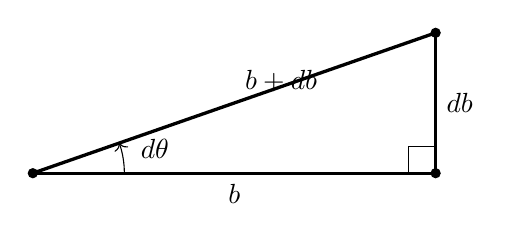
\begin{tikzpicture}[scale=1.55]
  % 直角三角形：底边 b、右边 db、斜边 b+db（说明 |db| = dθ）
  \coordinate (A) at (0,0);
  \coordinate (B) at (3.3,0);
  \coordinate (C) at (3.3,1.15);
  \draw[very thick] (A) -- (B) node[midway,below]{$b$};
  \draw[very thick] (B) -- (C) node[midway,right]{$db$};
  \draw[very thick] (A) -- (C) node[midway,above right]{$b+db$};
  \fill (A) circle (1.2pt) (B) circle (1.2pt) (C) circle (1.2pt);
  % dθ 弧（左下角）
  \draw[->] (0.75,0) arc[start angle=0, end angle=19.2, radius=0.75];
  \node at (1.0,0.2) {$d\theta$};
  % 直角标记
  \draw (3.08,0) -- (3.08,0.22) -- (3.3,0.22);
\end{tikzpicture}
\par\vspace{2pt}
{\small 图 7.}
\end{figure}

有时我们还用下面的记号：

\begin{equation*}
C_1 = \frac{1}{R} \text{——曲线曲率（第一曲率）},
\end{equation*}

\begin{equation*}
C_2 = \left|\frac{d\ve{b}}{dS}\right| \text{——曲线挠率（第二曲率）}, \qquad
C = \sqrt{C_1^{2} + C_2^{2}} \text{——全曲率}.
\end{equation*}

微分(1.16)，得

\begin{equation*}
\dot{\ve{b}} = \dot{\ve{\tau}} \times \ve{N} + \ve{\tau} \times \dot{\ve{N}}.
\end{equation*}

但矢量 $\dot{\ve{\tau}}$ 平行于矢量 $\ve{N}$，因此，$\dot{\ve{\tau}} \times \ve{N} = 0$，所以

\begin{equation*}
\dot{\ve{b}} = \ve{\tau} \times \dot{\ve{N}}.
\end{equation*}

因 $\ve{b} \cdot \ve{b} = 1$，故 $\dot{\ve{b}} \cdot \ve{b} = 0$。这样矢量 $\dot{\ve{b}}$ 就和矢量 $\ve{b}$ 与 $\ve{\tau}$ 垂直，从而就知矢量 $\dot{\ve{b}}$ 和矢量 $\ve{N}$ 平行。

\textbf{定理 1.2}\quad 全曲率等于矢量 $d\ve{N}/dS$ 的模：

\begin{equation*}
C = \left|\frac{d\ve{N}}{dS}\right|.
\end{equation*}

\textbf{证明}\quad 在矢量积(1.16)内进行循环交换，就给出

\begin{equation}
\ve{N} = \ve{b} \times \ve{\tau}.
\tag{1.17}
\end{equation}

将(1.17)对 $S$ 微分，得

\begin{equation}
\frac{d\ve{N}}{dS} = \frac{d\ve{b}}{dS} \times \ve{\tau} + \ve{b} \times \frac{d\ve{\tau}}{dS}.
\tag{1.18}
\end{equation}

其次，由(1.15)和(1.14)容易看出，矢量 $\ve{N}$ 平行于 $d\ve{\tau}/dS$，所以矢量 $\ve{b} \times d\ve{\tau}/dS$ 与矢量 $\dot{\ve{\tau}}$ 垂直。现在很明显，矢量 $\ve{b} \times d\ve{\tau}/dS$ 平行于矢量 $\ve{\tau}$。此外，

\begin{equation}
\left|\ve{b} \times \frac{d\ve{\tau}}{dS}\right| = \left|\frac{d\ve{\tau}}{dS}\right| = C_1;
\tag{1.19}
\end{equation}

类似地可证，矢量 $(d\ve{b}/dS) \times \ve{\tau}$ 平行于 $\ve{b}$，而

\begin{equation}
\left|\frac{d\ve{b}}{dS} \times \ve{\tau}\right| = \left|\frac{d\ve{b}}{dS}\right| = C_2.
\tag{1.20}
\end{equation}

在等式(1.18)右边部分内是两个互相垂直的矢量。因此，由(1.19)和(1.20)即可推得定理的结论：

\begin{equation*}
C = \left|\frac{d\ve{N}}{dS}\right|.
\end{equation*}

% ============================================================
\section{张量代数}

许多从物理观点来看非常重要的量，既不是矢量也不是标量。作为例子，我们引进与物体转动惯量有关的量 $x_i x_j$。当物体转动时，此量按下式变换：

\begin{equation*}
x_i' x_j' = \sum_{k,l=1}^{3} u_{ik} u_{jl}\, x_k x_l.
\end{equation*}

引入张量的概念。如果每个笛卡尔坐标系都有 $3^{n}$ 个数 $T_{i_1 i_2 \cdots i_n}$（这里 $i_1, i_2, \cdots, i_n$ 各自跑过值 $1, 2, 3$）与之对应，且这些数当由一个笛卡尔坐标系变到另一个时按规律

\begin{equation}
T_{i_1 i_2 \cdots i_n}' = \sum_{j_1, j_2, \cdots, j_n = 1}^{3} u_{i_1 j_1} u_{i_2 j_2} \cdots u_{i_n j_n}\, T_{j_1 j_2 \cdots j_n}
\tag{1.21}
\end{equation}

变换，则这 $3^{n}$ 个数全体就称为三维空间中的一个 $n$ 阶张量，这里 $u_{ij}$ 是过渡到新坐标系的矩阵。现考虑几个张量的例子。

\textbf{例 5}\quad $n = 1$。一阶张量有 $3^{1} = 3$ 个分量 $T_i\ (i = 1, 2, 3)$。它由公式

\begin{equation*}
T_i' = \sum_{j=1}^{3} u_{ij} T_j \qquad (i = 1, 2, 3)
\end{equation*}

进行变换。由此即知，一阶张量是矢量。

\textbf{例 6}\quad $n = 0$。推广张量的定义。零阶张量，它有一个分量 $S\ (3^{0} = 1)$，从一个笛卡尔坐标系变到另一个时，它不变：$S' = S$。

\textbf{例 7}\quad $n = 2$。二阶张量有 $3^{2} = 9$ 个分量。它们中的任一个都按下面的公式变换：

\begin{equation*}
T_{ij}' = \sum_{k=1}^{3} \sum_{l=1}^{3} u_{ik} u_{jl}\, T_{kl}.
\end{equation*}

如果一个张量的分量从一个坐标系过渡到另一个坐标系时不变，则这个张量就称为不变的。例如，$\delta_{ij}$ 就是一个二阶不变张量：

\begin{equation*}
\sum_{k,l=1}^{3} u_{ik} u_{jl}\, \delta_{kl} = \sum_{k=1}^{3} u_{ik} u_{jk} = \delta_{ij}.
\end{equation*}

\textbf{定理 1.3}\quad 如果 $T_{i_1 i_2 \cdots i_n}$ 是 $n$ 阶张量，则量

\begin{equation*}
H_{i_3 i_4 \cdots i_n} \equiv \sum_{i_1, i_2 = 1}^{3} \delta_{i_1 i_2}\, T_{i_1 i_2 \cdots i_n}
\end{equation*}

是 $n - 2$ 阶张量。

\textbf{证明}\quad 显然，量 $H_{i_3 i_4 \cdots i_n}$ 有 $3^{n-2}$ 个分量。要说明的是，在坐标系变换下，分量 $H_{i_3 i_4 \cdots i_n}$ 中的每一个是怎样改变的。

\begin{equation*}
\begin{aligned}
H_{i_3 i_4 \cdots i_n}' &= \sum_{i_1, i_2} \delta_{i_1 i_2}\, T_{i_1 i_2 \cdots i_n}'\\
&= \sum_{i_1, i_2} \sum_{j_1, \cdots, j_n} \delta_{i_1 i_2}\, u_{i_1 j_1} \cdots u_{i_n j_n}\, T_{j_1 j_2 \cdots j_n}\\
&= \sum_{j_1, \cdots, j_n} \left(\sum_{i_1 = 1}^{3} u_{i_1 j_1} u_{i_1 j_2}\right) u_{i_3 j_3} \cdots u_{i_n j_n}\, T_{j_1 j_2 \cdots j_n}.
\end{aligned}
\end{equation*}

其次，利用(1.1a)式，这一串等式可按下面的方式继续下去：

\begin{equation*}
= \sum_{j_3, \cdots, j_n} \left(\sum_{j_1, j_2} \delta_{j_1 j_2}\, T_{j_1 j_2 \cdots j_n}\right) u_{i_3 j_3} \cdots u_{i_n j_n}
= \sum_{j_3, \cdots, j_n} u_{i_3 j_3} \cdots u_{i_n j_n}\, H_{j_3 \cdots j_n}.
\end{equation*}

由此可见，量 $H_{i_3 i_4 \cdots i_n}$ 按(1.21)变化，即它是 $(n - 2)$ 阶张量。

\textbf{定理 1.4}\quad 若 $S_{i_1 i_2 \cdots i_n}$ 是 $n$ 阶张量的分量，$T_{j_1 j_2 \cdots j_m}$ 是 $m$ 阶张量的分量，则量

\begin{equation*}
S_{i_1 i_2 \cdots i_n}\, T_{j_1 j_2 \cdots j_m}
\end{equation*}

是 $(m + n)$ 阶张量的分量。

这个张量称为张量 $\ve{S}$ 和 $\ve{T}$ 的积。

\textbf{证明}\quad 所给张量的分量，在坐标系旋转时按下面的方式变换：

\begin{equation*}
S_{i_1 i_2 \cdots i_n}' = \sum_{k_1, k_2, \cdots, k_n} u_{i_1 k_1} u_{i_2 k_2} \cdots u_{i_n k_n}\, S_{k_1 k_2 \cdots k_n},
\end{equation*}

\begin{equation*}
T_{j_1 j_2 \cdots j_m}' = \sum_{l_1, l_2, \cdots, l_m} u_{j_1 l_1} u_{j_2 l_2} \cdots u_{j_m l_m}\, T_{l_1 l_2 \cdots l_m}.
\end{equation*}

因此量 $S_{i_1 i_2 \cdots i_n}\, T_{j_1 j_2 \cdots j_m}$ 和 $(m + n)$ 阶张量的分量一样地变换，即

\begin{equation*}
\begin{aligned}
&(S_{i_1 i_2 \cdots i_n}\, T_{j_1 j_2 \cdots j_m})'\\
&\quad = \sum_{k_1, \cdots, k_n} \sum_{l_1, \cdots, l_m} u_{i_1 k_1} \cdots u_{i_n k_n}\, u_{j_1 l_1} \cdots u_{j_m l_m}\, S_{k_1 \cdots k_n}\, T_{l_1 \cdots l_m}.
\end{aligned}
\end{equation*}

例如，如果 $A_i$ 和 $B_j$ 是矢量 $\ve{A}$ 和 $\ve{B}$ 的分量，则 $A_i B_j$ 就是二阶张量的分量。

现考虑量 $\delta_{ij} A_i B_j$。前面（定理 1.3）我们已指出，如果 $T_{i_1 i_2 \cdots i_n}$ 是 $n$ 阶张量，则量 $\sum_{i_1, i_2 = 1}^{3} \delta_{i_1 i_2} T_{i_1 i_2 \cdots i_n}$ 是 $(n - 2)$ 阶张量。由此推出量

\begin{equation*}
\sum_{i,j} \delta_{ij} A_i B_j = \sum_{i=1}^{3} A_i B_i = \ve{A} \cdot \ve{B}
\end{equation*}

是零阶张量，即标量。

将张量的分量乘以 $\delta_{i_1 i_2}$，然后对 $i_1$、$i_2$ 求和的运算，叫做张量的收缩。

这样，量 $T_{i_3 i_4 \cdots i_n} = \sum_{i_1, i_2 = 1}^{3} \delta_{i_1 i_2} T_{i_1 i_2 \cdots i_n}$ 是张量 $T_{i_1 i_2 \cdots i_n}$ 的收缩。张量可对其任意两个下标收缩。注意，一个 $n$ 阶张量按不同对的下标收缩，一般说来，得到的是不同的 $(n - 2)$ 阶张量。

特别，若
\begin{equation*}
T_{i_1 i_2 i_3} \equiv A_{i_1} B_{i_2} C_{i_3},
\end{equation*}

则
\begin{equation*}
\sum_{i_1, i_2 = 1}^{3} \delta_{i_1 i_2} T_{i_1 i_2 i_3} = (\ve{A} \cdot \ve{B})\, C_{i_3},
\end{equation*}

\begin{equation*}
\sum_{i_2, i_3 = 1}^{3} \delta_{i_2 i_3} T_{i_1 i_2 i_3} = A_{i_1}\, (\ve{B} \cdot \ve{C}).
\end{equation*}

收缩是张量分析中的基本运算之一。前已指出，$T_{ij} = \delta_{ij}$ 是二阶不变张量。现在我们研究三阶不变张量的一个重要例子。先引进下面的定义。

在排列 $(1, 2, 3)$ 中两个符号的位置对调，叫做对换。一个排列 $(i_1, i_2, i_3)$，如果需经偶数次对换才能变成排列 $(1, 2, 3)$，就称为偶排列，否则就称为奇排列。例如，

\[
(2, 1, 3) \text{——奇排列}, \qquad (2, 3, 1) \text{——偶排列}.
\]

现命
\begin{equation*}
\varepsilon_{ijk} =
\begin{cases}
1,  & \text{若 } (i, j, k) \text{ 为偶排列},\\
-1, & \text{若 } (i, j, k) \text{ 为奇排列},\\
0,  & \text{若 } i, j, k \text{ 并非都不同}.
\end{cases}
\end{equation*}

\textbf{定理 1.5}\quad 量 $\varepsilon_{ijk}$ 为三阶不变张量。

\textbf{证明}\quad 在坐标变换 $(x_1, x_2, x_3) \longrightarrow (x_1', x_2', x_3')$ 下，新坐标系的单位矢量 $\ve{i}'$，$\ve{j}'$，$\ve{k}'$ 可由公式(1.7)用原来坐标系的单位矢量 $\ve{i}$，$\ve{j}$，$\ve{k}$ 来表示。容易验证等式

\begin{equation}
\ve{i}' \cdot (\ve{j}' \times \ve{k}') =
\begin{vmatrix}
u_{11} & u_{12} & u_{13}\\
u_{21} & u_{22} & u_{23}\\
u_{31} & u_{32} & u_{33}
\end{vmatrix} = 1.
\tag{1.22}
\end{equation}

在等式(1.22)中交换矢量 $\ve{i}'$，$\ve{j}'$，$\ve{k}'$ 的位置，则得

\begin{equation}
\begin{vmatrix}
u_{i1} & u_{i2} & u_{i3}\\
u_{j1} & u_{j2} & u_{j3}\\
u_{k1} & u_{k2} & u_{k3}
\end{vmatrix} =
\begin{cases}
+1, & \text{若 } (i,j,k) \text{ 为 } (1,2,3) \text{ 的偶排列},\\
-1, & \text{若 } (i,j,k) \text{ 为 } (1,2,3) \text{ 的奇排列},\\
0,  & \text{在其余情形}.
\end{cases}
\tag{1.23}
\end{equation}

现作和式：
\begin{equation}
\sum_{l,m,n=1}^{3} u_{il} u_{jm} u_{kn}\, \varepsilon_{lmn}.
\tag{1.24}
\end{equation}

因在任意两个下标相同的情况下，$\varepsilon_{lmn} = 0$，故和式(1.24)由 6 项组成，同时，每一项都是矩阵

\begin{equation}
\begin{pmatrix}
u_{i1} & u_{i2} & u_{i3}\\
u_{j1} & u_{j2} & u_{j3}\\
u_{k1} & u_{k2} & u_{k3}
\end{pmatrix}
\tag{1.25}
\end{equation}

的不同行、不同列的三个元素的乘积，而被加项的符号和矩阵(1.25)的行列式的对应项符号相同。由公式(1.23)—(1.25)，就推出等式

\begin{equation*}
\varepsilon_{ijk}' =
\begin{cases}
+1, & \text{若 } (i,j,k) \text{ 为偶排列},\\
-1, & \text{若 } (i,j,k) \text{ 为奇排列},\\
0,  & \text{其余情形}.
\end{cases}
\end{equation*}

这就证明了定理。而张量 $\varepsilon_{ijk}$ 称为列维-齐维他（Levi-Civita）符号。

在下面的叙述中，凡有 $n$ 个指标跑遍 $1, 2, 3$ 的量，我们都认为是 $n$ 阶张量。

\textbf{例 8}

a) $A_i B_j$——二阶张量；

b) $\varepsilon_{ijk} A_l B_m$——五阶张量；

c) $\sum_{j,k} \varepsilon_{ijk} A_j B_k = (A_2 B_3 - A_3 B_2) = (\ve{A} \times \ve{B})_i$——一阶张量；

d) $\sum_{i,j,k} \varepsilon_{ijk} T_{ijk}$——零阶张量（标量）。

若 $T_{ij} = T_{ji}$，则量 $T_{ij}$ 称为二阶对称张量。而如果 $T_{ij} = -T_{ji}$，则 $T_{ij}$ 称为二阶反对称张量。

例如，置 $S_{ij} = \sum_{k=1}^{3} \varepsilon_{ijk} A_k$，这里 $\ve{A}$ 为任一矢量，则由 $\varepsilon_{ijk}$ 的性质，$S_{ij} = -S_{ji}$。

\textbf{定理 1.6}\quad 张量的对称性（反对称性）是不变的。即对称（或反对称）张量在任何坐标系中都保持其对称（反对称）性。

\textbf{证明}\quad 设

\begin{equation}
T_{ij}' = \sum_{k,l} u_{ik} u_{jl}\, T_{kl},
\tag{1.26}
\end{equation}

\begin{equation}
T_{ji}' = \sum_{k,l} u_{jk} u_{il}\, T_{lk}.
\tag{1.27}
\end{equation}

在反对称张量的情形将(1.26)和(1.27)相加（在对称情形相减）：

\begin{equation}
T_{ij}' \pm T_{ji}' = \sum_{k,l} u_{ik} u_{jl}\, (T_{kl} \pm T_{lk}).
\tag{1.28}
\end{equation}

显然，等式(1.28)的右端恒等于零，于是左端也恒等于零。此事本身就证明了，张量的对称性（反对称性）在任一坐标系中都保持不变。

% ============================================================
\section{二阶张量的几何表示法}

\textbf{1. 反对称张量}\quad 因 $T_{ij} = -T_{ji}$，故由等式 $T_{ii} = -T_{ii}$ 推出

\begin{equation*}
T_{11} = T_{22} = T_{33} = 0,
\end{equation*}

而对张量的非对角分量有：

\begin{equation*}
T_{12} = -T_{21}, \qquad T_{13} = -T_{31}, \qquad T_{23} = -T_{32}.
\end{equation*}

由此，一个反对称张量完全由三个独立的量 $\{T_{12}, T_{13}, T_{23}\}$ 所确定。因此，很自然地就把它与某个矢量联系起来。反之，一坐标为 $A_k$ 的矢量 $\ve{A}$，可构造反对称张量

\begin{equation*}
T_{ij} = \frac{1}{2} \sum_{k} \varepsilon_{ijk} A_k,
\end{equation*}

这里 $\varepsilon_{ijk}$ 和前面的意义相同。

\textbf{2. 对称张量}\quad 因在此时 $T_{ij} = T_{ji}$，故张量 $T_{ij}$ 共有 6 个独立的分量：$T_{11}, T_{22}, T_{33}, T_{12}, T_{13}, T_{23}$。

这样的张量已不可能用矢量来表示，但我们可利用二阶曲面的性质。大家知道，二阶曲面是由 6 个独立的参数决定的，它的方程可写为

\begin{equation*}
A x^{2} + B y^{2} + C z^{2} + D xy + E xz + E' yz = 1.
\end{equation*}

\textbf{定理 1.7}\quad 任一非零二阶对称张量都唯一地对应了由下面方程所确定的二阶曲面：

\begin{equation}
\sum_{i,j} T_{ij}\, x_i x_j = \pm 1.
\tag{1.29}
\end{equation}

\textbf{附注：}右边的符号与由张量的分量 $T_{ij}$ 所组成的行列式的符号相一致（稍后我们将指出，若 $\det|T_{ij}| = 0$，则张量 $T_{ij}$ 恒等于零）。量 $\det|T_{ij}|$ 可表示为

\begin{equation}
\begin{aligned}
\det|T_{ij}| &=
\begin{vmatrix}
T_{11} & T_{12} & T_{13}\\
T_{21} & T_{22} & T_{23}\\
T_{31} & T_{32} & T_{33}
\end{vmatrix}\\
&= \frac{1}{6} \sum \varepsilon_{ijk}\, \varepsilon_{lmn}\, T_{il} T_{jm} T_{kn},
\end{aligned}
\tag{1.29a}
\end{equation}

因此，它是标量。符号规则是必须引进的，否则就会推出如下的关系式：$T_{ij} = -\delta_{ij}$ 和 $-x^{2} - y^{2} - z^{2} = 1$。而这在实空间内是不可能的。现转到定理的证明。

\textbf{证明}\quad 现证明方程(1.29)关于坐标旋转不变，即

\begin{equation*}
\sum_{i,j} T_{ij}'\, x_i' x_j' = \pm 1.
\end{equation*}

我们有：
\begin{equation*}
\begin{aligned}
\sum_{i,j} T_{ij}'\, x_i' x_j'
&= \sum_{i,j} \sum_{k,l} u_{ik} u_{jl}\, T_{kl} \sum_{m,n} u_{im} u_{jn}\, x_m x_n\\
&= \sum_{k,l,m,n} \left(\sum_{i} u_{ik} u_{im}\right) \left(\sum_{j} u_{jl} u_{jn}\right) T_{kl}\, x_m x_n\\
&= \sum_{k,l,m,n} \delta_{km}\, \delta_{ln}\, T_{kl}\, x_m x_n = \sum_{k,l} T_{kl}\, x_k x_l.
\end{aligned}
\end{equation*}

曲面方程的不变性和(1.29a)式即证明了定理。

\textbf{3. 二阶任意张量}\quad 二阶任意张量 $R_{ij}$ 可唯一地表示成对称和反对称张量之和：

\begin{equation*}
R_{ij} = S_{ij} + T_{ij},
\end{equation*}

这里 $S_{ij} = \frac{1}{2}(R_{ij} - R_{ji})$ 是反对称张量，$T_{ij} = \frac{1}{2}(R_{ij} + R_{ji})$ 是对称张量。

\textbf{例 9}\quad 惯性张量。刚体运动时，动量矩等于

\begin{equation*}
\ve{L} = \int (\ve{r} \times \ve{v})\, \rho\, d\tau.
\end{equation*}

在刚体转动时，利用(1.13)式，有

\begin{equation*}
\begin{aligned}
\ve{L} &= \int \rho\, d\tau\, [\ve{r} \times (\ve{\omega} \times \ve{r})]\\
&= \int \rho\, d\tau\, [\ve{\omega}\,|\ve{r}|^{2} - \ve{r}\,(\ve{\omega} \cdot \ve{r})].
\end{aligned}
\end{equation*}

量
\begin{equation*}
I_{ij} \equiv \int \rho\, [|\ve{r}|^{2}\, \delta_{ij} - r_i r_j]\, d\tau = I_{ji} \qquad (i, j = 1, 2, 3)
\end{equation*}

叫做惯性张量。于是

\begin{equation*}
\sum_{j=1}^{3} I_{ij}\, \omega_j = \int \rho\, d\tau \left[|\ve{r}|^{2}\, \omega_i - \left(\sum_{j} r_j \omega_j\right) r_i\right] \equiv L_i,
\end{equation*}

这里 $L_i$ 是动量矩在第 $i$ 坐标轴上的投影。在一般情况下，矢量 $\ve{L}$ 与 $\ve{\omega}$ 互不平行。在没有外力矩时，$\dot{\ve{L}} = 0$。因此矢量 $\ve{L}$ 固定，而矢量 $\ve{\omega}$ 绕矢量 $\ve{L}$ 旋进。假定关于某轴的转动惯量用公式

\begin{equation*}
J \equiv \int \rho\, S^{2}\, d\tau
\end{equation*}

表出，这里 $S$ 为到旋转轴的距离。特别，若绕 $z$ 轴，则 $S^{2} = x^{2} + y^{2}$。于是成立如下定理。

\textbf{定理 1.8}\quad 若 $l_i\ (i = 1, 2, 3)$ 为某个轴的方向余弦，则关于此轴的转动惯量等于

\begin{equation*}
J = \sum_{i,j=1}^{3} l_i\, I_{ij}\, l_j.
\end{equation*}

\textbf{证明}\quad 量 $\sum_{i,j} l_i I_{ij} l_j$ 为标量，故可在任一坐标系中来计算它。设所考虑的轴为 $z$ 轴，则 $(l_1, l_2, l_3)$ 变为 $(0, 0, 1)$，得

\begin{equation*}
\begin{aligned}
\sum_{i,j} l_i I_{ij} l_j &= I_{33} = \int \rho\, (|\ve{r}|^{2} - z^{2})\, d\tau\\
&= \int \rho\, (x^{2} + y^{2})\, d\tau = \int \rho\, S^{2}\, d\tau
\end{aligned}
\end{equation*}

这就是所要证明的。

% ============================================================
\section{张量场}

若 $3^{n}$ 个函数 $T_{i_1 i_2 \cdots i_n}(x_1, x_2, x_3)$ 在空间 $(x_1, x_2, x_3)$ 中的任一点处都成一张量，则这个 $3^{n}$ 个函数的全体就称为 $n$ 阶张量场。

\textbf{1. $n = 0$ 的情形}\quad 为标量场，即坐标的函数 $\Phi(\ve{r})$。

\textbf{例 10}\quad 点电荷势

\begin{equation*}
V(\ve{r}) = \frac{e}{|\ve{r}|}.
\end{equation*}

量
\begin{equation*}
|\ve{r}| = \left(\sum_{i=1}^{3} x_i^{2}\right)^{1/2}
\end{equation*}

是标量，故 $\Phi(\ve{r})$ 关于旋转不变。

\textbf{2. $n = 1$ 的情形}\quad 矢量场 $\ve{A}(\ve{r})$——以矢量为自变量的矢量函数。

\textbf{例 11}\quad 点电荷场

\begin{equation*}
\ve{E} = \frac{e}{|\ve{r}|^{3}}\, \ve{r}.
\end{equation*}

\textbf{定理 1.9}\quad 若 $T_{i_1 i_2 \cdots i_n}(\ve{r})$ 是 $n$ 阶张量场，则量 $\frac{\partial}{\partial x_i} T_{i_1 i_2 \cdots i_n}$ 是 $(n + 1)$ 阶张量场。

\textbf{证明}\quad 首先注意，在转动 $x_i' = \sum_{j=1}^{3} u_{ij} x_j$ 下，

\begin{equation*}
\left(\frac{\partial}{\partial x_i} T_{i_1 i_2 \cdots i_n}\right)' = \frac{\partial}{\partial x_i'} T_{i_1 i_2 \cdots i_n}'.
\end{equation*}

由条件(1.1a)推出，

\begin{equation*}
x_j = \sum_{i=1}^{3} u_{ij}\, x_i' \qquad \text{或} \quad \frac{\partial x_j}{\partial x_i'} = u_{ij}.
\end{equation*}

因此，
\begin{equation}
\frac{\partial}{\partial x_i'} = \sum_{j=1}^{3} \frac{\partial x_j}{\partial x_i'}\, \frac{\partial}{\partial x_j} = \sum_{j=1}^{3} u_{ij}\, \frac{\partial}{\partial x_j}
\tag{1.30}
\end{equation}

[在等式(1.30)中，假定所有 $x_j'\ (j \neq i)$ 和 $x_i\ (i \neq j)$ 都是固定的] 现在很清楚，量 $\frac{\partial}{\partial x_i} T_{i_1 i_2 \cdots i_n}$ 象 $(n + 1)$ 阶张量那样变换，即

\begin{equation*}
\frac{\partial}{\partial x_i'} T_{i_1 i_2 \cdots i_n}' = \sum_{j, j_1, \cdots, j_n} u_{ij}\, u_{i_1 j_1} \cdots u_{i_n j_n}\, \frac{\partial}{\partial x_j} T_{j_1 j_2 \cdots j_n},
\end{equation*}

而这种形式的分量个数等于 $3^{n+1}$。这样，定理便得证。

现考虑由此定理得出的几个推论：

\textbf{推论 1}\quad 如果 $\Phi(\ve{r})$ 是标量，则 $\frac{\partial\Phi}{\partial x_i}$ 是矢量的分量（$i = 1, 2, 3$），这个矢量称为场 $\Phi(\ve{r})$ 的梯度，它的分量一般记作

\begin{equation*}
(\nabla\Phi)_i \equiv \frac{\partial\Phi}{\partial x_i} \equiv [\operatorname{grad}\Phi]_i.
\end{equation*}

算子 $\nabla$ 称为梯度算子（“纳伯拉”）。

\textbf{推论 2}\quad 如果 $\ve{A}$ 为矢量，则 $\sum_{i=1}^{3} \frac{\partial A_i}{\partial x_i}$ 是标量，它称为矢量 $\ve{A}$ 的散度，且记为

\begin{equation*}
\nabla \cdot \ve{A} \equiv \operatorname{div}\ve{A}.
\end{equation*}

\textbf{推论 3}\quad 量

\begin{equation*}
\sum_{j,k} \varepsilon_{ijk}\, \frac{\partial A_k}{\partial x_j} \equiv (\nabla \times \ve{A})_i \equiv (\operatorname{rot}\ve{A})_i, \qquad (i = 1, 2, 3)
\end{equation*}

是矢量的分量。矢量 $\nabla \times \ve{A}$ 常称为旋度或涡度。

\textbf{推论 4}\quad 量

\begin{equation*}
\sum_{i=1}^{3} \frac{\partial^{2}\Phi}{\partial x_i^{2}} \equiv \triangle\Phi \equiv \nabla^{2}\Phi
\end{equation*}

是标量，这个标量称为标量函数 $\Phi$ 的拉普拉斯（Laplace）。

\textbf{推论 5}\quad 量

\begin{equation*}
\sum_{j=1}^{3} \frac{\partial^{2}}{\partial x_j^{2}} A_i \equiv (\triangle\ve{A})_i \equiv (\nabla^{2}\ve{A})_i
\end{equation*}

是矢量分量，叫做矢量函数 $\ve{A}$ 的拉普拉斯。

今证明与上述诸量有关的几个恒等式的正确性。

\textbf{恒等式 1}\quad 对任意 $\ve{A}$，

\begin{equation}
\nabla \cdot (\nabla \times \ve{A}) = 0.
\tag{1.31}
\end{equation}

\textbf{证明}\quad 我们有

\begin{equation*}
\begin{aligned}
\sum_{i,j,k} \frac{\partial}{\partial x_i}\, \varepsilon_{ijk}\, \frac{\partial A_k}{\partial x_j}
&= -\sum_{i,j,k} \varepsilon_{jik}\, \frac{\partial^{2} A_k}{\partial x_i \partial x_j}\\
&= -\sum_{i,j,k} \varepsilon_{jik}\, \frac{\partial^{2} A_k}{\partial x_j \partial x_i}.
\end{aligned}
\end{equation*}

再改变求和下标，得

\begin{equation*}
-\sum_{i,j,k} \varepsilon_{jik}\, \frac{\partial^{2} A_k}{\partial x_j \partial x_i}
= -\sum_{i,j,k} \varepsilon_{ijk}\, \frac{\partial^{2} A_k}{\partial x_i \partial x_j},
\end{equation*}

证毕。

\textbf{恒等式 2}\quad 对任意的 $\Phi$

\begin{equation}
\nabla \times (\nabla\Phi) = 0.
\tag{1.32}
\end{equation}

\textbf{证明}\quad 和前面相类似，

\begin{equation*}
\begin{aligned}
[\nabla \times (\nabla\Phi)]_i &= \sum_{j,k} \varepsilon_{ijk}\, \frac{\partial}{\partial x_j}\, \frac{\partial\Phi}{\partial x_k}\\
&= \sum_{j,k} \varepsilon_{ijk}\, \frac{\partial^{2}\Phi}{\partial x_j \partial x_k}
 = -\sum_{j,k} \varepsilon_{ikj}\, \frac{\partial^{2}\Phi}{\partial x_j \partial x_k}\\
&= -\sum_{j,k} \varepsilon_{ijk}\, \frac{\partial^{2}\Phi}{\partial x_k \partial x_j} = 0
\end{aligned}
\end{equation*}

\textbf{恒等式 3}\quad

\begin{equation}
\nabla \times (\nabla \times \ve{A}) = \nabla(\nabla \cdot \ve{A}) - \nabla^{2}\ve{A}.
\tag{1.33}
\end{equation}

\textbf{证明}\quad

\begin{equation*}
\begin{aligned}
[\nabla \times (\nabla \times \ve{A})]_i &= \sum_{j,k} \varepsilon_{ijk}\, \frac{\partial}{\partial x_j} (\nabla \times \ve{A})_k\\
&= \sum_{j,k,l,m} \varepsilon_{ijk}\, \varepsilon_{klm}\, \frac{\partial^{2} A_m}{\partial x_j \partial x_l}.
\end{aligned}
\end{equation*}

但
\begin{equation*}
\begin{aligned}
\varepsilon_{lmk} &= \varepsilon_{klm},\\
\sum_{k} \varepsilon_{ijk}\, \varepsilon_{klm} &= \delta_{il}\, \delta_{jm} - \delta_{im}\, \delta_{jl},
\end{aligned}
\end{equation*}

因此
\begin{equation*}
\begin{aligned}
[\nabla \times (\nabla \times \ve{A})]_i
&= \sum_{j,l,m} (\delta_{il}\, \delta_{jm} - \delta_{im}\, \delta_{jl})\, \frac{\partial^{2} A_m}{\partial x_j \partial x_l}\\
&= \sum_{m} \frac{\partial}{\partial x_m}\, \frac{\partial A_m}{\partial x_i} - \sum_{l} \frac{\partial^{2} A_i}{\partial x_l^{2}}.
\end{aligned}
\end{equation*}

显然
\begin{equation*}
[\nabla \times (\nabla \times \ve{A})]_i = \frac{\partial}{\partial x_i} (\nabla \cdot \ve{A}) - \nabla^{2} A_i,
\end{equation*}

这就证明了恒等式(1.33)。

现讨论梯度的几何解释和物理意义。方程 $\Phi(x, y, z) = \text{const}$ 是标量场 $\Phi(x, y, z)$ 的等位面。在原点的点电荷的场的等电位面，可作为等位面的一个物理例子。不难看出，这种曲面将是球面，因为

\begin{equation*}
\Phi(\ve{r}) = \frac{e}{|\ve{r}|}.
\end{equation*}

设 $\ve{E}$ 是矢量场（力场），若曲线上任意一点 $(x, y, z)$ 处的切线方向都与 $\ve{E}$ 在该点处的方向一致，则此曲线称为力线。力线的无限小线素用 $d\ve{s}$ 表示。由力线的这个定义推出

\begin{equation*}
\frac{dx_1}{E_1} = \frac{dx_2}{E_2} = \frac{dx_3}{E_3}.
\end{equation*}

通常力场用正交曲线网的图象来表示。为了作图，可先画出等位面，而力线沿着它的法向，同时力线的密度（在等位面的单位面积上的力线数目）用下面规则来确定：

\begin{equation*}
\frac{\text{力线的数目}}{(\text{法向的})\ \text{面积}} = |\ve{E}|.
\end{equation*}

为了解释这种作图方法的理由，尚需证明：力线正交于场 $\ve{E} = -\nabla\Phi$ 的等位面。取 $d\ve{s}$ 为曲面 $\Phi = \Phi_0$ 的无限小元素，则

\begin{equation*}
d\Phi = \nabla\Phi \cdot d\ve{s} = -\ve{E} \cdot d\ve{s} = 0.
\end{equation*}

显然，$\ve{E} \perp d\ve{s}$。这就是所要证明的。

\textbf{例 12}\quad 在坐标原点的点电荷的静电场为

\begin{equation*}
\Phi = \frac{e}{|\ve{r}|}.
\end{equation*}

它的梯度等于

\begin{equation*}
\begin{aligned}
\nabla\Phi &= -\frac{e}{|\ve{r}|^{3}}\, \ve{r} = -\ve{E}.
\end{aligned}
\end{equation*}

在两个点电荷系情形，它的等位面和力线如图 8 所示。

\begin{figure}[htbp]
\centering
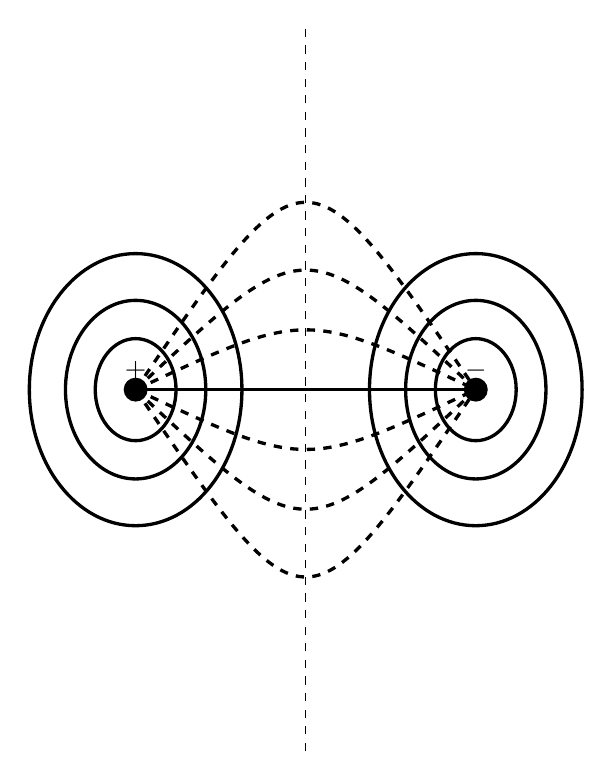
\begin{tikzpicture}[scale=1.35]
  % 电荷：+ 左、- 右
  \fill (-1.6,0) circle (3.2pt);
  \fill (1.6,0) circle (3.2pt);
  \node[above] at (-1.6,0) {$+$};
  \node[above] at (1.6,0) {$-$};
  % 实线：连接两电荷的水平线
  \draw[very thick] (-1.6,0) -- (1.6,0);
  % 实线：电荷周围的闭合等位线（各 3 层）
  \foreach \rx/\ry in {0.38/0.48, 0.66/0.84, 1.0/1.28} {
    \draw[very thick] (-1.6,0) ellipse ({\rx} and {\ry});
    \draw[very thick] (1.6,0) ellipse ({\rx} and {\ry});
  }
  % 虚线：从 + 到 - 的电场线（上下各 3 条弧）
  \foreach \h in {0.75,1.5,2.35} {
    \draw[dashed,very thick] (-1.6,0) .. controls (0,\h) .. (1.6,0);
    \draw[dashed,very thick] (-1.6,0) .. controls (0,-\h) .. (1.6,0);
  }
  % 虚线：竖直中垂线（零等位面），向两端延伸
  \draw[dashed] (0,-3.4) -- (0,3.4);
\end{tikzpicture}
\par\vspace{2pt}
{\small 图 8.}
\end{figure}

% ============================================================
\section{高斯-奥斯特洛格拉德斯基定理及其应用}

我们现在所要讲的定理，是矢量分析中最重要的定理之一。它把 $n$ 阶光滑张量场的面积分与 $(n + 1)$ 阶张量场的体积分联系了起来。

\textbf{定理 1.10}\quad 设给定了光滑张量场 $T_{i_1 i_2 \cdots i_n}(x_1, x_2, x_3)$，则下面的等式成立：

\begin{equation}
\sum_{i_1 = 1}^{3} \int_{V} \frac{\partial}{\partial x_{i_1}} T_{i_1 i_2 \cdots i_n}\, d\tau
= \int_{S} \sum_{i_1 = 1}^{3} T_{i_1 i_2 \cdots i_n}\, dS_{i_1},
\tag{1.34}
\end{equation}

这里 $d\tau$ 是体积元素，$d\ve{S}(dS_1, dS_2, dS_3)$ 为沿着曲面的外法线方向、长度在数值上等于曲面 $S$ 的面积元素的面积的矢量。

\textbf{证明}\quad 考虑任一由封闭曲面 $S$ 所围成的体积 $V$。将这个体积分割为若干个体积元素，使每个体积元素用立方体来逼近时达到给定的精确度。现对棱平行于坐标轴的立方体来证明公式(1.34)。位于等式(1.34)左边的积分，对于立方体可改写成下面的形状：

\begin{equation}
\begin{aligned}
&\int \frac{\partial}{\partial x_1} T_{1 i_2 i_3 \cdots i_n}\, dx_1 dx_2 dx_3
 + \int \frac{\partial}{\partial x_2} T_{2 i_2 i_3 \cdots i_n}\, dx_1 dx_2 dx_3\\
&\qquad + \int \frac{\partial}{\partial x_3} T_{3 i_2 i_3 \cdots i_n}\, dx_1 dx_2 dx_3\\
&= \int T_{1 i_2 i_3 \cdots i_n} \Big|_{x_1}^{x_1 + dx_1} dx_2 dx_3
 + \int T_{2 i_2 i_3 \cdots i_n} \Big|_{x_2}^{x_2 + dx_2} dx_1 dx_3\\
&\qquad + \int T_{3 i_2 i_3 \cdots i_n} \Big|_{x_3}^{x_3 + dx_3} dx_1 dx_2.
\end{aligned}
\tag{1.35}
\end{equation}

由图 9，显然

\begin{figure}[htbp]
\centering
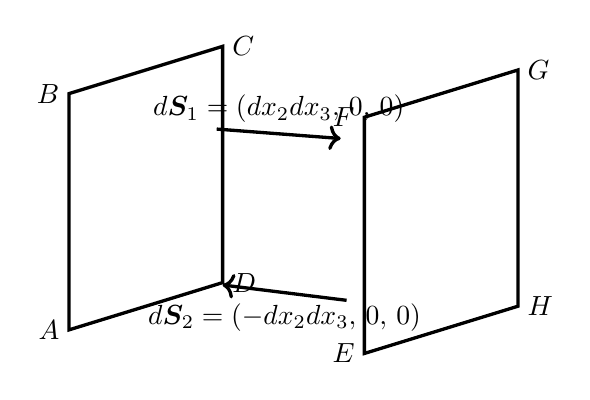
\begin{tikzpicture}[scale=1.5]
  % 左平面 ABCD（平行四边形）
  \coordinate (A) at (0.7,0.8);
  \coordinate (B) at (0.7,2.8);
  \coordinate (C) at (2.0,3.2);
  \coordinate (D) at (2.0,1.2);
  \draw[very thick] (A) -- (B) -- (C) -- (D) -- cycle;
  % 右平面 EFGH
  \coordinate (E) at (3.2,0.6);
  \coordinate (F) at (3.2,2.6);
  \coordinate (G) at (4.5,3.0);
  \coordinate (H) at (4.5,1.0);
  \draw[very thick] (E) -- (F) -- (G) -- (H) -- cycle;
  % 顶点标注
  \node[left]  at (A) {$A$};
  \node[left]  at (B) {$B$};
  \node[right] at (C) {$C$};
  \node[right] at (D) {$D$};
  \node[left]  at (E) {$E$};
  \node[left]  at (F) {$F$};
  \node[right] at (G) {$G$};
  \node[right] at (H) {$H$};
  % 面积元箭头：上（右向）、下（左向），从平面内部出发、到达另一平面
  \draw[->,very thick] (1.95,2.5) -- (3.0,2.42) node[midway,above]{$d\ve{S}_1 = (dx_2 dx_3,\,0,\,0)$};
  \draw[->,very thick] (3.05,1.05) -- (2.0,1.18) node[midway,below]{$d\ve{S}_2 = (-dx_2 dx_3,\,0,\,0)$};
\end{tikzpicture}
\par\vspace{2pt}
{\small 图 9.}
\end{figure}

\begin{equation*}
\begin{aligned}
&\int T_{1 i_2 i_3 \cdots i_n} \Big|_{x_1}^{x_1 + dx_1} dx_2 dx_3\\
&\quad = \int_{ABCD} T_{1 i_2 i_3 \cdots i_n}\, dx_2 dx_3 - \int_{EFGH} T_{1 i_2 i_3 \cdots i_n}\, dx_2 dx_3.
\end{aligned}
\end{equation*}

因除开 $ABCD$ 和 $EFGH$ 外，在其余的所有的边界上有 $dS_1 = 0$，故

\begin{equation}
\int T_{1 i_2 \cdots i_n} \Big|_{x_1}^{x_1 + dx_1} dx_2 dx_3 = \int T_{1 i_2 \cdots i_n}\, dS_1.
\tag{1.36a}
\end{equation}

类似可得
\begin{equation}
\int T_{2 i_2 \cdots i_n} \Big|_{x_2}^{x_2 + dx_2} dx_1 dx_3 = \int T_{2 i_2 \cdots i_n}\, dS_2,
\tag{1.36b}
\end{equation}

\begin{equation}
\int T_{3 i_2 \cdots i_n} \Big|_{x_3}^{x_3 + dx_3} dx_1 dx_2 = \int T_{3 i_2 \cdots i_n}\, dS_3.
\tag{1.36c}
\end{equation}

将等式(1.36a,b,c)代入(1.35)，得(1.34)。于是定理对任一体积元素 $\triangle V$ 都成立。由此即可推出它对整个体积 $V$ 也成立，因为沿着所有立方体表面的积分之和给出了包围整个体积 $V$ 的表面的积分；沿着立方体内侧的积分，由于相邻之面的法线方向相反而相互抵消。定理证毕。

\textbf{例 13}\quad $n = 1$ 的情形。对于 $n = 1$，量 $T_i$ 是矢量的分量。等式(1.34)可改写成

\begin{equation}
\begin{aligned}
\int_{V} \nabla \cdot \ve{F}\, d\tau &= \int_{V} \operatorname{div}\ve{F}\, d\tau = \oint_{S_V} \ve{F} \cdot d\ve{S}\\
&= \oint_{S_V} F_n\, dS,
\end{aligned}
\tag{1.37}
\end{equation}

即通过闭曲面的矢量流量等于该矢量散度的体积分。可以讲，量 $\operatorname{div}\ve{F}$ 代表了所给矢量场源的密度。关于矢量场的高斯-奥斯特洛格拉德斯基（Gauss--Остроградский）定理(1.37)，在叙述中经常会碰到。

$n = 2$ 的情形。有

\begin{equation*}
\sum_{i=1}^{3} \int \frac{\partial}{\partial x_i} T_{ij}\, d\tau = \int \sum_{i=1}^{3} T_{ij}\, dS_i.
\end{equation*}

考虑张量
\begin{equation}
S_{iji_1 \cdots i_n} \equiv \delta_{ij}\, T_{i_1 i_2 \cdots i_n}.
\tag{1.38}
\end{equation}

现证明，在这种情形由高斯-奥斯特洛格拉德斯基定理可推出等式

\begin{equation}
\int \frac{\partial}{\partial x_i} T_{j_1 j_2 \cdots j_n}\, d\tau = \int T_{j_1 j_2 \cdots j_n}\, dS_i
\tag{1.39}
\end{equation}

(1.34)式的直接推论是

\begin{equation}
\sum_{i=1}^{3} S_{iji_1 \cdots i_n}\, dS_i = T_{i_1 i_2 \cdots i_n}\, dS_j.
\tag{1.40}
\end{equation}

将(1.38)式进行微商后再求和，得

\begin{equation}
\sum_{i=1}^{3} \frac{\partial}{\partial x_i} S_{iji_1 \cdots i_n} = \frac{\partial}{\partial x_j} T_{i_1 i_2 \cdots i_n}.
\tag{1.41}
\end{equation}

应用定理 1.10 于(1.41)的左边部分，得

\begin{equation}
\int \sum_{i=1}^{3} \frac{\partial}{\partial x_i} S_{iji_1 i_2 \cdots i_n}\, d\tau = \sum_{i=1}^{3} \int S_{iji_1 i_2 \cdots i_n}\, dS_i,
\tag{1.42}
\end{equation}

由(1.41)和(1.42)推出

\begin{equation*}
\int T_{i_1 i_2 \cdots i_n}\, dS_j = \int \frac{\partial}{\partial x_j} T_{i_1 i_2 \cdots i_n}\, d\tau.
\end{equation*}

现在，(1.39)式就成为显然的事了。

现举例说明高斯-奥斯特洛格拉德斯基定理对某些物理问题的应用。

\textbf{1. 不可压缩流体的连续性方程}\quad 取密度为 $\rho$，运动速度为 $\ve{v}$，体积为 $V$ 的流体。量 $\frac{\partial}{\partial t} \int \rho\, d\tau$ 等于在体积 $V$ 内流体质量的改变速率，而量 $\int \rho\ve{v} \cdot d\ve{S}$ 为单位时间内流经物体 $V$ 的边界 $S$ 的流体质量。由质量守恒定律推出

\begin{equation*}
\frac{\partial}{\partial t} \int_{V} \rho\, d\tau + \int_{S_V} \rho\ve{v} \cdot d\ve{S} = 0,
\end{equation*}

或
\begin{equation}
\int_{V} \left[\frac{\partial\rho}{\partial t} + \nabla \cdot (\rho\ve{v})\right] d\tau = 0.
\tag{1.43}
\end{equation}

因(1.43)对任意体积 $V$ 都成立，故

\begin{equation*}
\frac{\partial\rho}{\partial t} + \nabla \cdot (\rho\ve{v}) = 0.
\end{equation*}

此即为不可压缩流体的连续性方程。

\textbf{2. 力线管}\quad 如果在空间 $R$ 的某个区域内 $\nabla \cdot \ve{A} = 0$，则该区域内矢量 $\ve{A}$ 的力线是不中断的。画出矢量 $\ve{A}$ 的力线，并考虑与垂直于矢量 $\ve{A}$ 的面 $S_1$ 和 $S_2$ 相交的力线的管。由高斯-奥斯特洛格拉德斯基定理推出下面的恒等式：

\begin{equation*}
\begin{aligned}
\int_{S_V} \ve{A} \cdot d\ve{S} &= \int_{S_1} \ve{A} \cdot d\ve{S} + \int_{S_2} \ve{A} \cdot d\ve{S}\\
&= \int_{V} \nabla \cdot \ve{A}\, d\tau = 0,
\end{aligned}
\end{equation*}

这里 $S_V$ 是由力线管所围体积 $V$ 的全表面。因为矢量 $\ve{A}$ 与 $d\ve{S}$ 正交，所以在管的侧面上的积分等于零。由定义，$\int_{S_1} \ve{A} \cdot d\ve{S}$ 是与 $S_1$ 相交的力线数目，而 $\int_{S_2} \ve{A} \cdot d\ve{S}$ 是与 $S_2$ 相交的力线数目。因 $S_1$ 和 $S_2$ 可以取得任意小，力线必须是连续的，即必须或者是闭合，或者从 $-\infty$ 远处延伸到 $+\infty$ 远处。因此，力线仅在 $\nabla \cdot \ve{A} \neq 0$ 的那些点上出发或终止。今考虑特殊情形。

1）如果 $\ve{H}$ 是磁场矢量，则 $\nabla \cdot \ve{H} = 0$。众所周知，磁荷实际上是不存在的。

2）在静电场中，有方程 $\nabla \cdot \ve{E} = 4\pi\rho$，这里 $\ve{E}$ 是电场矢量，$\rho$ 为电荷密度。电场的力线即电力线在电荷处或无穷远处出发或终止。

\textbf{3. 应力张量}\quad 考虑一浸没在介质（固体的、液体的或气体的）之中的物体。一般说来，作用于它的不只有形如 $\int \ve{F}\, d\tau$ 的力（重力或者作用于带电物体上的电场力），而且还有表面力，因为物体的每一个表面元素和其周围介质是相互作用的。

设 $f_i$ 是作用在曲面元素 $d\ve{S}$ 上的力，且作用点在体积表面的外侧。我们可假定（至少对充分小的面积）$f_i$ 与曲面元素的面积成正比：

\begin{equation*}
f_i = \sum_{j} T_{ij}\, dS_j.
\end{equation*}

因 $\ve{f}$ 与 $d\ve{S}$ 是矢量，故量 $T_{ij}$ 应该是二阶张量。此张量就称为应力张量。这样一来，由高斯-奥斯特洛格拉德斯基定理知，作用在物体上的合力就等于

\begin{equation}
\int_{V} F_i\, d\tau + \sum_{j} \int_{S} T_{ij}\, dS_j = \int_{V} \left(F_i + \sum_{j} \frac{\partial T_{ij}}{\partial x_j}\right) d\tau.
\tag{1.44a}
\end{equation}

由此看出，表面力可用等价的体积力来代替〔在满足等式(1.44a)的意义上〕。

由牛顿第二定律，

\begin{equation}
(F)_i = \int \rho\, a_i\, d\tau,
\tag{1.45}
\end{equation}

这里 $\ve{a}$ 为加速度，$\rho$ 为物体的密度。因(1.45)对任意的体积 $V$ 都成立，故得运动方程

\begin{equation}
\rho\, a_i = F_i + \sum_{j} \frac{\partial T_{ij}}{\partial x_j}
\tag{1.46}
\end{equation}

应力张量的物理意义是怎样的呢？命矢量 $d\ve{S}$ 平行于坐标轴 $x_1$，则由等式

\begin{equation*}
f_i = T_{i1}\, dS_1 + T_{i2}\, dS_2 + T_{i3}\, dS_3
\end{equation*}

推出
\begin{equation*}
f_1 = T_{11}\, dS, \qquad f_2 = T_{21}\, dS, \qquad f_3 = T_{31}\, dS.
\end{equation*}

当矢量 $d\ve{S}$ 平行于坐标轴 $x_2$ 或 $x_3$ 时，也可得类似的结果：

\begin{equation*}
\begin{aligned}
f_1 &= T_{12}\, dS, \quad f_2 = T_{22}\, dS, \quad f_3 = T_{32}\, dS,\\
f_1 &= T_{13}\, dS, \quad f_2 = T_{23}\, dS, \quad f_3 = T_{33}\, dS.
\end{aligned}
\end{equation*}

今选取坐标系的轴，使

\begin{equation*}
T_{ij} = \lambda_i\, \delta_{ij}.
\end{equation*}

则对矢量 $d\ve{S}$ 平行于 $x_1$ 轴的物体，有

\begin{equation*}
f_1 = \lambda_1\, dS, \qquad f_2 = f_3 = 0.
\end{equation*}

在这种情形，作用在物体上的力，是沿着 $x_1$ 轴的拉力 $(\lambda_1 > 0)$ 或压力 $(\lambda_1 < 0)$。

此外，当矢量 $d\ve{S}$ 为任意方向的情形，则物体处于剪应力的作用下。

\textbf{例 14}\quad 理想（无粘性）流体。作用在理想流体的任一表面元素上的力，与该曲面相垂直。因此，对于理想流体，在任一坐标系中的应力张量均为

\begin{equation*}
T_{ij} = -P\, \delta_{ij},
\end{equation*}

这里 $P$ 为某个坐标的函数。因此由(1.46)式，任一质点的运动方程为

\begin{equation*}
\rho\, \ve{a} = \ve{F} - \nabla P.
\end{equation*}

今计算加速度 $\ve{a}$。设 $\ve{v} = \ve{v}(\ve{r}, t)$；又设当 $t = t_0$ 时，$\ve{r} = \ve{r}_0$；当 $t = t_0 + \delta t$ 时，$\ve{r} = \ve{r}_0 + \ve{v}\,\delta t$，利用泰勒公式得

\begin{equation*}
\begin{aligned}
\ve{a}\,\delta t &= \ve{v}(\ve{r}_0 + \ve{v}\,\delta t,\ t_0 + \delta t) - \ve{v}(\ve{r}_0, t_0)\\
&= \frac{\partial\ve{v}}{\partial t}\,\delta t + \sum_{i=1}^{3} \delta r_i\, \frac{\partial\ve{v}}{\partial x_i}\\
&= \left[\frac{\partial\ve{v}}{\partial t} + (\ve{v} \cdot \nabla)\ve{v}\right] \delta t.
\end{aligned}
\end{equation*}

即
\begin{equation*}
\rho \left[(\ve{v} \cdot \nabla)\ve{v} + \frac{\partial\ve{v}}{\partial t}\right] = \ve{F} - \nabla P.
\end{equation*}

\textbf{4. 静电场}\quad 考虑安置在原点的点电荷 $e$，电荷密度 $\sigma(\ve{r})$ 用下式定义：

\begin{equation*}
\sigma(\ve{r}) =
\begin{cases}
\infty, & \text{当 } r = 0 \text{ 时},\\
0,     & \text{当 } r \neq 0 \text{ 时},
\end{cases}
\end{equation*}

但
\begin{equation*}
\int \sigma(\ve{r})\, d\tau = e
\end{equation*}

（这里的积分区域取在包含原点的全空间上）。

置
\begin{equation*}
\delta^{3}(\ve{r}) \equiv \frac{\sigma(\ve{r})}{e},
\end{equation*}

或
\begin{equation*}
\delta^{3}(\ve{r}) \equiv \delta(x)\, \delta(y)\, \delta(z),
\end{equation*}

同时
\begin{equation*}
\delta(x_i) = 0, \quad \text{当 } x_i \neq 0;
\end{equation*}

而
\begin{equation*}
\int_{-a}^{b} \delta(x_i)\, dx_i = 1 \qquad (a, b > 0).
\end{equation*}

量 $\delta(x)$ 称为狄拉克（Dirac）$\delta$-函数。此函数不符合古典函数的定义，但它可以表示成某个函数序列的极限，且这个序列中的每个函数的图象的宽度逐渐减小，并向上面拉长，以使得每条曲线与 $x$ 轴所围成的面积等于 1。例如

\begin{equation*}
\delta(x) = \lim_{a \to 0} f_a(x),
\end{equation*}

这里
\begin{equation*}
f_a(x) = \frac{1}{a\sqrt{\pi}}\, e^{-x^{2}/a^{2}}.
\end{equation*}

引进了诸如狄拉克 $\delta$-函数的符号以后，就给物理学家以将基本粒子看作一个点来研究的可能性。

现回到我们所研究的例子。点电荷场的位势为

\begin{equation*}
\Phi = \frac{e}{|\ve{r}|}.
\end{equation*}

此时电场强度等于

\begin{equation*}
\ve{E} = -\nabla\Phi = \frac{e}{|\ve{r}|^{3}}\, \ve{r},
\end{equation*}

矢量 $\ve{E}$ 的散度等于

\begin{equation*}
\begin{aligned}
\nabla \cdot \ve{E} &= \sum_{i} \frac{\partial}{\partial x_i} \left(\frac{e}{|\ve{r}|^{3}}\, x_i\right)\\
&= \frac{3e}{|\ve{r}|^{3}} - \frac{3e}{|\ve{r}|^{4}} \sum_{i} \frac{x_i^{2}}{|\ve{r}|} = 0. \qquad (\text{当 } r \neq 0)
\end{aligned}
\end{equation*}

但在坐标原点微商运算没有定义。此时利用高斯-奥斯特洛格拉德斯基定理：

\begin{equation*}
\int \nabla \cdot \ve{E}\, d\tau = \int \ve{E} \cdot d\ve{S} = \int \frac{e}{|\ve{r}|^{2}}\, |\ve{r}|^{2}\, d\Omega = 4\pi e.
\end{equation*}

左边的积分区域取在包围原点的球上。因此，如果 $\sigma(\ve{r}) = e\,\delta^{3}(\ve{r})$，则

\begin{equation}
\nabla \cdot \ve{E} = 4\pi e\, \delta^{3}(\ve{r}), \qquad \text{或} \quad -\nabla^{2}\Phi = 4\pi e\, \delta^{3}(\ve{r}).
\tag{1.47}
\end{equation}

注意，对 $\delta$-函数的运算有怀疑的读者，可利用高斯分布及极限过程，也能得到同样的结果。

现假定电荷分布的密度是任意的。给定分布密度的电位可用下式表示：

\begin{equation}
\Phi(\ve{r}) = \int \frac{\sigma(\ve{r}')}{|\ve{r} - \ve{r}'|}\, d\tau'.
\tag{1.48}
\end{equation}

将算子 $\nabla^{2}$ 作用于(1.48)式，得

\begin{equation}
\nabla^{2}\Phi(\ve{r}) = -\int \sigma(\ve{r}')\, 4\pi\, \delta^{3}(\ve{r} - \ve{r}')\, d\tau'.
\tag{1.49}
\end{equation}

因由等式
\begin{equation*}
\nabla^{2}\, \frac{1}{|\ve{r}|} = -4\pi\, \delta^{3}(\ve{r})
\end{equation*}

推出
\begin{equation}
\nabla^{2}\left(\frac{1}{|\ve{r} - \ve{r}'|}\right) = -4\pi\, \delta^{3}(\ve{r} - \ve{r}'),
\tag{1.49a}
\end{equation}

所以(1.49)显然成立。由 $\delta$ 函数的性质直接推出

\begin{equation}
\int f(\ve{r})\, \delta^{3}(\ve{r})\, d\tau = f(0)
\tag{1.50}
\end{equation}

将(1.50)代入(1.49)的右边，就得电荷分布密度为任意时的电位 $\Phi$ 的方程：

\begin{equation}
\nabla^{2}\Phi = -4\pi\, \sigma(\ve{r}).
\tag{1.51}
\end{equation}

方程(1.51)称为泊松（Poisson）方程〔而方程 $\nabla^{2}\Phi = 0$ 称为拉普拉斯（Laplace）方程〕。

\textbf{附注：}关系式 $\nabla \cdot \ve{E} = 4\pi\rho$ 是麦克斯韦（Maxwell）方程组中的一个方程。

方程(1.51)的通解为

\begin{equation*}
\Phi = \Phi_0 + \int \frac{\sigma(\ve{r}')}{|\ve{r} - \ve{r}'|}\, d\tau',
\end{equation*}

这里 $\Phi_0$ 满足拉普拉斯方程 $\triangle\Phi = 0$。事实上，设

\begin{equation*}
\Phi_0 \equiv \Phi - \int \frac{\sigma(\ve{r}')}{|\ve{r} - \ve{r}'|}\, d\tau',
\end{equation*}

则得
\begin{equation*}
\begin{aligned}
\nabla^{2}\Phi_0 &= \nabla^{2}\Phi - \nabla^{2} \int \frac{\sigma(\ve{r}')}{|\ve{r} - \ve{r}'|}\, d\tau' = -4\pi\sigma + 4\pi\sigma = 0.
\end{aligned}
\end{equation*}

这里对方程(1.51)所得的结果，事实上可引出更为一般的结果，并可应用到相当广泛的一类线性方程中去。

设 $H$ 为线性算子，即具有下面性质的算子：

\begin{equation*}
H(a\varphi + b\psi) = a\, H\varphi + b\, H\psi.
\end{equation*}

如果
\begin{equation}
H\Phi = f(\ve{r}),
\tag{1.51a}
\end{equation}

而函数 $G(\ve{r})$ 使

\begin{equation*}
H\, G(\ve{r}) = \delta^{3}(\ve{r})
\end{equation*}

[这样的函数 $G(\ve{r})$ 叫做方程(1.51a)的格林（Green）函数]，则方程(1.51a)的解可以表示成

\begin{equation*}
\Phi(\ve{r}) = \int G(\ve{r} - \ve{r}')\, f(\ve{r}')\, d\tau' + \Phi_0(\ve{r}),
\end{equation*}

这里 $H\Phi_0 = 0$。事实上，设

\begin{equation*}
\Phi_0 \equiv \Phi - \int G(\ve{r} - \ve{r}')\, f(\ve{r}')\, d\tau',
\end{equation*}

则有
\begin{equation*}
\begin{aligned}
H\Phi_0 &= H\Phi - \int H\, G(\ve{r} - \ve{r}')\, f(\ve{r}')\, d\tau'\\
&= H\Phi - \int \delta^{3}(\ve{r} - \ve{r}')\, f(\ve{r}')\, d\tau'\\
&= H\Phi(\ve{r}) - f(\ve{r}) = 0.
\end{aligned}
\end{equation*}

当非齐次方程所对应的齐次方程的通解为已知时，常广泛地应用此法去求它的解。这种方法通常叫做“格林函数法”。在第五章中我们将会介绍。

\textbf{5. 热传导}\quad 引进下面的记号：

\begin{itemize}[leftmargin=2.5em,itemsep=1pt]
\item $k$——热传导系数；
\item $T$——温度；
\item $Q$——在单位时间内通过单位面积的热量（热流量）。
\end{itemize}

由热力学中熟知的关系式

\begin{equation*}
\ve{Q} = -k\, \nabla T
\end{equation*}

可知，如果 $\varepsilon$ 为在容积 $V$ 中的能量，则由能量守恒定律推出

\begin{equation*}
\frac{\partial}{\partial t} \int_{V} \varepsilon\, d\tau + \int_{S_V} \ve{Q} \cdot d\ve{S} = 0.
\end{equation*}

但 $\varepsilon = cT$（$c$ 为比热），因此

\begin{equation*}
\int_{V} \left[c\, \frac{\partial T}{\partial t} + \nabla \cdot \ve{Q}\right] d\tau = 0.
\end{equation*}

因这个方程对任何容积 $V$ 都成立，所以

\begin{equation*}
c\, \frac{\partial T}{\partial t} = -\nabla \cdot \ve{Q} = k\, \nabla^{2} T.
\end{equation*}

最后一个关系式常称为热传导方程。

% ============================================================
\section{斯托克斯定理及其应用}

高斯-奥斯特洛格拉德斯基定理建立了体积分和曲面积分之间的联系。斯托克斯（Stokes）定理则建立了曲面积分和封闭围道曲线积分之间的联系，而这里的曲面即张在该闭曲线之上。

假定 $S$ 是某个非闭曲面，它张在闭围道 $L$ 之上，$d\ve{S}$ 为曲面元素，$d\ve{l}$ 为弧元素。则下面的定理成立：

\textbf{定理 1.11}（斯托克斯定理）\quad 矢量场 $\ve{A}$ 沿着闭围道 $L$ 的环量等于矢量 $\nabla \times \ve{A}$ 通过张在此围道上的任一曲面的流量：

\begin{equation}
\oint_{L} \ve{A} \cdot d\ve{l} = \int_{S} \nabla \times \ve{A} \cdot d\ve{S}.
\tag{1.52}
\end{equation}

\textbf{证明}\quad 考虑长方形面积元素（图 10）。如果我们考虑的是标量，则坐标轴的定向可任意选取。现在选取坐标轴，使它和长方形的两条边重合。这时有

\begin{figure}[htbp]
\centering
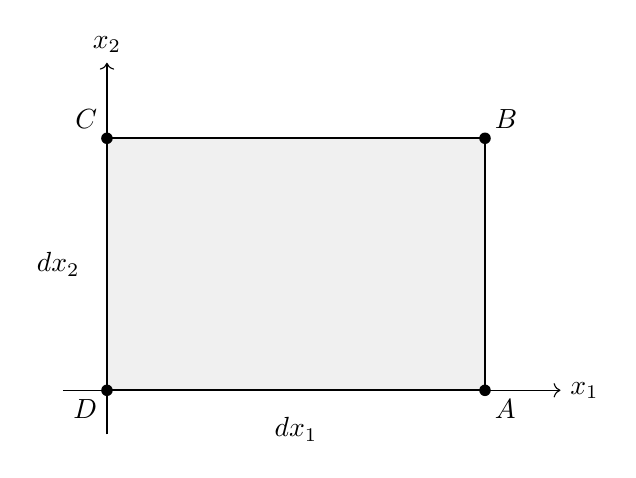
\begin{tikzpicture}[scale=1.6]
  % 坐标轴（矩形位于 x1-x2 平面，法向沿 x3）
  \draw[->] (-0.35,0) -- (3.6,0) node[right]{$x_1$};
  \draw[->] (0,-0.35) -- (0,2.6) node[above]{$x_2$};
  % 矩形：D 在原点，A 在 x1 轴上，C 在纵轴上，B 为右上角
  \coordinate (D) at (0,0);
  \coordinate (A) at (3.0,0);
  \coordinate (B) at (3.0,2.0);
  \coordinate (C) at (0,2.0);
  \fill[gray!12] (D) -- (A) -- (B) -- (C) -- cycle;
  \draw[thick] (D) -- (A) -- (B) -- (C) -- cycle;
  \fill (D) circle (1.3pt) node[below left]{$D$};
  \fill (A) circle (1.3pt) node[below right]{$A$};
  \fill (B) circle (1.3pt) node[above right]{$B$};
  \fill (C) circle (1.3pt) node[above left]{$C$};
  % 边长标注
  \node[below] at (1.5,-0.14) {$dx_1$};
  \node[left] at (-0.14,1.0) {$dx_2$};
\end{tikzpicture}
\par\vspace{2pt}
{\small 图 10.}
\end{figure}

\begin{equation*}
d\ve{S} = dx_1\, dx_2\, \ve{k}.
\end{equation*}

计算(1.52)式右边部分的积分：

\begin{equation*}
\begin{aligned}
\int \nabla \times \ve{A} \cdot d\ve{S}
&= \iint \left(\frac{\partial A_2}{\partial x_1} - \frac{\partial A_1}{\partial x_2}\right) dx_1 dx_2\\
&= \left.\int A_2\, dx_2\right|_{x_1}^{x_1 + dx_1} - \left.\int A_1\, dx_1\right|_{x_2}^{x_2 + dx_2}
\end{aligned}
\end{equation*}

但
\begin{equation*}
\begin{aligned}
\left.\int A_2\right|_{x_1}^{x_1 + dx_1} dx_2 &= \int_{A}^{B} A_2\, dx_2 - \int_{D}^{C} A_2\, dx_2\\
&= \int_{A}^{B} A_2\, dx_2 + \int_{C}^{D} A_2\, dx_2 = \oint A_2\, dx_2.
\end{aligned}
\end{equation*}

另一积分也作相类似的运算后，(1.52)的右边部分即可化成：

\begin{equation}
\iint \left(\frac{\partial A_2}{\partial x_1} - \frac{\partial A_1}{\partial x_2}\right) dx_1 dx_2 = \oint \ve{A} \cdot d\ve{l}.
\tag{1.53}
\end{equation}

这样一来，对于长方形面积元素，定理得证。对于分块光滑的曲面，我们可将它划分为许多个长方形面积元素。应用斯托克斯定理于每一个这种长方形面积元素，并将所得的等式相加，则容易证明斯托克斯定理对于一般情形也是成立的。事实上，两个相邻长方形在邻接边处的各自的走向，正好相反。因此在(1.53)型等式相加时，左边只剩下沿着最外边界（围道 $L$）的曲线积分。

\textbf{附注：}也可对 $n$ 阶张量场作出斯托克斯定理。

今考虑斯托克斯定理在场论中的一些应用。

\textbf{无旋矢量场和位势矢量场。}如果矢量场 $\ve{A}$ 在某个区域 $R$ 内

\begin{equation*}
\nabla \times \ve{A} = 0,
\end{equation*}

则称此场在 $R$ 内是无旋的；如果存在连续标量场 $\Phi$，使在域 $R$ 内处处有

\begin{equation*}
\ve{A} = \nabla\Phi,
\end{equation*}

则称场 $\ve{A}$ 为位势场，而函数 $\Phi$ 称为矢量场 $\ve{A}$ 的位势。

显然，所有位势场都是无旋的，反之则仅对单连通区域才成立。现引进单连通区域的概念。

空间区域 $R$ 称为单连通的，如果位于它里面的任意一条闭曲线 $C$，可以作收缩于一点的连续变形而不超出此区域的范围。

这样，图 11 上的区域 (I) 是平面上的单连通区域，而 (II) 是非单连通区域。在空间中，球、所有凸容积，不仅是整个地，也可以是带有空腔的（例如球带）都可作为单连通区域的例子。而非单连通区域的例子则可举出环面、有空腔的无限圆柱体空间等。

\begin{figure}[htbp]
\centering
\begin{tikzpicture}[scale=1.05]
  % (I) 单连通区域：斜线阴影的圆盘
  \begin{scope}
    \fill[pattern=north east lines, pattern color=gray!50] (0,0) circle (1.3);
    \draw[thick] (0,0) circle (1.3);
    \node at (-1.62,1.32) {Ⅰ};
  \end{scope}
  % (II) 非单连通区域：斜线阴影的圆环
  \begin{scope}[xshift=4.3cm]
    \fill[pattern=north east lines, pattern color=gray!50] (0,0) circle (1.4);
    \fill[white] (0,0) circle (0.6);
    \draw[thick] (0,0) circle (1.4);
    \draw[thick] (0,0) circle (0.6);
    \node at (-1.78,1.42) {Ⅱ};
  \end{scope}
\end{tikzpicture}
\par\vspace{2pt}
{\small 图 11.}
\end{figure}

\begin{figure}[htbp]
\centering
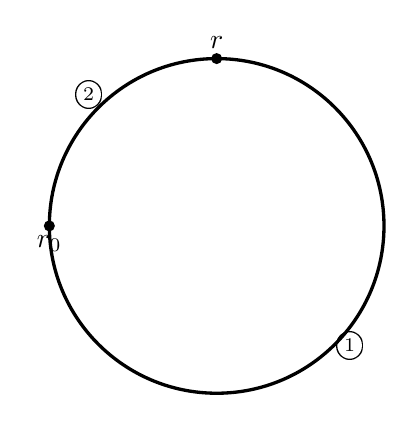
\begin{tikzpicture}[scale=1.25]
  % 闭围道 C（圆），r₀ 在左侧，两条路径 ①、②
  \draw[very thick] (0,0) circle (1.7);
  % 左边缘的点 r₀
  \fill (-1.7,0) circle (1.6pt);
  \node[below] at (-1.7,0) {$r_0$};
  % 顶部点 r
  \fill (0,1.7) circle (1.6pt);
  \node[above] at (0,1.7) {$r$};
  % 路径 ①（右下弧）与 ②（左上弧）
  \node at (1.35,-1.25) {\textcircled{\scriptsize 1}};
  \node at (-1.3,1.3) {\textcircled{\scriptsize 2}};
\end{tikzpicture}
\par\vspace{2pt}
{\small 图 12.}
\end{figure}

在单连通区域内，于每个闭曲线 $C$ 上都可张上整个都在此区域内的分块光滑曲面。

\textbf{定理 1.12}\quad 如果 $R$ 是单连通区域，且在 $R$ 内处处有 $\nabla \times \ve{A} = 0$，则矢量场 $\ve{A}$ 为位势场。即存在 $\Phi$，使 $\nabla\Phi = \ve{A}$。

\textbf{证明}\quad 在 $R$ 内取点 $\ve{r}_0$，置

\begin{equation*}
\Phi(\ve{r}) \equiv \int_{\ve{r}_0}^{\ve{r}} \ve{A} \cdot d\ve{l}
\end{equation*}

（沿着任意路径）。于是由斯托克斯定理及等式 $\nabla \times \ve{A} = 0$ 推出

\begin{equation*}
\oint \ve{A} \cdot d\ve{l} = \int_{S} \nabla \times \ve{A} \cdot d\ve{S} = 0.
\end{equation*}

现在显然
\begin{equation*}
\oint \ve{A} \cdot d\ve{l} = 0 = \int_{\text{\textcircled{\scriptsize 1}}\ \ve{r}_0}^{\ve{r}} \ve{A} \cdot d\ve{l} - \int_{\text{\textcircled{\scriptsize 2}}\ \ve{r}_0}^{\ve{r}} \ve{A} \cdot d\ve{l}.
\end{equation*}

所以 $\Phi(\ve{r})$ 仅是 $\ve{r}$ 的函数。再因

\begin{equation*}
\frac{d}{dx} \int_{0}^{x} f(y)\, dy = f(x),
\end{equation*}

故容易断定
\begin{equation*}
\ve{A} = \nabla\Phi.
\end{equation*}

显然，用矢量场 $\ve{A}$ 确定的标量场 $\Phi$，可精确到一常数被加项，因为

\begin{equation*}
\ve{A} = \nabla\Phi_1 = \nabla\Phi_2, \qquad \Phi_1 - \Phi_2 = \text{const}.
\end{equation*}

\textbf{附注：}区域 $R$ 必须是单连通的。否则 $\oint \ve{A} \cdot d\ve{l}$ 不等于 0。例如，沿着图 13 上的路径且在孔内 $\nabla \times \ve{A} \neq 0$ 的话。不过多连通域可以单连通化。如图 14 所画的那样将它剪开，则带斜线的区域就是单连通的了。但一般说来，这里已经是 $\Phi_{+} \neq \Phi_{-}$，其中

\begin{equation*}
\Phi_{+}(\ve{r}) = \int_{\ve{r}}^{\ve{a}} \ve{A} \cdot d\ve{l}, \qquad \Phi_{-}(\ve{r}) = \int_{\ve{r}}^{\ve{b}} \ve{A} \cdot d\ve{l}.
\end{equation*}

（参看图 14）。因此，无旋矢量场 $\ve{A}$ 在整个区域 $R$ 内不是位势场，因在位势场内函数 $\Phi$ 必须是单值的。如果一场在 $R$ 内的每一点的邻域内都可构造一函数 $\Phi$（局部位势），则称此场为局部位势场。但函数 $\Phi$ 在全域内不再是单值的（多值位势）。

\begin{figure}[htbp]
\centering
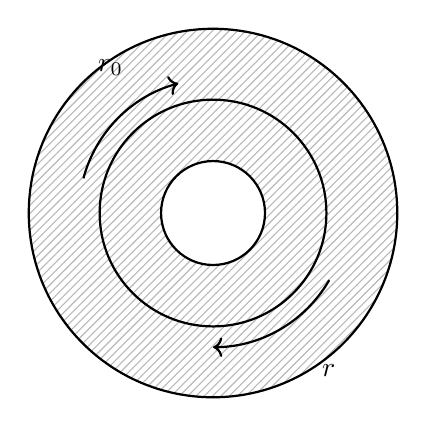
\begin{tikzpicture}[scale=1.2]
  % 圆环区域 r₀ < r < R：斜线阴影，三个同心圆
  \fill[pattern=north east lines, pattern color=gray!55] (0,0) circle (1.95);
  \fill[white] (0,0) circle (0.55);
  \draw[thick] (0,0) circle (1.95);
  \draw[thick] (0,0) circle (0.55);
  \draw[thick] (0,0) circle (1.2);
  % 顺时针旋转箭头（左上、右下），标注 r₀ 与 r
  \draw[->,thick] (0,0) ++(165:1.42) arc[start angle=165, delta angle=-60, radius=1.42];
  \node[above left] at (-0.85,1.35) {$r_0$};
  \draw[->,thick] (0,0) ++(330:1.42) arc[start angle=330, delta angle=-60, radius=1.42];
  \node[below right] at (1.05,-1.5) {$r$};
\end{tikzpicture}
\par\vspace{2pt}
{\small 图 13.}
\end{figure}

\begin{figure}[htbp]
\centering
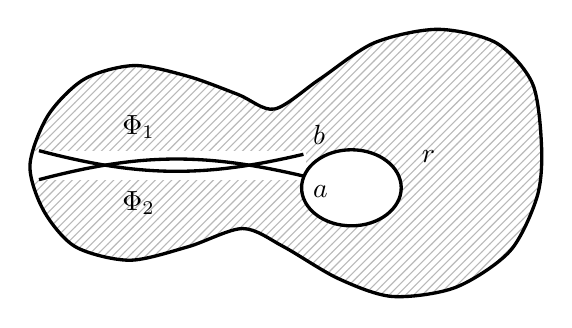
\begin{tikzpicture}[scale=1.15]
  % 外边界：哑铃形（左侧凸起较小，右侧凸起较大，光滑曲线）
  \def\peanut{(-2.7,0) (-2.5,0.55) (-2.1,0.95) (-1.55,1.1) (-0.95,0.98)
              (-0.4,0.78) (0.0,0.62) (0.5,0.95) (1.1,1.35) (1.8,1.5)
              (2.45,1.35) (2.85,0.9) (2.95,0.2) (2.9,-0.35) (2.6,-0.95)
              (2.0,-1.35) (1.3,-1.45) (0.7,-1.25) (0.1,-0.9) (-0.35,-0.7)
              (-0.95,-0.9) (-1.6,-1.05) (-2.2,-0.9) (-2.55,-0.5)}
  \fill[pattern=north east lines, pattern color=gray!55] plot[smooth cycle] coordinates {\peanut};
  % 孔（内边界，近似椭圆，偏右下方）
  \fill[white] (0.85,-0.25) ellipse (0.55 and 0.42);
  % 割线通道（从左侧边界到孔，略带弧度）
  \fill[white] (-2.7,-0.16) rectangle (0.35,0.16);
  % 边界线
  \draw[very thick] plot[smooth cycle] coordinates {\peanut};
  \draw[very thick] (0.85,-0.25) ellipse (0.55 and 0.42);
  % 割线上下缘（略带弧度、向右端略收拢）
  \draw[very thick] (-2.6,0.16) to[bend right=14] (0.32,0.12);
  \draw[very thick] (-2.6,-0.16) to[bend left=14] (0.32,-0.12);
  % 标注：Φ₁ Φ₂、a、b、r
  \node at (-1.5,0.42) {$\Phi_1$};
  \node at (-1.5,-0.42) {$\Phi_2$};
  \node[above right] at (0.32,0.12) {$b$};
  \node[below right] at (0.32,-0.12) {$a$};
  \node at (1.7,0.1) {$r$};
\end{tikzpicture}
\par\vspace{2pt}
{\small 图 14.}
\end{figure}

\textbf{例 15}\quad 静磁学。静磁学方程为

\begin{equation*}
\nabla \times \ve{H} = \frac{4\pi}{c}\, \ve{j},
\end{equation*}

这里 $\ve{H}$ 为磁场矢量，$\ve{j}$ 为流密度。如果在容积 $V$ 内 $\ve{j} \neq 0$，在 $V$ 外 $\ve{j} = 0$，则场 $\ve{H}$ 在 $V$ 外将是无旋的。那么场 $\ve{H}$ 是否是位势场？

如果容积 $V$ 有界，则在 $V$ 外

\begin{equation*}
\ve{H} = \nabla\Phi;
\end{equation*}

如果容积 $V$ 是无界的（流量管），则矢量场 $\ve{H}$ 是非位势的（局部位势）。

% ============================================================
\section{亥姆霍兹定理．麦克斯韦方程}

现在我们叙述并证明一个重要定理。此定理给出了将任一矢量场表示成某个标量函数 $\Phi$ 的梯度与某个散度为零的矢量函数 $\ve{A}$ 的旋度之和。

\textbf{定理 1.13}〔亥姆霍兹（Helmholtz）定理〕\quad 在全空间 $R$ 内单值、连续、有界的矢量场 $\ve{F}$，可分解成位势矢量场和无旋矢量场之和。即可表示为

\begin{equation}
\ve{F} = -\nabla\Phi + \nabla \times \ve{A}, \qquad \text{同时} \quad \nabla \cdot \ve{A} = 0
\tag{1.54}
\end{equation}

标量函数 $\Phi$ 称为矢量场 $\ve{F}$ 的标量位势，而矢量函数 $\ve{A}$ 称为场 $\ve{F}$ 的矢量位势。

\textbf{证明}\quad 定理的证明归结为对所给场 $\ve{F}$，构造满足等式(1.54)的位势 $\Phi$ 和 $\ve{A}$。证明分三步进行。先对两个特殊情形证明定理，尔后推广所得定理于一般情形。

\textbf{1.}\quad 假定所给的矢量场 $\ve{F}$ 满足条件

\begin{equation}
|\ve{F}| < \frac{k}{r^{2+\eta}}, \qquad \eta > 0 \quad (\text{当 } r \to \infty \text{ 时}).
\tag{1.55}
\end{equation}

考虑函数
\begin{equation*}
\ve{G}(\ve{r}) \equiv \int_{\tau} \frac{\ve{F}(\ve{r}')\, d\tau'}{|\ve{r} - \ve{r}'|}.
\end{equation*}

由于所加的条件，此积分收敛，且函数 $\ve{G}(\ve{r})$ 可单值地确定。其次容易验证等式

\begin{equation*}
\nabla^{2}\ve{G}(\ve{r}) = -4\pi\, \ve{F}(\ve{r}).
\end{equation*}

应用(1.33)式于矢量函数 $\ve{G}(\ve{r})$，

\begin{equation*}
\nabla^{2}\ve{G}(\ve{r}) = \nabla[\nabla \cdot \ve{G}(\ve{r})] - \nabla \times [\nabla \times \ve{G}(\ve{r})].
\end{equation*}

现在利用所得的公式，可将函数 $\ve{F}$ 写成

\begin{equation*}
\begin{aligned}
\ve{F} &= -\frac{1}{4\pi} [\nabla(\nabla \cdot \ve{G}) - \nabla \times (\nabla \times \ve{G})]\\
&= -\nabla\Phi + \nabla \times \ve{A},
\end{aligned}
\end{equation*}

式中
\begin{equation*}
\Phi(\ve{r}) = \frac{1}{4\pi}\, \nabla \cdot \ve{G},
\end{equation*}

\begin{equation*}
\ve{A}(\ve{r}) = \frac{1}{4\pi}\, \nabla \times \ve{G}.
\end{equation*}

换言之，在条件(1.55)下，定理得证。若利用函数 $|\ve{r} - \ve{r}'|$ 的对称性，则可将位势 $\Phi$ 和 $\ve{A}$ 表示成更简单的形式。为此，变换 $\nabla_{\ve{r}} \cdot \ve{G}(\ve{r})$ 和 $\nabla_{\ve{r}} \times \ve{G}(\ve{r})$：

\begin{equation*}
\begin{aligned}
\nabla_{\ve{r}} \cdot \ve{G}(\ve{r}) &= \int \nabla_{\ve{r}} \cdot \left(\frac{\ve{F}(\ve{r}')}{|\ve{r} - \ve{r}'|}\right) d\tau'\\
&= \int \ve{F}(\ve{r}') \cdot \nabla_{\ve{r}} \left(\frac{1}{|\ve{r} - \ve{r}'|}\right) d\tau'.
\end{aligned}
\end{equation*}

因
\begin{equation*}
\frac{\partial}{\partial x_i} f(\ve{r} - \ve{r}') = -\frac{\partial}{\partial x_i'}\, f(\ve{r} - \ve{r}'),
\end{equation*}

故有
\begin{equation*}
\nabla_{\ve{r}} \cdot \ve{G}(\ve{r}) = -\int \nabla_{\ve{r}'} \cdot \left(\frac{\ve{F}(\ve{r}')}{|\ve{r} - \ve{r}'|}\right) d\tau' + \int \frac{\nabla_{\ve{r}'} \cdot \ve{F}(\ve{r}')}{|\ve{r} - \ve{r}'|}\, d\tau',
\end{equation*}

应用高斯-奥斯特洛格拉德斯基定理于右边第一个积分，得

\begin{equation*}
\int \nabla_{\ve{r}'} \cdot \left(\frac{\ve{F}(\ve{r}')}{|\ve{r} - \ve{r}'|}\right) d\tau' = \oint \frac{\ve{F}(\ve{r}')}{|\ve{r} - \ve{r}'|} \cdot d\ve{S}',
\end{equation*}

这里对 $d\ve{S}'$ 的积分区域取在半径充分大的球面上。根据条件(1.55)，

\begin{equation*}
\oint \frac{\ve{F}(\ve{r}')}{|\ve{r} - \ve{r}'|} \cdot d\ve{S}' = 0.
\end{equation*}

于是最后有
\begin{equation*}
\nabla_{\ve{r}} \cdot \ve{G}(\ve{r}) = \int \frac{\nabla_{\ve{r}'} \cdot \ve{F}(\ve{r}')}{|\ve{r} - \ve{r}'|}\, d\tau'.
\end{equation*}

其次计算 $\nabla_{\ve{r}} \times \ve{G}(\ve{r})$，有

\begin{equation*}
\begin{aligned}
\nabla_{\ve{r}} \times \ve{G}(\ve{r}) &= \int \nabla_{\ve{r}} \times \left(\frac{\ve{F}(\ve{r}')}{|\ve{r} - \ve{r}'|}\right) d\tau'\\
&= \int \nabla_{\ve{r}} \left(\frac{1}{|\ve{r} - \ve{r}'|}\right) \times \ve{F}(\ve{r}')\, d\tau',
\end{aligned}
\end{equation*}

或
\begin{equation*}
\begin{aligned}
\nabla_{\ve{r}} \times \ve{G}(\ve{r}) &= -\int \nabla_{\ve{r}'} \times \left\{\frac{\ve{F}(\ve{r}')}{|\ve{r} - \ve{r}'|}\right\} d\tau'\\
&\qquad + \int \nabla_{\ve{r}'} \times \ve{F}(\ve{r}') \frac{d\tau'}{|\ve{r} - \ve{r}'|}.
\end{aligned}
\end{equation*}

由高斯-奥斯特洛格拉德斯基定理及条件(1.55)可推出对 $d\tau'$ 的第一个积分为零。这样一来，

\begin{equation*}
\nabla_{\ve{r}} \times \ve{G}(\ve{r}) = \int \frac{\nabla_{\ve{r}'} \times \ve{F}(\ve{r}')}{|\ve{r} - \ve{r}'|}\, d\tau'.
\end{equation*}

为了将所得结果表示成更紧凑的形式，我们引进量 $\rho$ 和 $\ve{j}$。置

\begin{equation*}
\nabla \cdot \ve{F} = 4\pi\rho, \qquad \nabla \times \ve{F} = 4\pi\ve{j},
\end{equation*}

则
\begin{equation}
\Phi(\ve{r}) = \int \frac{\rho(\ve{r}')}{|\ve{r} - \ve{r}'|}\, d\tau',
\tag{1.56}
\end{equation}

\begin{equation}
\ve{A}(\ve{r}) = \int \frac{\ve{j}(\ve{r}')}{|\ve{r} - \ve{r}'|}\, d\tau'.
\tag{1.57}
\end{equation}

必须注意，标量位势和矢量位势的获得，归结为求解如下的标量方程和矢量方程：

\begin{equation}
-\nabla^{2}\Phi = 4\pi\rho,
\tag{1.58a}
\end{equation}

\begin{equation}
-\nabla^{2}\ve{A} = 4\pi\ve{j}.
\tag{1.58b}
\end{equation}

方程(1.58a)、(1.58b)分别称为标量和矢量的泊松方程。当它们相应的齐次方程，即拉普拉斯方程只有零解时，它们才有唯一解。显然，标量和矢量位势分别可精确到一调和函数（拉普拉斯方程的解）和它的梯度。由定理的证明过程推出的调和函数的一个性质是很有趣的。

\textbf{推论}\quad 如果函数 $\Phi$ 满足拉普拉斯方程 $\nabla^{2}\Phi = 0$，而在无穷远处为

\begin{equation*}
\frac{1}{r^{1+\eta}} \qquad (\text{当 } |\ve{r}| \to \infty,\ \eta > 0),
\end{equation*}

则它恒等于零。

\textbf{证明}\quad 用等式 $\ve{F} = -\nabla\Phi$ 确定一矢量场 $\ve{F}$，则

\begin{equation*}
4\pi\ve{j} = \nabla \times \ve{F} = 0, \qquad 4\pi\rho = \nabla \cdot \ve{F} = -\nabla^{2}\Phi = 0.
\end{equation*}

因有条件：
\begin{equation*}
\Phi \longrightarrow \frac{1}{|\ve{r}|^{1+\eta}},
\end{equation*}

故当 $|\ve{r}| \to \infty$ 时

\begin{equation*}
|\nabla\Phi| \longrightarrow \frac{1}{r^{2+\eta}}.
\end{equation*}

因此由亥姆霍兹定理推出 $\Phi = 0$。

\textbf{2.}\quad 现研究矢量场的旋度满足下面条件时的情形：

\begin{equation}
\text{当 } r \to \infty \text{ 时，} \nabla \times \ve{F} \text{ 与 } \frac{1}{|\ve{r}|^{2+\eta}} \text{ 同级。}
\tag{1.59}
\end{equation}

设矢量位势 $\ve{A}$ 如前面(1.57)式那样给出。为了证明定理，只须先检验是否满足等式(1.54)，然后再指出 $\nabla \cdot \ve{A} = 0$。先证 $\nabla \cdot \ve{A} = 0$。计算 $\nabla \cdot \ve{A}$，有

\begin{equation*}
\begin{aligned}
\nabla \cdot \ve{A} &= \int \nabla_{\ve{r}} \cdot \left(\frac{\ve{j}(\ve{r}')}{|\ve{r} - \ve{r}'|}\right) d\tau'\\
&= \int \frac{\nabla_{\ve{r}'} \cdot \ve{j}(\ve{r}')}{|\ve{r} - \ve{r}'|}\, d\tau' - \int \nabla_{\ve{r}'} \cdot \left(\frac{\ve{j}(\ve{r}')}{|\ve{r} - \ve{r}'|}\right) d\tau';
\end{aligned}
\end{equation*}

但
\begin{equation*}
\ve{j} = \frac{1}{4\pi}\, \nabla \times \ve{F},
\end{equation*}

因 $\nabla \cdot \ve{j} = 0$，故第一个积分等于零。第二个积分根据高斯-奥斯特洛格拉德斯基定理进行变换，并利用条件(1.59)，有

\begin{equation*}
\int \nabla_{\ve{r}'} \cdot \left(\frac{\ve{j}(\ve{r}')}{|\ve{r} - \ve{r}'|}\right) d\tau' = \int \ve{j}(\ve{r}') \cdot \frac{d\ve{S}'}{|\ve{r} - \ve{r}'|} \longrightarrow \frac{|\ve{r}|^{2}}{|\ve{r}|^{3+\eta}}.
\end{equation*}

根据前面的证明推出，它也等于零。这样一来，矢量场 $\ve{A}$ 是无散的。

等式(1.54)的正确性是不难检验的。为此，利用关系式(1.33)。即可得

\begin{equation*}
\nabla \times (\nabla \times \ve{A}) = 4\pi\ve{j}.
\end{equation*}

因此对任意矢量 $\ve{A}$ 和 $\ve{F}$，有

\begin{equation*}
\nabla \times (\ve{F} - \nabla \times \ve{A}) = 0.
\end{equation*}

这就推出了等式(1.54)。

\textbf{3.}\quad 现对 $\ve{F}$ 不加任何附加的限制。为了在这种一般场合证明定理，考虑半径为 $R$ 的球，并引进记号

\begin{equation*}
\ve{Q}(\ve{r}) =
\begin{cases}
\ve{F}(\ve{r}), & \text{当 } |\ve{r}| < R \text{ 时},\\
0, & \text{当 } |\ve{r}| > R \text{ 时};
\end{cases}
\end{equation*}

\begin{equation*}
\ve{J}(\ve{r}) =
\begin{cases}
\ve{j}(\ve{r}) = \dfrac{1}{4\pi}\, \nabla \times \ve{F}, & \text{当 } |\ve{r}| < R \text{ 时},\\
0, & \text{当 } |\ve{r}| > R \text{ 时};
\end{cases}
\end{equation*}

现证此时 $\nabla \cdot \ve{A} = 0$，这里：

\begin{equation*}
\ve{A} = \int \frac{1}{|\ve{r} - \ve{r}'|}\, \ve{J}(\ve{r}')\, d\tau'
\end{equation*}

\begin{equation*}
\begin{aligned}
\nabla_{\ve{r}} \cdot \ve{A} &= \int \nabla_{\ve{r}} \cdot \left(\frac{1}{|\ve{r} - \ve{r}'|}\right) \ve{J}(\ve{r}')\, d\tau'\\
&= -\int \nabla_{\ve{r}'} \cdot \left[\frac{\ve{J}(\ve{r}')}{|\ve{r} - \ve{r}'|}\right] d\tau' + \int \frac{\nabla_{\ve{r}'} \cdot \ve{J}(\ve{r}')}{|\ve{r} - \ve{r}'|}\, d\tau'.
\end{aligned}
\end{equation*}

第一个积分等于零，此因它可归结为充分大半径 $R$ 的球面上的曲面积分。而由关系式

\begin{equation*}
\ve{J}(\ve{r}) = \frac{1}{4\pi}\, \nabla \times \ve{Q}(\ve{r}),
\end{equation*}

推出 $\nabla \cdot \ve{J} = 0$，故第二个积分也等于零。因此 $\nabla \cdot \ve{A} = 0$ 得证，而(1.54)式对 $\ve{Q}(\ve{r})$ 的正确性无需特别检验。因此在半径为 $R$ 的球所包围的区域内有：

\begin{equation*}
\ve{F} = \nabla \times \ve{A} - \nabla\Phi \qquad (\nabla \cdot \ve{A} = 0).
\end{equation*}

将球半径趋向于无穷大，就知定理在空间的任一有限部分都成立。这就完全证明了定理。

\textbf{例 16}\quad 利用标量位势和矢量位势来表示电磁场。大家知道，电磁场完全可用矢量 $\ve{E}$ 和 $\ve{H}$（电场和磁场强度矢量）来描述。建立这些量之间的联系的麦克斯韦方程，是实验物理定律的概括。今研究这些方程。

\textbf{1.} $\nabla \cdot \ve{E} = 4\pi\rho$。此方程表示，电荷是静电场的源。它也可从库仑定律导出。

\textbf{2.} $\nabla \cdot \ve{H} = 0$。此方程断定，磁荷是不存在的，它也可从磁力线的封闭性得出。

\textbf{3.} 麦克斯韦第三方程

\begin{equation*}
\nabla \times \ve{H} = \frac{4\pi}{c}\, \ve{j} + \frac{1}{c}\, \frac{\partial\ve{E}}{\partial t}
\end{equation*}

推广了比奥-萨伐尔（Biot--Savart）定律。

\textbf{4.} 最后，第四方程

\begin{equation*}
\nabla \times \ve{E} = -\frac{1}{c}\, \frac{\partial\ve{H}}{\partial t}
\end{equation*}

表达了法拉第电磁感应定律。显然，从麦克斯韦方程组寻求电磁场的问题需要计算构成矢量 $\ve{E}$ 和 $\ve{H}$ 的六个分量。不过它可归结为仅找四个量，即标量位势 $\Phi$ 和三个构成矢量位势 $\ve{A}$ 的分量。

因用矢量位势 $\ve{A}$ 确定的 $\ve{H} = \nabla \times \ve{A}$，有 $\nabla \cdot \ve{H} = 0$。故由麦克斯韦方程组可推出下面这些关系式：

由麦克斯韦第四方程得

\begin{equation*}
\nabla \times \left(\ve{E} + \frac{1}{c}\, \dot{\ve{A}}\right) = 0,
\end{equation*}

即
\begin{equation*}
\ve{E} + \frac{1}{c}\, \dot{\ve{A}} = -\nabla\Phi;
\end{equation*}

由第一方程得：

\begin{equation*}
\nabla \cdot \left(-\nabla\Phi - \frac{1}{c}\, \dot{\ve{A}}\right) = 4\pi\rho,
\end{equation*}

或
\begin{equation*}
-\nabla^{2}\Phi - \frac{1}{c}\, \nabla \cdot \dot{\ve{A}} = 4\pi\rho;
\end{equation*}

由第三方程得：

\begin{equation*}
\nabla \times (\nabla \times \ve{A}) - \frac{1}{c}\, \frac{\partial}{\partial t}\left(-\nabla\Phi - \frac{1}{c}\, \dot{\ve{A}}\right) = \frac{4\pi}{c}\, \ve{j},
\end{equation*}

或
\begin{equation*}
-\nabla^{2}\ve{A} + \frac{1}{c^{2}}\, \ddot{\ve{A}} + \nabla\left(\nabla \cdot \ve{A} + \frac{1}{c}\, \dot{\Phi}\right) = \frac{4\pi}{c}\, \ve{j}.
\end{equation*}

因为 $\nabla \cdot \ve{A}$ 是任意的，故可这样选取 $\ve{A}$，使

\begin{equation*}
\nabla \cdot \ve{A} + \frac{1}{c}\, \dot{\Phi} = 0
\end{equation*}

[这个等式称为洛伦兹（Lorentz）条件]。于是

\begin{equation*}
\ve{E} = -\nabla\Phi - \frac{1}{c}\, \dot{\ve{A}}, \qquad \ve{H} = \nabla \times \ve{A}.
\end{equation*}

而函数 $\Phi$ 与 $\ve{A}$ 满足下面的方程

\begin{equation}
\nabla^{2}\Phi - \frac{1}{c^{2}}\, \ddot{\Phi} = -4\pi\rho,
\tag{1.60}
\end{equation}

\begin{equation*}
\nabla^{2}\ve{A} - \frac{1}{c^{2}}\, \ddot{\ve{A}} = -\frac{4\pi}{c}\, \ve{j}.
\end{equation*}

如果场不依赖于时间（静力学的情形），我们就得到 $\ve{A}$ 和 $\Phi$ 的泊松（拉普拉斯）数量或矢量方程。

记
\begin{equation*}
\nabla^{2} - \frac{1}{c^{2}}\, \frac{\partial^{2}}{\partial t^{2}} \equiv \square^{2},
\end{equation*}

算子 $\square^{2}$ 称为达朗贝尔（D'Alembert）算子。利用算子 $\square^{2}$，方程(1.60)可简写为

\begin{equation}
\begin{aligned}
\square^{2}\Phi &= -4\pi\rho,\\
\square^{2}\ve{A} &= -\frac{4\pi}{c}\, \ve{j}.
\end{aligned}
\tag{1.60a}
\end{equation}

考虑齐次情形 $(\rho = 0,\ \ve{j} = 0)$。则

\begin{equation}
\square^{2}\psi = 0, \qquad \text{这里 } \psi = \{\Phi, A_1, A_2, A_3\}
\tag{1.61}
\end{equation}

方程(1.61)的特解为：

\begin{equation*}
\psi = f(z), \qquad z = t - \frac{\ve{u} \cdot \ve{r}}{c},
\end{equation*}

这里 $\ve{u}$ 为任意方向上的单位矢量，$f$ 为坐标的任意函数。这个结论可由下列计算得到证明：

\begin{equation*}
\begin{aligned}
\frac{\partial\psi}{\partial x_i} &= \frac{\partial f}{\partial z}\, \frac{\partial z}{\partial x_i} = -\frac{u_i}{c}\, \frac{df}{dz},\\
\frac{\partial^{2}\psi}{\partial x_i^{2}} &= -\frac{u_i}{c}\, \frac{d^{2}f}{dz^{2}}\, \frac{dz}{dx_i} = \frac{u_i^{2}}{c^{2}}\, \frac{d^{2}f}{dz^{2}},\\
\frac{\partial\psi}{\partial t} &= \frac{df}{dz}, \qquad \frac{\partial^{2}\psi}{\partial t^{2}} = \frac{d^{2}f}{dz^{2}};
\end{aligned}
\end{equation*}

由此（注意到 $u_1^{2} + u_2^{2} + u_3^{2} = 1$，即 $\ve{u}$ 为单位矢量）：

\begin{equation}
\square^{2}\psi = \sum_{i=1}^{3} \left(\frac{u_i^{2}}{c^{2}} - \frac{1}{c^{2}}\right) \frac{d^{2}f}{dz^{2}} = 0.
\tag{1.61a}
\end{equation}

方程(1.61)是线性的，即对于它迭加原理成立，即：如果 $\psi_1$ 和 $\psi_2$ 是它的解，则它们的和 $\psi_1 + \psi_2$ 也是它的解。因此，我们可指望方程(1.61)的通解具有下面的形状：

\begin{equation*}
\psi = \sum_{i} f_i \left(t - \ve{u}_i \cdot \frac{\ve{r}}{c}\right).
\end{equation*}

解的物理意义是容易明白的，这只需考虑它随时间变化的性态。设

\begin{equation*}
\psi = \psi_0 \sin(\ve{k} \cdot \ve{r} - \omega t),
\end{equation*}

这里
\begin{equation*}
c = \frac{\omega}{k},
\end{equation*}

\begin{equation*}
\ve{k} \cdot \ve{r} - \omega t = \omega \left(\frac{\ve{k}}{\omega} \cdot \ve{r} - t\right) = \omega \left(\frac{\ve{u} \cdot \ve{r}}{c} - t\right).
\end{equation*}

在任一固定点，经过与周期 $T = \frac{2\pi}{\omega}$ 相等的时间间隔后，它的图象又重现。在任一瞬间距曲线上给定点的距离为 $\lambda = \frac{2\pi}{|\ve{k}|}$ 的地方，图象又重复。这里 $\lambda$ 为波长，$\omega$ 为圆频率，$k$ 为波数（在距离 $2\pi$ 之内的波的数目）。

% ============================================================
\section{曲线坐标系中的基本微分运算}

在某些问题中，空间中点的位置不用三维笛卡尔坐标 $(x, y, z)$ 而用被称为点的曲线坐标 $(\xi_1, \xi_2, \xi_3)$ 来确定是比较方便的。此时

\begin{equation*}
\begin{aligned}
x &= \varphi_1(\xi_1, \xi_2, \xi_3), \quad y = \varphi_2(\xi_1, \xi_2, \xi_3), \quad z = \varphi_3(\xi_1, \xi_2, \xi_3);\\
\xi_1 &= \psi_1(x, y, z), \quad \xi_2 = \psi_2(x, y, z), \quad \xi_3 = \psi_3(x, y, z).
\end{aligned}
\end{equation*}

在研究这种坐标系时，引进坐标曲面，即曲面 $\xi_i = \text{const}$ 及其交线，是很有用的。

如果在空间中的任一点处的三条坐标曲线相互正交，换句话说，三条坐标曲线的单位切向矢量相互垂直，则此曲线坐标系就称为正交曲线坐标系。

坐标系正交的条件可写成

\begin{equation}
\frac{\partial\varphi_1}{\partial\xi_i}\, \frac{\partial\varphi_1}{\partial\xi_k}
+ \frac{\partial\varphi_2}{\partial\xi_i}\, \frac{\partial\varphi_2}{\partial\xi_k}
+ \frac{\partial\varphi_3}{\partial\xi_i}\, \frac{\partial\varphi_3}{\partial\xi_k} = 0 \qquad (i \neq k)
\tag{1.62}
\end{equation}

而在坐标 $(\xi_1, \xi_2, \xi_3)$ 处的长度元素，利用上式即可表示成

\begin{equation*}
\begin{aligned}
dS^{2} &= dx^{2} + dy^{2} + dz^{2}\\
&= \left(\frac{\partial\varphi_1}{\partial\xi_1}\, d\xi_1 + \frac{\partial\varphi_1}{\partial\xi_2}\, d\xi_2 + \frac{\partial\varphi_1}{\partial\xi_3}\, d\xi_3\right)^{2}\\
&\qquad + \left(\frac{\partial\varphi_2}{\partial\xi_1}\, d\xi_1 + \frac{\partial\varphi_2}{\partial\xi_2}\, d\xi_2 + \frac{\partial\varphi_2}{\partial\xi_3}\, d\xi_3\right)^{2}\\
&\qquad + \left(\frac{\partial\varphi_3}{\partial\xi_1}\, d\xi_1 + \frac{\partial\varphi_3}{\partial\xi_2}\, d\xi_2 + \frac{\partial\varphi_3}{\partial\xi_3}\, d\xi_3\right)^{2}\\
&= h_1^{2}\, d\xi_1^{2} + h_2^{2}\, d\xi_2^{2} + h_3^{2}\, d\xi_3^{2}.
\end{aligned}
\end{equation*}

这里
\begin{equation*}
h_i = \sqrt{\left(\frac{\partial\varphi_1}{\partial\xi_i}\right)^{2} + \left(\frac{\partial\varphi_2}{\partial\xi_i}\right)^{2} + \left(\frac{\partial\varphi_3}{\partial\xi_i}\right)^{2}}.
\end{equation*}

量 $h_i$ 称为（给定坐标系的）拉梅（Lam\'e）参数。

\textbf{例 17}\quad 球坐标。在这种坐标系中，点的位置用三个参数 $r$，$\theta$，$\varphi$ 来确定（图 15）。

\begin{equation*}
\begin{aligned}
x &= r \sin\theta \cos\varphi, \qquad y = r \sin\theta \sin\varphi, \qquad z = r \cos\theta;\\
dS^{2} &= dr^{2} + r^{2}\, d\theta^{2} + r^{2} \sin^{2}\theta\, d\varphi^{2},\\
h_1 &= 1, \qquad h_2 = r, \qquad h_3 = r \sin\theta.
\end{aligned}
\end{equation*}

柱面坐标（图 16）。

\begin{figure}[htbp]
\centering
\begin{tikzpicture}[tdplot_main_coords, scale=2.4]
  \coordinate (O) at (0,0,0);
  % 坐标轴
  \draw[->,thick] (O) -- (2.0,0,0) node[anchor=north east]{$x$};
  \draw[->,thick] (O) -- (0,2.0,0) node[anchor=north west]{$y$};
  \draw[->,thick] (O) -- (0,0,1.9) node[anchor=south]{$z$};
  % 矢径 r 及其端点
  \coordinate (P) at (1.15,0.85,1.15);
  \coordinate (Pxy) at (1.15,0.85,0);
  \draw[->,very thick] (O) -- (P) node[midway,right]{$r$};
  % 虚线投影框架（长方体轮廓）
  \draw[dashed] (P) -- (0,0,1.15);        % 端点到 z 轴（水平）
  \draw[dashed] (P) -- (Pxy);             % 端点到 xy 平面（竖直）
  \draw[dashed] (O) -- (Pxy);             % 原点 → 投影点
  \draw[dashed] (Pxy) -- (1.15,0,0);      % 投影点 → x 轴
  \draw[dashed] (Pxy) -- (0,0.85,0);      % 投影点 → y 轴
  \draw[dashed] (0,0,1.15) -- (0,0.85,0);
  \fill (P) circle (1.2pt);
  % φ 弧（x 轴与 xy 平面内投影线之间）
  \draw[->,thick] plot[domain=0:36.5, samples=14] ({0.55*cos(\x)},{0.55*sin(\x)},{0});
  \node at (0.72,0.30,0) {$\varphi$};
  % θ 弧（z 轴与 r 之间）
  \draw[->,thick] plot[domain=0:51.2, samples=16]
    ({0.6*sin(\x)*0.6267},{0.6*sin(\x)*0.4632},{0.6*cos(\x)+0.6*sin(\x)*0.6267});
  \node at (0.42,0.42,0.30) {$\theta$};
\end{tikzpicture}
\par\vspace{2pt}
{\small 图 15.}
\end{figure}

\begin{figure}[htbp]
\centering
\begin{tikzpicture}[tdplot_main_coords, scale=2.3]
  \coordinate (O) at (0,0,0);
  % 坐标轴
  \draw[->,thick] (O) -- (2.0,0,0) node[anchor=north east]{$x$};
  \draw[->,thick] (O) -- (0,2.0,0) node[anchor=north west]{$y$};
  \draw[->,thick] (O) -- (0,0,1.9) node[anchor=south]{$z$};
  % 位置矢量 r、投影 ρ（原书为黑白）
  \coordinate (P) at (1.15,0.85,1.15);
  \coordinate (Rho) at (1.15,0.85,0);
  \draw[->,very thick] (O) -- (P) node[midway,right]{$r$};
  \draw[very thick] (O) -- (Rho) node[pos=0.68,below=7pt]{$\rho$};
  % 虚线：P 竖直向下到 ρ 末端；P 水平向左到 z 轴
  \draw[dashed] (P) -- (Rho) node[midway,right]{$z$};
  \draw[dashed] (P) -- (0,0,1.15);
  % φ 弧（x 与 ρ 之间）
  \draw[->,thick] plot[domain=0:36.5, samples=14] ({0.55*cos(\x)},{0.55*sin(\x)},{0});
  \node at (0.72,0.30,0) {$\varphi$};
  \fill (P) circle (1.2pt);
\end{tikzpicture}
\par\vspace{2pt}
{\small 图 16.}
\end{figure}

\begin{equation*}
\begin{aligned}
\xi_1 &= \rho, \qquad \xi_2 = \varphi, \qquad \xi_3 = z.\\
x &= \rho \cos\varphi, \qquad y = \rho \sin\varphi, \qquad z = z,\\
dS^{2} &= d\rho^{2} + \rho^{2}\, d\varphi^{2} + dz^{2},\\
h_1 &= 1, \qquad h_2 = \rho, \qquad h_3 = 1.
\end{aligned}
\end{equation*}

表达式
\begin{equation*}
\ve{A}(\ve{r}) \cdot \ve{e}_i(\ve{r})
\end{equation*}

称为在曲线坐标系中矢量 $\ve{A}$ 的坐标。这里 $\ve{e}_i$ 为在坐标曲线

\begin{equation*}
\xi_j = \text{const}, \qquad \xi_k = \text{const}, \qquad j \neq k \neq i
\end{equation*}

方向上的单位矢量。显然，标量函数 $\Phi$ 的梯度在曲线坐标系中等于

\begin{equation*}
(\nabla\Phi)_i = (\nabla\Phi \cdot \ve{e}_i) = \frac{\partial\Phi}{h_i\, \partial\xi_i} = \frac{1}{h_i}\, \frac{\partial\Phi}{\partial\xi_i}.
\end{equation*}

现求散度与旋度的表达式。因为构成矢量 $\ve{e}_i$ 的笛卡尔坐标从一点变到另一点时将会改变，所以在微分时必须小心。我们避免这个困难，而利用基于高斯-奥斯特洛格拉德斯基定理和斯托克斯定理的散度、旋度定义的不变性。对于散度有

\begin{equation*}
\nabla \cdot \ve{A} = \lim_{\triangle v \to 0} \frac{1}{\triangle v} \oint \ve{A} \cdot d\ve{S}.
\end{equation*}

应用这个公式于体积元素 $\triangle v$（图 17），并计算经过相互面对着的两个边界面 $ABCD$ 和 $EFGH$ 上的流量差：

\begin{figure}[htbp]
\centering
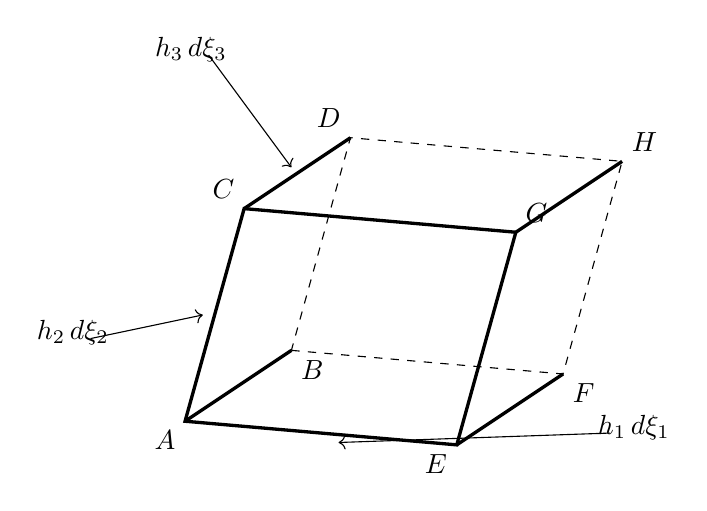
\begin{tikzpicture}[scale=1.5]
  % 曲面六面体：前面 A-E-G-C（实线），后面 B-F-H-D（虚线），深度棱 A-B、E-F、G-H、C-D（实线）
  \coordinate (A) at (1.3,0.6);
  \coordinate (E) at (3.6,0.4);
  \coordinate (G) at (4.1,2.2);
  \coordinate (C) at (1.8,2.4);
  \coordinate (B) at (2.2,1.2);
  \coordinate (F) at (4.5,1.0);
  \coordinate (H) at (5.0,2.8);
  \coordinate (D) at (2.7,3.0);
  % 背面（虚线）
  \draw[dashed] (B) -- (F) -- (H) -- (D) -- cycle;
  % 前面（实线）
  \draw[very thick] (A) -- (E) -- (G) -- (C) -- cycle;
  % 深度棱（实线）
  \draw[very thick] (A) -- (B) (E) -- (F) (G) -- (H) (C) -- (D);
  % 顶点标注
  \node[below left]  at (A) {$A$};
  \node[below left]  at (E) {$E$};
  \node[above right] at (G) {$G$};
  \node[above left]  at (C) {$C$};
  \node[below right] at (B) {$B$};
  \node[below right] at (F) {$F$};
  \node[above right] at (H) {$H$};
  \node[above left]  at (D) {$D$};
  % 拉梅系数标注（带引线箭头）
  \draw[->] (4.9,0.5) -- (2.6,0.42);
  \node at (5.1,0.55) {$h_1\, d\xi_1$};
  \draw[->] (0.5,1.3) -- (1.45,1.5);
  \node at (0.35,1.35) {$h_2\, d\xi_2$};
  \draw[->] (1.5,3.7) -- (2.2,2.75);
  \node at (1.35,3.75) {$h_3\, d\xi_3$};
\end{tikzpicture}
\par\vspace{2pt}
{\small 图 17.}
\end{figure}

\begin{figure}[htbp]
\centering
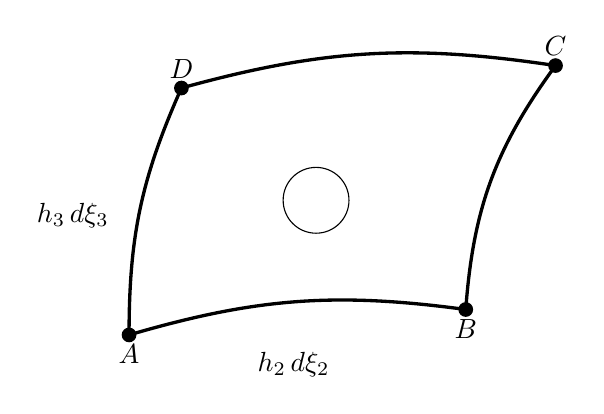
\begin{tikzpicture}[scale=1.9]
  % 曲边四边形 ABCD（ξ2ξ3 面）
  \coordinate (A) at (0.35,0.45);
  \coordinate (B) at (2.6,0.62);
  \coordinate (C) at (3.2,2.25);
  \coordinate (D) at (0.7,2.1);
  \draw[very thick] (A) to[bend left=12] (B) to[bend left=16] (C) to[bend right=12] (D) to[bend right=12] (A);
  \fill (A) circle (1.4pt) node[below]{$A$};
  \fill (B) circle (1.4pt) node[below]{$B$};
  \fill (C) circle (1.4pt) node[above]{$C$};
  \fill (D) circle (1.4pt) node[above]{$D$};
  % 线元标注
  \node[below] at (1.45,0.4) {$h_2\, d\xi_2$};
  \node[left] at (0.28,1.25) {$h_3\, d\xi_3$};
  % 内部空心圆
  \draw (1.6,1.35) circle (0.22);
\end{tikzpicture}
\par\vspace{2pt}
{\small 图 18.}
\end{figure}

\begin{equation*}
Q_1 = \frac{\partial}{\partial\xi_1} (A_1 h_2 h_3)\, d\xi_1\, d\xi_2\, d\xi_3.
\end{equation*}

类似地计算经过另外界面的流量差：

\begin{equation*}
Q_2 = \frac{\partial}{\partial\xi_2} (A_2 h_3 h_1)\, d\xi_1\, d\xi_2\, d\xi_3,
\end{equation*}

\begin{equation*}
Q_3 = \frac{\partial}{\partial\xi_3} (A_3 h_1 h_2)\, d\xi_1\, d\xi_2\, d\xi_3.
\end{equation*}

由此得到最后的结果：

\begin{equation*}
\nabla \cdot \ve{A} = \frac{1}{h_1 h_2 h_3} \left[ \frac{\partial}{\partial\xi_1} (h_2 h_3 A_1) + \frac{\partial}{\partial\xi_2} (h_1 h_3 A_2) + \frac{\partial}{\partial\xi_3} (h_1 h_2 A_3) \right].
\end{equation*}

例如，在球面坐标系中

\begin{equation*}
\operatorname{div}\ve{A} = \frac{1}{r^{2}}\, \frac{\partial (A_r r^{2})}{\partial r} + \frac{1}{r\sin\theta}\, \frac{\partial (A_\theta \sin\theta)}{\partial\theta} + \frac{1}{r\sin\theta}\, \frac{\partial A_\varphi}{\partial\varphi};
\end{equation*}

在柱面坐标系中

\begin{equation*}
\operatorname{div}\ve{A} = \frac{1}{\rho}\, \frac{\partial (\rho A_\rho)}{\partial\rho} + \frac{1}{\rho}\, \frac{\partial A_\varphi}{\partial\varphi} + \frac{\partial A_z}{\partial z}.
\end{equation*}

现考虑 $\operatorname{rot}\ve{A}$，它可用下面的方式确定：

\begin{equation*}
(\nabla \times \ve{A})_i = \lim_{S_i \to 0} \frac{1}{S_i} \oint \ve{A} \cdot d\ve{l}.
\end{equation*}

问题在于计算矢量 $\ve{A}$ 沿着图 18 上的闭围路 $ABCD$ 的环量。它等于四个被加项的代数和：

\begin{equation*}
\begin{aligned}
AB &\longrightarrow A_2 h_2\, d\xi_2 \big|_{\xi_3},\\
CD &\longrightarrow -A_2 h_2\, d\xi_2 \big|_{\xi_3 + d\xi_3},\\
BC &\longrightarrow A_3 h_3\, d\xi_3 \big|_{\xi_2 + d\xi_2},\\
DA &\longrightarrow -A_3 h_3\, d\xi_3 \big|_{\xi_2}.
\end{aligned}
\end{equation*}

因此
\begin{equation*}
\oint \ve{A} \cdot d\ve{l} = \left[-\frac{\partial}{\partial\xi_3} (A_2 h_2) + \frac{\partial}{\partial\xi_2} (A_3 h_3)\right] d\xi_2\, d\xi_3.
\end{equation*}

曲边四边形 $ABCD$ 的面积等于

\begin{equation*}
d\sigma_1 = h_2 h_3\, d\xi_2\, d\xi_3,
\end{equation*}

所以
\begin{equation*}
(\nabla \times \ve{A})_1 = \frac{1}{h_2 h_3} \left[ \frac{\partial}{\partial\xi_2} (A_3 h_3) - \frac{\partial}{\partial\xi_3} (A_2 h_2) \right],
\end{equation*}

类似地有：
\begin{equation*}
(\nabla \times \ve{A})_2 = \frac{1}{h_3 h_1} \left[ \frac{\partial}{\partial\xi_3} (A_1 h_1) - \frac{\partial}{\partial\xi_1} (A_3 h_3) \right],
\end{equation*}

\begin{equation*}
(\nabla \times \ve{A})_3 = \frac{1}{h_1 h_2} \left[ \frac{\partial}{\partial\xi_1} (A_2 h_2) - \frac{\partial}{\partial\xi_2} (A_1 h_1) \right].
\end{equation*}

例如，在球面坐标系中

\begin{equation*}
\operatorname{rot}_r \ve{A} = \frac{1}{r\sin\theta}\, \frac{\partial (A_\varphi \sin\theta)}{\partial\theta} - \frac{1}{r\sin\theta}\, \frac{\partial A_\theta}{\partial\varphi},
\end{equation*}

\begin{equation*}
\operatorname{rot}_\theta \ve{A} = \frac{1}{r\sin\theta}\, \frac{\partial A_r}{\partial\varphi} - \frac{1}{r}\, \frac{\partial (r A_\varphi)}{\partial r},
\end{equation*}

\begin{equation*}
\operatorname{rot}_\varphi \ve{A} = \frac{1}{r}\, \frac{\partial (r A_\theta)}{\partial r} - \frac{1}{r}\, \frac{\partial A_r}{\partial\theta};
\end{equation*}

在柱面坐标系中

\begin{equation*}
\operatorname{rot}_\rho \ve{A} = \frac{1}{\rho}\, \frac{\partial A_z}{\partial\varphi} - \frac{\partial A_\varphi}{\partial z},
\end{equation*}

\begin{equation*}
\operatorname{rot}_\varphi \ve{A} = \frac{\partial A_\rho}{\partial z} - \frac{\partial A_z}{\partial\rho},
\end{equation*}

\begin{equation*}
\operatorname{rot}_z \ve{A} = \frac{1}{\rho}\, \frac{\partial (\rho A_\varphi)}{\partial\rho} - \frac{1}{\rho}\, \frac{\partial A_\rho}{\partial\varphi}.
\end{equation*}


\chapter{$n$ 维空间中的线性代数}

\section{线性空间}

在数学和物理学中，经常会碰到一些相互之间可以相加以及与数相乘的那种对象。例如：齐次方程组的解，力学中的速度矢量，复数，以及在分析中已定义了加法和与数相乘运算的某个区间上的函数，等等。虽然这种对象与三维空间中的普通矢量在性质上可以毫无共同之处，但今后我们把这种对象仍然称为矢量。我们可将这种矢量的具体性质放在一边，而去寻求它的整体的固有规律性。而这里的“加法”和“乘法”运算已不必是通常意义下的那种加法和乘法，它们只须满足下面的条件即可：

\textbf{1. 加法} 对任意的矢量
\begin{flushleft}
$a$) $x + y = y + x,$

$b$) $(x + y) + z = x + (y + z)$ \hfill (2.1)

c) 存在矢量 $0$，使得 $x + 0 = x,$

d) 对任意矢量 $x$，存在矢量 $y$，使得 $x + y = 0$。
\end{flushleft}

\textbf{2. 乘法} 如果 $x, y$ 是矢量，而 $\alpha, \beta$ 是数，则

$a$) $1 \cdot x = x$

\begin{equation*}
\text{b)}\ \ \alpha \cdot (\beta x) = (\alpha \beta) \cdot x,\tag{2.2}
\end{equation*}

\begin{equation*}
\begin{array}{r l} \mathbf {c}) & (\alpha + \beta) (x + y) = \alpha (x + y) + \beta (x + y) = \\ & = \alpha x + \alpha y + \beta x + \beta y. \end{array}
\end{equation*}

集 $X$ ，如果对它的元素(称为矢量)可引进如下的加法和乘法运算，则此集 $X$ 称为线性空间：

1）满足条件(2.1)的，且由此集的两个元素 $x_{1}$ ， $x_{2}$ 能构造此集中的第三个元素 $x_{3}$ 作为它们的“和”的加法运算；

2）满足条件(2.2)的，且由此集的任一元素 $x$ 和任一数 $\alpha$ ，可构造此集的新元素 $\alpha x$ 的乘法运算。

开始时可能以为这种抽象的定义仅对数学有用，而在研究物理问题时未必有效。但事实上线性空间的概念是许多数学分支的基础，它在物理学中的应用也有重大的价值。为了阐明线性空间的概念，我们举一些例子。

\textbf{例 1}\quad 通常的三维空间：服从矢量加法法则的普通矢量，是此空间的元素。不难验证，矢量间的加法运算和矢量与数的乘法运算，满足条件(2.1)和(2.2)。因此，三维空间是线性空间。

\textbf{例 2}\quad 以 $n$ 个实数构成的有序集 $x = (\xi_{1}, \xi_{2}, \cdots, \xi_{n})$ 为元素的空间。其中数 $\xi_{i}$ 称为矢量 $x$ 的第 $i$ 个坐标。对这种矢量的加法运算和乘法运算定义如下：

\begin{equation*}
\begin{array}{r l} & (\xi_ {1}, \xi_ {2}, \dots , \xi_ {n}) + (\eta_ {1}, \eta_ {2}, \dots , \eta_ {n}) = \\ & = (\xi_ {1} + \eta_ {1}, \xi_ {2} + \eta_ {2}, \dots , \xi_ {n} + \eta_ {n}), \\ & \alpha (\xi_ {1}, \xi_ {2}, \dots , \xi_ {n}) = (\alpha \xi_ {1}, \alpha \xi_ {2}, \dots , \alpha \xi_ {n}). \end{array}
\end{equation*}

不难验证，用这种方式定义的加法和乘法运算，满足公理(2.1)和(2.2)，所以此空间是线性空间。

\textbf{例 3}\quad 定义在区间 $a \leqslant t \leqslant b$ 上的连续函数 $f(t)$ 也可取作线性空间的元素，其加法和乘法与分析中所讲的一样。

现在引进矢量的线性相关这一重要概念。假定 $x_{1}, x_{2}, \cdots, x_{n}$ 为线性空间$R$内的$n$个矢量，而 $a_{1}, a_{2}, \cdots, a_{n}$ 是数。

如果等式
\begin{equation*}
\sum_ {i = 1} ^ {n} a _ {i} x _ {i} = 0\tag{2.3}
\end{equation*}

当且仅当所有 $a_{i}$ 等于零时才成立，则矢量 $x_{1}, x_{2}, \cdots, x_{n}$ 称为线性无关。在相反的情形，就称矢量 $x_{1}, x_{2}, \cdots, x_{n}$ 线性相关。

如果 $x = \sum_{i=1}^{n} a_{i} x_{i}$ ，则称矢量 $x$ 为矢量 $x_{1}, x_{2}, \cdots, x_{n}$ 的线性组合。如果矢量 $x_{1}, x_{2}, \cdots, x_{n}$ 线性相关，则其中至少有一个是其余的线性组合。

\textbf{例 4}\quad 三维空间中三个互不共面的矢量线性无关。

\textbf{例 5}\quad 今证 $k+1$ 个函数 $1, t, t^{2}, \cdots, t^{k}$ 线性无关。因若不然，则有

\begin{equation*}
a _ {0} \cdot 1 + a _ {1} t + \dots + a _ {k} t ^ {k} = 0,\tag{2.4}
\end{equation*}

这里 $a_{0}, a_{1}, \cdots, a_{k}$ 不全为零。将等式(2.4)逐次微分 $k$ 次，就得 $k + 1$ 个方程组。因为此方程组的系数行列式不为零，故解之得

\begin{equation*}
a _ {0} = a _ {1} = \dots = a _ {k} = 0.
\end{equation*}

这就证明了矢量 $1, t, t^{2}, \cdots, t^{k}$ 在函数空间中线性无关。

设 $\{e_{1}, e_{2}, \cdots, e_{n}\}$ 为空间 $R$ 中的线性无关组。如果 $R$ 中的任一矢量都可表示为这些矢量的线性组合，即：

\begin{equation*}
x = \sum_ {i = 1} ^ {n} \eta_ {i} e _ {i},\tag{2.5}
\end{equation*}

则 $\{e_{1}, e_{2}, \cdots, e_{n}\}$ 就称为线性空间的基。

展开式(2.5)中的系数是唯一确定的。因对同一个矢量如有二种展开式，即

\begin{equation*}
x = \sum_ {i = 1} ^ {n} \xi_ {i} e _ {i} = \sum_ {i = 1} ^ {n} \eta_ {i} e _ {i},
\end{equation*}

则从一个展开式减去另一个，就得等式

\begin{equation*}
\sum_ {i = 1} ^ {n} \left(\xi_ {i} - \eta_ {i}\right) e _ {i} = 0,
\end{equation*}

这里 $(\xi_{i}-\eta_{i})$ 不全为零。但这是不可能的，因 $e_{i}$ 线性无关。 $(\eta_{1},\eta_{2},\cdots,\eta_{n})$ 就叫做矢量$x$在基 $\{e_{1},e_{2},\cdots,e_{n}\}$ 中的坐标。

\textbf{例 6}\quad 三个互相垂直的矢量就给了三维空间中的一个基。在这种情形，矢量的坐标就是它在基矢量上的投影。

\textbf{例 7}\quad 在每个元素是由 $n$ 个数构成的有序集的空间中，矢量 $e_{1}=(1,0,\cdots,0)$ ， $e_{2}=(0,1,\cdots,0)$ ， $\cdots$ ， $e_{n}=(0,0,\cdots,0,1)$ 为它的基矢量。这是因为任一矢量 $x$ 都可表示成

\begin{equation*}
x = \sum_ {i = 1} ^ {n} \eta_ {i} e _ {i}.
\end{equation*}

现引进空间维数的概念。如果在线性空间中存在 $n$ 个线性无关的矢量，但不可能找出 $n+1$ 个线性无关的矢量，则此空间就称为 $n$ 维空间。而 $n$ 就称为此空间的维数。在 $n$ 维空间中必定存在由 $n$ 个线性无关的矢量构成的基，并且任意一组 $n$ 个线性无关的矢量都能作为 $n$ 维空间的基。

\textbf{例 8}\quad 元素为 $n$ 个数构成的有序集的空间，是 $n$ 维的。

前例中所举的 $n$ 个矢量构成了它的基。

\textbf{例 9}\quad 函数空间是无限维的，即线性无关的矢量的个数可任意多。此时上面所定义的那种意义的基，在函数空间中就不存在了。

\section{矩阵及其运算}

由一些数组成的矩形表，称为矩阵。矩阵通常用下面的记号表示：

\begin{equation*}
\| a _ {i j} \| = A = \left[ \begin{array}{c c c c} a _ {1 1} & a _ {1 2} & \dots & a _ {1 n} \\ a _ {2 1} & a _ {2 2} & \dots & a _ {2 n} \\ \dots & \dots & \dots & \dots \\ a _ {m 1} & a _ {m 2} & \dots & a _ {m n} \end{array} \right] \cdot
\end{equation*}

矩阵中分布在同一水平线上的那些元素全体，叫做它的行；在同一垂直线上的，叫做它的列。矩阵元素 $a_{ij}$ 的第一和第二个下标分别指出了这个元素所在位置的行和列的号码。可以引进矩阵相加和矩阵与数相乘的运算法则。

一矩阵，它的下标为 $i$ 和 $j$ 的元素等于矩阵 $A$ 和 $B$ 具有相同下标的元素之和，则此矩阵就称为矩阵 $A$ 和 $B$ 的和。

一矩阵，它的下标为 $i$ 和 $j$ 的元素等于矩阵 $A$ 中具有相同下标的元素与数 $\lambda$ 的积，则此矩阵就称为矩阵 $A$ 与数相乘的积。

不难验证，用这种方法定义的运算，分别满足条件(2.1)和(2.2)。因此，$m$ 行和 $n$ 列矩阵的集合成为一线性空间。

这种空间的基由下述矩阵构成：在这种矩阵中仅有一个元素等于1，而其余元素等于零。同时，等于1的元素的下标跑遍所有可能的值，即基矩阵为

\begin{equation*}
\left[ \begin{array}{c c c c c} 1 & 0 & 0 & \dots & 0 \\ 0 & 0 & 0 & \dots & 0 \\ \dots & \dots & \dots & \dots & \dots \\ 0 & 0 & 0 & \dots & 0 \end{array} \right], \quad \left[ \begin{array}{c c c c c} 0 & 1 & 0 & \dots & 0 \\ 0 & 0 & 0 & \dots & 0 \\ \dots & \dots & \dots & \dots & \dots \\ 0 & 0 & 0 & \dots & 0 \end{array} \right] \dots \left[ \begin{array}{c c c c c} 0 & 0 & 0 & \dots & 1 \\ 0 & 0 & 0 & \dots & 0 \\ \dots & \dots & \dots & \dots & \dots \\ 0 & 0 & 0 & \dots & 0 \end{array} \right],
\end{equation*}

\begin{equation*}
\left[ \begin{array}{c c c c c} 0 & 0 & 0 & \dots & 0 \\ 1 & 0 & 0 & \dots & 0 \\ \dots & \dots & \dots & \dots & \dots \\ 0 & 0 & 0 & \dots & 0 \end{array} \right], \quad \left[ \begin{array}{c c c c c} 0 & 0 & 0 & \dots & 0 \\ 0 & 1 & 0 & \dots & 0 \\ \dots & \dots & \dots & \dots & \dots \\ 0 & 0 & 0 & \dots & 0 \end{array} \right] \dots \left[ \begin{array}{c c c c c} 0 & 0 & 0 & \dots & 0 \\ 0 & 0 & 0 & \dots & 1 \\ \dots & \dots & \dots & \dots & \dots \\ 0 & 0 & 0 & \dots & 0 \end{array} \right],
\end{equation*}

\begin{equation*}
\left[ \begin{array}{c c c c c} 0 & 0 & 0 & \dots & 0 \\ 0 & 0 & 0 & \dots & 0 \\ \dots & \dots & \dots & \dots \\ 1 & 0 & 0 & \dots & 0 \end{array} \right], \quad \left[ \begin{array}{c c c c c} 0 & 0 & 0 & \dots & 0 \\ 0 & 0 & 0 & \dots & 0 \\ \dots & \dots & \dots & \dots \\ 0 & 1 & 0 & \dots & 0 \end{array} \right] \dots \left[ \begin{array}{c c c c c} 0 & 0 & 0 & \dots & 0 \\ 0 & 0 & 0 & \dots & 0 \\ \dots & \dots & \dots & \dots \\ 0 & 0 & 0 & \dots & 1 \end{array} \right].
\end{equation*}

不难看出，基矩阵的个数等于 $m \times n$ ；因此，矩阵空间的维数也等于 $m \times n$ 。

除了加法和与数相乘的运算外，对矩阵还可引进其他一些运算。

设有一个 $m$ 行 $n$ 列矩阵 $A$ 和另一个 $n$ 行 $l$ 列矩阵 $B$。我们将 $A$ 的第 $i$ 行元素与 $B$ 的第 $j$ 列元素依次对应相乘，然后再相加，得

\begin{equation*}
(A B) _ {i j} = \sum_ {k = 1} ^ {n} A _ {i k} B _ {k j} \quad \left\{ \begin{array}{l} i = 1, 2, \dots , m, \\ j = 1, 2, \dots , l. \end{array} \right.\tag{2.6}
\end{equation*}

以 $(AB)_{ij}$ 作为一新矩阵位于第 $i$ 行、第 $j$ 列交叉处的元素，则这个 $m$ 行 $l$ 列矩阵就称为矩阵 $A$ 和 $B$ 的积。

这样一来，矩阵之积仅当矩阵 $A$ 的列数与 $B$ 的行数相等时，才有定义。

将矩阵 $A$ 的行变为列(号码不变)，得一矩阵，此矩阵就称为关于 $A$ 的转置，并用记号 $\widetilde{A}$ 表示。换言之，矩阵 $\widetilde{A}$ 位于第 $i$ 行和第 $j$ 列相交处的元素 $\widetilde{A}_{ij}$ 由下面的方法确定：

\begin{equation*}
(\widetilde {A}) _ {i j} = A _ {j i}.
\end{equation*}

如果矩阵 $A$ 有 $m$ 行和 $n$ 列，则 $\widetilde{A}$ 就有 $n$ 行和 $m$ 列。

矩阵 $A$ 的复共轭矩阵 $A^{*}$ 可这样作出： $A^{*}$ 的下标为 $i$, $j$ 的元素，其值为原矩阵 $A$ 的下标为 $i$, $j$ 的元素的复共轭：

\begin{equation*}
(A ^ {*}) _ {i j} = A _ {i j} ^ {*}.
\end{equation*}

矩阵 $A$ 通过转置再加复共轭后所得的矩阵 $A^{+}$ 称为 $A$ 的厄米 (Hermite) 共轭矩阵：

\begin{equation*}
(A ^ {+}) _ {i j} = (A _ {j i}) ^ {*}.
\end{equation*}

如果 $A$ 是 $m$ 行 $n$ 列矩阵，则 $A^{+}$ 是 $n$ 行 $m$ 列矩阵。

现将上述运算的最重要的性质列举如下：

1. 矩阵乘法的结合律。即

\begin{equation*}
(A B) C = A (B C)\tag{2.7}
\end{equation*}

事实上
\begin{equation*}
\begin{array}{r l} {[ (A B) C ] _ {i j} = \sum_ {k} (A B) _ {i k} C _ {k j} = \sum_ {e, k} A _ {i e} B _ {e k} C _ {k j} =} & \\ {= \sum_ {e} A _ {i e} (B C) _ {e j} = [ A (B C) ] _ {i j}.} \end{array}
\end{equation*}

2. 对于转置矩阵的积，则成立下面的关系：

\begin{equation*}
\widetilde {A B} = \widetilde {B} \widetilde {A},\tag{2.8}
\end{equation*}

事实上
\begin{equation*}
\begin{array}{r l} (\widetilde {A B}) _ {i j} & = (A B) _ {j i} = \sum_ {k} A _ {j k} B _ {k i} \\ & = \sum_ {k} \widetilde {A} _ {k j} \widetilde {B} _ {i k} = (\widetilde {B} \widetilde {A}) _ {i j}. \end{array}
\end{equation*}

3. 矩阵的乘法不可交换。即

\begin{equation*}
A B \neq B A.
\end{equation*}

注意，因矩阵之积仅在下述情形才有定义，即相乘矩阵中的第一个矩阵的列数等于第二个矩阵的行数，而不必要求第二个矩阵的列数等于第一个的行数。所以一般说来，$B$与$A$的积是不一定有意义的。

如果
\begin{equation*}
A B = B A,
\end{equation*}

便称两矩阵对乘法是可交换的；在相反的情形，两矩阵就称为对乘法是不可交换的。

4. 对于复共轭矩阵，则有下面的关系：

\begin{equation*}
(A B) ^ {*} = A ^ {*} B ^ {*}\tag{2.9}
\end{equation*}

5. 对于厄米共轭矩阵，满足等式

\begin{equation*}
(A B) ^ {+} = B ^ {+} A ^ {+}\tag{2.10}
\end{equation*}

等式(2.9)和(2.10)的正确性，可用初等的方法加以验证。

以后我们用大写的拉丁字母表示方阵（即行数与列数相等的矩阵），例如

\begin{equation*}
A = \left[ \begin{array}{c c c c} a _ {1 1} & a _ {1 2} & \dots & a _ {1 n} \\ a _ {2 1} & a _ {2 2} & \dots & a _ {2 n} \\ \dots & \dots & \dots & \dots \\ a _ {n 1} & a _ {n 2} & \dots & a _ {n n} \end{array} \right];
\end{equation*}

而用小写字母 $x$、$y$、$z$、 $\varphi$ 、 $\psi$ 等表示仅有一列的矩阵，例如

\begin{equation*}
x = \left[ \begin{array}{c} x _ {1} \\ x _ {2} \\ \vdots \\ x _ {n} \end{array} \right].
\end{equation*}

显然，只含一行的矩阵只需用同样的字母，再加上表示转置记号～即可，例如

\begin{equation*}
\widetilde {x} = \left(x _ {1}, x _ {2}, \dots , x _ {n}\right).
\end{equation*}

我们将把列 $x$ 简称为 $n$ 维空间的矢量(参看本章的例 2)。

还需注意一个特殊情形。主对角线上的元素都为 1，而其余元素为 0 的矩阵称为单位矩阵。对于它，我们用特别的记号表示：

\begin{equation*}
I = \left[ \begin{array}{c c c c} 1 & 0 & \dots & 0 \\ 0 & 1 & \dots & 0 \\ \dots & \dots & \dots & \dots \\ 0 & 0 & \dots & 1 \end{array} \right] \quad (I) _ {i j} = \delta_ {i j}.
\end{equation*}

由关于矩阵运算和单位矩阵的定义，可直接推出下列等式的正确性：

\begin{equation*}
\begin{array}{c} I A = A I, \\ I = I ^ {*} = \widetilde {I} = I ^ {+}. \end{array}
\end{equation*}

有关矩阵的行列式的概念，假定读者是熟知的。此外，我们还不加证明地引进几个结果，这些都可在代数学中找到。\textcircled{1}

\textbf{1. 等式}

\begin{equation*}
\sum_ {j = 1} ^ {n} A _ {i j} x _ {j} = 0 (i = 1, 2, \dots , n)\tag{2.11}
\end{equation*}

仅在 $\operatorname{det}|A| = 0$ 或所有 $x_{j} = 0$ 的条件下才成立。

\textbf{2. 由等式}

\begin{equation*}
A B = 0\tag{2.12}
\end{equation*}

及
\begin{equation*}
\det | A | \neq 0\tag{2.13}
\end{equation*}

推出
\begin{equation*}
B = 0.\tag{2.14}
\end{equation*}

3. 对于任一非零矢量 $y$ 和行列式不为零的矩阵 $A$ ，总可找到这样的非零矢量 $x$ ，使得等式

\begin{equation*}
A x = y\tag{2.15}
\end{equation*}

成立。

4. 两个矩阵积的行列式等于这些矩阵行列式的积，即

\begin{equation*}
\det | A B | = \det | A | \cdot \det | B |.\tag{2.16}
\end{equation*}

矩阵 $B$ 称为 $A$ 的逆矩阵，如果

\begin{equation*}
A B = I,\tag{2.17}
\end{equation*}

这里 $I$ 是单位矩阵。矩阵 $A$ 的逆矩阵用 $A^{-1}$ 表示。

\textbf{定理 2.1}\quad 任一行列式不等于零的矩阵都存在逆矩阵。

\textbf{证明}\quad 考虑行列式不等于零的矩阵 $A$ 。由(2.15)，总可找到这样的矢量 $x^j$ ，使得

\begin{equation*}
A x ^ {j} = A \left[ \begin{array}{c} x _ {1} ^ {j} \\ x _ {2} ^ {j} \\ \vdots \\ x _ {n} ^ {j} \end{array} \right] = \left[ \begin{array}{c} 0 \\ 0 \\ \vdots \\ 1 \\ \vdots \\ 0 \end{array} \right] = e _ {j},
\end{equation*}

这里 $e_{j}$ 为第 $j$ 个分量为1，而其余为零的矢量。

现考虑第 $j$ 列是矢量 $x^{j}$ 的矩阵，即矩阵

\begin{equation*}
\left[ \begin{array}{c c c c} x _ {1} ^ {1} & x _ {1} ^ {2} & \dots & x _ {1} ^ {n} \\ x _ {2} ^ {1} & x _ {2} ^ {2} & \dots & x _ {2} ^ {n} \\ \dots & \dots & \dots & \dots \\ x _ {n} ^ {1} & x _ {n} ^ {2} & \dots & x _ {n} ^ {n} \end{array} \right],
\end{equation*}

并记此矩阵为 $A^{-1}$ 。显然

\begin{equation*}
A A ^ {- 1} = \left[ \begin{array}{c c c c} 1 & 0 & \dots & 0 \\ 0 & 1 & \dots & 0 \\ \dots & \dots & \dots & \dots \\ 0 & 0 & \dots & 1 \end{array} \right] = I.
\end{equation*}

现在，为得定理的结果，只需再作下面很明显的变换：

\begin{equation*}
\begin{array}{l} A A ^ {- 1} A = I A = A I, \\ A (A ^ {- 1} A - I) = 0. \end{array}
\end{equation*}

但因 $\operatorname{det}|A| \neq 0$ ，故由(2.14)

\begin{equation*}
A ^ {- 1} A - I = 0,
\end{equation*}

或
\begin{equation*}
A ^ {- 1} A = I.
\end{equation*}

这就是所要证明的。

满足条件
\begin{equation*}
U ^ {+} U = I,
\end{equation*}

即
\begin{equation*}
\sum_ {k} U _ {i k} ^ {+} U _ {k j} = \sum_ {k} U _ {k i} ^ {*} U _ {k j} = \delta_ {i j}\tag{2.18}
\end{equation*}

的矩阵称为酉矩阵。

\textbf{定理 2.2}\quad 如果

\begin{equation*}
\det | U ^ {*} U | = 1,\tag{2.19}
\end{equation*}

则
\begin{equation*}
\det | U | = e ^ {i \bar {\varphi}}\tag{2.20}
\end{equation*}

这里 $\varphi$ 是实数。

\textbf{证明}\quad 等式

\begin{equation*}
\det | A | = \det | \widetilde {A} |\tag{2.21}
\end{equation*}

可由行列式的性质直接推出。利用(2.21)，易知下面的等式成立：

\begin{equation*}
\det | A ^ {+} | = \det | A ^ {*} | = (\det | A |) ^ {*}.\tag{2.22}
\end{equation*}

其次，利用(2.16)将(2.19)写成

\begin{equation*}
\det | U ^ {*} U | = \det | U ^ {*} | \det | U | = 1.\tag{2.23}
\end{equation*}

现在显然
\begin{equation*}
\det | U ^ {*} | \det | U | = | \det | U | | ^ {2} = 1,\tag{2.24}
\end{equation*}

由此直接推出(2.20)。

注意，在定理2.2中，将 $U^{*}$ 改作 $U^{+}$ ，结论仍然成立，因为

\begin{equation*}
\det | U ^ {+} | = \det | U ^ {*} |\tag{2.25}
\end{equation*}

附注：对酉矩阵，等式(2.19)成立。但等式(2.19)的成立还不足以表明 $U$ 是酉矩阵。例如

\begin{equation*}
U = \left( \begin{array}{c c} 1 & 1 \\ 1 & 2 \end{array} \right).
\end{equation*}

\textbf{定理 2.3}\quad 如果 $U$ 是酉矩阵，则由等式

\begin{equation*}
x ^ {\prime} = U x\tag{2.26}
\end{equation*}

可推出
\begin{equation*}
\left(x ^ {\prime}\right) ^ {+} = x ^ {+} U ^ {+}, \quad \left(x ^ {\prime}\right) ^ {+} x ^ {\prime} = x ^ {+} x.\tag{2.27}
\end{equation*}

\textbf{证明}\quad 对(2.26)施行共轭运算，则得

\begin{equation*}
(x ^ {\prime}) ^ {+} = x ^ {+} U ^ {+},\tag{2.28}
\end{equation*}

将(2.26)和(2.28)相乘，即得

\begin{equation*}
\left(x ^ {\prime}\right) ^ {+} x ^ {\prime} = x ^ {+} U ^ {+} U x = x ^ {+} I x = x ^ {+} x,
\end{equation*}

这就是所要证明的。

\textbf{定理 2.4}\quad 如果

\begin{equation*}
x ^ {\prime} = V x,\tag{2.29}
\end{equation*}

则等式
\begin{equation*}
\tilde {x} ^ {\prime} x ^ {\prime} = \tilde {x} x\tag{2.30}
\end{equation*}

当且仅当条件

\begin{equation*}
\widetilde {V} V = V \widetilde {V} = I\tag{2.31}
\end{equation*}

满足时才成立。

\textbf{证明}\quad 充分性。对(2.29)施行转置运算，

\begin{equation*}
\tilde {x} ^ {\prime} = \tilde {x} \tilde {V}.\tag{2.32}
\end{equation*}

将(2.32)和(2.29)相乘，得

\begin{equation*}
\widetilde {x} ^ {\prime} x ^ {\prime} = \widetilde {x} \widetilde {V} V x = \widetilde {x} I x = \widetilde {x} x;
\end{equation*}

条件(2.31)的充分性证毕。

必要性。设 $x$ 是单位矢量 $e_{i}$ ，即

\begin{equation*}
x = \left[ \begin{array}{c} 0 \\ 0 \\ \vdots \\ 1 \\ \vdots \\ 0 \end{array} \right].\tag{2.33}
\end{equation*}

如果 $\widetilde{x}^{\prime}x^{\prime} = \widetilde{x} x$ ，则

\begin{equation*}
\begin{array}{r l} \widetilde {x} ^ {\prime} x ^ {\prime} - \widetilde {x} x & = 0 = \widetilde {x} \widetilde {V} V x - \widetilde {x} x = \\ & = \widetilde {x} (\widetilde {V} V - I) x. \end{array}\tag{2.34}
\end{equation*}

由(2.34)和(2.33)推出

\begin{equation*}
(\widetilde {V} V - I) _ {i i} = 0.\tag{2.35}
\end{equation*}

现设 $\widetilde{x}$ 是第 $i$ 和第 $j$ 两个坐标等于1，其余坐标等于0的矢量：

\begin{equation*}
\widetilde {x} = (0 0 \dots 1 0 \dots 0 1 \dots 0).\tag{2.36}
\end{equation*}

将(2.36)代入(2.34)，有

\begin{equation*}
\begin{array}{r l} & (\widetilde {V} V - I) _ {i j} + (\widetilde {V} V - I) _ {i i} + (\widetilde {V} V - I) _ {j i} + \\ & \quad + (\widetilde {V} V - I) _ {j j} = 0. \end{array}
\end{equation*}

由此并注意到等式(2.35)，就得

\begin{equation*}
(\widetilde {V} V - I) _ {i j} + (\widetilde {V} V - I) _ {j i} = 0,
\end{equation*}

或
\begin{equation*}
(\widetilde {V} V - I) _ {i j} = - (\widetilde {V} V - I) _ {j i} = - (\widetilde {V} V - I) _ {i j};
\end{equation*}

所以
\begin{equation*}
\widetilde {V} V - I = 0.
\end{equation*}

因为 $\widetilde{V} V = I$ ，注意到(2.21)，就得

\begin{equation*}
\det | \widetilde {V} V | = (\det | V |) ^ {2} = \det | I | = 1;
\end{equation*}

所以
\begin{equation*}
\det \left| V \right| = \pm 1.
\end{equation*}

因此，如果
\begin{equation*}
\widetilde {V} V = I,
\end{equation*}

则也有
\begin{equation*}
V \widetilde {V} = I,
\end{equation*}

这就是所要证明的。

满足条件(2.31)的矩阵称为正交矩阵。

\textbf{例 10}\quad 在二维实空间中，正交矩阵有下面的形式：

1) 当 $\operatorname{det}|V| = 1$ 时，

\begin{equation*}
V = \left( \begin{array}{c c} \cos \varphi & \sin \varphi \\ - \sin \varphi & \cos \varphi \end{array} \right),\tag{2.37}
\end{equation*}

2) 当 $\operatorname{det}|V| = -1$ 时，

\begin{equation*}
V = \left( \begin{array}{c c} \cos \varphi & \sin \varphi \\ \sin \varphi & - \cos \varphi \end{array} \right);\tag{2.38}
\end{equation*}

在这两种情形，都是

\begin{equation*}
\varphi = v + i w,
\end{equation*}

这里 $v$ 和 $w$ 是实数。矩阵(2.37)和(2.38)的正交性，不难直接加以验证。

现证明，所有满足条件

\begin{equation*}
\widetilde {V} V = I\tag{2.39}
\end{equation*}

的二阶矩阵都有(2.37)或(2.38)的形式。事实上，矩阵方程(2.39)等价于下面的方程组：

\begin{equation*}
\begin{array}{l} V _ {1 1} ^ {2} + V _ {1 2} ^ {2} = 1, \\ V _ {1 1} V _ {2 1} + V _ {1 2} V _ {2 2} = 0, \\ V _ {2 1} ^ {2} + V _ {2 2} ^ {2} = 1. \end{array}\tag{2.40}
\end{equation*}

设 $\varphi = \operatorname{arc}\cos V_{11}$ ，则由(2.40)得

\begin{equation*}
\begin{array}{l l} V _ {1 2} = \sin \varphi , & \frac {V _ {2 1}}{V _ {2 2}} = - \frac {\sin \varphi}{\cos \varphi}, \\ V _ {2 1} = \pm \sin \varphi , & V _ {2 2} = \mp \cos \varphi . \end{array}
\end{equation*}

这就是所要证明的。

\textbf{定理 2.5}\quad 如果 $V_{1}$ 和 $V_{2}$ 是正交矩阵，则 $V_{1}V_{2}$ 也是正交矩阵。类似地，如果 $U_{1}$ 和 $U_{2}$ 是酉矩阵，则 $U_{1}U_{2}$ 也是酉矩阵。

\begin{equation*}
\begin{array}{r l} \text {证明} & (\widetilde {V _ {1} V _ {2}}) (V _ {1} V _ {2}) = \widetilde {V} _ {2} \widetilde {V} _ {1} V _ {1} V _ {2} = \\ & = \widetilde {V} _ {2} V _ {2} = I. \end{array}
\end{equation*}

完全同样地
\begin{equation*}
\left(U _ {1} U _ {2}\right) ^ {+} \left(U _ {1} U _ {2}\right) = U _ {2} ^ {+} U _ {1} ^ {+} U _ {1} U _ {2} = U _ {2} ^ {+} U _ {2} = I.
\end{equation*}

\section{线性算子}

如果在 $n$ 维空间中给了一个法则 $A$ ，根据这个法则，对此空间中的任一矢量 $x$ ，都能有此空间中的矢量 $y$ 与之对应，则我们就称在此空间中给定了算子 $A$ ，并将 $y$ 记为

\begin{equation*}
y = A x.
\end{equation*}

如果算子 $A$ 还满足下面两个条件：

\begin{equation*}
1) A (x _ {1} + x _ {2}) = A x _ {1} + A x _ {2},
\end{equation*}

\begin{equation*}
2) A (\lambda x) = \lambda A x.
\end{equation*}

则称算子 $A$ 为线性算子。

\textbf{例11}\quad 考虑算子 $I$ ，它使矢量 $\pmb{x}$ 与它本身相对应：

\begin{equation*}
I x = x.
\end{equation*}

这个算子称为单位算子或恒等算子。易见，单位算子是线性的。

\textbf{例 12}\quad 将线性空间中任一矢量都变为零矢量的算子, 称为零算子:

\begin{equation*}
O x = 0.
\end{equation*}

\textbf{例13}\quad 考虑每个元素是形如

\begin{equation*}
x = (\xi_ {1}, \xi_ {2}, \dots , \xi_ {n})
\end{equation*}

的线性空间，其次假定 $A$ 是有 $\pmb{n}$ 行的方阵，

\begin{equation*}
A = \left\| a _ {i k} \right\| \quad (i, k = 1, 2, \dots , n).
\end{equation*}

现用下式定义算子 $A$

\begin{equation*}
A x = \parallel a _ {i k} \parallel x,\tag{2.41}
\end{equation*}

这里右边的表示式理解为矩阵乘以矢量，这说明，算子 $A$ 作用于矢量 $x$ 后所得的矢量，等于矢量 $x$ 左乘以矩阵 $\|a_{ik}\|$ 所得的结果。于是矢量 $Ax$ 的分量可由下式确定：

\begin{equation*}
\eta_ {i} = \sum_ {k = 1} ^ {n} a _ {i k} \xi_ {k} \quad (i = 1, 2, \dots , n).
\end{equation*}

显然这种算子是线性的。

对于线性算子，当然也可以定义加法和与数的乘法运算。

算子 $C$ 称为线性算子 $A$ 和 $B$ 的和，如果它使 $\pmb{n}$ 维空间中的任一矢量 $x$ ，对应矢量 $Ax + Bx$ ，即用等式

\begin{equation*}
C x = A x + B x\tag{2.42a}
\end{equation*}

来定义线性算子的加法运算

\begin{equation*}
C = A + B.
\end{equation*}

由给出算子 $A$ 和 $B$ 的线性空间中加法的可结合性和可交换性，可推知算子 $A$ 和 $B$ 的加法也具有可结合性和可交换性。容易验证，算子的加法对(2.1)中其余的条件也满足。

一算子称为算子 $A$ 与数 $\lambda$ 的积，如果它将矢量 $x$ 变为矢量 $\lambda(Ax)$ 。这样，由定义

\begin{equation*}
\lambda A x = \lambda (A x).\tag{2.42b}
\end{equation*}

算子与数相乘的运算满足条件(2.2)。

这样一来，在线性空间上的线性算子的全体也构成一个线性空间。由此也知对任一线性算子 $A$ ，存在这样的算子 $(-A)$ ，使得

\begin{equation*}
A + (- A) = 0.
\end{equation*}

现在显然，由(2.41)，每个矩阵都定义了某个线性算子，故矩阵集合本身也构成了线性空间。下面的定理建立了矩阵和线性算子之间的联系。

\textbf{定理 2.6}\quad 在基给定时，每一个线性算子都有一个确定的矩阵与之对应。反之亦真，即在固定基下，每个矩阵都对应于某个线性算子。

\textbf{证明}\quad 分两步进行。先证明，存在唯一的线性算子，把 $n$ 维空间中的 $n$ 个基矢量 $e_1, e_2, \cdots, e_n$ 变为同一空间中预先给定的 $n$ 个矢量 $f_1, f_2, \cdots, f_n$ 。此后，在矩阵和算子之间建立一一对应关系就不难了。

即要证明，总存在唯一的线性算子 $A$ ，对于它，下面等式成立：

\begin{equation*}
A e _ {1} = f _ {1}, \quad A e _ {2} = f _ {2}, \quad \dots , \quad A e _ {n} = f _ {n}.\tag{2.43}
\end{equation*}

先证实,这样的算子可用 $n$ 个矢量 $f_{1}$ , $f_{2}$ , $\cdots$ , $f_{n}$ 唯一地确定。设

\begin{equation*}
x = \eta_ {1} e _ {1} + \eta_ {2} e _ {2} + \dots + \eta_ {n} e _ {n};
\end{equation*}

则
\begin{equation*}
\begin{array}{r l} A x & = A \left(\eta_ {1} e _ {1} + \eta_ {2} e _ {2} + \dots + \eta_ {n} e _ {n}\right) = \\ & = \eta_ {1} A e _ {1} + \eta_ {2} A e _ {2} + \dots + \eta_ {n} A e _ {n} = \\ & = \eta_ {1} f _ {1} + \eta_ {2} f _ {2} + \dots + \eta_ {n} f _ {n}. \end{array}
\end{equation*}

因此，Ax 可用 $n$ 个矢量 $f_{1}$ ， $f_{2}$ ，…， $f_{n}$ 唯一地确定。

现证明，对任意的 $n$ 个矢量 $f_{1}, f_{2}, \cdots, f_{n}$ 存在用 (2.43) 式确定的算子 $A$。为此，将矢量 $e_{i}$ 对应于矢量 $f_{i} (i = 1, 2, \cdots, n)$ ，于是矢量

\begin{equation*}
x = \sum_ {i = 1} ^ {n} \eta_ {i} e _ {i}
\end{equation*}

可对应于矢量

\begin{equation*}
A x = \sum_ {i = 1} ^ {n} \eta_ {i} A e _ {i}.
\end{equation*}

因矢量 $x$ 可用自己的坐标完全确定，故它(即 $x$ )所对应的矢量 $Ax$ 也将完全确定。

算子 $A$ 的线性性质是不难验证的。这样，我们就完成了证明的第一步。

将矢量 $f_{i}$ 表示成 $n$ 个基矢量 $e_{1}, e_{2}, \cdots, e_{n}$ 的线性组合：

\begin{equation*}
f _ {i} = A e _ {i} = \sum_ {j = 1} ^ {n} a _ {j i} e _ {j},
\end{equation*}

那么线性算子 $A$ 就唯一地确定了矩阵

\begin{equation*}
A = \left\| a _ {i j} \right\|.
\end{equation*}

反之亦真，即每一个矩阵也都可唯一地确定一线性算子(变换)，这种矩阵通常称为线性变换矩阵。定理完全得证。

此定理作用重大，因它在线性算子与矩阵之间建立了一种关系。这使我们在研究有限维空间中的线性算子时，获得了一个解析工具。在 §2 中已被证明的所有关于矩阵的定理都可转化成关于算子的定理。实质上，矩阵之所以使我们感兴趣，正是因为它是研究算子的一个手段。矩阵在物理中的应用，主要是同各种线性算子的研究联系在一起的。

对矩阵已定义了乘法运算。今引进关于算子的乘法运算。

算子 $A$ 和 $B$ 的积相当于这样一个算子，即对矢量 $x$ 先作用算子 $B$ ，再作用算子 $A$ 。这样

\begin{equation*}
C x = A (B x)
\end{equation*}

就定义了算子的积：

\begin{equation*}
C = A B.
\end{equation*}

算子积的不可交换性，即

\begin{equation*}
A B \neq B A
\end{equation*}

是很重要的。这个结论的正确性，在矩阵乘法的不可交换性的事实中即已推出。但我们将举一不涉及矩阵的不可交换性算子的例子。

设 $p$ 为任意次多项式空间。用 $D$ 表示对多项式的微分运算：

\begin{equation*}
D p = \frac {d}{d x} p,
\end{equation*}

而用 $\Pi$ 表示用 $x$ 乘多项式 $p$ 的运算：

\begin{equation*}
\Pi p = x \cdot p.
\end{equation*}

于是
\begin{equation*}
D (\Pi p) = D (x \cdot p) = p + \frac {d p}{d x} \cdot x
\end{equation*}

而另一方面
\begin{equation*}
\Pi (D p) = x \frac {d p}{d x}.
\end{equation*}

显然 $D\Pi \neq \Pi D$ ，注意，关于算子可交换性的问题，在量子力学中起着重要的作用。

定义在线性空间 $R$ 中的算子 $B$ ，如果

\begin{equation*}
A B = I\tag{2.44}
\end{equation*}

则 $B$ 就称为 $A$ 的逆算子，这里 $I$ 是单位算子。

并非每一个算子都存在逆算子。例如，零算子就不存在逆算子。

今试图找出逆算子存在的充要条件。为此，将作用于 $n$ 维空间的算子转为与它相对应的矩阵。不难知，单位算子对应于单位矩阵。因此，算子等式(2.44)就等价于矩阵等式

\begin{equation*}
A B = E.\tag{2.45}
\end{equation*}

于是，对于算子 $A$ 有逆算子存在的充要条件是：与它对应的线性变换矩阵也有逆矩阵存在。但我们知道，矩阵当且仅当它的行列式异于零时，才有逆矩阵存在。因此，给定在有限维空间中的线性算子，当且仅当它所对应的矩阵的行列式异于零时，才有逆算子存在。

\section{坐标变换}

在许多问题的求解中，适当地选取坐标系是非常重要的。为此，就必须学会从一个坐标系变到另一个坐标系的变换方法。即要懂得，在这种变动下，例如矢量坐标和线性变换矩阵等，是怎样变化的。事实上，在今后 $n$ 维空间的线性代数的叙述中，总是要阐明在坐标变换下，矢量坐标和线性变换矩阵是怎样改变的问题。于是，我们来考虑在 $n$ 维空间中的基的变换。

设 $\{e_{1}, e_{2}, \cdots, e_{n}\}$ 是 $n$ 维空间中确定的基，而 $\{f_{1}, f_{2}, \cdots, f_{n}\}$ 为同一空间中的另一组确定的基。矢量 $f_{1}, f_{2}, \cdots, f_{n}$ 用基矢量 $e_{1}, e_{2}, \cdots, e_{n}$ 来表示：

\begin{equation*}
f _ {j} = \sum_ {i = 1} ^ {n} C _ {i j} e _ {i} \quad (j = 1, 2, \dots , n)\tag{2.46}
\end{equation*}

由(2.46)中的系数 $C_{ij}$ 可构成矩阵

\begin{equation*}
C = \parallel C _ {i j} \parallel = \left[ \begin{array}{c c c c} C _ {1 1} & C _ {1 2} & \dots & C _ {1 n} \\ C _ {2 1} & C _ {2 2} & \dots & C _ {2 n} \\ \dots & \dots & \dots & \dots \\ C _ {n 1} & C _ {n 2} & \dots & C _ {n n} \end{array} \right],\tag{2.47}
\end{equation*}

它称为从基 $\{e_{1}, e_{2}, \cdots, e_{n}\}$ 到基 $\{f_{1}, f_{2}, \cdots, f_{n}\}$ 的转移矩阵。

先看下面熟知的事实：如从给定在 $n$ 维空间中 $n$ 个矢量的坐标出发，构造一方阵，使它的下标为 $i$ $j$ 的元素等于第 $j$ 个矢量的第 $i$ 个坐标，则此方阵的行列式不等于零的充要条件是此 $n$ 个矢量线性无关。由此事实即可推知，矩阵(2.47)的行列式总不等于零。因由定义，基矢量是线性无关的，因此方程(2.46)是可解的。即若已知了矢量 $f_{1}, f_{2}, \cdots, f_{n}$ ，则由它可求出矢量 $e_{1}, e_{2}, \cdots, e_{n}$ 。由此而得的方程组

\begin{equation*}
e _ {i} = \sum_ {j = 1} ^ {n} b _ {i j} f _ {j} \quad (i = 1, 2, \dots , n)\tag{2.48}
\end{equation*}

描述了由基 $\{f_{1}, f_{2}, \cdots, f_{n}\}$ 到基 $\{e_{1}, e_{2}, \cdots, e_{n}\}$ 的反变换。同时容易看出，此变换的矩阵 $B = \|b_{ij}\|$ 是矩阵 $C$ 之逆：

\begin{equation*}
B = \parallel b _ {i j} \parallel = \left[ \begin{array}{c c c c} b _ {1 1} & b _ {1 2} & \dots & b _ {1 n} \\ b _ {2 1} & b _ {2 2} & \dots & b _ {2 n} \\ \dots & \dots & \dots & \dots \\ b _ {n 1} & b _ {n 2} & \dots & b _ {n n} \end{array} \right] = C ^ {- 1}.\tag{2.49}
\end{equation*}

注意，矩阵(2.47)对应了一由关系式 $f_{i}=Ce_{i}(i=1,2,\cdots,n)$ 所确定的线性算子$C$。这种算子，我们称为由基 $\{e_{1}, e_{2}, \cdots, e_{n}\}$ 到基 $\{f_{1}, f_{2}, \cdots, f_{n}\}$ 的转移算子。它总有逆算子存在。

现阐明当由一基转到另一基时，矢量的坐标是怎样变化的。下面假定 $\{e_{1}, e_{2}, \cdots, e_{n}\}$ 为原来的基，而 $\{f_{1}, f_{2}, \cdots, f_{n}\}$ 为新的基。并设 $C = \|C_{ij}\|$ 为原来的基到新的基的转移矩阵。任一矢量$x$均可按基矢量来展开：

\begin{equation*}
\begin{array}{r l} x & = \xi_ {1} e _ {1} + \xi_ {2} e _ {2} + \dots + \xi_ {n} e _ {n} = \\ & = \eta_ {1} f _ {1} + \eta_ {2} f _ {2} + \dots + \eta_ {n} f _ {n}. \end{array}\tag{2.50}
\end{equation*}

将(2.48)中的矢量 $e_{i}(i=1,2,\cdots,n)$ 代入(2.50)得

\begin{equation*}
\begin{array}{r l} x & = \sum_ {j = 1} ^ {n} \xi_ {j} e _ {j} = \sum_ {k = 1} ^ {n} \eta_ {k} f _ {k} = \sum_ {j = 1} ^ {n} \xi_ {j} \left(\sum_ {k = 1} ^ {n} b _ {j k} f _ {k}\right) = \\ & = \sum_ {k = 1} ^ {n} \left(\sum_ {j = 1} ^ {n} b _ {j k} \xi_ {j}\right) f _ {k}. \end{array}\tag{2.51}
\end{equation*}

于是由矢量 $x$ 按基矢量 $f_{1}, f_{2}, \cdots, f_{n}$ 分解的唯一性，有

\begin{equation*}
\eta_ {k} = \sum_ {j = 1} ^ {n} b _ {j k} \xi_ {j} \quad (k = 1, 2, \dots , n).\tag{2.52}
\end{equation*}

于是当基 $\{e_{1}, e_{2}, \cdots, e_{n}\}$ 借助于矩阵 $C$ 转变为基 $\{f_{1}, f_{2}, \cdots, f_{n}\}$ 时，任意矢量的坐标就借助于矩阵 $(\widetilde{C}^{-1})$ 的行作变换。

在由基 $\{e_{1}, e_{2}, \cdots, e_{n}\}$ 变到基 $\{f_{1}, f_{2}, \cdots, f_{n}\}$ 时，借助于矩阵 $C^{-1}$ 作变换的量叫做逆步量；借助于矩阵 $C$（即基矢量本身）变换的量，称为同步量。

现在研究一个问题，在原来的基变为新的基时，线性变换的矩阵将会作怎样的变化。

今用 $C$ 表示由基 $\{e_{1}, e_{2}, \cdots, e_{n}\}$ 到基 $\{f_{1}, f_{2}, \cdots, f_{n}\}$ 的转移矩阵。其次用 $A = \|a_{ij}\|$ 表示线性变换 $A$ 在基 $\{e_{1}, e_{2}, \cdots, e_{n}\}$ 中的矩阵，而用 $A' = \|a'_{ij}\|$ 表示变换在基 $\{f_{1}, f_{2}, \cdots, f_{n}\}$ 中的矩阵。于是下面的定理成立：

\textbf{定理 2.7}\quad 变换 $A$ 在基 $\{f_{1}, f_{2}, \cdots, f_{n}\}$ 中的矩阵 $A'$ 可用此变换在基 $\{e_{1}, e_{2}, \cdots, e_{n}\}$ 中的矩阵 $A$ 表示如下：

\begin{equation*}
A ^ {\prime} = C ^ {- 1} A C.\tag{2.53}
\end{equation*}

这里$C$为由基 $\{e_{1}, e_{2}, \cdots, e_{n}\}$ 到基 $\{f_{1}, f_{2}, \cdots, f_{n}\}$ 的转移矩阵。

\textbf{证明}\quad 引进变换$C$：

\begin{equation*}
C e _ {i} = f _ {i} \quad (i = 1, 2, \dots , n),\tag{2.54}
\end{equation*}

它在基 $\{e_{1}, e_{2}, \cdots, e_{n}\}$ 中的矩阵为转移矩阵 $C$。其次

\begin{equation*}
A e _ {k} = \sum_ {i = 1} ^ {n} a _ {i k} e _ {i},\tag{2.55}
\end{equation*}

\begin{equation*}
A f _ {k} = \sum_ {i = 1} ^ {n} a _ {i k} ^ {\prime} f _ {i}.\tag{2.56}
\end{equation*}

在(2.56)式中的 $f_{i}$ 用 $e_{i}$ 表示。为此，利用(2.54)式：

\begin{equation*}
A C e _ {k} = \sum_ {i = 1} ^ {n} a _ {i k} ^ {\prime} C e _ {i}.\tag{2.57}
\end{equation*}

(2.57)两边同时作用于变换 $C^{-1}$ ，则得

\begin{equation*}
C ^ {- 1} A C e _ {k} = \sum_ {i = 1} ^ {n} a _ {i k} ^ {\prime} e _ {i},\tag{2.58}
\end{equation*}

由此显然
\begin{equation*}
A ^ {\prime} = C ^ {- 1} A C,
\end{equation*}

此即为定理所要的结论。

最后我们作一点注记。定理2.7可以说是回答了这样的问题，即同一个算子在不同基内的矩阵是怎样联系的。但还可能产生另一个问题(在某种意义上它是上述问题的反问题)：在不同基中有同一矩阵 $\| b_{ik}\|$ 的算子间有什么关系？设 $A$ 为由下式给定的算子：

\begin{equation*}
A e _ {i} = f _ {i} \quad (i = 1, 2, \dots , n),\tag{2.59}
\end{equation*}

而 $B$ 和 $C$ 分别为在基 $\{e_{1}, e_{2}, \cdots, e_{n}\}$ 和 $\{f_{1}, f_{2}, \cdots, f_{n}\}$ 中有着同一矩阵 $\|b_{i,k}\|$ 的算子。注意，利用 (2.59) 可写

\begin{equation*}
C f _ {i} = C (A e _ {i}) = C A e _ {i}
\end{equation*}

和
\begin{equation*}
\begin{array}{r l} C f _ {i} & = \sum_ {j = 1} ^ {n} b _ {i j} f _ {j} = \sum_ {j = 1} ^ {n} b _ {i j} A e _ {j} = \\ & = A \sum_ {j = 1} ^ {n} b _ {i j} e _ {j} = A B e _ {i}. \end{array}
\end{equation*}

因此
\begin{equation*}
C A e _ {i} = A B e _ {i},
\end{equation*}

最后得
\begin{equation*}
C = A B A ^ {- 1}.\tag{2.60}
\end{equation*}

等式(2.53)和(2.60)之间有着原则上的不同。(2.53)是矩阵等式，它的左边是在新坐标系中的矩阵，而右边三个是在原来坐标系中的矩阵。因此，在(2.53)中矩阵的形式与所选的基有关。而(2.60)则是算子等式，且在这里并未涉及坐标系。

在等式(2.53)中的矩阵 $A$ 和 $A'$ 称为相似矩阵，而由等式(2.60)所确定的算子 $C$ 和 $B$ 称为相似变换。

\section{点积和正交性}

虽然上述理论也可以用我们所习惯的三维空间的某些性质作抽象类比，但在我们所描述的线性空间和通常的三维空间之间，毕竟还没有完全对应。在上面所研究的线性空间中，还缺少诸如长度、角、点积等三维空间中所熟悉的概念。在本节中，我们将在 $n$ 维线性空间中引进长度、角和点积的一般概念。

在(实的或复的)线性空间中，满足下列条件的矢量 $x$ 、 $y$ 的(实或复)数值函数[用 $(x, y)$ 记之]，称为点积：

\begin{equation*}
1) (x, y) = (y, x) \quad (\text {在实空间}),\tag{2.61}
\end{equation*}

\begin{equation*}
(x, y) = (y, x) ^ {*} (\text {在复空间});
\end{equation*}

\begin{equation*}
(\alpha_ {1} x _ {1} + \alpha_ {2} x _ {2}, y) = \alpha_ {1} (x _ {1}, y) + \alpha_ {2} (x _ {2}, y); \tag{2.62}
\end{equation*}

\begin{equation*}
3) (x, x) \geqslant 0, \text {   仅当   } x = 0 \text {   时\text{，}才有   } (x, x) = 0.\tag{2.63}
\end{equation*}

引进了点积的线性空间称为欧氏(Euclid)空间(引进了复点积的复线性空间，常称为酉空间或复欧氏空间)。

\textbf{例 14}\quad 在普通三维空间中,两个矢量的点积满足公理(2.61)——(2.63),因此它也是我们这里的定义意义上的点积。因在三维空间中,两矢量的点积等于它们的长度与夹角余弦的积,所以一矢量与其自身的点积就等于该矢量长度的平方。

在一般欧氏空间中，矢量的长度就可定义作为该矢量与其自身的点积的平方根：

\begin{equation*}
\mid x \mid = \sqrt {(x , x)}.\tag{2.64}
\end{equation*}

而两矢量之间的夹角，可取作余弦等于

\begin{equation*}
\frac {(x , y)}{| x | | y |}\tag{2.65}
\end{equation*}

的角。

不难验证,这种定义对“普通”矢量(即三维空间中的矢量)来说,和解析几何中所使用的角的概念是完全相同的。

我们指出，(2.65)式的绝对值任何时候都不会超过1。

引进一些以后常用的概念。矢量 $x$ 、 $y$ 如果满足

\begin{equation*}
(x, y) = 0,\tag{2.66}
\end{equation*}

则称为正交。注意，由(2.62)，零矢量与空间 $R$ 的任一矢量都正交。如果 $x \neq 0, y \neq 0$ ，则矢量的正交性表明了它们之间[在(2.65)定义的意义上理解]的夹角为 $90^{\circ}$ 。在三维空间中，我们的正交性定义可归结为普通矢量的几何正交性。

\textbf{例 15}\quad $n$ 维空间的每个矢量是 $n$ 个实数构成的有序集 $x = (\eta_{1}, \eta_{2}, \cdots, \eta_{n})$ 。此时矢量的长度为

\begin{equation*}
| x | = \sqrt {\eta_ {1} ^ {2} + \eta_ {2} ^ {2} + \cdots + \eta_ {n} ^ {2}}\tag{2.67}
\end{equation*}

\textbf{例 16}\quad 设给定了一无限维空间，任一定义在 $[a, b]$ 上的连续函数都是它的元素，并假定函数之间的运算和普通分析中一样。在此空间中按下式引进点积：

\begin{equation*}
(f, g) = \int_ {a} ^ {b} f (x) g (x) d x.\tag{2.68}
\end{equation*}

此时矢量的长度就等于

\begin{equation*}
| f | = \sqrt {(f , f)} = \sqrt {\int_ {a} ^ {b} f ^ {2} (x) d x}.
\end{equation*}

\textbf{例17}\quad 对例15中的矢量 $x$ 和 $y$ ，其正交性条件可写为

\begin{equation*}
\eta_ {1} \xi_ {1} + \eta_ {2} \xi_ {2} + \dots + \eta_ {n} \xi_ {n} = 0.
\end{equation*}

\textbf{例18}\quad 在例16中所考虑的函数空间，其正交性条件可写为

\begin{equation*}
\int_ {a} ^ {b} f (x) g (x) d x = 0.
\end{equation*}

容易验证，函数系

\begin{equation*}
\{1, \cos t, \sin t, \cos 2 t, \sin 2 t, \dots , \cos n t, \sin n t, \dots \}
\end{equation*}

中任意两个函数都在区间 $[0,2\pi]$ 上相互正交。

现研究正交矢量系(即一矢量系，其中任意两矢量都彼此正交)的若干性质。

\textbf{定理 2.8}\quad $n$ 维线性空间中的非零正交矢量组 $\{\psi_{1}, \psi_{2}, \cdots, \psi_{m}\} (m \leqslant n)$ 线性无关。

\textbf{证明}\quad 假定

\begin{equation*}
a _ {1} \psi_ {1} + a _ {2} \psi_ {2} + \dots + a _ {m} \psi_ {m} = 0.
\end{equation*}

这里 $\psi_{i}$ 为非零矢量。将此式两边对 $\psi_{1}$ 作点积，得

\begin{equation*}
a _ {1} \left(\psi_ {1}, \psi_ {1}\right) + a _ {2} \left(\psi_ {1}, \psi_ {2}\right) + \dots + a _ {m} \left(\psi_ {1}, \psi_ {m}\right) = 0.
\end{equation*}

因此 $a_{1}=0$ （因 $\psi_{1}$ 为非零矢量）。类似地，分别用 $\psi_{2}, \psi_{3}, \cdots, \psi_{m}$ 对前式作点积，就得

\begin{equation*}
a _ {2} = a _ {3} = a _ {4} = \dots = a _ {m} = 0.
\end{equation*}

因此，矢量 $\psi_{1}, \psi_{2}, \cdots, \psi_{m}$ 是线性无关的。这就是我们所要证明的。

显然 $m \leqslant n$ （因在 $n$ 维空间中任意 $n + 1$ 个矢量均线性相关）。所以在 $n$ 维线性空间中不可能找出由多于 $n$ 个非零矢量组成的非零正交矢量组。

此定理之逆是不成立的，即线性无关的矢量不一定是正交的。但由 $m$ 个线性无关的矢量组，总可以构造出 $m$ 个相互正交的矢量。这种构造过程通常称为正交化。现介绍正交矢量组的一个性质，今后我们在构造正交系时会用到它。

\textbf{定理 2.9}\quad 若矢量 $y_{1}, y_{2}, \cdots, y_{k}$ 中的任意一个矢量都与矢量 $x$ 正交，则其线性组合

\begin{equation*}
\alpha_ {1} y _ {1} + \alpha_ {2} y _ {2} + \dots + \alpha_ {k} y _ {k}
\end{equation*}

也与 $x$ 正交。

\textbf{证明}\quad 由条件(2.62)，

\begin{equation*}
\begin{array}{r l} & (a _ {1} y _ {1} + a _ {2} y _ {2} + \dots + a _ {k} y _ {k}, x) \\ & = a _ {1} (y _ {1}, x) + a _ {2} (y _ {2}, x) + \dots + a _ {k} (y _ {k}, x) = \\ & = 0, \end{array}
\end{equation*}

证毕。

长度等于1的矢量定义为标准矢量。显然，对任一矢量 $x \neq 0$ ，矢量

\begin{equation*}
h = \frac {x}{| x |}
\end{equation*}

都是标准矢量。

如果矢量 $e_{1}, e_{2}, \cdots, e_{n}$ 相互正交，且它们中的任意一个的长度都等于 1，即如果

\begin{equation*}
(e _ {i}, e _ {k}) = \delta_ {i k}\tag{2.69}
\end{equation*}

则就称它们构成标准正交基。

现证明在欧几里德空间中这种基的存在性定理。

\textbf{定理 2.10}\quad 在任一 $n$ 维欧氏空间中，必存在标准正交基。

\textbf{证明}\quad 在任一 $n$ 维空间中都存在着由 $n$ 个矢量构成的基。显然，若能从任意的基 $\{f_{1}, f_{2}, \cdots, f_{n}\}$ 出发，构造出一个标准正交基 $\{e_{1}, e_{2}, \cdots, e_{n}\}$ ，定理就证明了。命 $e_{1} = f_{1}$ ，今求形如

\begin{equation*}
e _ {2} = f _ {2} + a e _ {1}
\end{equation*}

的矢量 $e_2$ 。选取 $\alpha$ ，使得

\begin{equation*}
(e _ {2}, e _ {1}) = 0,
\end{equation*}

即
\begin{equation*}
\left(f _ {2} + a e _ {1}, e _ {1}\right) = 0;
\end{equation*}

从而
\begin{equation*}
a = - \frac {\left(f _ {2} , e _ {1}\right)}{\left(e _ {1} , e _ {1}\right)}.
\end{equation*}

假定矢量 $e_{1}, e_{2}, \cdots, e_{k-1}$ 已求得，现求形如

\begin{equation*}
e _ {k} = f _ {k} + a _ {1} e _ {1} + a _ {2} e _ {2} + \dots + a _ {k - 1} e _ {k - 1}\tag{2.70}
\end{equation*}

的矢量 $e_{k}$ 。显然，系数 $a_{1}, a_{2}, \cdots, a_{k-1}$ 可由矢量 $e_{k}$ 与矢量 $e_{1}, e_{2}, \cdots, e_{k-1}$ 的正交性条件求出。例如求 $a_{i}$ :

\begin{equation*}
\left(f _ {k} + a _ {1} e _ {1} + a _ {2} e _ {2} + \dots + a _ {k - 1} e _ {k - 1}, e _ {i}\right) = 0,
\end{equation*}

因此
\begin{equation*}
\left(f _ {k}, e _ {i}\right) + a _ {i} \left(e _ {i}, e _ {i}\right) = 0,
\end{equation*}

所以
\begin{equation*}
a _ {i} = - \frac {\left(f _ {k} , e _ {i}\right)}{\left(e _ {i} , e _ {i}\right)} \text{。}
\end{equation*}

剩下的只须指出，矢量 $e_k$ 为非零。根据(2.70)， $e_k$ 是矢量 $f_k, e_{k-1}, e_{k-2}, \cdots, e_1$ 的线性组合。同时 $f_k$ 的系数等于 1。其次， $e_{k-1}$ 是 $f_{k-1}, e_{k-2}, e_{k-3}, \cdots, e_1$ 的线性组合，等等。将这些讨论继续下去，就知 $e_k$ 是矢量 $f_k, f_{k-1}, \cdots, f_1$ 的线性组合，且其中至少有一个系数不等于零。因 $f_k$ 等构成基，故它们是线性无关的。因此 $e_k \neq 0$ 。这样，我们由 $n$ 个线性无关的矢量 $f_1, f_2, \cdots, f_n$ 构造出了 $n$ 个相互正交的矢量 $e_1, e_2, \cdots, e_n$ 。由定理 2.8 直接推知他们是线性无关的。现将矢量 $e_1, e_2, \cdots, e_n$ 标准化，即置

\begin{equation*}
e _ {i} ^ {\prime} = \frac {e _ {i}}{\sqrt {(e _ {i} , e _ {i})}} \quad (i = 1, 2, \dots , n),
\end{equation*}

定理就完全证毕。上面所描述的由给定基 $\{f_{1},f_{2},\cdots,f_{n}\}$ 构造正交基的方法，称为正交化方法。

\section{酉变换与正交变换}

现回到线性变换的研究。在 §3 中, 我们建立了定理2.6。根据这个定理, 在固定基中可建立矩阵与算子之间的一一对应关系。在 §2 中, 我们分别用条件(2.18)和(2.31)定义了酉矩阵和正交矩阵。很自然地会引起这样的设想, 即用酉矩阵和正交矩阵去对应所谓酉变换和正交变换。但在这里产生了一个困难: 算子的性质必须不依赖于基的选择, 但如定理2.6中指出的那样, 算子与矩阵的对应却需在固定基中导出。在线性空间中我们不能保证在变换到新的基时, 酉矩阵仍然是酉（或正交）的。因为酉矩阵与它相应的算子之间的对应，依赖于坐标系的选择，于是这种对应就成为偶然的了。但在欧氏空间中可选取正交基，情况就完全不同了。

我们将称变换 $U$ 是酉变换，如果它在复欧氏空间的任一标准正交基中的矩阵

\begin{equation*}
U = \left[ \begin{array}{c c c c} a _ {1 1} & a _ {1 2} & \dots & a _ {1 n} \\ a _ {2 1} & a _ {2 2} & \dots & a _ {2 n} \\ \dots & \dots & \dots & \dots \\ a _ {n 1} & a _ {n 2} & \dots & a _ {n n} \end{array} \right]
\end{equation*}

是酉矩阵，即[参看条件(2.18)]

\begin{equation*}
U U ^ {+} = U ^ {+} U = I.
\end{equation*}

矩阵等式 $U^{+}U = I$ 等价于等式

\begin{equation*}
\sum_ {j = 1} ^ {n} a _ {j i} a _ {j k} ^ {*} = \delta_ {i k}.\tag{2.71}
\end{equation*}

条件(2.71)有简单的几何意义，即两个矢量

\begin{equation*}
\begin{array}{l} U e _ {i} = a _ {1 i} e _ {1} + a _ {2 i} e _ {2} + \dots + a _ {n i} e _ {n}, \\ U e _ {k} = a _ {1 k} e _ {1} + a _ {2 k} e _ {2} + \dots + a _ {n k} e _ {n} \end{array}
\end{equation*}

的点积等于 $\sum_{j=1}^{n}a_{ji}a_{jk}^{*}$ (因 $e_{1}, e_{2}, \cdots, e_{n}$ 是正交基)，因此

\begin{equation*}
(U e _ {i}, U e _ {k}) = \delta_ {i k}.\tag{2.72}
\end{equation*}

所以基 $\{Ue_{1}, Ue_{2}, \cdots, Ue_{n}\}$ 也是正交的。这样一来，我们就证明了下面的定理：

\textbf{定理 2.11}\quad 使线性变换 $U$ 是酉变换的充要条件是，它将复欧氏空间中的标准正交基 $\{e_{1}, e_{2}, \cdots, e_{n}\}$ 仍变换为标准正交基 $\{Ue_{1}, Ue_{2}, \cdots, Ue_{n}\}$ 。

\textbf{定理 2.12}\quad 若变换 $U$ 在复欧氏空间某个标准正交基中的矩阵是酉阵，则此变换在此空间的任一其他标准正交基中的矩阵都是酉阵。

\textbf{证明}\quad 设酉矩阵 $U_{e}$ 是线性变换 $U$ 在基 $\{e_{1}, e_{2}, \cdots, e_{n}\}$ 中的矩阵。又设 $P$ 为另一酉矩阵，借助于它我们将变换到另一基 $\{f_{1}, f_{2}, \cdots, f_{n}\}$ 。于是按照 (2.53) 式，线性变换 $U$ 在基 $\{f_{1}, f_{2}, \cdots, f_{n}\}$ 中的矩阵将是

\begin{equation*}
U _ {f} = P ^ {- 1} U _ {e} P.\tag{2.73}
\end{equation*}

因 $P$ 是酉矩阵，故由定义

\begin{equation*}
P ^ {- 1} = P ^ {+}.
\end{equation*}

其次， $P^{+}$ 为酉矩阵，这是因为

\begin{equation*}
P ^ {+} (P ^ {+}) ^ {+} = P ^ {+} P = I,
\end{equation*}

所以 $P^{-1}$ 也是酉矩阵。今将定理2.5应用到等式(2.73)(“两个酉矩阵之积仍是酉矩阵”)，我们就知 $U_{f}$ 亦为酉矩阵。定理证毕。

现在容易建立下面的定理。

\textbf{定理 2.13}\quad $n$维复欧氏空间中的酉变换保持点积不变：

\begin{equation*}
(U x, U y) = (x, y).\tag{2.74}
\end{equation*}

\textbf{证明}\quad 设

\begin{equation*}
x = \sum_ {i = 1} ^ {n} \xi_ {i} e _ {i}, \quad y = \sum_ {j = 1} ^ {n} \eta_ {j} e _ {j}.
\end{equation*}

将 $x$ 、 $y$ 这些值代入(2.74)的左边，并注意到(2.62)和(2.72)，就得

\begin{equation*}
\begin{array}{r l} \left(\sum_ {i = 1} ^ {n} \xi_ {i} U e _ {i}, \sum_ {j = 1} ^ {n} \eta_ {j} U e _ {j}\right) & = \sum_ {i = 1} ^ {n} \sum_ {j = 1} ^ {n} \xi_ {i} \eta_ {j} (U e _ {i}, U e _ {j}) = \\ & = \sum_ {k = 1} ^ {n} \xi_ {k} \eta_ {k} = (x, y), \end{array}
\end{equation*}

这就是所要证明的。

推论 酉变换不改变矢量的长度。

定理2.3所讲的由 $x' = Ux$ ，推出 $(x')^{+}x' = x^{+}x$ ，这里 $U$ 是酉矩阵，实际上也是此定理的推论。事实上，量 $x^{+}x$ 现在可理解为在复欧氏空间中的点积(矢量长度)，而不作为在 §2 中所讲的两个矩阵的积。

在实欧氏空间中，我们可引进正交变换的概念。

对于一个变换 $V$ ，如果它在实欧氏空间的某个正交基中的矩阵

\begin{equation*}
V = \left[ \begin{array}{c c c c} v _ {1 1} & v _ {1 2} & \dots & v _ {1 n} \\ v _ {2 1} & v _ {2 2} & \dots & v _ {2 n} \\ \dots & \dots & \dots & \dots \\ v _ {n 1} & v _ {n 2} & \dots & v _ {n n} \end{array} \right]
\end{equation*}

是正交的，即如果[参看(2.31)]

\begin{equation*}
V \widetilde {V} = I,
\end{equation*}

则称此变换 $V$ 是正交变换。

可以证明：在正交变换下，实欧氏空间中矢量的点积不变；将一正交基变到另一正交基的变换是正交变换。

从这些事实来看，定理2.5可用算子和点积的语言来叙述。对此仅需注意 $x \widetilde{x}$ 是点积，而这是不难验证的。

\section{狭义相对论}

我们所叙述的在 $n$ 维空间中的线性变换理论，在近代物理中被广泛地应用着。作为例子，我们考虑狭义相对论。这里要用的结果，主要是 §2 和 §6 中有关正交变换和酉变换的内容。

狭义相对性原理断言，所有自然定律在所有惯性计算系统\textcircled{1}中都是一致的。这个原理构成爱因斯坦狭义相对论的第一个假设。

第二个假设则由迈克耳孙 (Michelson) 和莫雷 (Morley) 的实验导出。它是说在所有惯性计算系统中，光速都是一样的。这两条假定构成了严谨而优美的理论的完全充分的基础，而这一理论从根本上改变了传统的时空概念\textcircled{2}。

考虑两个彼此间作相对等速直线运动的坐标系。我们用符号 $\Sigma$ 记这两个坐标系中的一个，而用符号 $\Sigma'$ 记其中的另一个。我们还假定，带撇的系 $\Sigma'$ 相对于不带撇的系 $\Sigma$ 以速度 $v$ 作运动。不失一般性，可认为速度 $v$ 沿着 $x_{1}$ 轴的方向。

迈克耳孙和莫雷的实验指出，光速在坐标系 $\Sigma$ 和 $\Sigma'$ 中有着同一个值 $c$ 。这点和牛顿力学正好相反，后者是以伽利略(Gallei)变换为基础的。

事实上，写出从坐标系 $\Sigma$ 变换到坐标系 $\Sigma'$ 的伽利略变换：

\begin{equation*}
x _ {1} ^ {\prime} = x _ {1} - v t, \quad x _ {2} ^ {\prime} = x _ {2}, \quad x _ {3} ^ {\prime} = x _ {3}, \quad t ^ {\prime} = t.\tag{2.75}
\end{equation*}

由(2.75)推出，如果点 $A$ 在坐标系 $\Sigma$ 中沿 $x_{1}$ 轴方向以速度 $v_{1}$ 运动，则相对于坐标系 $\Sigma'$ ，它的速度将等于 $v_{1} - v$ ；因此不出所料，在坐标系 $\Sigma'$ 中光速将等于 $c - v$ ，而不是象迈克耳孙和莫雷用实验证实的那样，是 $c$ 。

为了消除这个矛盾，就必须去寻找一个与实验结果相符的变换。

我们从光速不变性原理的数学表达式开始。假定：取某一瞬间作为初始时刻，在两坐标系中 $(t=t'=0)$ 带撇和不带撇的坐标系的原点与在此瞬间射出光讯号的点光源重合在一起。在坐标系 $\Sigma$ 中的波前将可用球面来表示，且可用方程

\begin{equation*}
x _ {1} ^ {2} + x _ {2} ^ {2} + x _ {3} ^ {2} - (c t) ^ {2} = 0
\end{equation*}

来描述。因在系 $\Sigma'$ 中，光速仍等于 $c$ ，故在 $\Sigma'$ 中波前可用方程

\begin{equation*}
\left(x _ {1} ^ {\prime}\right) ^ {2} + \left(x _ {2} ^ {\prime}\right) ^ {2} + \left(x _ {3} ^ {\prime}\right) ^ {2} - \left(c t ^ {\prime}\right) ^ {2} = 0
\end{equation*}

来描述。于是很自然地我们要求满足下面的等式：

\begin{equation*}
x _ {1} ^ {2} + x _ {2} ^ {2} + x _ {3} ^ {2} - (c t) ^ {2} = \left(x _ {1} ^ {\prime}\right) ^ {2} + \left(x _ {2} ^ {\prime}\right) ^ {2} + \left(x _ {3} ^ {\prime}\right) ^ {2} - \left(c t ^ {\prime}\right) ^ {2}.
\end{equation*}

置
\begin{equation*}
x _ {4} = i c t,
\end{equation*}

则前面的等式可表示成

\begin{equation*}
\sum_ {\mu = 1} ^ {4} x _ {\mu} ^ {2} = \sum_ {\mu = 1} ^ {4} \left(x _ {\mu} ^ {\prime}\right) ^ {2}.\tag{2.76}
\end{equation*}

与质点一起发生的事件，既确定了它所发生的位置又确定了它所发生的时刻，也即描述事件需用四个数：三个空间坐标和时间。如果代替时间而用坐标 $x_{4} = ict$ ，则这种事件就可定义作为四维空间中的点。其次，我们可在此空间中引进点积，以便用下式定义矢量 $x$ 长度的平方：

\begin{equation*}
\mid x \mid^ {2} = \sum_ {\mu = 1} ^ {4} x _ {\mu} ^ {2}
\end{equation*}

这样一来，等式(2.76)，即相对于不同惯性系光速不变的要求，用四维空间的术语，就相当于在事件四维空间的不同正交基中点积不变性的要求。显然，从事件四维空间的一个坐标系变到另一个坐标系，可用某个变换来实现。等式(2.76)要求在此变换下，点积(或矢量长度)保持不变。此外，此变换必须是线性的，因为此时迭加原理才成立；且在小速度时 $(v\to 0)$ ，所求变换需转化为伽利略变换。这些要求(线性性，点积的不变性)将唯一地确定所求变换。此变换显然是正交的。事实上，我们设想在变换 $V$ 下，

\begin{equation*}
x ^ {\prime} = V x,
\end{equation*}

点积
\begin{equation*}
x \stackrel {\sim} {x} = x ^ {\prime} \stackrel {\sim} {x ^ {\prime}}\tag{2.77}
\end{equation*}

不变。但根据定理2.5，使等式(2.77)成立的变换 $V$ ，将是有正交矩阵的变换，即它是正交变换。

因速度 $v$ 沿着 $x_{1}$ 轴的方向，故由对称性的考虑

\begin{equation*}
x _ {2} ^ {\prime} = x _ {2}, \quad x _ {3} ^ {\prime} = x _ {3};
\end{equation*}

因此，变换矩阵 $V$ 将是

\begin{equation*}
V = \left[ \begin{array}{c c c c} v _ {1 1} & 0 & 0 & v _ {1 4} \\ 0 & 1 & 0 & 0 \\ 0 & 0 & 1 & 0 \\ v _ {4 1} & 0 & 0 & v _ {4 4} \end{array} \right].\tag{2.78a}
\end{equation*}

若先将第2和第4列，然后将第2行和第4行的位置对调（这相当于变量置换：将 $x_{2}$ 看作 $x_{4}$ ，而将 $x_{4}$ 看作 $x_{2}$ ），则(2.78$a$)式可改写成

\begin{equation*}
V = \left[ \begin{array}{c c c c} v _ {1 1} & v _ {1 4} & 0 & 0 \\ v _ {4 1} & v _ {4 4} & 0 & 0 \\ 0 & 0 & 1 & 0 \\ 0 & 0 & 0 & 1 \end{array} \right].\tag{2.78b}
\end{equation*}

但显然，变换 $V$ 仅作用于矢量 $x_{1}$ 和 $x_{4}$ ，故基矢量 $x_{2}, x_{3}$ 不会改变。这样一来，用 (2.78$a$) 来确定四维空间的正交变换 $V$ ，可归结为求作用于二维空间上的正交变换

\begin{equation*}
V _ {2} = \left[ \begin{array}{l l} v _ {1 1} & v _ {1 4} \\ v _ {4 1} & v _ {4 4} \end{array} \right].
\end{equation*}

如在 §2 中已阐明了的，作用于二维空间上的所有正交矩阵都可表示成

\begin{equation*}
\left[ \begin{array}{c c} \cos \varphi & \sin \varphi \\ - \sin \varphi & \cos \varphi \end{array} \right].
\end{equation*}

特别注意， $\operatorname{det}|V| = 1$ 。即右旋坐标系经变换后，仍是右旋的。不难知道， $v_{11}$ 和 $v_{44}$ 是实数，而 $v_{14}$ 和 $v_{41}$ 是虚数。因此 $\varphi = i\theta$ ，这里 $\theta$ 为实数。所以

\begin{equation*}
\left[ \begin{array}{l l} v _ {1 1} & v _ {1 4} \\ v _ {4 1} & v _ {4 4} \end{array} \right] = \left[ \begin{array}{c c} \operatorname{ch} \theta & i \operatorname{sh} \theta \\ - i \operatorname{sh} \theta & \operatorname{ch} \theta \end{array} \right],\tag{2.79}
\end{equation*}

这里 sh 和 ch 分别是双曲正弦和双曲余弦。置

\begin{equation*}
\beta = \mathrm{th} \theta ,
\end{equation*}

则
\begin{equation*}
\mathrm{sh} \theta = \frac {\beta}{\sqrt {1 - \beta^ {2}}}, \mathrm{ch} \theta = \frac {1}{\sqrt {1 - \beta^ {2}}}.
\end{equation*}

现在(2.78$a$)可写成

\begin{equation*}
V = \left[ \begin{array}{c c c c} \operatorname{ch} \theta & 0 & 0 & i \operatorname{sh} \theta \\ 0 & 1 & 0 & 0 \\ 0 & 0 & 1 & 0 \\ - i \operatorname{sh} \theta & 0 & 0 & \operatorname{ch} \theta \end{array} \right],\tag{2.80}
\end{equation*}

且所求变换可用下式表示：

\begin{equation*}
\left. \begin{array}{l} x _ {1} ^ {\prime} = \frac {x _ {1} - \beta c t}{\sqrt {1 - \beta^ {2}}}, \\ x _ {2} ^ {\prime} = x _ {2}, \\ x _ {3} ^ {\prime} = x _ {3}, \\ t ^ {\prime} = \frac {t - \beta \frac {x _ {1}}{c}}{\sqrt {1 - \beta^ {2}}}. \end{array} \right\}\tag{2.81}
\end{equation*}

现定出(2.81)式中的系数 $\beta$ 。假定在坐标系 $\Sigma$ 中静止的观察者 $A$ ，跟踪着在坐标系 $\Sigma^{\prime}$ 中坐标为 $(x_{1}^{\prime}, x_{2}^{\prime}, x_{3}^{\prime}, t^{\prime})$ 的点 $P$ 。显然，对于观察者 $A$ 来说， $P$ 点的速度将等于 $v$ 即 $\Sigma^{\prime}$ 相对于 $\Sigma$ 的运动速度。现在来求利用变换(2.81)后 $P$ 点在坐标系 $\Sigma$ 中的速度。 $P$ 点在坐标系 $\Sigma$ 中的坐标记为 $(x_{1}, x_{2}, x_{3}, t)$ 则它在 $\Sigma$ 中的速度将等于 $dx_{1}/dt$ 。其次，

\begin{equation*}
\begin{array}{r l} d x _ {1} & = \frac {\beta c d t ^ {\prime}}{\sqrt {1 - \beta^ {2}}}, \\ d t & = \frac {d t ^ {\prime}}{\sqrt {1 - \beta^ {2}}}, \\ \frac {d x _ {1}}{d t} & = \frac {\beta c d t ^ {\prime} / \sqrt {1 - \beta^ {2}}}{d t ^ {\prime} / \sqrt {1 - \beta^ {2}}} = \beta c. \end{array}
\end{equation*}

但我们已指出 $dx_{1} / dt = v$ ，故

\begin{equation*}
\beta c = v, \quad \beta = \frac {v}{c}.\tag{2.82}
\end{equation*}

将(2.82)代入(2.81)，就得到所求变换的最后形式：

\begin{equation*}
\left. \begin{array}{l} x _ {1} ^ {\prime} = \frac {x _ {1} - v t}{\sqrt {1 - \left(\frac {v}{c}\right) ^ {2}}}, \\ x _ {2} ^ {\prime} = x _ {2}, \\ x _ {3} ^ {\prime} = x _ {3}, \\ t ^ {\prime} = \frac {t - \frac {v x _ {1}}{c ^ {2}}}{\sqrt {1 - \left(\frac {v}{c}\right) ^ {2}}}. \end{array} \right\}\tag{2.83}
\end{equation*}

由(2.83)所确定的变换，称为洛伦兹变换。当 $v \to 0$ （或 $c \to \infty$ ）时，这个式子就转化为伽利略变换。可以证明，麦克斯韦方程关于洛伦兹变换是不变的。

我们指出，洛伦兹变换构成了事件四维空间中保持二次型 $\left(\sum_{\mu=1}^{4}x_{\mu}^{2}\right)$ 不变的运动群。

在洛伦兹变换的结论中，我们可得两个重要的物理定律：时间变换定律和长度变换定律。

考虑两个事件 $A$ 和 $B$，它们位于 $\Sigma'$ 中同一个点，不同的时间瞬间（譬如，居住在同一城市的人的诞生和死亡）：

\begin{equation*}
\begin{array}{l} A \left(x _ {1} ^ {\prime}, x _ {2} ^ {\prime}, x _ {3} ^ {\prime}, t _ {A} ^ {\prime}\right), \\ B \left(x _ {1} ^ {\prime}, x _ {2} ^ {\prime}, x _ {3} ^ {\prime}, t _ {B} ^ {\prime}\right). \end{array}
\end{equation*}

在坐标系 $\Sigma$ 中，人的居住时间就成为

\begin{equation*}
t _ {B} - t _ {A} = \frac {t _ {B} ^ {\prime} - t _ {A} ^ {\prime}}{\sqrt {1 - \beta^ {2}}} \geqslant t _ {B} ^ {\prime} - t _ {A} ^ {\prime}.
\end{equation*}

和我们例子中定居的人不同，介子运动是很快的。在与介子连在一起的坐标系中，它的寿命在 $10^{-6}-10^{-8}$ 秒之间。但在实验计算系统中，介子生活的时间是很大的。在宇宙飞船航行中，也有着类似的情况。

现想象在坐标系 $\Sigma$ 中有一静止的杆子，它的长度 $x_{A} - x_{B} = L$ 在任一瞬间都不发生变化。假定在坐标系 $\Sigma'$ 中静止的观察者，在某一瞬间 $t' (t_A' = t_B')$ 度量杆子的长度，这意味着，观察者在这一瞬间固定了杆子的始点与终点。显然，此时杆子的长度在坐标系 $\Sigma'$ 中将变化，等于

\begin{equation*}
\begin{array}{r l} L ^ {\prime} & = x _ {A} ^ {\prime} - x _ {B} ^ {\prime} = (x _ {A} - x _ {B}) \left(\frac {1 - \beta^ {2}}{\sqrt {1 - \beta^ {2}}}\right) = \\ & = \sqrt {1 - \beta^ {2}} (x _ {A} - x _ {B}) \leqslant x _ {A} - x _ {B}. \end{array}
\end{equation*}

\section{厄米算子}

若算子$H$在欧氏空间的某个正交基中的矩阵满足条件

\begin{equation*}
H = H ^ {+},\tag{2.84}
\end{equation*}

就称为厄米算子。在正交基中任一具有实对称矩阵的算子，都可作为厄米算子的例子。

\textbf{定理 2.14}\quad 若 $U$ 是酉算子，$H$ 为厄米算子，则算子 $UHU^{-1}$ 也是厄米算子。

\textbf{证明}\quad 对酉变换， $U^{-1}=U^{+}$ 。因此

\begin{equation*}
\begin{array}{r l} (U H U ^ {- 1}) ^ {+} & = (U H U ^ {+}) ^ {+} = (U ^ {+}) ^ {+} H ^ {+} U ^ {+} = \\ & = U H U ^ {- 1}, \end{array}
\end{equation*}

这就是所要证明的。

满足方程
\begin{equation*}
A x = \lambda x\tag{2.85}
\end{equation*}

的非零矢量 $x$，称为线性算子 $A$ 的特征矢量，而数 $\lambda$ 称为这个算子的特征值。

线性子空间 $L$ 称为关于线性算子 $A$ 不变，如果 $L$ 中的所有矢量 $x$，在 $A$ 作用下变为仍属于 $L$ 的矢量 Ax。

\textbf{引理 2.1}\quad 厄米算子的特征值是实的，且它的不同特征值所对应的特征矢量相互正交。

\textbf{证明}\quad 考虑特征矢量 $\psi_{1}, \psi_{2}, \cdots, \psi_{n}$ 。对任意二个特征矢量下面的方程成立：

\begin{equation*}
A \psi_ {i} = \lambda_ {i} \psi_ {i},\tag{2.86a}
\end{equation*}

\begin{equation*}
A \psi_ {j} = \lambda_ {j} \psi_ {j}.\tag{2.86b}
\end{equation*}

这两个方程实际上是矩阵方程。将(2.86$a$)乘以 $\psi_{i}^{+}$ ，(2.86$b$)乘以 $\psi_{i}^{+}$ 则得

\begin{equation*}
\psi_ {i} ^ {+} A \psi_ {i} = \lambda_ {i} \psi_ {i} ^ {+} \psi_ {i},\tag{2.87a}
\end{equation*}

\begin{equation*}
\psi_ {i} ^ {+} A \psi_ {j} = \lambda_ {j} \psi_ {i} ^ {+} \psi_ {j}.\tag{2.87b}
\end{equation*}

应用共轭运算于(2.87$a$)得

\begin{equation*}
\psi_ {i} ^ {+} A \psi_ {i} = \lambda_ {i} ^ {*} \psi_ {i} ^ {+} \psi_ {i}\tag{2.88}
\end{equation*}

从(2.87$a$)减去(2.88)得

\begin{equation*}
(\lambda_ {i} - \lambda_ {j} ^ {*}) \psi_ {j} ^ {+} \psi_ {i} = 0.\tag{2.89}
\end{equation*}

置 $j = i$ ，由(2.89)知 $\lambda_{i} = \lambda_{i}^{*}$ ，即 $\lambda_{i}$ 是实数。其次，如果 $\psi_{j}$ 和 $\psi_{i}$ 属于不同的特征值，即 $\lambda_{j}\neq \lambda_{i}$ ，则由(2.89)又推出

\begin{equation*}
\psi_ {j} ^ {+} \psi_ {i} = 0.
\end{equation*}

但不难验证， $\psi_{j}^{+}\psi_{i}$ 正好是矢量 $\psi_{j}$ 和 $\psi_{i}$ 的点积。这样一来，显然 $\psi_{j}$ 和 $\psi_{i}$ 是正交的。引理证毕。

由引理2.1推出，如果 $e$ 为厄米算子 $H$ 的特征矢量，则正交于 $e$ 的矢量全体构成一个关于变换 $H$ 不变的 $n - 1$ 维子空间。

\textbf{引理 2.2}\quad 在复空间中，每个线性算子都至少有一个特征矢量。

\textbf{证明}\quad 在空间中选取基 $\{e_{1}, e_{2}, \cdots, e_{n}\}$ 。在这个基中，线性算子 $A$ 对应矩阵 $\|a_{ik}\|$ 。若

\begin{equation*}
x = \sum_ {i = 1} ^ {n} \xi_ {i} e _ {i},
\end{equation*}

则矢量 $Ax$ 的坐标可由公式

\begin{equation*}
\eta_ {i} = \sum_ {k = 1} ^ {n} a _ {i k} \xi_ {k}, (i = 1, 2, \dots , n)\tag{2.90}
\end{equation*}

计算。对每个特征矢量

\begin{equation*}
A x = \lambda x.
\end{equation*}

由等式(2.90)得关于 $\xi_{i}$ 的方程组

\begin{equation*}
\lambda \xi_ {i} = \sum_ {k = 1} ^ {n} a _ {i k} \xi_ {k},
\end{equation*}

或

\begin{equation*}
\left\{ \begin{array}{l} (a _ {1 1} - \lambda) \xi_ {1} + a _ {1 2} \xi_ {2} + \dots + a _ {1 n} \xi_ {n} = 0, \\ a _ {2 1} \xi_ {1} + (a _ {2 2} - \lambda) \xi_ {2} + \dots + a _ {2 n} \xi_ {n} = 0, \\ \dots\dots\\ a _ {n 1} \xi_ {1} + a _ {n 2} \xi_ {2} + \dots + (a _ {n n} - \lambda) \xi_ {n} = 0. \end{array} \right.\tag{2.91}
\end{equation*}

为证明引理，必须指出存在满足方程组(2.91)的数 $\lambda$ 和 $\xi_{1}$ ， $\xi_{2},\cdots,\xi_{n}$ （同时 $\xi_{i}$ 不全为零）。

熟知，要使齐次方程组(2.91)存在非零解，它的行列式必须等于零：

\begin{equation*}
\det \left| \begin{array}{c c c c} a _ {1 1} - \lambda & a _ {1 2} & \dots & a _ {1 n} \\ a _ {2 1} & a _ {2 2} - \lambda & \dots & a _ {2 n} \\ \dots & \dots & \dots & \dots \\ a _ {n 1} & a _ {n 2} & \dots & a _ {n n} - \lambda \end{array} \right| = 0.\tag{2.92}
\end{equation*}

显然，条件(2.92)相当于关于 $\lambda$ 的 $n$ 次方程。这种方程至少有一个根(一般是复的) $\lambda_{0}$ 。将 $\lambda_{0}$ 代入方程组(2.91)，求得数 $\xi_{1}^{0}, \xi_{2}^{0}, \cdots, \xi_{n}^{0}$ 。显然，矢量

\begin{equation*}
x = \sum_ {i = 1} ^ {n} \xi_ {i} ^ {0} e _ {i}
\end{equation*}

将是特征矢量，而 $\lambda_{0}$ 为特征值。引理证毕。

\textbf{定理 2.15}\quad 设 $H$ 是 $n$ 维欧氏空间中的厄米算子。则对于算子 $H$ ，存在 $n$ 个相互正交的特征矢量，这些特征矢量所对应的特征值是实的。总存在正交基，使算子 $H$ 在此基下的矩阵是对角型的。

\textbf{证明}\quad 由引理2.2，算子 $H$ 至少存在一个特征矢量 $e_1$ ，而由引理2.1知与 $e_1$ 正交的所有矢量构成一个 $(n - 1)$ 维子空间 $R_{1}$ ，它关于 $H$ 不变。

现仅在 $(n - 1)$ 维子空间 $R_{1}$ 中考虑算子 $H$ 。注意，引理2.2对于不是作用于全空间，而是作用于任一不变子空间的算子仍成立。因此，在子空间 $R_{1}$ 中存在特征矢量 $e_2$ ， $R_{1}$ 中与 $e_2$ 正交的矢量全体又构成一个 $(n - 2)$ 维子空间 $R_{2}$ ，在子空间 $R_{2}$ 内又可找到算子 $H$ 的特征矢量。如此继续下去，我们就得算子 $H$ 的 $n$ 个互相正交的特征矢量，它的特征值是实的（根据引理2.1）。这实际上已证明了定理的第一个结论。

现取所得的算子 $H$ 的特征矢量作为基，则

\begin{equation*}
\begin{array}{l} H e _ {1} = \lambda_ {1} e _ {1}, \\ H e _ {2} = \lambda_ {2} e _ {2}, \\ \dots \dots \\ H e _ {n} = \lambda_ {n} e _ {n}, \end{array}
\end{equation*}

即算子 $H$ 在此基中的矩阵为

\begin{equation*}
\left[ \begin{array}{c c c c} \lambda_ {1} & 0 & \dots & 0 \\ 0 & \lambda_ {2} & \dots & 0 \\ \vdots & \vdots & & \vdots \\ 0 & 0 & \dots & \lambda_ {n} \end{array} \right],
\end{equation*}

这里所有 $\lambda_{i}$ 都是实的。定理完全证毕。

\textbf{定理 2.15}\quad 常称为化厄米阵为对角阵定理。可以证明更为一般的定理：对于 $n$ 维复空间中的所有酉算子 $U$，都可找到一组正交基，使算子 $U$ 在此基内的矩阵是对角线形的。

不但在数学中，而且在物理学中，经常需要将厄米矩阵和酉矩阵化成对角型矩阵。


\chapter{按正交函数系展开}

\section{希尔伯特空间}

到现在为止，我们仅研究了 $n$ 维空间。但在物理学中，特别是在量子力学中，必须考虑无限维函数空间。其中最重要的是所谓希尔伯特(Hilbert)空间。希尔伯特空间的元素是定义于区间 $a \leqslant x \leqslant b$ 上的平方可积的复值函数。这里的函数概念实际上是 $n$ 维空间中矢量概念的推广。为了解释这种想法，我们进行下面的讨论。将区间 $[a, b]$ 分割成长度为 $\varepsilon$ 的 $n$ 个小区间，且在每个小区间上取点 $x_{i}^{\prime}$ ，函数 $f(x)$ 在此点取值 $f(x_{i}^{\prime})$ 。现在，函数 $f(x)$ 可对应于 $n$ 维矢量

\begin{figure}[htbp]
\centering
\includegraphics[width=0.58\textwidth]{fig19.pdf}
\par\vspace{2pt}
{\small 图 19.}
\end{figure}

\begin{equation*}
f ^ {(n)} = \sqrt {\varepsilon} \left[ \begin{array}{c} f (x _ {1} ^ {\prime}) \\ \vdots \\ \vdots \\ \vdots \\ f (x _ {n} ^ {\prime}) \end{array} \right] = \sqrt {\varepsilon} \sum_ {i = 1} ^ {n} f (x _ {i} ^ {\prime}) e _ {i},\tag{3.1a}
\end{equation*}

这里 $e_i$ 是 $n$ 维空间的基矢量。矢量 $f^{(n)}$ 仅是 $f(x)$ 的粗略近似。但在某种意义上， $n$ 越大， $\varepsilon$ 越小， $f^{(n)}$ 与 $f(x)$ 之间也就越接近。

$f^{(n)}$ 型的矢量构成一个 $n$ 维空间，其中的点积自然用下式定义

\begin{equation*}
\begin{array}{r l} (f ^ {(n)}, g ^ {(n)}) & = \sum_ {i = 1} ^ {n} \sqrt {\varepsilon} f ^ {(n)} (x _ {i} ^ {\prime}) \sqrt {\varepsilon} g ^ {(n)} (x _ {i} ^ {\prime}) = \\ & = \sum_ {i = 1} ^ {n} \varepsilon f ^ {(n)} (x _ {i} ^ {\prime}) g ^ {(n)} (x _ {i} ^ {\prime}). \end{array} \tag{3.1b}
\end{equation*}

当 $n \to \infty$ 时，此空间的维数增大，而点积(3.1$b$)就趋向于

\begin{equation*}
\int_ {a} ^ {b} f (x) g (x) d x.
\end{equation*}

因此很自然地可认为，在 $n \to \infty$ 时的极限状态，此空间就转化成无限维空间；在这种空间中，函数即为其矢量，而点积可用下式定义：

\begin{equation*}
(f, g) = \int_ {a} ^ {b} f (x) g (x) d x\tag{3.1c}
\end{equation*}

这样一来，在由 $n$ 维空间过渡到希尔伯特空间时，求和需用积分来代替。

现在，在我们面前提出了两个问题：1)什么样的函数系在无限维空间中起着基的作用？2)对任一函数，怎样利用基矢量来精确地逼近它？

\section{函数系的完备性}

首先我们给出一些定义。

数
\begin{equation*}
\begin{array}{r l}\| f \|&= \lim _ {n \rightarrow \infty} [ (f ^ {n}) ^ {+} f ^ {n} ] ^ {\frac {1}{2}} =\\&= \left[ \int_ {a} ^ {b} f ^ {*} (x) f (x) d x \right] ^ {\frac {1}{2}} =\\&= \left[ \int_ {a} ^ {b} | f (x) | ^ {2} d x \right] ^ {\frac {1}{2}}\end{array}\tag{3.2a}
\end{equation*}

称为函数 $f(x)$ 的范数。

若
\begin{equation*}
\int_ {a} ^ {b} f ^ {*} (x) f (x) d x = \int_ {a} ^ {b} | f (x) | ^ {2} d x = 1,\tag{3.2b}
\end{equation*}

则称函数 $f(x)$ 在区间 $[a, b]$ 上是标准的。

若
\begin{equation*}
\int_ {a} ^ {b} f _ {1} ^ {*} (x) f _ {2} (x) d x = 0,\tag{3.2c}
\end{equation*}

则称 $f_{1}(x), f_{2}(x)$ 在区间 $[a, b]$ 上正交。

函数系 $\{f_{i}(x)\}$ 称为正交系，如果

\begin{equation*}
\int_ {a} ^ {b} f _ {i} (x) f _ {j} (x) d x = \delta_ {i j}.
\end{equation*}

在有限维空间中，矢量系 $\{\eta_{1}, \eta_{2}, \cdots, \eta_{m}\}$ 称为完备的，如果对此空间中的任一矢量都可表示成

\begin{equation*}
\sum_ {i = 1} ^ {m} \alpha_ {i} \eta_ {i} \qquad (\alpha_ {i} — — \text {数}).
\end{equation*}

和这种想法相类似，设有一函数系 $\{f_{i}(x)\}(i=1,2,\cdots,n,\cdots)$ ，若对函数类 $R$ 中的任一函数 $f(x)$ 都可表示成

\begin{equation*}
f (x) = \lim _ {n \rightarrow \infty} \sum_ {i = 1} ^ {n} f _ {i} (x) a _ {i},\tag{3.3}
\end{equation*}

则就称函数系 $\{f_i(x)\}$ 在 $R$ 中是完备的。

但此时就发生了一个问题，如果在（3.3）中要求级数一致收敛①，条件就过于苛刻了。因这大大限制了可按函数系 $f_{i}$ 展开的函数类。不过对于我们的目的来说，只要求它平均收敛，即

\begin{equation*}
\lim _ {n \rightarrow \infty} \int_ {a} ^ {b} \left| f (x) - \sum_ {i = 1} ^ {n} a _ {i} f _ {i} (x) \right| ^ {2} d x = 0\tag{3.4}
\end{equation*}

就完全够用了。两种不同收敛性之间的差别，可由图20上看出。

若在点 $x_{1}$ 处，峰的宽度当 $n \to \infty$ 时趋于零，而它的高度不减，则我们仍有均值意义下的收敛性。因改变可积函数在一些孤立点上的值，积分值不变。但一致收敛性在这里却没有了。注意，由一致收敛性可推出平均收敛性，但反之不真。

\begin{figure}[htbp]
\centering
\includegraphics[width=0.52\textwidth]{fig20.pdf}
\par\vspace{2pt}
{\small 图 20.}
\end{figure}

这样，一函数系若对 $R$ 中任一函数都满足条件（3.4），就称此函数系在 $R$ 中完备①。条件(3.4)以后常写成

\begin{equation*}
f (x) \doteq \lim _ {n \rightarrow \infty} \sum_ {i = 1} ^ {n} a _ {i} f _ {i} (x),\tag{3.4a}
\end{equation*}

这里符号 $\doteq$ 就表示平均收敛。

假定给了一个完备正交函数系。现提出一个问题：试求满足条件（3.4）的系数 $a_{i}$ ，即求函数 $f(x)$ 按 $f_{i}$ 展开的展开式。根据完备性的定义，存在系数 $a_{i}^{0}$ 的集合，使

\begin{equation*}
\lim _ {n \rightarrow \infty} \int_ {a} ^ {b} | G _ {n} | ^ {2} d x = 0\tag{3.4b}
\end{equation*}

成立。这里
\begin{equation*}
G _ {n} = f (x) - \sum_ {i = 1} ^ {n} a _ {i} ^ {0} f _ {i} (x).
\end{equation*}

命
\begin{equation*}
g _ {n} = f (x) - \sum_ {i = 1} ^ {n} a _ {i} f _ {i} (x).
\end{equation*}

今选取 $a_{i}$ ，使对任一有限的 $n$ 在平均意义上为极小。显然，对于极小式 $g_{n}$ ，将成立不等式

\begin{equation*}
\int_ {a} ^ {b} \left| g _ {n} \right| ^ {2} d x \leqslant \int_ {a} ^ {b} \left| G _ {n} \right| ^ {2} d x.
\end{equation*}

由(3.4$b$)推出

\begin{equation*}
\lim _ {n \rightarrow \infty} \int_ {a} ^ {b} | g _ {n} | ^ {2} d x = 0.
\end{equation*}

今求在 $n$ 为有限时使

\begin{equation*}
M = \int_ {a} ^ {b} | f (x) - \sum_ {i = 1} ^ {n} a _ {i} f _ {i} (x) | ^ {2} d x
\end{equation*}

为极小的 $a_{i}$ 。由于 $f_{i}(x)$ 为标准完备正交系，故得

\begin{equation*}
\begin{array}{r l} M & = \int_ {a} ^ {b} [ f ^ {*} (x) f (x) - \sum_ {i = 1} ^ {n} a _ {i} f ^ {*} (x) f _ {i} (x) - \\ & \quad - \sum_ {i = 1} ^ {n} a _ {i} ^ {*} f (x) f _ {i} ^ {*} (x) + \sum_ {i, j = 1} ^ {n} a _ {j} ^ {*} a _ {i} f _ {i} (x) f _ {j} ^ {*} (x) ] d x \\ & = \int_ {a} ^ {b} | f (x) | ^ {2} d x - \sum_ {i = 1} ^ {n} a _ {i} c _ {i} ^ {*} - \sum_ {i = 1} ^ {n} a _ {i} ^ {*} c _ {i} + \end{array}
\end{equation*}

\begin{equation*}
\begin{array}{r l} & + \sum_ {i = 1} ^ {n} | a _ {i} | ^ {2} - \sum_ {i = 1} ^ {n} | c _ {i} | ^ {2} + \sum_ {i = 1} ^ {n} | c _ {i} | ^ {2} = \\ & = \int_ {a} ^ {b} | f (x) | ^ {2} d x + \sum_ {i = 1} ^ {n} | a _ {i} | ^ {2} - \sum_ {i = 1} ^ {n} a _ {i} c _ {i} ^ {*} - \\ & - \sum_ {i = 1} ^ {n} a _ {i} ^ {*} c _ {i} + \sum_ {i = 1} ^ {n} | c _ {i} | ^ {2} - \sum_ {i = 1} ^ {n} | c _ {i} | ^ {2} = \\ & = \int_ {a} ^ {b} | f (x) | ^ {2} d x + \sum_ {i = 1} ^ {n} | a _ {i} - c _ {i} | ^ {2} - \sum_ {i = 1} ^ {n} | c _ {i} | ^ {2}, \end{array}
\end{equation*}

这里
\begin{equation*}
c _ {i} = \int_ {a} ^ {b} f _ {i} ^ {*} (x) f (x) d x.
\end{equation*}

因 $M$ 在 $a_{i} = c_{i}$ 时达到极小，故我们得

\begin{equation*}
a _ {i} = \int_ {a} ^ {b} f _ {i} ^ {*} (x) f (x) d x.\tag{3.5a}
\end{equation*}

数 $a_{i}$ 就称为函数 $f(x)$ 关于正交系 $f_{i}(x)$ 的傅里叶（Fourier）展开式系数。因傅里叶系数比较容易求得，故通常都用完备正交函数系作为基矢量。注意，由(3.5$a$)求系数 $a_{i}$ 时，

\begin{equation*}
\lim _ {n \rightarrow \infty} \left[ \int_ {a} ^ {b} | f (x) | ^ {2} d x - \sum_ {i = 1} ^ {n} | c _ {i} | ^ {2} \right] = 0,
\end{equation*}

或
\begin{equation*}
\int_ {a} ^ {b} | f (x) | ^ {2} d x = \sum_ {i = 1} ^ {\infty} | c _ {i} | ^ {2}.\tag{3.5b}
\end{equation*}

等式(3.5$b$)通常称为帕塞伐尔（Parseval）等式。由此等式也可推得级数 $\sum_{i=1}^{\infty}|c_i|^2$ 收敛。等式(3.5$b$)仅对完备正交系才成立。对一般正交(但非完备)系，则有所谓贝塞尔(Bessel)不等式

\begin{equation*}
\sum_ {i = 1} ^ {\infty} \left| c _ {i} \right| ^ {2} \leqslant \int_ {a} ^ {b} | f (x) | ^ {2} d x.
\end{equation*}

\textbf{定理 3.1}\quad [维尔斯特拉斯(Weierstrass)定理] 在区间 $a \leqslant x \leqslant b$ 上的连续函数可用多项式在此区间上一致逼近。

\textbf{证明}\quad 作变换

\begin{equation*}
\xi = \frac {x - a + \varepsilon}{b - a + 2 \varepsilon}, \varepsilon > 0;
\end{equation*}

则 $0 < \xi < 1$ 。因 $\xi$ 线性地依赖于 $x$，故只须证明 $\{1, \xi, \xi^{2}, \cdots\}$ 构成完备系，就知 $\{1, x, x^{2}, \cdots\}$ 也为完备系。

\begin{figure}[htbp]
\centering
\includegraphics[width=0.55\textwidth]{fig21.pdf}
\par\vspace{2pt}
{\small 图 21.}
\end{figure}

因此，可限制在 $0 \leqslant x \leqslant 1$ 的情形而不失证明的一般性。今用 $D_{n}(x - x_{0})$ 记下述函数：

\begin{equation*}
D _ {n} (x - x _ {0}) \equiv N _ {n} [ 1 - (x - x _ {0}) ^ {2} ] ^ {n}, 0 \leqslant x _ {0} \leqslant 1;\tag{3.6}
\end{equation*}

这里 $N_{n}$ 为由条件

\begin{equation*}
\int_ {0} ^ {1} D _ {n} (x - x _ {0}) d x = 1 \quad (0 \leqslant x _ {0} \leqslant 1)\tag{3.7}
\end{equation*}

所确定的标准化因子。函数 $[1 - (x - x_0)^2]^n$ 的图象如图21所示。当 $n\to \infty$ 时，它除 $x = x_0$ 外，处处趋向于零。记 $y = x - x_0$ 。将(3.7)改写为

\begin{equation*}
\int_ {- x _ {0}} ^ {1 - x _ {0}} (1 - y ^ {2}) ^ {n} d y = \frac {1}{N _ {n}}.\tag{3.8}
\end{equation*}

在 $n \gg 1$ 时，(3.8)中的积分限可改成 $x_0 - \delta$ 到 $x_0 + \delta$ ( $\delta$ 的意义见图21)，在这种变化下所引起的误差的阶为

$(1 - y^{2})^{n}|_{y = \delta}$ ，即

\begin{equation*}
\frac {1}{N _ {n}} = \int_ {- \delta} ^ {\delta} (1 - y ^ {2}) ^ {n} d y + O (1 - \delta^ {2}) ^ {n}.
\end{equation*}

命 $\delta = 1$ ，则等式(3.8)可改写成

\begin{equation*}
\frac {1}{N _ {n}} = \int_ {- 1} ^ {1} (1 - y ^ {2}) ^ {n} d y + O (1 - \delta_ {0} ^ {2}) ^ {n},\tag{3.9}
\end{equation*}

这里 $\delta_0$ 或等于 $x_0$ ，或等于 $1 - x_0$ ，依赖于 $x_0$ 。

当 $n$ 很大时，有

\begin{equation*}
\int_ {- 1} ^ {+ 1} (1 - y ^ {2}) ^ {n} d y \approx \frac {1}{2 n + 1}.\tag{3.10}
\end{equation*}

我们来证明(3.10)。引进记号

\begin{equation*}
I (n) = \int_ {- 1} ^ {1} (1 - y ^ {2}) ^ {n} d y.
\end{equation*}

则
\begin{equation*}
\begin{array}{r l} I (n) & = \int_ {- 1} ^ {1} (1 - y ^ {2}) ^ {n} d y = \\ & = y (1 - y ^ {2}) ^ {n} \Bigg | _ {- 1} ^ {+ 1} - \int_ {- 1} ^ {1} (- 2 y) n (1 - y ^ {2}) ^ {n - 1} y d y = \\ & = - 2 n \int_ {- 1} ^ {1} (1 - y ^ {2} - 1) (1 - y ^ {2}) ^ {n - 1} d y = \\ & = - 2 n [ I (n) - I (n - 1) ] \end{array}
\end{equation*}

因此
\begin{equation*}
I (n) = \frac {2 n}{2 n + 1} I (n - 1),
\end{equation*}

\begin{equation*}
I (o) = \int_ {- 1} ^ {1} d y = 2.
\end{equation*}

故
\begin{equation*}
\begin{array}{r l} I (n) & = \frac {2 n}{2 n + 1} \cdot \frac {2 (n - 1)}{2 (n - 1) + 1} \dots 2 = \\ & = \frac {2 ^ {n} n !}{(2 n + 1) (2 n - 1) \cdots} = \frac {(2 ^ {n} n !) ^ {2}}{(2 n + 1) !}. \end{array}
\end{equation*}

由斯特林(Stirling)公式

\begin{equation*}
\ln n! \approx n \ln n - n
\end{equation*}

得
\begin{equation*}
\begin{array}{r l} \ln I (n) & \approx 2 n \ln 2 + 2 n (\ln n - 1) - \\ & - (2 n + 1) [ \ln (2 n + 1) - 1 ] = \\ & = 2 n \ln 2 n - 2 n - (2 n + 1) [ \ln (2 n + 1) - 1 ] \approx \\ & \approx \ln (2 n)! - \ln (2 n + 1)! \text {\text{。}} \end{array}
\end{equation*}

由此知
\begin{equation*}
I (n) \approx \frac {(2 n) !}{(2 n + 1) !} = \frac {1}{2 n + 1}.
\end{equation*}

这就证明了(3.10)式。

设 $f(x)$ 为任一连续函数。今引进函数 $F_{n}(x)$ ，它的定义为

\begin{equation*}
F _ {n} (x) \equiv \int_ {0} ^ {1} f (x ^ {\prime}) D _ {n} (x ^ {\prime} - x) d x ^ {\prime},
\end{equation*}

\begin{equation*}
0 <   a \leqslant x \leqslant b <   1.\tag{3.11}
\end{equation*}

因 $D_{n}$ 是关于 $x$ 的多项式，故 $F_{n}$ 也是关于 $x$ 的多项式（积分后 $x'$ 将消失）。今证明

\begin{equation*}
f (x) = \lim _ {n \rightarrow \infty} F _ {n} (x).\tag{3.12}
\end{equation*}

在 $x' \neq x$ 时，有

\begin{equation*}
\lim _ {n \rightarrow \infty} D _ {n} (x ^ {\prime} - x) = 0\tag{3.13}
\end{equation*}

和
\begin{equation*}
\int_ {0} ^ {1} D _ {n} \left(x ^ {\prime} - x\right) d x = 1.
\end{equation*}

因此，可以期望 $D_{n}$ 起 $\delta$ 函数的作用。将(3.11)式改写成

\begin{equation*}
\frac {F _ {n}}{N _ {n}} = \int_ {0} ^ {1} f (x ^ {\prime}) [ 1 - (x ^ {\prime} - x) ^ {2} ] ^ {n} d x ^ {\prime}\tag{3.14a}
\end{equation*}

利用记号
\begin{equation*}
y = x ^ {\prime} - x
\end{equation*}

将(3.14$a$)写成

\begin{equation*}
\frac {F _ {n}}{N _ {n}} = \int_ {- x} ^ {1 - x} f (y + x) [ 1 - y ^ {2} ] ^ {n} d y.\tag{3.14b}
\end{equation*}

在 $-\delta$ 到 $\delta$ 范围内积分，即将(3.14$b$)改写成

\begin{equation*}
\frac {F _ {n}}{N _ {n}} = \int_ {- \delta} ^ {\delta} f (y + x) [ 1 - y ^ {2} ] ^ {n} d y + O [ \max f \cdot (1 - \delta^ {2}) ^ {n} ],\tag{3.14c}
\end{equation*}

这里 $\max f$ 表示 $f(x)$ 在割去的区间上的最大值。由函数连续性的定义，对 $y < \delta$ 有

\begin{equation*}
\left| f (x + y) - f (x) \right| <   \varepsilon .
\end{equation*}

因此
\begin{equation*}
\begin{array}{r l} \frac {F _ {n}}{N _ {n}} & = f (x) \int_ {- \delta} ^ {\delta} (1 - y ^ {2}) ^ {n} d y + O [ \varepsilon \int_ {- \delta} ^ {\delta} (1 - y ^ {2}) ^ {n} d y ] + \\ & + O [ \max f \cdot (1 - \delta^ {2}) ^ {n} ] \end{array} \tag{3.14d}
\end{equation*}

由(3.11)和(3.14$d$)得

\begin{equation*}
\begin{array}{l} \int_ {0} ^ {1} f (x ^ {\prime}) D _ {n} (x ^ {\prime} - x) d x ^ {\prime} = \\ = N _ {n} f (x) \int_ {- \delta} ^ {\delta} (1 - y ^ {2}) ^ {n} d y + O [ e N _ {n} \int_ {- \delta} ^ {\delta} (1 - y ^ {2}) ^ {n} d y ] + \\ + O [ N _ {n} \max f \cdot (1 - \delta^ {2}) ^ {n} ] = \\ = f (x) + O (\varepsilon) + O [ N _ {n} (1 - \delta^ {2}) ^ {n} \max f ], \end{array} \tag{3.15}
\end{equation*}

这里已用到了

\begin{equation*}
N _ {n} \int_ {- \delta} ^ {\delta} (1 - y ^ {2}) ^ {n} d y = 1.
\end{equation*}

现在由(3.15)和(3.11)可推出等式

\begin{equation*}
\lim _ {n \rightarrow \infty} F _ {n} (x) = \lim _ {n \rightarrow \infty} \int_ {0} ^ {1} f \left(x ^ {\prime}\right) D _ {n} \left(x ^ {\prime} - x\right) d x ^ {\prime} = f (x),\tag{3.16}
\end{equation*}

即
\begin{equation*}
f (x) = \lim _ {n \rightarrow \infty} F _ {n} (x).
\end{equation*}

这就是要证明的。

由维尔斯特拉斯定理可直接推出，函数系 $\{1,x,x^{2},\cdots\}$ 是完备的。这个推论今后经常会用到。维尔斯特拉斯定理可推广到多变量函数的情形。特别，由它可推出在二元函数空间中，函数系

\begin{equation*}
\{x ^ {m} y ^ {n} \} \quad (m, n = 1, 2, \dots)\tag{3.17}
\end{equation*}

是完备的。

\section{完备正交系的例子. 傅里叶级数}

考虑定义在圆上的函数。在这类函数中，完备系为

\begin{equation*}
\{\sin m x, \cos m x \} \quad (m = 0, 1, 2, \dots)\tag{3.18}
\end{equation*}

函数系(3,18)不但是完备的，而且在区间 $\left[0,2\pi\right]$ 上正交。这点是它与函数系 $\{1,x,x^{2},\cdots\}$ 主要的不同之处。利用公式

\begin{equation*}
\cos n x = \frac {e ^ {i n x} + e ^ {- i n x}}{2},
\end{equation*}

\begin{equation*}
\sin n x = \frac {e ^ {i n x} - e ^ {- i n x}}{2 i},\tag{3.19}
\end{equation*}

由函数系(3.18)可得函数系

\begin{equation*}
\{1, e ^ {\pm i x}, e ^ {\pm 2 i x}, \dots \}.\tag{3.20}
\end{equation*}

此函数系在区间 $[0, 2\pi]$ [或 $(- \pi, \pi)]$ 上完备且正交。其正交性可由下式推得：

\begin{equation*}
\int_ {0} ^ {2 \pi} e ^ {i m x} e ^ {i n x} d x = 0 \quad (m \neq n),\tag{3.21}
\end{equation*}

其次，假定函数 $f(x)$ 定义于区间 $[- \pi, \pi]$ 上，且以 $2\pi$ 为周期，周期性地延拓到整个实轴上。即 $f(x) = f(x + 2\pi)$ 。此时便发生了将此函数展开为三角级数〔或依函数系（3.18）展开〕的问题：

\begin{equation*}
f (x) = \frac {a _ {0}}{2} + \sum_ {n = 1} ^ {\infty} \left(a _ {n} \cos n x + b _ {n} \sin n x\right).\tag{3.22}
\end{equation*}

这里系数 $a_{n}$ 和 $b_{n}$ 由函数 $f(x)$ 唯一地确定。系数 $a_{n}$ 和 $b_{n}$ 必须使级数(3.22)收敛，且收敛于 $f(x)$ 本身。下面我们将证明此级数的收敛性（定理3.2）。在假定此展开式为可能的情形下，现在来确定系数 $a_{n}$ 和 $b_{n}$ 。

先写出下列等式：
\begin{equation*}
\int_{-\pi}^{\pi} \cos nx \cos mx \,dx = \pi \delta_{mn}, \tag{3.23}
\end{equation*}

\begin{equation*}
\int_{-\pi}^{\pi} \sin nx \cos mx \,dx = 0, \tag{3.24a}
\end{equation*}

\begin{equation*}
\int_{-\pi}^{\pi} \sin nx \sin mx \,dx = \pi \delta_{mn}. \tag{3.24b}
\end{equation*}

这些等式不难直接验证。例如，我们来证明(3.24$b$):

\begin{equation*}
\sin n x \sin m x = \frac {1}{2} [ \cos (n - m) x - \cos (m + n) x ],
\end{equation*}
\begin{equation*}
\int_{-\pi}^{\pi} \cos Ax \,dx = \frac{1}{A} \sin Ax \Bigg|_{-\pi}^{\pi} = 0, \quad \text{若 } A \neq 0, \tag{3.25}
\end{equation*}

\begin{equation*}
\int_{-\pi}^{\pi} dx = 2\pi. \tag{3.26}
\end{equation*}

由(3.25)和(3.26)即可推出(3.24$b$)。类似地可证明等式(3.23)和(3.24$a$)。为了简单地算出系数 $a_{n}$ 和 $b_{n}$ ，假定级数(3.22)能逐项求积。积分后得

\begin{equation*}
\int_ {- \pi} ^ {\pi} f (x) d x = \frac {a _ {0}}{2} \cdot 2 \pi ,
\end{equation*}

因此
\begin{equation*}
a _ {0} = \frac {1}{\pi} \int_ {- \pi} ^ {\pi} f (x) d x.\tag{3.27a}
\end{equation*}

类似地
\begin{equation*}
\int_ {- \pi} ^ {\pi} f (x) \cos n x d x = \pi a _ {n},
\end{equation*}

\begin{equation*}
a _ {n} = \frac {1}{\pi} \int_ {- \pi} ^ {\pi} f (x) \cos n x d x,\tag{3.27b}
\end{equation*}

和
\begin{equation*}
\int_ {- \pi} ^ {\pi} f (x) \sin n x d x = \pi b _ {n},
\end{equation*}

\begin{equation*}
b _ {n} = \frac {1}{\pi} \int_ {- \pi} ^ {\pi} f (x) \sin n x d x.\tag{3.27c}
\end{equation*}

系数 $a_{n}$ 和 $b_{n}$ 由(3.27)式确定的级数(3.22)就称为函数 $f(x)$ 的傅里叶级数（Fourier series），系数本身则称为此函数的傅里叶系数。

所得的结果容易推广到周期为 $2L$ 的函数 $f(x)$ 的情形。若设

\begin{equation*}
y = \frac {\pi}{L} x,
\end{equation*}

这里 $-\pi \leqslant y \leqslant \pi$ 对应了 $-L \leqslant x \leqslant L$ ，则对这种函数就可写出它的傅里叶展开式。事实上对经过这种变换后所得的函数 $F(y) = f\left[\left(\frac{L}{\pi}\right)y\right]$ ，公式(3.22)和(3.27)成立。代回到原来的变量，即可求得定义在区间 $[-L, L]$ 上的函数 $f(x)$ 的傅里叶展开式：

\begin{equation*}
f (x) = \frac {a _ {0}}{2} + \sum_ {n = 1} ^ {\infty} \left(a _ {n} \cos \frac {n \pi x}{L} + b _ {n} \sin \frac {n \pi x}{L}\right),\tag{3.28a}
\end{equation*}

这里
\begin{equation*}
\begin{array}{l} a _ {0} = \frac {1}{L} \int_ {- L} ^ {L} f (x) d x, \\ a _ {n} = \frac {1}{L} \int_ {- L} ^ {L} f (x) \cos \frac {n \pi x}{L} d x, \\ b _ {n} = \frac {1}{L} \int_ {- L} ^ {L} f (x) \sin \frac {n \pi x}{L} d x. \end{array}\tag{3.28b}
\end{equation*}

利用欧拉(Euler)公式可将傅里叶级数（Fourier series）写成复数形式。在这种写法下，定义在 $a \leqslant x \leqslant b$ 上的函数 $f(x)$ 的傅里叶级数（Fourier series）为

\begin{equation*}
f (x) = \sum_ {m = - \infty} ^ {\infty} A _ {m} e ^ {i \frac {2 m}{b - a} x},\tag{3.29a}
\end{equation*}

这里
\begin{equation*}
A _ {m} = \frac {1}{b - a} \int_ {a} ^ {b} f (x) e ^ {- i \frac {2 m \pi x}{b - a}} d x.\tag{3.29b}
\end{equation*}

但公式(3.28)和(3.29)是假定级数(3.22)可逐项积分才得到的。因此剩下的尚需证明函数确实可以展开为傅里叶级数（Fourier series）。为了证明这种展开的可能性，必须证明级数(3.28)或(3.29)事实上收敛于函数 $f(x)$ 。此将在定理3.2中作出。在此之前，先引进下面的定义。

在区间 $[a, b]$ 上给定的一个函数，如果它在此区间内，仅除去有限个孤立点外，在其他所有内点处均可微；在这些孤立点处，函数本身及其导数容许有间断，但有有限的左右极限，则称此函数为分段可微的。当然，在区间的端点必须分别具有有限的右极限和左极限。

\textbf{定理 3.2}\quad 定义在区间 $[- \pi, \pi]$ 上且满足条件 $f(\pi) = f(-\pi)$ 的分段可微函数 $f(x)$ 可展开成傅里叶级数（Fourier series）。且

1）在函数的所有连续点上，收敛于函数本身在该点的值；

2）在间断点上收敛于

\begin{equation*}
\frac {1}{2} \left[ f (x _ {0 +}) + f (x _ {0 -}) \right],
\end{equation*}

这里 $f(x_{0-})$ 和 $f(x_{0+})$ 分别为函数在间断点处的左极限和右极限。

\textbf{证明}\quad 先证第一个结论，然后证第二个。

1. 假定函数 $f(x)$ 定义于区间 $[- \pi, \pi]$ 上且满足条件

\begin{equation*}
f (\pi) = f (- \pi)\tag{3.30}
\end{equation*}

又假定此函数的导数只有有限个间断点，同时在所有间断点上，跳跃为有限。我们需证明

\begin{equation*}
f (x) = \frac {a _ {0}}{2} + \sum_ {n = 1} ^ {\infty} \left(a _ {n} \cos n x + b _ {n} \sin n x\right),\tag{3.31}
\end{equation*}

这里
\begin{equation*}
a _ {n} = \frac {1}{\pi} \int_ {- \pi} ^ {\pi} f (x) \cos n x d x, \quad b _ {n} = \frac {1}{\pi} \int_ {- \pi} ^ {\pi} f (x) \sin n x d x.\tag{3.32}
\end{equation*}

先证明在（3.31）右边的级数收敛于某个极限值。考虑函数 $f'(x)$ 的傅里叶级数

\begin{equation*}
\frac {a _ {0} ^ {\prime}}{2} + \sum_ {n = 1} ^ {\infty} \left(a _ {n} ^ {\prime} \cos n x + b _ {n} ^ {\prime} \sin n x\right),\tag{3.33}
\end{equation*}

这里
\begin{equation*}
a _ {n} ^ {\prime} = \frac {1}{\pi} \int_ {- \pi} ^ {\pi} f ^ {\prime} (x) \cos n x d x, b _ {n} ^ {\prime} = \frac {1}{\pi} \int_ {- \pi} ^ {\pi} f ^ {\prime} (x) \sin n x d x.\tag{3.34}
\end{equation*}

因函数系 $\{\cos nx, \sin nx\}$ 为正交系，故在这里可应用贝塞尔不等式

\begin{equation*}
\sum_ {n = 1} ^ {\infty} \left(a _ {n} ^ {\prime 2} + b _ {n} ^ {\prime 2}\right) <   \infty .\tag{3.35}
\end{equation*}

由不等式
\begin{equation*}
\sum_ {n = 1} ^ {\infty} \frac {1}{n ^ {2}} <   \infty , \quad \left(a _ {n} ^ {\prime} - \frac {1}{n}\right) ^ {2} \geqslant 0, \left(b _ {n} ^ {\prime} - \frac {1}{n}\right) ^ {2} \geqslant 0
\end{equation*}

可推出不等式

\begin{equation*}
2 \frac {a _ {n} ^ {\prime}}{n} \leqslant a _ {n} ^ {\prime 2} + \frac {1}{n ^ {2}}, \quad 2 \frac {b _ {n} ^ {\prime}}{n} \leqslant b _ {n} ^ {\prime 2} + \frac {1}{n ^ {2}}.\tag{3.36}
\end{equation*}

由(3.35)和(3.36)得

\begin{equation*}
\sum_ {n = 1} ^ {\infty} \left| \frac {a _ {n} ^ {\prime}}{n} \right| + \sum_ {n = 1} ^ {\infty} \left| \frac {b _ {n} ^ {\prime}}{n} \right| <   \infty .\tag{3.37}
\end{equation*}

因由定理的条件知函数 $f(x)$ 可微，故成立如下两个等式：

\begin{equation*}
\begin{array}{l} \frac {1}{\pi} \int_ {- \pi} ^ {\pi} f (x) \sin n x d x = \\ = - f (x) \frac {\cos n x}{n \pi} \Bigg | _ {- \pi} ^ {\pi} + \frac {1}{n \pi} \int_ {- \pi} ^ {\pi} f ^ {\prime} (x) \cos n x d x, \\ \frac {1}{\pi} \int_ {- \pi} ^ {\pi} f (x) \cos n x d x = \\ = f (x) \frac {\sin n x}{n \pi} \Bigg | _ {- \pi} ^ {\pi} - \frac {1}{n \pi} \int_ {- \pi} ^ {\pi} f ^ {\prime} (x) \sin n x d x. \end{array}
\end{equation*}

注意到(3.32)和(3.34)，它可改写成

\begin{equation*}
\left| b _ {n} \right| = \left| \frac {a _ {n} ^ {\prime}}{n} \right|, \quad \left| a _ {n} \right| = \left| \frac {b _ {n} ^ {\prime}}{n} \right|.\tag{3.38}
\end{equation*}

由(3.37)和(3.38)推出，函数 $f(x)$ 的傅里叶级数

\begin{equation*}
S (x) = \frac {a _ {0}}{2} + \sum_ {n = 1} ^ {\infty} \left(a _ {n} \cos n x + b _ {n} \sin n x\right)\tag{3.39}
\end{equation*}

收敛。

剩下的尚需证明，函数 $f(x)$ 的傅里叶级数正好收敛于此函数的值。即

\begin{equation*}
S (x) = \frac {a _ {0}}{2} + \sum_ {n = 1} ^ {\infty} \left(a _ {n} \cos n x + b _ {n} \sin n x\right) = f (x).
\end{equation*}

对此我们指出，函数 $S(x)$ 和 $f(x)$ 一样，都是连续函数。同时它的傅里叶级数有着同一个形式。考虑函数

\begin{equation*}
\varphi (x) = f (x) - S (x),\tag{3.40}
\end{equation*}

因此函数展开时,所有傅里叶级数都等于零,故 $\varphi(x)$ 与函数系 $\{\cos nx, \sin nx\}$ 中的所有函数都正交。但函数系 $\{\cos nx, \sin nx\}$ 为完备系,因此 $\varphi(x)$ 在区间 $[- \pi, \pi]$ 上恒等于零。故

\begin{equation*}
f (x) = s (x).
\end{equation*}

此即为定理第一部分所要证明的。

2. 假定函数 $f(x)$ 有一个具有有限跳跃的不连续点，它的傅里叶级数的部分和记为

\begin{equation*}
S _ {n} (x) = \frac {a _ {0}}{2} + \sum_ {p = 1} ^ {n} \left(a _ {p} \cos \frac {p \pi x}{L} + b _ {p} \sin \frac {p \pi x}{L}\right)\tag{3.41}
\end{equation*}

这里 $a_0, a_p$ 和 $b_p$ 用(3.28$b$)式确定。定义函数 $D(x)$ 如下：

\begin{equation*}
D (x + 2 L) = D (x)\tag{3.42}
\end{equation*}

\begin{equation*}
D (x) = \left\{ \begin{array}{l l} \frac {1}{2 L} (L - x) & \text {当} 0 <   x \leqslant L \text {时,} \\ \frac {- 1}{2 L} (L - | x |) & \text {当} - L \leqslant x <   0 \text {时.} \end{array} \right.\tag{3.43}
\end{equation*}

由(3.43)推出， $D(0_{+}) = \frac{1}{2} = -D(0_{-})$。我们来确定函数 $D(x)$ 的傅里叶系数和傅里叶级数的部分和 $S_{n}(x)$ 。因函数 $D(x)$ 为奇函数，而 $\cos x$ 为偶函数，故有 $a_{b}=0$ 。其次，

\begin{equation*}
a _ {0} = \frac {1}{L} \int_ {- L} ^ {L} D (x) d x = 0,\tag{3.44}
\end{equation*}

\begin{equation*}
b _ {t} = \frac {1}{L} \int_ {- L} ^ {L} D (x) \sin \frac {\pi p x}{L} d x \neq 0,\tag{3.45}
\end{equation*}

\begin{equation*}
\left. S _ {n} ^ {D} (x) \right| _ {x = 0} = \sum_ {p = 1} ^ {n} b _ {p} \sin \frac {p \pi x}{L} \Bigg | _ {x = 0} = 0.\tag{3.46a}
\end{equation*}

因此
\begin{equation*}
\lim _ {n \rightarrow \infty} S _ {n} ^ {D} (0) = 0 = \frac {1}{2} [ D (0 _ {+}) + D (0 _ {-}) ].\tag{3.46b}
\end{equation*}

现考虑更为一般的函数 $f(x)$ ，它在点 $x_0$ 处间断 $[f(x_{0+}) \neq f(x_{0-})]$ 。引进辅助函数

\begin{equation*}
F (x) = f (x) - \left[ f \left(x _ {0 +}\right) - f \left(x _ {0 -}\right) \right] D \left(x - x _ {0}\right);
\end{equation*}

于是
\begin{equation*}
\begin{array}{r l} F (x _ {0 +}) & = f (x _ {0 +}) - \frac {1}{2} [ f (x _ {0 +}) - f (x _ {0 -}) ] = \\ & = \frac {1}{2} [ f (x _ {0 +}) + f (x _ {0 -}) ] = \\ & = f (x _ {0 -}) - [ f (x _ {0 -}) - f (x _ {0 +}) ] \frac {1}{2} = \\ & = F (x _ {0 -}). \end{array}
\end{equation*}

这样就证明了我们所引进的函数 $F(x)$ 在点 $x_0$ 处也是连续的。现在分别记 $F(x), f(x)$ 和 $D(x - x_0)$ 的傅里叶级数的部分和为 $\sum_{n}(x), S_n(x)$ 和 $S_n^D(x)$ 。于是有

\begin{equation*}
\sum_ {n} (x) = S _ {n} (x) - \left[ f \left(x _ {0 +}\right) - f \left(x _ {0 -}\right) \right] S _ {n} ^ {D} \left(x - x _ {0}\right),
\end{equation*}

再由(3.46$a$)推知 $S_{n}^{D}(0) = 0$ ，故

\begin{equation*}
\sum_ {n} (x _ {0}) = S _ {n} (x _ {0}).\tag{3.47}
\end{equation*}

在等式(3.47)中，取当 $n \to \infty$ 时的极限，有

\begin{equation*}
\lim _ {n \rightarrow \infty} S _ {n} (x _ {0}) = \lim _ {n \rightarrow \infty} \sum_ {n} (x _ {0}).\tag{3.48}
\end{equation*}

但由 $F(x)$ 的连续性

\begin{equation*}
\lim _ {n \rightarrow \infty} \sum_ {n} (x _ {0}) = \frac {1}{2} [ f (x _ {0 +}) + f (x _ {0 -}) ],
\end{equation*}

因此
\begin{equation*}
\lim _ {n \rightarrow \infty} S _ {n} (x _ {0}) = \frac {1}{2} [ f (x _ {0 +}) + f (x _ {0 -}) ],
\end{equation*}

这就是所要证明的。

注意，如果在点 $x_0$ 处函数 $f(x)$ 连续，则得我们所要的结果

\begin{equation*}
\lim _ {n \rightarrow \infty} S _ {n} (x _ {0}) = f (x _ {0}).
\end{equation*}

定理3.2在有有限个间断点的情形，我们也能证明。对此，只需引进函数

\begin{equation*}
F (x) \equiv f (x) - \sum_ {i} [ f (x _ {i +}) + f (x _ {i -}) ] D (x - x _ {i}),
\end{equation*}

再重复类似于上面对具有一个间断点的函数的讨论即可。

附注：如果 $f(x + 2L) = f(x)$ ，则以 $2L$ 为周期的傅里叶级数，在整个实轴 $-\infty < x < +\infty$ 上收敛于函数 $f(x)$ 。如果 $f(x + 2L) \neq f(x)$ ，则傅里叶级数仅在 $-L \leqslant x \leqslant L$ 内收敛于 $f(x)$ 。

\textbf{定理 3.3}\quad 若函数 $f(x)$ 在区间 $0 \leqslant x \leqslant L$ 上可展开为傅里叶级数，则它能表示成

\begin{equation*}
f (x) = \frac {A _ {0}}{2} + \sum_ {n = 1} ^ {\infty} A _ {n} \cos \frac {n \pi x}{L},
\end{equation*}

也可表示成
\begin{equation*}
f (x) = \sum_ {n = 1} ^ {\infty} B _ {n} \sin \frac {n \pi x}{L},
\end{equation*}

即在区间 $[0, L]$ 上 $f(x)$ 能或者只依 $\sin (n\pi x / L)$ 展开，或者只依 $\cos(n\pi x/L)$ 展开。

\textbf{证明}\quad 命

\begin{equation*}
F (x) = \left\{ \begin{array}{l l} f (x) & \text {当} x > 0 \text {时,} \\ f (| x |) & \text {当} x <   0 \text {时.} \end{array} \right.
\end{equation*}

因 $F(x)$ 为偶函数，而 $\sin (n\pi x / L)$ 为奇函数，故 $F(x)$ 的系数 $b_{n} = 0$ 。这样一来，在区间 $0 \leqslant x \leqslant L$ 上表示 $f(x)$ 的函数 $F(x)$ 的傅里叶级数，就只含有余弦项。即对此种级数有：

\begin{equation*}
A _ {n} = \frac {2}{L} \int_ {0} ^ {L} f (x) \cos \frac {n \pi x}{L} d x, B _ {n} = 0.
\end{equation*}

类似地，命
\begin{equation*}
G (x) = \left\{ \begin{array}{l l} f (x) & \text {当} x > 0 \text {时,} \\ - f (| x |) & \text {当} x <   0 \text {时\text{。}} \end{array} \right.
\end{equation*}

则分解 $G$ 为傅里叶级数时，由于 $G$ 的奇性，知它的级数仅含有正弦项。即对于此种级数有：

\begin{equation*}
B _ {n} = \frac {2}{L} \int_ {0} ^ {L} f (x) \sin \frac {n \pi x}{L} d x, A _ {n} = 0.
\end{equation*}

定理证毕。

\section{傅里叶积分}

在有限区间 $-L \leqslant x \leqslant L$ 上， $f(x)$ 可展开成指数形式的傅里叶级数[见公式(3.29a)]：

\begin{equation*}
\begin{array}{r l} f (x) & = \sum_ {i = - \infty} ^ {\infty} A _ {m} e ^ {i (m \pi / L) x} = \\ & = \sum_ {- \infty} ^ {\infty} \frac {1}{2 L} \left[ \int_ {- L} ^ {L} f (x ^ {\prime}) e ^ {- i (m \pi / L) x ^ {\prime}} d x ^ {\prime} \right] e ^ {i (m \pi / L) x}. \end{array}\tag{3.49a}
\end{equation*}

引进下面的记号：

\begin{equation*}
k _ {m} = \frac {m \pi}{L}, \quad \Delta k _ {m} = k _ {m + 1} - k _ {m} = \frac {\pi}{L},
\end{equation*}

\begin{equation*}
g (k _ {m}) = \int_ {- L} ^ {L} f (x) e ^ {- i k _ {m} x} d x,
\end{equation*}

则(3.49$a$)可改写成

\begin{equation*}
f (x) = \frac {1}{2 L} \sum_ {k _ {m} = - \infty} ^ {\infty} g (k _ {m}) e ^ {i k _ {m} x}.\tag{3.49b}
\end{equation*}

在区间 $[-L, L]$ 上的函数或周期为2$L$的周期函数都可用(3.49$b$)式表示。

现假定 $f(x)$ 定义于整个实轴上。取任一充分大的 $L$ ，则在区间 $[-L, L]$ 上可将 $f(x)$ 表示成级数(3.49$b$)的形式。今提出这样一个问题：求在公式(3.49$b$)中当 $L \to \infty$ 时，函数 $f(x)$ 的展开式。因 $1/2L = \Delta k_m / 2\pi$ ，故利用上面所引进的记号，可将(3.49$b$)写为

\begin{equation*}
f (x) = \sum_ {k _ {m} = - \infty} ^ {\infty} g (k _ {m}) e ^ {i k _ {m} x} \Delta k _ {m} / 2 \pi .\tag{3.49c}
\end{equation*}

在(3.49$c$)中命 $L \to \infty$ (因此 $\Delta k_{m} \to 0$ ), 并将和的极限用积分代替, 就得到所谓傅里叶积分（Fourier integral）展开式:

\begin{equation*}
f (x) = \frac {1}{2 \pi} \int_ {- \infty} ^ {\infty} g (k) e ^ {i k x} d k,
\end{equation*}

类似地
\begin{equation*}
g (k) = \int_ {- \infty} ^ {\infty} f (x) e ^ {- i k x} d x.
\end{equation*}

命
\begin{equation*}
h (k) = \frac {1}{\sqrt {2 \pi}} g (k),
\end{equation*}

将傅里叶积分（Fourier integral）展开式写成更为对称的形式：

\begin{equation*}
f (x) = \frac {1}{\sqrt {2 \pi}} \int_ {- \infty} ^ {+ \infty} h (k) e ^ {i k x} d k,\tag{3.50a}
\end{equation*}

\begin{equation*}
h (k) = \frac {1}{\sqrt {2 \pi}} \int_ {- \infty} ^ {+ \infty} f (x) e ^ {- i k x} d x.\tag{3.50b}
\end{equation*}

在（3.50$a$）中的函数 $f(x)$ 称为 $h(k)$ 的傅里叶变换，而 $h(k)$ 称为 $f(x)$ 的傅里叶象①。——译注

当然，上面所作的讨论，决不是 $f(x)$ 可以表示成(3.50)形式的证明。但可以证明，在一定条件下这种表示是可能的。

函数展开为傅里叶积分（Fourier integral），可推广到多元函数的情形。现在我们简单地考虑一下两个变量的情形。假定：

1）函数 $f(x,y)$ 定义于全平面 $(-\infty \leqslant x\leqslant +\infty , - \infty$ $\leqslant y\leqslant +\infty)$ 上；

2）存在导数 $\frac{\partial f(x,y)}{\partial x}$ 和 $\frac{\partial f(x,y)}{\partial y}$

3）当 $x$ 固定时，存在

\begin{equation*}
\int_ {- \infty} ^ {+ \infty} f (x, y) d y,
\end{equation*}

而当 $y$ 固定时，存在

\begin{equation*}
\int_ {- \infty} ^ {+ \infty} f (x, y) d x.
\end{equation*}

在固定 $y$ 时应用傅里叶公式(3.50)得

\begin{equation*}
f (x, y) = \frac {1}{\sqrt {2 \pi}} \int_ {- \infty} ^ {+ \infty} h (y, k _ {1}) e ^ {i k _ {1} x} d k _ {1},\tag{3.51a}
\end{equation*}

\begin{equation*}
h (y, k _ {1}) = \frac {1}{\sqrt {2 \pi}} \int_ {- \infty} ^ {+ \infty} f (x, y) e ^ {- i k _ {1} x} d x.\tag{3.51b}
\end{equation*}

今在(3.51$b$)中固定值 $k_{1}$ ，然后对函数 $h(y, k_{1})$ 应用傅里叶公式，得

\begin{equation*}
h (y, k _ {1}) = \frac {1}{\sqrt {2 \pi}} \int_ {- \infty} ^ {\infty} g (k _ {1}, k _ {2}) e ^ {i k _ {2} y} d k _ {2},\tag{3.52a}
\end{equation*}

\begin{equation*}
g (k _ {1}, k _ {2}) = \frac {1}{\sqrt {2 \pi}} \int_ {- \infty} ^ {+ \infty} h (y, k _ {1}) e ^ {- i k _ {2} y} d y.\tag{3.52b}
\end{equation*}

现将(3.52$a$)代入(3.51$a$)，将(3.51$b$)代入(3.52$b$)，就得所要求的二元函数的傅里叶变换和逆变换公式

\begin{equation*}
f (x, y) = \frac {1}{2 \pi} \int_ {- \infty} ^ {+ \infty} d k _ {1} \int_ {- \infty} ^ {+ \infty} d k _ {2} g (k _ {1}, k _ {2}) e ^ {i (k _ {1} x + k _ {2} y)},\tag{3.53a}
\end{equation*}

\begin{equation*}
g (k _ {1}, k _ {2}) = \frac {1}{2 \pi} \int_ {- \infty} ^ {+ \infty} d x \int_ {- \infty} ^ {+ \infty} d y f (x, y) e ^ {- i (k _ {1} x + k _ {2} y)}.\tag{3.53b}
\end{equation*}

用类似的方法进行讨论，不难得关于三元函数的傅里叶变换：

\begin{equation*}
f (x, y, z) = f (\pmb {r}) = \frac {1}{(2 \pi) ^ {\frac {3}{2}}} \int_ {\text {取整个空间}} g (\pmb {k}) e ^ {i \pmb {k} \cdot \pmb {r}} d ^ {3} \pmb {k},\tag{3.54a}
\end{equation*}

\begin{equation*}
g (k _ {1}, k _ {2}, k _ {3}) = g (\pmb {k}) = \frac {1}{(2 \pi) ^ {\frac {3}{2}}} \int_ {\text {取整个空间}} f (\pmb {r}) e ^ {- i \pmb {k} \cdot \pmb {r}} d ^ {3} \pmb {r},\tag{3.54b}
\end{equation*}

这里 $d^3\pmb {k} = dk_1dk_2dk_3$ ， $d^3\pmb {r} = dr_1dr_2dr_3 = dxdydz.$ 例 1 狄拉克 $\delta$ 函数的傅里叶变换。应用 (3.50) 式于 $\delta$ 函数，得

\begin{equation*}
\delta (x - x _ {0}) = \frac {1}{\sqrt {2 \pi}} \int_ {- \infty} ^ {+ \infty} h (k) e ^ {i k x} d k, \tag{3.55a}
\end{equation*}

\begin{equation*}
h (k) = \frac {1}{\sqrt {2 \pi}} \int_ {- \infty} ^ {+ \infty} \delta (x - x _ {0}) e ^ {- i k x} d x.
\end{equation*}

利用 $\delta$ 函数的定义，最后一个等式可以表示成

\begin{equation*}
h (k) = \frac {1}{\sqrt {2 \pi}} \int_ {- \infty} ^ {+ \infty} \delta (x - x _ {0}) e ^ {- i k x} d x = \frac {1}{\sqrt {2 \pi}} e ^ {- i k x _ {0}}.\tag{3.55b}
\end{equation*}

将(3.55$b$)代入(3.55$a$)，就得下面 $\delta$ 函数的分解式

\begin{equation*}
\delta (x - x _ {0}) = \frac {1}{\sqrt {2 \pi}} \int_ {- \infty} ^ {+ \infty} e ^ {i k (x - x _ {0})} d k,\tag{3.55}
\end{equation*}

即 $\delta$ 函数的傅里叶象(即反变换)为常数。(3.55)式在量子力学中经常会用到。对于在三维空间中 $\delta$ 函数的表示式，有下面的形式

\begin{equation*}
\delta^ {3} \left(\boldsymbol {r} - \boldsymbol {r} _ {0}\right) = \frac {1}{\sqrt {8 \pi^ {3}}} \int_ {- \infty} ^ {+ \infty} e ^ {i k (\boldsymbol {r} - \tau_ {0})} d ^ {3} \boldsymbol {k}.\tag{3.56}
\end{equation*}

\textbf{例 2}\quad (3.56)式对波动方程的解的应用。写出波动方程

\begin{equation*}
\square^ {2} \varphi = \nabla^ {2} \varphi - \frac {1}{c ^ {2}} \frac {\partial^ {2} \varphi}{\partial t ^ {2}} = 0.\tag{3.57}
\end{equation*}

可以证明，在任一给定的瞬间，方程(3.57)的解将为

\begin{equation*}
\varphi (\boldsymbol {r}, t) = \frac {1}{(2 \pi) ^ {\frac {3}{2}}} \int g (\boldsymbol {k}, t) e ^ {i \boldsymbol {k} _ {1} \boldsymbol {r}} d ^ {3} \boldsymbol {k}, (d ^ {3} \boldsymbol {k} = d k _ {1} d k _ {2} d k _ {3}).\tag{3.58}
\end{equation*}

利用(3.58)容易写出下面两个等式:

\begin{equation*}
\nabla^ {2} \varphi = \frac {1}{(2 \pi) ^ {\frac {3}{2}}} \int g (\boldsymbol {k}, t) (- k ^ {2}) e ^ {i \boldsymbol {k} \cdot \boldsymbol {r}} d ^ {3} \boldsymbol {k},\tag{3.58a}
\end{equation*}

\begin{equation*}
\frac {\partial^ {2} \varphi}{\partial t ^ {2}} = - \frac {1}{(2 \pi) ^ {\frac {3}{2}}} \int \ddot {g} (\boldsymbol {k}, t) e ^ {i \boldsymbol {k} \cdot \boldsymbol {r}} d ^ {3} \boldsymbol {k}.\tag{3.58b}
\end{equation*}

将(3.58$a$)和(3.58$b$)代入方程(3.57)，得

\begin{equation*}
\square^ {2} \varphi = 0 = \frac {1}{(2 \pi) ^ {\frac {3}{2}}} \int \left[ - k ^ {2} g (\boldsymbol {k}, t) - \frac {1}{c ^ {2}} \ddot {g} (\boldsymbol {k}, t) \right] e ^ {i \boldsymbol {k} \cdot \boldsymbol {r}}\, d ^ {3} \boldsymbol {k}.\tag{3.59a}
\end{equation*}

(3.59$a$)的被积式乘上 $e^{-ik_{0}r}$ ，然后(在全空间上)对$r$积分，得

\begin{equation*}
\int d ^ {3} \boldsymbol {r} e ^ {- i k _ {0} \cdot r} \int d ^ {3} \boldsymbol {k} \left[ - k ^ {2} g (\boldsymbol {k}, t) - \frac {1}{c ^ {2}} \ddot {g} (\boldsymbol {k}, t) \right] e ^ {i k _ {1} r} = 0.\tag{3.59b}
\end{equation*}

注意到(3.56)，则关系式(3.59$b$)可改写成

\begin{equation*}
\int \delta^ {3} (\boldsymbol {k} - \boldsymbol {k} _ {0}) \left[ - k ^ {2} g (\boldsymbol {k}, t) - \frac {1}{c ^ {2}} \ddot {g} (\boldsymbol {k}, t) \right] d ^ {3} \boldsymbol {k} = 0.\tag{3.59c}
\end{equation*}

根据 $\delta$ 函数的定义，在 $k_{0}$ 为任意时，由等式(3.59$c$)推出方程

\begin{equation*}
- k ^ {2} g (\boldsymbol {k}, t) - \frac {1}{c ^ {2}} \ddot {g} (\boldsymbol {k}, t) = 0;\tag{3.60}
\end{equation*}

解之得
\begin{equation*}
g (\boldsymbol {k}, t) = A _ {\boldsymbol {k}} e ^ {i \omega t} + B _ {\boldsymbol {k}} e ^ {- i \omega t} (\omega = k c).\tag{3.61}
\end{equation*}

这样一来，最后得方程(3.57)解的一般形式：

\begin{equation*}
\varphi (\boldsymbol {r}, t) = \frac {1}{(2 \pi) ^ {\frac {3}{2}}} \int [ A _ {\boldsymbol {k}} e ^ {i [ k _ {\boldsymbol {i}} r + \omega t ]} + B _ {\boldsymbol {k}} e ^ {i [ k _ {\boldsymbol {i}} r - \omega t ]} ] d ^ {3} \boldsymbol {k}.\tag{3.62}
\end{equation*}

由(3.62)推出，波动方程的一般解是(用特解所描写的)平面波的迭加。

\section{厄米算子}

在第二章中我们已证明，有限维空间中厄米矩阵(这种矩阵在有限维空间中对应了厄米算子)的特征矢量构成完全正交系。现在我们将此结果推广到希尔伯特空间中去。先回忆一下厄米算子的性质。

1. 厄米算子是线性的：

\begin{equation*}
H (a \varphi + b \psi) = a H \varphi + b H \psi ,\tag{3.63}
\end{equation*}

这里 $a$ 和 $b$ 为常数，而 $\varphi$ 和 $\psi$ 为矢量。

2. 在 $n$ 维空间中厄米矩阵用条件 $H = H^{+}$ （即 $H_{ij} = H_{ji}^{*}$ ）来确定。

假定$H$为厄米矩阵， $\psi_{1}$ 和 $\psi_{2}$ 为任意二个矢量。则

\begin{equation*}
\psi_ {1} ^ {+} H \psi_ {2} = \sum_ {i, j} (\psi_ {1} ^ {*}) _ {i} H _ {i j} (\psi_ {2}) _ {j},
\end{equation*}

\begin{equation*}
\psi_ {2} ^ {+} H \psi_ {1} = \sum_ {i, j} (\psi_ {2} ^ {*}) _ {i} H _ {i j} (\psi_ {1}) _ {j},
\end{equation*}

因此
\begin{equation*}
\left(\psi_ {2} ^ {+} H \psi_ {1}\right) ^ {*} = \sum_ {i, j} \psi_ {2 j} H _ {j i} ^ {*} \psi_ {1 i} ^ {*} = \sum_ {i, j} \psi_ {1 i} ^ {*} H _ {i j} \psi_ {2 j} = \psi_ {1} ^ {+} H \psi_ {2};
\end{equation*}

反之，由等式

\begin{equation*}
\left(\psi_ {1} ^ {+} H \psi_ {2}\right) = \left(\psi_ {2} ^ {+} H \psi_ {1}\right) ^ {*}
\end{equation*}

推出算子 $H$ 是厄米的：

\begin{equation*}
(\psi_ {2} ^ {+} H \psi_ {1}) ^ {*} = \psi_ {1} ^ {+} H \psi_ {2}.\tag{3.64}
\end{equation*}

对于作用于希尔伯特空间中的算子，等式(3.64)也可作为“厄米”性的定义。

换言之，在希尔伯特空间中的线性算子$H$，如果对某个容许函数类中的函数满足条件

\begin{equation*}
\left(\int \psi^ {*} H \varphi d \tau\right) ^ {*} = \int \varphi^ {*} H \psi d \tau ,\tag{3.65}
\end{equation*}

则就称为厄米算子。

我们将只研究容许函数类。此类中的元素是定义于区域 $\Omega$ 中实的或复的变量 $x_{1}, x_{2}, \cdots, x_{n}$ 的 $n$ 元函数，且视满足条件(3.65)的需要，能多次可微。一般说来，属于容许函数类的函数必须可积分有限次，且只有有限数目的间断点，而区域 $\Omega$ 必须是实空间中的区域。此外，一般还要求函数在区域的边界上或者等于零，或者满足周期性条件。

\textbf{例3}\quad 考虑微分算子 $d / dx$ 。假定

\begin{equation*}
f _ {1, 2} (a) = f _ {1: 2} (b) = 0,
\end{equation*}

则
\begin{equation*}
\begin{array}{r l} \int_ {a} ^ {b} f _ {1} ^ {*} \frac {d}{d x} f _ {2} d x & = f _ {1} ^ {*} f _ {2} \Bigg | _ {a} ^ {b} - \int_ {a} ^ {b} f _ {2} \frac {d}{d x} f _ {1} ^ {*} d x \\ & = - \left(\int_ {a} ^ {b} f _ {2} ^ {*} \frac {d}{d x} f _ {1} d x\right) ^ {*}. \end{array}
\end{equation*}

可见，算子 $d / dx$ 是非厄米的。但容易验证，算子 $(1 / i)$ $(d / dx)$ 是厄米的。附注： $P_{\alpha} = (\hbar /i)(d / dx_{\alpha})$ 是量子力学中的动量算子。

\textbf{例4}\quad 现考虑二阶微分算子 $d^2 / dx^2$ 。假定空间由连续周期函数 $f(x)$ 所组成：

\begin{equation*}
f (x + 2 L) = f (x),
\end{equation*}

则
\begin{equation*}
\begin{array}{l} \int_ {- L} ^ {L} f _ {1} ^ {*} \frac {d ^ {2}}{d x ^ {2}} f _ {2} d x = f _ {1} ^ {*} \frac {d}{d x} f _ {2} \Big | _ {- L} ^ {L} - \int_ {- L} ^ {L} \frac {d f _ {1} ^ {*}}{d x} \cdot \frac {d f _ {2}}{d x} d x \\ = - \frac {d f _ {1} ^ {*}}{d x} f _ {2} \Big | _ {- L} ^ {L} + \int_ {- L} ^ {L} f _ {2} \frac {d ^ {2}}{d x ^ {2}} f _ {1} ^ {*} d x = \int_ {- L} ^ {L} f _ {2} \frac {d ^ {2}}{d x ^ {2}} f _ {1} ^ {*} d x, \end{array}
\end{equation*}

因此
\begin{equation*}
\int_ {- L} ^ {L} f _ {1} ^ {*} \frac {d ^ {2}}{d x ^ {2}} f _ {2} d x = \int_ {- L} ^ {L} f _ {2} \frac {d ^ {2}}{d x ^ {2}} f _ {1} ^ {*} d x = \left(\int_ {- L} ^ {L} f _ {2} ^ {*} \frac {d ^ {2}}{d x ^ {2}} f _ {1} d x\right) ^ {*},
\end{equation*}

从而 $d^{2}/dx^{2}$ 是厄米算子。

附注：量子力学中的动能算子为

\begin{equation*}
E = - \left(\hbar^ {2} / 2 m\right) \left(d ^ {2} / d x ^ {2}\right),
\end{equation*}

因此它也是厄米的。

在 $n$ 维空间中，厄米算子 $H$ 的特征值 $\lambda_{m}$ 用方程

\begin{equation*}
H \varphi_ {m} = \lambda_ {m} \varphi_ {m}
\end{equation*}

确定，而实质上是用

\begin{equation*}
\lambda_ {m} = \varphi_ {m} ^ {+} H \varphi_ {m}
\end{equation*}

和
\begin{equation*}
\varphi_ {m} ^ {+} \varphi_ {n} = \delta_ {m n}
\end{equation*}

确定(引理2.1)。

最后,如果算子$A$和$B$是厄米的,则算子 $AB + BA$ 和 $(1/i)(AB - BA)$ 也是厄米的。在希尔伯特空间中,我们引进下面的定义:满足方程

\begin{equation*}
H \psi = \lambda \psi\tag{3.66}
\end{equation*}

的函数 $\psi$ ，称为厄米算子 $H$ 的特征函数。

\textbf{定理 3.4}\quad 如果 $H$ 是厄米算子，而 $\psi_{m}$ 和 $\psi_{n}$ 为此算子对应于特征值 $\lambda_{m}$ 和 $\lambda_{n}$ 的特征函数，即满足方程

\begin{equation*}
H \psi_ {m} = \lambda_ {m} \psi_ {m}\tag{3.67a}
\end{equation*}

和
\begin{equation*}
H \psi_ {n} = \lambda_ {n} \psi_ {n},\tag{3.67b}
\end{equation*}

则 $\lambda_{m}$ 和 $\lambda_{n}$ 为实数，且当 $\lambda_{m} \neq \lambda_{n}$ 时

\begin{equation*}
\int \psi_ {m} ^ {*} \psi_ {n} d x = 0.\tag{3.68}
\end{equation*}

\textbf{证明}\quad 将 $\psi_{m}$ 和 $\psi_{n}$ 标准化，即使

\begin{equation*}
\int \psi_ {m} ^ {*} \psi_ {m} d x = 1 \text {和} \int \psi_ {n} ^ {*} \psi_ {n} d x = 1.
\end{equation*}

在方程(3.67$a$)两边乘以 $\psi_{m}^{*}$ 且积分之，得

\begin{equation*}
\lambda_ {m} = \int \psi_ {m} ^ {*} H \psi_ {m} d x.\tag{3.69a}
\end{equation*}

由(3.69$a$)，

\begin{equation*}
\lambda_ {m} ^ {*} = \left(\int \psi_ {m} ^ {*} H \psi_ {m} d x\right) ^ {*}\tag{3.69b}
\end{equation*}

但根据(3.65)得

\begin{equation*}
\left(\int \psi_ {m} ^ {*} H \psi_ {m} d x\right) ^ {*} = \int \psi_ {m} ^ {*} H \psi_ {m} d x.\tag{3.69c}
\end{equation*}

这样一来，由等式(3.69)可得 $\lambda_{m}^{*} = \lambda_{m}$ ，因此 $\lambda_{m}$ 为实数。为了证明关系式(3.68)，用 $\psi_{m}^{*}$ 乘等式(3.67$b$)， $\psi_{n}^{*}$ 乘等式(3.67$a$)，然后再求积分，得

\begin{equation*}
\lambda_ {n} \int \psi_ {m} ^ {*} \psi_ {n} d x = \int \psi_ {m} ^ {*} H \psi_ {n} d x,\tag{3.70a}
\end{equation*}

\begin{equation*}
\lambda_ {m} \int \psi_ {n} ^ {*} \psi_ {m} d x = \int \psi_ {n} ^ {*} H \psi_ {m} d x;\tag{3.70b}
\end{equation*}

但
\begin{equation*}
\int \psi_ {n} ^ {*} H \psi_ {m} d x = \left(\int \psi_ {m} ^ {*} H \psi_ {n} d x\right) ^ {*} = \int \psi_ {m} ^ {*} H \psi_ {n} d x,\tag{3.70c}
\end{equation*}

因此由(3.70)有

\begin{equation*}
\lambda_ {m} \int \psi_ {m} ^ {*} \psi_ {n} d x = \lambda_ {n} \int \psi_ {m} ^ {*} \psi_ {n} d x,
\end{equation*}

或
\begin{equation*}
(\lambda_ {m} - \lambda_ {n}) \int \psi_ {m} ^ {*} \psi_ {n} d x = 0.\tag{3.71}
\end{equation*}

故当 $\lambda_{m} \neq \lambda_{n}$ 时

\begin{equation*}
\int \psi_ {m} ^ {*} \psi_ {n} d x = 0.
\end{equation*}

定理证毕。

现在很明显，厄米算子的特征函数构成正交系：

\begin{equation*}
\int \psi_ {m} ^ {*} \psi_ {n} d x = \delta_ {m n}.\tag{3.72}
\end{equation*}

\textbf{例5}\quad 三角函数系 $\{\cos nx, \sin nx\}$ 是算子 $d^2 / dx^2$ 的特征函数系。事实上此一事实可由方程

\begin{equation*}
\frac {d ^ {2}}{d x ^ {2}} f = - k ^ {2} f\tag{3.73a}
\end{equation*}

的解具有如下的形式

\begin{equation*}
f = \left\{ \begin{array}{l} \cos n x \\ \sin n x \end{array} \right\}\tag{3.73b}
\end{equation*}

推出。当 $k = 2\pi / L$ 时，解(3.73$b$)将是周期性的和实的。同时算子 $d^2 / dx^2$ 的特征函数构成完备正交系。

现考虑厄米算子的积。假定 $A$ 和 $B$ 是厄米算子，则

\begin{equation*}
\begin{array}{r l} \int f ^ {*} A (B g) d x & = \left[ \int (B g) ^ {*} A f d x \right] ^ {*} = \\ & = \int B g (A f) ^ {*} d x = \left[ \int g ^ {*} B (A f) d x \right] ^ {*}. \end{array}\tag{3.74}
\end{equation*}

因此，如果 AB = BA，则算子 AB 也是厄米的。特别，算子 $A^n$ 是厄米的。注意，如果 $A$ 和 $B$ 是厄米算子的话，算子 $AB + BA$ 和 $(1 / i)(AB - BA)$ 总是厄米的。

但在(3.74)的一连串等式中，只要求 $f$ 和 $g$ 属于容许函数类是不够的，还必须要求 Af 和 Bg 也属于容许函数类。类似地，仅当 $\psi, A\psi, \cdots, A^{n-1}\psi$ 也属于容许类时，才能断言 $A^{n}$ 也是厄米的。

举例来说，算子 $P_{\alpha}$ (例3)在自己的定义域的边界上具有零值的函数集上是厄米的，但 $P_{\alpha}^{4}$ 已不是厄米算子。如果考虑周期函数集，则因 $P_{\alpha}\psi$ 将是周期函数，因此形如 $P_{\alpha}^{n}\psi$ 的函数也是这样，所以 $P_{\alpha}^{n}$ 是厄米的。

\section{勒让德多项式}

在维尔斯特拉斯定理中已证明，函数系 $\{1,x,x^{2},\cdots\}$ 在区间 $-1\leqslant x\leqslant1$ 上是完备的。但容易看出，此系不是正交的。利用正交化方法，可由函数系 $\{1,x,x^{2},\cdots\}$ 构造出正交函数系来。同时需满足两个要求：首先，新的函数系中第$n$个函数必须是$n$次多项式；其次，它与所有号码较小的函数正交。如我们能证明的那样，由这两个要求所确定的新的函数系的函数可精确到一常数集。这样一来，如果其他任一在区间 $[-1,1]$ 上正交，且第$n$个函数是$n$次多项式的函数系被找到了，则这些函数必与用正交化方法所得的函数精确到一个标准化因子。如果在两个函数系中的标准化因子是一样的，则这两个函数系就完全重合。

现用正交化方法来构造所考虑的函数系的前几个函数。以 $p_n(x)$ 记 $n$ 次多项式，它与所有低次多项式均正交。命

\begin{equation*}
p _ {0} (x) = 1.
\end{equation*}

因 $x$ 与1正交，故

\begin{equation*}
p _ {1} (x) = x.
\end{equation*}

其次，虽然函数 $x^{2}$ 与 $x$ 正交，但它与1不正交。利用正交化方法来求与1和 $x$ 都正交的二次多项式

\begin{equation*}
p _ {2} (x) = x ^ {2} + \alpha_ {1} x + \alpha_ {2} 1.
\end{equation*}

写出 $p_2(x)$ 与 $p_0(x)$ 和 $p_1(x)$ 的正交性条件

\begin{equation*}
\begin{array}{l} \int_ {- 1} ^ {+ 1} (x ^ {2} + a _ {1} x + a _ {2} 1) \cdot 1 d x = 0, \\ \int_ {- 1} ^ {+ 1} (x ^ {2} + a _ {1} x + a _ {2} 1) x d x = 0. \end{array}
\end{equation*}

由这些方程求出 $\alpha_{2}$ 和 $\alpha_{1}$ :

\begin{equation*}
\begin{array}{l} \alpha_ {2} = \frac {- \int_ {- 1} ^ {1} x ^ {2} d x}{\int_ {- 1} ^ {1} d x} = - \frac {1}{3}, \\ \alpha_ {1} = \frac {- \int_ {- 1} ^ {1} x ^ {3} d x}{\int_ {- 1} ^ {1} x ^ {2} d x} = 0. \end{array}
\end{equation*}

因此
\begin{equation*}
p _ {2} (x) = x ^ {2} - \frac {1}{3}.
\end{equation*}

不过我们所求得的零次、一次和二次多项式，虽然是正交的，但不是标准的。由标准化条件

\begin{equation*}
\begin{array}{l} \int_ {- 1} ^ {1} (N _ {0} p _ {0}) ^ {2} d x = 1, \\ \int_ {- 1} ^ {1} (N _ {1} p _ {1}) ^ {2} d x = 1, \\ \int_ {- 1} ^ {1} (N _ {2} p _ {2}) ^ {2} d x = 1. \end{array}
\end{equation*}

求得下面的正交多项式

\begin{equation*}
\sqrt {\frac {1}{2}} P _ {0} = \sqrt {\frac {1}{2}} \cdot 1 \quad P _ {0} = p _ {0},
\end{equation*}

\begin{equation*}
\sqrt {\frac {3}{2}} P _ {1} = \sqrt {\frac {3}{2}} x \quad P _ {1} = p _ {1},
\end{equation*}

\begin{equation*}
\sqrt {\frac {5}{2}} P _ {2} = \sqrt {\frac {5}{2} \frac {3}{2} \left(x ^ {2} - \frac {1}{3}\right)} \quad P _ {2} = \frac {3}{2} p _ {2}.
\end{equation*}

将这个过程继续下去，就可证明 $n$ 次正交多项式具有形式

\begin{equation*}
\sqrt {\frac {2 n + 1}{2}} P _ {n} (x) \quad (n = 1, 2, \dots),
\end{equation*}

这里 $P_{n}(x)$ 由所谓罗德利克(Rodrigue)公式计算：

\begin{equation*}
P _ {n} (x) = \frac {1}{2 ^ {n} n !} \frac {d ^ {n}}{d x ^ {n}} (x ^ {2} - 1) ^ {n} \quad (n = 1, 2, \dots).\tag{3.75}
\end{equation*}

我们不去引进整个正交化过程，而直接证明下面的定理。

\textbf{定理 3.5}\quad 形如

\begin{equation*}
\sqrt {\frac {2 n + 1}{2}} P _ {n} (x) \quad (n = 1, 2, \dots)\tag{3.76}
\end{equation*}

的函数在区间 $-1 \leqslant x \leqslant 1$ 上构成完备正交系。这里 $P_{n}(x)$ 由 (3.75) 式定义。

\textbf{证明}\quad 因 $P_{n}(x)$ 是区间 $-1 \leqslant x \leqslant 1$ 上的多项式，由此即可推出函数系的完备性(维尔斯特拉斯定理)。剩下的只需证明此函数系是正交的，即成立着关系式

\begin{equation*}
\int_ {- 1} ^ {+ 1} P _ {n} (x) P _ {m} (x) d x = \delta_ {n m} \frac {2}{2 n + 1}.\tag{3.77}
\end{equation*}

为确定起见，假定 $n > m$ 。利用(3.75)，将(3.77)左边改写成

\begin{equation*}
\begin{array}{l} \int_ {- 1} ^ {1} P _ {n} (x) P _ {m} (x) d x = \\ = \frac {1}{2 ^ {n} n !} \frac {1}{2 ^ {m} m !} \int_ {- 1} ^ {1} \frac {d ^ {n}}{d x ^ {n}} (x ^ {2} - 1) ^ {n} \frac {d ^ {m}}{d x ^ {m}} (x ^ {2} - 1) ^ {m} d x. \end{array}\tag{3.78}
\end{equation*}

上式右边分部积分：

\begin{equation*}
\begin{array}{l} \int_ {- 1} ^ {1} \frac {d ^ {n}}{d x ^ {n}} (x ^ {2} - 1) ^ {n} \frac {d ^ {m}}{d x ^ {m}} (x ^ {2} - 1) ^ {m} d x = \\ = \frac {d ^ {n - 1}}{d x ^ {n - 1}} (x ^ {2} - 1) ^ {n} \frac {d ^ {m}}{d x ^ {m}} (x ^ {2} - 1) ^ {m} \Bigg | _ {- 1} ^ {1} - \\ - \int_ {- 1} ^ {\pi_ {1}} \frac {d ^ {n - 1}}{d x ^ {n - 1}} (x ^ {2} - 1) ^ {n} \frac {d ^ {m + 1}}{d x ^ {m + 1}} (x ^ {2} - 1) ^ {m} d x = \\ = - \int_ {- 1} ^ {1} \frac {d ^ {n - 1}}{d x ^ {n - 1}} (x ^ {2} - 1) ^ {n} \frac {d ^ {m + 1}}{d x ^ {m + 1}} (x ^ {2} - 1) ^ {m} d x \end{array}
\end{equation*}

这里
\begin{equation*}
\frac {d ^ {n - 1}}{d x ^ {n - 1}} (x ^ {2} - 1) ^ {n} \frac {d ^ {m}}{d x ^ {m}} (x ^ {2} - 1) ^ {m} \Bigg | _ {- 1} ^ {1} = 0,
\end{equation*}

此因 $(x^{2} - 1)^{n}$ 是关于表达式 $x^{2} - 1$ 的多项式，而 $x^{2} - 1$ 在 $x = \pm 1$ 时等于零。重复分部积分 $n$ 次，就得

\begin{equation*}
\begin{array}{l} \int_ {- 1} ^ {1} P _ {n} (x) P _ {m} (x) d x = \\ = \frac {1}{2 ^ {n + m} m ! n !} \int_ {- 1} ^ {1} (- 1) ^ {n} (x ^ {2} - 1) ^ {n} \frac {d ^ {m + n} (x ^ {2} - 1) ^ {m}}{d x ^ {m + n}} d x. \end{array}
\end{equation*}

因 $n > m$ ，故 $n + m > 2m$ ，所以

\begin{equation*}
\frac {d ^ {n + m}}{d x ^ {n + m}} (x ^ {2} - 1) ^ {m} = 0.
\end{equation*}

由此即知当 $m \neq n$ 时

\begin{equation*}
\int_ {- 1} ^ {1} P _ {m} (x) P _ {n} (x) d x = 0.
\end{equation*}

考虑 $m = n$ 的情形。此时

\begin{equation*}
\begin{array}{l} \int_ {- 1} ^ {1} P _ {n} (x) P _ {n} (x) d x = \\ = \frac {1}{(2 ^ {n} n !) ^ {2}} (- 1) ^ {n} \int_ {- 1} ^ {1} (x ^ {2} - 1) ^ {n} \frac {d ^ {2 n}}{d x ^ {2 n}} (x ^ {2} - 1) ^ {n} d x; \end{array}
\end{equation*}

但
\begin{equation*}
\frac {d ^ {2 n}}{d x ^ {2 n}} (x ^ {2} - 1) ^ {n} = (2 n)! ,
\end{equation*}

这是因为多项式 $(x^{2} - 1)^{n}$ 必包含有形如 $x^{2n}$ 的项，而其余的项都为低次项，故它的 $2n$ 阶导数等于 $(2n)!$ 。这样一来，

\begin{equation*}
\int_ {- 1} ^ {1} P _ {n} (x) P _ {n} (x) d x = (- 1) ^ {n} \frac {1}{(2 ^ {n} n !) ^ {2}} (2 n)! \int_ {- 1} ^ {1} (x ^ {2} - 1) ^ {n} d x.
\end{equation*}

作代换 $x = \sin \theta$ ，得

\begin{equation*}
\begin{array}{r l} \int_ {- 1} ^ {1} P _ {n} (x) P _ {n} (x) d x & = \frac {(- 1) ^ {n} (2 n) !}{(2 ^ {n} n !) ^ {2}} \int_ {- \frac {\pi}{2}} ^ {\frac {\pi}{2}} (\sin^ {2} \theta - 1) ^ {n} \cos \theta d \theta = \\ & = \frac {(2 n) !}{(2 ^ {n} n !) ^ {2}} \int_ {- \frac {\pi}{2}} ^ {\frac {\pi}{2}} \cos^ {2 n + 1} \theta d \theta . \end{array}
\end{equation*}

最后的积分值利用递推公式容易算得：

\begin{equation*}
\begin{array}{l} \int_ {- \frac {\pi}{2}} ^ {\frac {\pi}{2}} \cos^ {2 n + 1} \theta d \theta = 2 \int_ {0} ^ {\frac {\pi}{2}} \cos^ {2 n + 1} \theta d \theta = \\ = 2 \cdot \frac {2 n (2 n - 2) (2 n - 4) \cdots}{(2 n + 1) (2 n - 1) (2 n - 3) \cdots} = \frac {2 \cdot 2 ^ {2 n} (n !) ^ {2}}{(2 n + 1) !}. \end{array}
\end{equation*}

现在显然有
\begin{equation*}
\begin{array}{l} \int_ {- 1} ^ {1} [ P _ {n} (x) ] ^ {2} d x = \frac {(2 n) !}{(2 ^ {n} n !) ^ {2}} \int_ {- \frac {\pi}{2}} ^ {\frac {\pi}{2}} \cos^ {2 n + 1} \theta d \theta = \\ = \frac {(2 n) ! 2 \cdot 2 ^ {2 n} (n !) ^ {2}}{(2 ^ {n} n !) ^ {2} (2 n + 1) !} = \frac {2}{2 n + 1}, \end{array}
\end{equation*}

这样，我们就证明了

\begin{equation*}
\int_ {- 1} ^ {1} P _ {n} (x) P _ {m} (x) d x = \delta_ {m n} \frac {2}{2 n + 1}.
\end{equation*}

又函数系(3.76)是完备的，这就完成了定理的证明。

\textbf{定理 3.6}\quad 多项式 $P_{n}(x)$ 在点 $x = 1$ 处等于1，即：

\begin{equation*}
P _ {n} (1) = 1.\tag{3.79}
\end{equation*}

\textbf{证明}\quad 置 $x = 1 + \varepsilon$ ，并研究 $P(x)$ 在 $\varepsilon \to 0^{+}$ 时的情形。注意

\begin{equation*}
(x ^ {2} - 1) ^ {n} = (x + 1) ^ {n} (x - 1) ^ {n} = \varepsilon^ {n} (\varepsilon + 2) ^ {n}.
\end{equation*}

因
\begin{equation*}
\frac {d}{d x} = \frac {d}{d (1 + \varepsilon)} = \frac {d}{d \varepsilon},
\end{equation*}

故
\begin{equation*}
\begin{array}{l}\frac {d ^ {n}}{d x ^ {n}} (x ^ {2} - 1) ^ {n} \Big | _ {x \rightarrow 1} = \frac {d ^ {n}}{d \varepsilon^ {n}} [ \varepsilon^ {n} (2 + \varepsilon) ^ {n} ] \Big | _ {\varepsilon \rightarrow 0} =\\= \left[ \frac {d ^ {n}}{d \varepsilon^ {n}} \varepsilon^ {n} \right] (2 + \varepsilon) ^ {n} \Big | _ {\varepsilon \rightarrow 0} + \left[ \frac {d ^ {n - 1}}{d \varepsilon^ {n - 1}} \varepsilon^ {n} \right] \frac {d}{d \varepsilon} (2 + \varepsilon) ^ {n} \Big | _ {\varepsilon \rightarrow 0} + \dots =\\= n! 2 ^ {n} + \frac {n !}{2} 2 \cdot \varepsilon \Big | _ {\varepsilon \rightarrow 0} + \dots = n! 2 ^ {n},\end{array}
\end{equation*}

这是因为除第一项外，其余各项均含有 $e$ 的幂，从而都趋向于零。所以

\begin{equation*}
\lim _ {\varepsilon \rightarrow 0} P _ {n} (x) = \frac {1}{2 ^ {n} n !} \frac {d ^ {n}}{d x ^ {n}} \left(x ^ {2} - 1\right) ^ {n} \Bigg | _ {x \rightarrow 1} = 1.
\end{equation*}

此即等式(3.79)，这就证明了定理。

附注：第 $n$ 个函数的标准化条件，函数系(3.76)的正交性，第 $n$ 个函数是 $n$ 次多项式，这三个条件就唯一地决定了勒让德(Legendre)多项式。

\section{多极展开式}

在这一节里，我们将研究勒让德多项式在解关于分布有若干个电荷的场的多极展开这一物理问题中的应用，同时我们也得到了关于勒让德多项式的一系列有用的结果。一般说来，勒让德多项式的性质可按另一种次序来讨论，即在上一节之前，先讨论我们现在将要建立的若干事实。

利用解静电学问题的方法，可得有关勒让德多项式的一些优美的表达式。假定电荷分布在有限的容积内，电荷密度由函数 $\rho(\boldsymbol{r})$ 给出。考虑由这些电荷在比此容积的线尺度大得多的区域所建立的场。引进一个坐标系，其原点在分布有电荷的容积内部。用 $r$ 记位于容积内的点的矢径，而用 $R$ 代表要计算场位势的点到原点的距离 $(R \gg r)$ 。

由静电学知：

\begin{equation*}
V (\boldsymbol {R}) = \int_ {V} \frac {\rho (\boldsymbol {r})}{| \boldsymbol {R} - \boldsymbol {r} |} d \tau ,
\end{equation*}

这里 $V(R)$ 为在点 $R$ 处的位势。此式可展开为幂级数：

\begin{equation*}
V (\boldsymbol {R}) = \int_ {V} \frac {\rho (\boldsymbol {r})}{(\boldsymbol {R} - \boldsymbol {r})} d \tau = \sum_ {n = 0} ^ {\infty} \frac {\sigma_ {n}}{R ^ {n + 1}}.
\end{equation*}

今求出函数 $\sigma_{n}$ 的表达式。命 $l = r / R$ 和 $x = \cos \theta$ ，则

\begin{equation*}
\begin{array}{r l} \left| \boldsymbol {R} - \boldsymbol {r} \right| ^ {- 1} & = \left| R ^ {2} + r ^ {2} - 2 R r \cos \theta \right| ^ {- \frac {1}{2}} = \\ & = R ^ {- 1} (1 + l ^ {2} - 2 l x) ^ {- \frac {1}{2}} = R ^ {- 1} H (l, x). \end{array}
\end{equation*}

$H(l,x)$ 称为生成函数。将它展开为幂级数：

\begin{equation*}
\begin{array}{r l} H (l, x) & = (1 + l ^ {2} - 2 l x) ^ {- \frac {1}{2}} = \\ & = \sum_ {n = 0} ^ {\infty} \frac {l ^ {n}}{n !} \left. \frac {\partial^ {n}}{\partial l ^ {n}} (1 + l ^ {2} - 2 l x) ^ {- \frac {1}{2}} \right| _ {l = 0}. \end{array}\tag{3.80}
\end{equation*}

今求出前三项的形式：

\begin{equation*}
\begin{array}{l l} n & \frac {1}{n !} \frac {\partial}{\partial l ^ {n}} (1 + l ^ {2} - 2 l x) ^ {- \frac {1}{2}} \Big | _ {l = 0}, \\ 0 & 1, \\ 1 & - \frac {1}{2} (1 + l ^ {2} - 2 l x) ^ {- \frac {3}{2}} (2 l - 2 x) \Big | _ {l = 0} = x, \\ 2 & \frac {1}{2 !} \left[ \frac {3}{4} (1 + l ^ {2} - 2 l x) ^ {- \frac {5}{2}} (2 l - 2 x) ^ {2} - \right. \\ & \left. - \frac {1}{2} (1 + l ^ {2} - 2 l x) ^ {- \frac {3}{2}} \cdot 2 \right] \Big | _ {l = 0} = \frac {3 x ^ {2} - 1}{2}. \end{array}
\end{equation*}

这样，
\begin{equation*}
\begin{array}{r l r} {\sigma_ {0} =  \int_ {V} \rho d \tau} & & {\text {为总的电荷}} \\ {\sigma_ {1} =  \int_ {V} r \rho   \cos   \theta d \tau} & & {\text {为偶极矩},} \\ {\sigma_ {2} =  \int_ {V} r ^ {2} \rho   \frac {(3 \cos^ {2} \theta - 1)}{2} d \tau} & & {\text {为四极矩\text{。}}} \end{array}
\end{equation*}

引人注目的是，展开式(3.80)的前三项与前三个勒让德多项式 $P_{0}(x)$ ， $P_{1}(x)$ 和 $P_{2}(x)$ 相一致。这就使我们产生一种猜想，即一般地是否有：

\begin{equation*}
H (l, x) = \frac {1}{\sqrt {1 + l ^ {2} - 2 x l}} = \sum_ {n = 0} ^ {\infty} P _ {n} (x) l ^ {n} (l <   1).\tag{3.81}
\end{equation*}

这个猜测是正确的。公式(3.81)可以加以证明。事实上，设

\begin{equation*}
\frac {1}{| \boldsymbol {R} - \boldsymbol {r} |} \equiv \frac {1}{R} \sum_ {n = 0} ^ {\infty} P _ {n} (x) \left(\frac {r}{R}\right) ^ {n},\tag{3.82}
\end{equation*}

则我们能证明(3.82)中的 $P_{n}(x)$ 实际上是勒让德多项式。为了证明这一点，可利用 $\frac{1}{|\mathbf{R} - \mathbf{r}|}$ 是拉普拉斯方程的解这一事实：

\begin{equation*}
\nabla_ {r} ^ {2} \left(\frac {1}{| R - r |}\right) = 0.\tag{3.83}
\end{equation*}

将(3.82)中 $\frac{1}{|\mathbf{R} - \mathbf{r}|}$ 的表达式代入(3.83)，则可写出方程

\begin{equation*}
\sum_ {n = 0} ^ {\infty} \frac {1}{R ^ {n + 1}} \nabla_ {r} ^ {2} [ P _ {n} (\cos \theta) r ^ {n} ] = 0.\tag{3.84}
\end{equation*}

将(3.84)式乘以 $R$ ，得

\begin{equation*}
\nabla_ {r} ^ {2} \left(P _ {0} r ^ {0}\right) + \sum_ {n = 1} ^ {\infty} \frac {1}{R ^ {n}} \nabla_ {r} ^ {2} \left[ P _ {n} (\cos \theta) r ^ {n} \right] = 0.\tag{3.85}
\end{equation*}

但当 $R \to \infty$ 时(3.85)左边部分的和趋向于零，因此

\begin{equation*}
\nabla_ {r} ^ {2} \left(P _ {0} r ^ {0}\right) = 0.\tag{3.86a}
\end{equation*}

将(3.84)乘以 $R^{2}$ ，并命$R$趋向于 $\infty$ ，并利用(3.86$a$)，得

\begin{equation*}
\nabla_ {r} ^ {2} \left(P _ {1} r ^ {1}\right) = 0.\tag{3.86b}
\end{equation*}

这样一直下去，(3.84) 乘以 $R^{n+1}$ ，然后命 $R$ 趋向于 $\infty$ ，并利用 $n$ 以前的关系式(3.86$a$)和(3.86$b$)，得

\begin{equation*}
\nabla_ {r} ^ {2} \left(P _ {n} r ^ {n}\right) = 0.\tag{3.86c}
\end{equation*}

但
\begin{equation*}
\begin{array}{r l} \nabla_ {r} ^ {2} & = \frac {1}{r ^ {2}} \frac {\partial}{\partial r} \left(r ^ {2} \frac {\partial}{\partial r}\right) + \frac {1}{r ^ {2} \sin \theta} \frac {\partial}{\partial \theta} \left(\sin \theta \frac {\partial}{\partial \theta}\right) + \\ & + \frac {1}{r ^ {2} \sin^ {2} \theta} \frac {\partial^ {2}}{\partial \varphi^ {2}}, \end{array}\tag{3.87}
\end{equation*}

\begin{equation*}
\frac {1}{r ^ {2}} \frac {\partial}{\partial r} \left(r ^ {2} \frac {\partial}{\partial r}\right) r ^ {n} = n \frac {1}{r ^ {2}} \frac {\partial}{\partial r} (r ^ {n + 1}) = n (n + 1) r ^ {n - 2}.
\end{equation*}

利用这些关系式，可将方程(3.86$c$)写成

\begin{equation*}
\begin{array}{l} \nabla_ {r} ^ {2} [ P _ {n} (\cos \theta) r ^ {n} ] = 0 = \\ = r ^ {n - 2} \left\{n (n + 1) P _ {n} + \frac {1}{\sin \theta} \frac {d}{d \theta} \left[ \sin \theta \frac {d P _ {n} (\cos \theta)}{d \theta} \right] \right\}. \end{array}\tag{3.88}
\end{equation*}

恢复到原来的记号 $\cos \theta = x$ （并注意到 $dx = -\sin \theta d\theta$ 和 $1 - x^{2} = \sin^{2}\theta)$ ，可改写(3.88)成

\begin{equation*}
\frac {d}{d x} \left[ (1 - x ^ {2}) \frac {d P _ {n} (x)}{d x} \right] = - n (n + 1) P _ {n} (x).\tag{3.89}
\end{equation*}

方程(3.89)称为勒让德方程。我们把位于此方程中的多项式 $P_{n}(x)$ 与勒让德多项式作比较。

用 $H$ 记算子，

\begin{equation*}
\frac {d}{d x} \left[ (1 - x ^ {2}) \frac {d}{d x} \right],
\end{equation*}

则
\begin{equation*}
H P _ {n} (x) = - n (n + 1) P _ {n} (x),\tag{3.90}
\end{equation*}

且 $P_{n}(x)$ 将为算子 $H$ 的特征函数。如果现在能证明算子 $H$ 在区间 $-1 \leqslant x \leqslant 1$ 上为厄米的，则根据定理3.4，多项式 $P_{n}(x)$ 将成为正交系。现证明 $H$ 确是厄米算子：

\begin{equation*}
\begin{array}{l} \int_ {- 1} ^ {1} \varphi^ {*} H \psi d x = \int_ {- 1} ^ {1} \varphi^ {*} \frac {d}{d x} \left[ (1 - x ^ {2}) \frac {d \psi}{d x} \right] d x = \\ = \varphi^ {*} (1 - x ^ {2}) \frac {d \psi}{d x} \Bigg | _ {- 1} ^ {1} - \int_ {- 1} ^ {1} (1 - x ^ {2}) \frac {d \psi}{d x} \frac {d \varphi^ {*}}{d x} d x = \\ = - \int_ {- 1} ^ {1} (1 - x ^ {2}) \frac {d \psi}{d x} \frac {d \varphi^ {*}}{d x} d x; \end{array}
\end{equation*}

类似地，
\begin{equation*}
\begin{array}{l} \int_ {- 1} ^ {1} \psi^ {*} H \varphi d x = - \int_ {- 1} ^ {1} (1 - x ^ {2}) \frac {d \psi^ {*}}{d x} \frac {d \varphi}{d x} d x = \\ = \left[ - \int_ {- 1} ^ {1} (1 - x ^ {2}) \frac {d \psi}{d x} \frac {d \varphi^ {*}}{d x} d x \right] ^ {*}. \end{array}
\end{equation*}

从而我们证明了

\begin{equation*}
\int_ {- 1} ^ {1} \varphi^ {*} H \psi d x = \left[ \int_ {- 1} ^ {1} \psi^ {*} H \varphi d x \right] ^ {*},
\end{equation*}

即算子 $H$ 是厄米的，因此多项式 $P_{n}(x)$ 成为正交系。又因

\begin{equation*}
P _ {n} (x) = \frac {1}{n !} \left. \frac {\partial^ {n}}{\partial l ^ {n}} (1 + l ^ {2} - 2 l x) ^ {- \frac {1}{2}} \right| _ {l = 0},
\end{equation*}

故每个 $P_{n}(x)$ 都是 $x$ 的 $n$ 次多项式。如果现在能证明 $P_{n}(1) = 1$ ，则我们已指出的唯一决定勒让德多项式的三条件均满足[参看(3.75)式]。当 $x = 1$ 时有

\begin{equation*}
\frac {1}{\sqrt {1 + l ^ {2} - 2 l}} = \frac {1}{1 - l} = \sum_ {n = 0} ^ {\infty} l ^ {n}\tag{3.91a}
\end{equation*}

这是因为几何级数 $1 + l + l^2 + \cdots$ 的和等于 $\frac{1}{1 - l}$ 。但由(3.81)，

\begin{equation*}
\frac {1}{1 - l} = \sum_ {n = 0} ^ {\infty} P _ {n} (1) l ^ {n}.\tag{3.91b}
\end{equation*}

比较级数(3.91$b$)和(3.91$a$)的同次幂项系数，就得所要的结果

\begin{equation*}
P _ {n} (1) = 1.
\end{equation*}

这样，我们就证明了(3.81)和(3.82)式中的 $P_{n}(x)$ 实际上就是勒让德多项式。

利用罗德利克公式来计算勒让德多项式是不太方便的。我们将推导出一个递推公式，它使我们能从已知第 $n$ 次和第 $(n - 1)$ 次两个勒让德多项式而很方便地算出第 $(n + 1)$ 次勒让德多项式。为此，从（3.81）出发，在等式（3.81）两边取对数，

\begin{equation*}
- \frac {1}{2} \ln (1 + l ^ {2} - 2 x l) = \ln (\sum_ {n} P _ {n} l ^ {n}).\tag{3.92}
\end{equation*}

(3.92)两边对 $l$ 微分，得

\begin{equation*}
\frac {- l + x}{1 + l ^ {2} - 2 l x} = \frac {\sum_ {n} n P _ {n} l ^ {n - 1}}{\sum_ {n} P _ {n} l ^ {n}}.\tag{3.93}
\end{equation*}

此等式两边乘以 $(1 + l^2 - 2lx)\sum_{n}P_nl^n$ ，化简后得

\begin{equation*}
\begin{array}{r l} & \sum_ {n} l ^ {n} (- P _ {n - 1} + x P _ {n}) = \\ & = \sum_ {n} l ^ {n} [ (n + 1) P _ {n + 1} + (n - 1) P _ {n - 1} - 2 n x P _ {n} ]. \end{array}
\end{equation*}

比较 $l$ 的同次幂系数，就得重要的递推公式：

\begin{equation*}
(n + 1) P _ {n + 1} (x) - (2 n + 1) x P _ {n} (x) + n P _ {n - 1} (x) = 0.\tag{3.94}
\end{equation*}

将三个邻接的勒让德多项式联系起来的公式(3.94)，使我们能够由开始的三个（它们已为我们所熟知）多项式 $P_{0}(x)$ 、 $P_{1}(x)$ 、 $P_{2}(x)$ 出发，计算到任意次幂的勒让德多项式。

也可以找到另外一些公式，在这些公式中含有勒让德多项式的导数。例如，对 $x$ 微分等式(3.92)，得

\begin{equation*}
\frac {l}{1 + l ^ {2} - 2 l x} = \frac {\sum P _ {n} ^ {\prime} l ^ {n}}{\sum P _ {n} l ^ {n}},
\end{equation*}

将此等式改写成

\begin{equation*}
\sum l ^ {n + 1} P _ {n} = \sum l ^ {n + 1} \left[ P _ {n + 1} ^ {\prime} + P _ {n - 1} ^ {\prime} - 2 x P _ {n} ^ {\prime} \right],
\end{equation*}

比较 $l$ 同次幂系数，得

\begin{equation*}
P _ {n + 1} ^ {\prime} - 2 x P _ {n} ^ {\prime} + P _ {n - 1} ^ {\prime} = P _ {n}.\tag{3.95}
\end{equation*}

还存在其他将相邻阶次的勒让德多项式联系起来的递推公式。①

\section{球谐函数}

考虑算子
\begin{equation*}
- L ^ {2} = \frac {1}{\sin \theta} \frac {\partial}{\partial \theta} \left(\sin \theta \frac {\partial}{\partial \theta}\right) + \frac {1}{\sin^ {2} \theta} \frac {\partial}{\partial \varphi^ {2}},\tag{3.96}
\end{equation*}

它是拉普拉斯算子在球面坐标系中的角的部分。在量子力学中它通常称为矩算子。现在证明下面的结论：

算子 $-L^{2}$ 在由球面上的函数构成的函数空间中是厄米的。

事实上，这个算子的第一部分是厄米的，它在研究勒让德多项式时已证明过了。于是此时可用 $H$ 来记它。利用代换 $x = \cos \theta$ ，可将它改写成

\begin{equation*}
\frac {d}{d x} \left[ (1 - x ^ {2}) \frac {d}{d x} \right].
\end{equation*}

对算子(3.96)的第二项分部积分二次，并利用对单值函数 $f(2\pi)=f(0)$ 这个事实，我们得

\begin{equation*}
\int_ {0} ^ {2 \pi} \psi^ {*} \frac {\partial^ {2} x}{\partial \varphi^ {2}} d \varphi = \int_ {0} ^ {2 \pi} x \frac {\partial^ {2} \psi^ {*}}{\partial \varphi^ {2}} d \varphi ,
\end{equation*}

由此表明第二项也是厄米的。现在很明显，算子 $-L^{2}$ 本身是厄米的，因两个厄米算子之和还是厄米的。

现在直接转到球谐函数上来。正如我们所看到的，三角函数系 $\{\cos nx\}$ 和 $\{\sin nx\}$ 在定义于单位圆上的一元单值函数空间中，它构成完备正交系。

球谐函数则是构成了单位球面上单值函数空间的完备正交系。和傅里叶级数相似，球谐函数也是某个厄米算子的特征函数。在数学物理问题中常常会碰到球谐函数，这是因为它是拉普拉斯算子在球面坐标中角部分的解。

我们回忆到，在一元函数空间中，函数系 $\{1, x, x^{2}, \cdots\}$ 在区间 $(a, b)$ 上是完备的（这里 $-\infty < a \leqslant x \leqslant b < +\infty$ ），而在三元函数空间中函数系：

\begin{equation*}
\left\{x ^ {t} y ^ {u} z ^ {v} \right\} \quad (t, u, v = 1, 2, \dots , n, \dots)\tag{3.97}
\end{equation*}

也是完备的。今引进球面坐标，它与笛卡尔坐标系由下面的关系式联系：

\begin{equation*}
\begin{array}{c} z = r \cos \theta , \\ x + i y = r \sin \theta e ^ {i \varphi}, \\ x - i y = r \sin \theta e ^ {- i \varphi} \end{array}\tag{3.98}
\end{equation*}

利用(3.98)，函数系(3.97)中的任一函数都可变换成

\begin{equation*}
x ^ {t} y ^ {u} z ^ {v} = r ^ {t + u + v} \cos^ {v} \theta \sin^ {t + u} \theta e ^ {i (t - u) \varphi},\tag{3.99}
\end{equation*}

此时函数系(3.97)可写成

\begin{equation*}
\left\{r ^ {t + u + v} \cos^ {v} \theta \sin^ {t + u} \theta e ^ {i (t - u) \varphi} \right\}.\tag{3.100}
\end{equation*}

在单位球面上，此系具有更简单的形式：

\begin{equation*}
\left\{\cos^ {v} \theta \sin^ {t + u} \theta e ^ {i (t - u) \varphi} \right\}.\tag{3.101}
\end{equation*}

现引进新的变量 $m = |t - u|$ ，此时

\begin{equation*}
t + u = m + \min \left\{ \begin{array}{l} 2 u \\ 2 t \end{array} \right\} = m + 2 k;
\end{equation*}

因此
\begin{equation*}
\sin^ {t + u} \theta = \sin^ {m} \theta \sin^ {2 k} \theta = \sin^ {m} \theta (1 - \cos^ {2} \theta) ^ {k}.
\end{equation*}

现在系(3.101)中的每一个元素可写成

\begin{equation*}
\cos^ {v} \theta (1 - \cos^ {2} \theta) ^ {k} \sin^ {m} \theta e ^ {\pm i m \varphi}
\end{equation*}

的形式。将各项重新分类(对此，需将 $(1-\cos^{2}\theta)^{k}$ 的括号展开，并将同次幂项合并在一起)，最后得到函数系

\begin{equation*}
\left\{\cos^ {n} \theta \sin^ {m} \theta e ^ {\pm i m \varphi} \right\},\tag{3.102}
\end{equation*}

这里 $m$ 和 $n$ 为正整数。不难证明，用线性变换的方法可将函数系(3.102)变到完备系(3.97)。这个事实实际上包含了函数系(3.102)完备性的证明。但遗憾的是，此函数系还不是标准正交系。命 $m = 0$ 就不难证实这一点。因为此时所得的函数 $F_{n}(x) = \cos^{n}\theta$ ，如大家所知道的，还不是正交系。但通过正交化，是可以成为完备标准正交系的。

组成这个完备正交系的函数，称为球谐函数。
\par\nopagebreak\vspace{-1.6em}
\vspace{0.15em}

我们试图利用这些事实来直接构造几个第一类球谐函数：当 $m = 0$ 时，应得勒让德多项式，而 $m$ 不同的两个函数都需彼此正交。

设 $l = m + n$ （这里 $m$ 和 $n$ 为整数和正整数），写出几个第一类球谐函数

\begin{center}
\begin{tabular}{|c|c|c|c|}
\hline
$l$ & $m$ & 函数个数 & 非标准化函数\\
\hline
\multirow{2}{*}{$0$} & $0$ & $1$ & $1$\\
 & $0$ & $1$ & $\cos\theta$\\
\hline
$1$ & $\pm 1$ & $2$ & $\sin\theta\, e^{i\varphi};\quad \sin\theta\, e^{-i\varphi}$\\
\hline
 & $0$ & $1$ & $\cos^{2}\theta - \dfrac{1}{3}$\\
 & $\pm 1$ & $2$ & $\cos\theta\sin\theta\, e^{i\varphi};\quad \cos\theta\sin\theta\, e^{-i\varphi}$\\
$2$ & $\pm 2$ & $2$ & $\sin^{2}\theta\, e^{i2\varphi};\quad \sin^{2}\theta\, e^{-i2\varphi}$\\
\hline
\end{tabular}
\end{center}

类似地，对任意值 $l$，存在 $2l + 1$ 个函数（即 $m = 0, \pm 1, \cdots, \pm l$ ）。

我们可以预料，标准化球谐函数的一般形式为

\begin{equation*}
Y _ {l \pm m} (\theta , \varphi) = (\mp 1) ^ {m} \sqrt {\frac {(2 l + 1) (l - m) !}{4 \pi (l + m) !}} P _ {l} ^ {m} (\cos \theta) e ^ {i m \varphi},\tag{3.103}
\end{equation*}

\begin{equation*}
P _ {l} ^ {m} (x) = \left(1 - x ^ {2}\right) ^ {\frac {m}{2}} \frac {d ^ {m}}{d x ^ {m}} P _ {l} (x) \quad (x = \cos \theta).\tag{3.104}
\end{equation*}

函数系 $Y_{lm}$ 在函数空间中是完备的，因完备系(3.101)中的任一函数都可表示成函数 $Y_{lm}$ 的线性组合的形式。这样一来，只须证明 $Y_{lm}$ 构成正交系。

在转到这个基本定理的证明之前，先证明有关函数 $P_{i}^{m}(x)$ 的性质的两个引理，这里 $P_{i}^{m}(x)$ 常称为勒让德伴随多项式。引进下面的记号：

\begin{equation*}
y _ {l} ^ {m} = \frac {d ^ {m}}{d x ^ {m}} P _ {l} (x), y _ {l} ^ {0} = P _ {l} (x);
\end{equation*}

显然，对于函数 $y_{l}^{m}$ ，下面等式成立：

\begin{equation*}
y _ {l} ^ {m + 1} = \frac {d}{d x} y _ {l} ^ {m}.\tag{3.105}
\end{equation*}

\textbf{引理 3.1}\quad 函数 $y_{l}^{m}$ 满足微分方程

\begin{equation*}
(1 - x ^ {2}) \frac {d ^ {2}}{d x ^ {2}} y _ {l} ^ {m} - 2 x (m + 1) \frac {d}{d x} y _ {l} ^ {m} = - (l - m) (l + m + 1) y _ {l} ^ {m}.\tag{3.106}
\end{equation*}

\textbf{证明}\quad 在方程(3.106)中固定 $l$ 。在 $m = 0$ 时，它与勒让德方程(3.89)相一致。又因 $y_{l}^{0}$ 是勒让德多项式，故在这种情形，如我们早已证明过了的，引理成立。现证明引理对任意 $m$ 均成立。利用归纳法。假设引理对某个 $m$ 成立，需证的是它对 $(m + 1)$ 也成立。

微分(3.106)，并注意到(3.105)，得

\begin{equation*}
\begin{array}{l} - 2 x \frac {d}{d x} y _ {l} ^ {m + 1} + (1 - x ^ {2}) \frac {d ^ {2}}{d x ^ {2}} y _ {l} ^ {m + 1} - 2 (m + 1) y _ {l} ^ {m + 1} - \\ - 2 x (m + 1) \frac {d}{d x} y _ {l} ^ {m + 1} = - (l - m) (l + m + 1) y _ {l} ^ {m + 1}, \end{array}
\end{equation*}

或
\begin{equation*}
\begin{array}{r l}
(1 - x ^ {2}) \frac {d ^ {2}}{d x ^ {2}} y _ {l} ^ {m + 1} - 2 x [ (m + 1) + 1 ] \frac {d}{d x} y _ {l} ^ {m + 1} = \\
 & = - [ (l - m) (l + m + 1) - 2 (m + 1) ] y _ {l} ^ {m + 1}.
\end{array}
\end{equation*}

但
\begin{equation*}
\begin{array}{r l}
- [ (l - m) (l + m + 1) - 2 (m + 1) ] = \\
 & = - (l - m - 1) (l + m + 1) - l - m - 1 + 2 m + 2 = \\
 & = - (l - m - 1) (l + m + 1) - (l - m - 1) = \\
 & = - (l - m - 1) (l + m + 2);
\end{array}
\end{equation*}

这样一来最后就得

\begin{equation*}
\begin{array}{r l} & (1 - x ^ {2}) \frac {d ^ {2}}{d x ^ {2}} y _ {l} ^ {m + 1} - 2 x [ (m + 1) + 1 ] \frac {d}{d x} y _ {l} ^ {m + 1} = \\ & = - [ l - (m + 1) ] [ l + (m + 1) + 1 ] y _ {l} ^ {m + 1}. \end{array} \tag{3.107}
\end{equation*}

这样，假定引理对 $m$ 正确，即方程(3.106)对某个 $m$ 成立，我们已证明了此方程对 $(m + 1)$ 也成立。[事实上，方程(3.107)就是方程(3.106)，这里仅将 $m$ 改作 $(m + 1)$ ] 又因引理在 $m = 0$ 时是正确的，故它对其他任一 $m$ 也是正确的。这就是所要证明的。

现考虑第二个引理，将简记 $P_{i}^{0}$ 为 $P_{i}$ 。

\textbf{引理 3.2}\quad 函数 $P_{i}^{m}$ 满足微分方程

\begin{equation*}
\frac {d}{d x} \left[ (1 - x ^ {2}) \frac {d}{d x} \right] P _ {l} ^ {m} (x) + \left[ l (l + 1) - \frac {m ^ {2}}{1 - x ^ {2}} \right] P _ {l} ^ {m} (x) = 0.\tag{3.108}
\end{equation*}

换言之，量 $\left[l(l + 1) - \frac{m^2}{1 - x^2}\right]$ 是算子 $\frac{d}{dx}\left[(1 - x^2)\frac{d}{dx}\right]$ 的特征值。而函数 $P_{l}^{m}(x)$ 为它的特征函数。

\textbf{证明}\quad 微分等式

\begin{equation*}
P _ {i} ^ {m} (x) = \left(1 - x ^ {2}\right) ^ {\frac {m}{2}} y _ {l} ^ {m} (x),
\end{equation*}

得
\begin{equation*}
\begin{array}{r l} \frac {d}{d x} P _ {l} ^ {m} (x) & = - m x (1 - x ^ {2}) ^ {\left(\frac {m}{2} - 1\right)} y _ {l} ^ {m} (x) + \\ & + (1 - x ^ {2}) ^ {\frac {m}{2}} \frac {d}{d x} y _ {l} ^ {m}, \end{array}
\end{equation*}

因此
\begin{equation*}
\begin{array}{l} \left[ (1 - x ^ {2}) \frac {d}{d x} P _ {i} ^ {m} (x) \right] = \\ = - m x (1 - x ^ {2}) ^ {\frac {m}{2}} y _ {l} ^ {m} + (1 - x ^ {2}) ^ {\left(\frac {m}{2} + 1\right)} \frac {d}{d x} y _ {l} ^ {m}. \end{array}\tag{3.109}
\end{equation*}

微分(3.109)得

\begin{equation*}
\begin{array}{r l} & \frac {d}{d x} \left[ (1 - x ^ {2}) \frac {d}{d x} P _ {l} ^ {m} (x) \right] = - m (1 - x ^ {2}) ^ {\frac {m}{2}} y _ {l} ^ {m} + \\ & + m ^ {2} x ^ {2} (1 - x ^ {2}) ^ {\left(\frac {m}{2} - 1\right)} y _ {l} ^ {m} - m x (1 - x ^ {2}) ^ {\frac {m}{2}} \frac {d}{d x} y _ {l} ^ {m} - \\ & - (m + 2) x (1 - x ^ {2}) ^ {\frac {m}{2}} \frac {d}{d x} y _ {l} ^ {m} + (1 - x ^ {2}) ^ {\left(\frac {m}{2} + 1\right)} \frac {d ^ {2}}{d x ^ {2}} y _ {l} ^ {m} = \\ & = (1 - x ^ {2}) ^ {\frac {m}{2}} \left\{(1 - x ^ {2}) \frac {d ^ {2}}{d x ^ {2}} y _ {l} ^ {m} - 2 (m + 1) x \frac {d}{d x} y _ {l} ^ {m} - \right. \\ & \left. - m y _ {l} ^ {m} + \frac {m ^ {2} x ^ {2}}{1 - x ^ {2}} y _ {l} ^ {m} \right\}. \end{array} \tag{3.110}
\end{equation*}

现在利用引理 3.1，将等式(3.110)改写成下面的形式：

\begin{equation*}
\frac {d \left[ (1 - x ^ {2}) \frac {d}{d x} P _ {i} ^ {m} (x) \right]}{d x} =
\end{equation*}

\begin{equation*}
= (1 - x ^ {2}) ^ {\frac {m}{2}} \left\{- (l - m) (l + m + 1) - m + \frac {m ^ {2} x ^ {2}}{1 - x ^ {2}} \right\} y _ {l} ^ {m}.\tag{3.111}
\end{equation*}

但
\begin{equation*}
\begin{array}{r l} (l - m) (l + m + 1) & = l (l + 1) - m (m + 1) = \\ & = l (l + 1) - m ^ {2} - m, \end{array}
\end{equation*}

因此(3.111)又可改写成

\begin{equation*}
\begin{array}{r l} & \frac {d}{d x} \left[ (1 - x ^ {2}) \frac {d}{d x} P _ {l} ^ {m} (x) \right] = \\ & = \left\{- l (l + 1) + m ^ {2} + \frac {m ^ {2} x ^ {2}}{1 - x ^ {2}} \right\} (1 - x ^ {2}) ^ {\frac {m}{2}} y _ {l} ^ {m} = \\ & = \left\{- l (l + 1) + \frac {m ^ {2}}{1 - x ^ {2}} \right\} P _ {l} ^ {m}. \end{array}
\end{equation*}

这就证明了引理。

\textbf{定理 3.7}\quad 由(3.103)和(3.104)式确定的球谐函数系构成完备正交系。

\textbf{证明}\quad 球谐函数系的完备性早已建立（见$p$158），因此只需再证明此函数系的标准正交性，即成立着等式

\begin{equation*}
\int_ {0} ^ {2 \pi} d \varphi \int_ {0} ^ {\pi} \sin \theta d \theta Y _ {l m} ^ {*} Y _ {l ^ {\prime} m ^ {\prime}} = \delta_ {l l ^ {\prime}} \delta_ {m m ^ {\prime}}\tag{3.112}
\end{equation*}

因显然
\begin{equation*}
\int_ {0} ^ {2 \pi} d \varphi e ^ {i (m _ {l} - m _ {l ^ {\prime}}) \varphi} = 2 \pi \delta_ {m _ {l} m _ {l ^ {\prime}}},
\end{equation*}

故只需证明
\begin{equation*}
\int_ {- 1} ^ {1} P _ {l} ^ {m} (x) P _ {l ^ {\prime}} ^ {m} (x) d x = \frac {2}{2 l + 1} \frac {(l + m) !}{(l - m) !} \delta_ {l l ^ {\prime}}.
\end{equation*}

命 $x = \cos \theta$ ，则

\begin{equation*}
\frac {d}{d x} \left[ (1 - x ^ {2}) \frac {d}{d x} \right] = \frac {1}{\sin \theta} \frac {\partial}{\partial \theta} \left(\sin \theta \frac {\partial}{\partial \theta}\right).
\end{equation*}

根据引理3.2，

\begin{equation*}
\frac {1}{\sin \theta} \frac {\partial}{\partial \theta} \left(\sin \theta \frac {\partial}{\partial \theta}\right) Y _ {l m _ {l}} = - \left[ l (l + 1) - \frac {m ^ {2}}{\sin^ {2} \theta} \right] Y _ {l m _ {l}}.
\end{equation*}

但
\begin{equation*}
\frac {\partial^ {2}}{\partial \varphi^ {2}} Y _ {l m _ {l}} = - m _ {l} ^ {2} Y _ {l m _ {l}} = - m ^ {2} Y _ {l m _ {l}},
\end{equation*}

所以
\begin{equation*}
\left\{\frac {1}{\sin \theta} \left(\sin \theta \frac {\partial}{\partial \theta}\right) + \frac {1}{\sin^ {2} \theta} \frac {\partial^ {2}}{\partial \varphi^ {2}} \right\} Y _ {l m _ {l}} = - l (l + 1) Y _ {l m _ {l}}\tag{3.113}
\end{equation*}

或
\begin{equation*}
- L ^ {2} Y _ {l m _ {1}} = - l (l + 1) Y _ {l m _ {1}}.
\end{equation*}

因特征值不依赖于 $m_{l}$ ，故会产生 $(2l + 1)$ 重表达式，即算子 $-L^{2}$ 的 $2l + 1$ 个特征函数对应了一个特征值。由算子的厄米性（上面已证明）推出，对不同的 $l$ ， $Y_{lm_l}$ 正交，即

\begin{equation*}
\int_ {- 1} ^ {1} P _ {l} ^ {m} (x) P _ {l ^ {\prime}} ^ {m} (x) d x = 0.
\end{equation*}

剩下的只是要计算

\begin{equation*}
\int_ {- 1} ^ {1} \left[ P _ {l} ^ {m} (x) \right] ^ {2} d x
\end{equation*}

的值，即确定标准化因子的值。计算这个积分：

\begin{equation*}
\begin{array}{l} \int_ {- 1} ^ {1} [ P _ {i} ^ {m} (x) ] ^ {2} d x = \int_ {- 1} ^ {1} (1 - x ^ {2}) ^ {m} \left(\frac {d}{d x} y _ {l} ^ {m - 1}\right) ^ {2} d x = \\ = \int_ {- 1} ^ {1} (1 - x ^ {2}) ^ {m} \frac {d}{d x} y _ {l} ^ {m - 1} d y _ {l} ^ {m - 1} = \\ = (1 - x ^ {2}) ^ {m} y _ {l} ^ {m - 1} \frac {d}{d x} y _ {l} ^ {m - 1} \Bigg | _ {- 1} ^ {1} - \int_ {- 1} ^ {1} y _ {l} ^ {m - 1} (1 - x ^ {2}) ^ {m - 1} \times \\ \times \left\{- 2 m x \frac {d}{d x} y _ {l} ^ {m - 1} + (1 - x ^ {2}) \frac {d ^ {2}}{d x ^ {2}} y _ {l} ^ {m - 1} \right\}; \end{array}\tag{3.114}
\end{equation*}

但因
\begin{equation*}
\left(1 - x ^ {2}\right) ^ {m} y _ {l} ^ {m - 1} \frac {d}{d x} y _ {l} ^ {m - 1} \Bigg | _ {- 1} ^ {1} = 0,
\end{equation*}

且由(3.106)

\begin{equation*}
\begin{array}{l} - \int_ {- 1} ^ {1} (1 - x ^ {2}) ^ {m - 1} y _ {l} ^ {m - 1} \left\{- 2 m x \frac {d}{d x} y _ {l} ^ {m - 1} + \right. \\ \left. + (1 - x ^ {2}) \frac {d ^ {2}}{d x ^ {2}} y _ {l} ^ {m - 1} \right\} \\ = (l + m) (l - m + 1) \int_ {- 1} ^ {1} (1 - x ^ {2}) ^ {m - 1} (y _ {l} ^ {m - 1}) ^ {2} d x, \end{array}
\end{equation*}

故(3.114)可改写成

\begin{equation*}
\int_ {- 1} ^ {1} \left[ P _ {l} ^ {m} (x) \right] ^ {2} d x = (l + m) (l - m + 1) \int_ {- 1} ^ {1} \left[ P _ {l} ^ {m - 1} (x) \right] ^ {2} d x.\tag{3.115}
\end{equation*}

连续应用(3.115)式，我们就导出了

\begin{equation*}
\int_ {- 1} ^ {1} \left[ P _ {l} ^ {m} (x) \right] ^ {2} d x = (l + m) (l + m - 1) \dots
\end{equation*}

\begin{equation*}
\dots (l + 1) (l - m + 1) (l - m + 2) \dots l \cdot \int_ {- 1} ^ {1} [ P _ {l} ^ {0} (x) ] ^ {2} d x.
\end{equation*}

因
\begin{equation*}
\int_ {- 1} ^ {1} \left[ P _ {l} ^ {0} (x) \right] ^ {2} d x = \int_ {- 1} ^ {1} \left[ P _ {l} (x) \right] ^ {2} d x = \frac {2}{2 l + 1},
\end{equation*}

此外
\begin{equation*}
(l + m) (l + m - 1) \dots (l - m + 1) = \frac {(l + m) !}{l !},
\end{equation*}

\begin{equation*}
(l - m + 1) (l - m + 2) \dots l = \frac {l !}{(l - m) !},
\end{equation*}

故
\begin{equation*}
\int_ {- 1} ^ {1} \left[ P _ {l} ^ {m} (x) \right] ^ {2} d x = \frac {2}{2 l + 1} \frac {(l + m) !}{(l - m) !}.\tag{3.116}
\end{equation*}

定理证毕。

因刚才我们已证明了函数系 $Y_{lm}(\theta, \varphi)$ 的完备性和正交性，故现在可以写出 $F(\theta, \varphi)$ 关于函数系 $Y_{lm}(\theta, \varphi)$ 的展开式，以及此展开式的系数：

\begin{equation*}
F (\theta , \varphi) = \sum_ {l = 0} ^ {\infty} \sum_ {m = - l} ^ {l} A _ {l m} Y _ {l m} (\theta , \varphi),\tag{3.117}
\end{equation*}

\begin{equation*}
A _ {l m} = \iint Y _ {l m l} ^ {*} F (\theta , \varphi) \sin \theta d \theta d \varphi .\tag{3.118}
\end{equation*}

剩下的还要证明确定函数 $Y_{lm}(\theta, \varphi)$ 唯一性的定理。

\textbf{定理 3.8}\quad （唯一性定理）满足条件

\begin{equation*}
\int_ {0} ^ {2 \pi} d \varphi \int_ {0} ^ {\pi} \sin \theta d \theta Y _ {l m} ^ {*} (\theta , \varphi) Y _ {l ^ {\prime} m ^ {\prime}} (\theta , \varphi) = \delta_ {l l ^ {\prime}} \delta_ {m m ^ {\prime}},\tag{3.112}
\end{equation*}

的函数 $Y_{lm}$ 可以精确到一个相位因子 $e^{i\delta}$ 而被唯一地确定，这里 $\delta$ 是实数。

\textbf{证明}\quad 我们将不考虑 $m \neq m'$ 的情形。它不会给出有关唯一性的任何情况。因此时（3.112）中的积分总等于零，它不依赖于 $Y_{lm}$ 表达式中具有常数因子的值。

用归纳法来进行证明。即要证明：由假定满足条件(3.112)的函数 $Y_{lm}$ 在 $l' < l$ 时唯一确定，来推出函数 $Y_{lm}$ 对所有 $l$ 都唯一确定。

先考虑 $m = l$ 的情形。因 $l = m + n$ ，故由(3.102)推出

\begin{equation*}
Y _ {l, \pm l} = e ^ {\pm i l \varphi} \sin^ {l} \theta \cdot \text { const }.
\end{equation*}

同时由标准化条件，常数可唯一地确定。因此剩下的需考虑 $-l < m < l$ 的情形。回忆我们是将函数 $Y_{lm}$ 定义为形如 $\cos^n\theta \sin^m\theta e^{\pm i m\varphi}$ 的函数的两两正交的线性组合。它可写成

\begin{equation*}
Y _ {l m} = A _ {0} e ^ {i m \varphi} \sin^ {m} \theta \cos^ {l - m} \theta + e ^ {i m \varphi} \sin^ {m} \theta g (\cos \theta),
\end{equation*}

这里
\begin{equation*}
g (\cos \theta) = A _ {1} \cos^ {l - m - 1} \theta + A _ {2} \cos^ {l - m - 2} \theta + \dots + A _ {l - m}.
\end{equation*}

记
\begin{equation*}
z = e ^ {i m \varphi} \sin^ {m} \theta g (\cos \theta).
\end{equation*}

回到(3.99)和(3.100)式，我们看到形如 $r^{l-1}z$ 的函数是关系 $(x\ y\ z)$ 的多项式，同时最高次数等于$l$-1。因此在$r$=1时，它可展开成有限项级数

\begin{equation*}
z (\theta , \varphi) = \sum_ {l ^ {\prime} \leq l - 1} \sum_ {m ^ {\prime} = - l ^ {\prime}} ^ {l ^ {\prime}} B _ {l ^ {\prime} m ^ {\prime}} Y _ {l ^ {\prime} m ^ {\prime}} (\theta , \varphi).\tag{3.119}
\end{equation*}

所以
\begin{equation*}
\begin{array}{l} Y _ {l m} = A _ {0} e ^ {i m \varphi} \sin^ {m} \theta \cos^ {l - m} (\theta) + \\ \quad + \sum_ {l ^ {\prime} \leq l - 1} \sum_ {m ^ {\prime} = - l ^ {\prime}} ^ {l ^ {\prime}} B _ {l ^ {\prime} m ^ {\prime}} Y _ {l ^ {\prime} m ^ {\prime}} (\theta , \varphi), \end{array}\tag{3.120}
\end{equation*}

这里根据我们的假定，所有 $Y_{l^{\prime}m^{\prime}}$ 都是唯一的。

现计算系数 $A_{0}$ 。根据(3.103)，在 $l$=0 和 $m$=0 时

\begin{equation*}
A _ {0} = Y _ {0 0} = \frac {1}{\sqrt {4 \pi}},
\end{equation*}

因此，它也由标准化条件唯一地确定。显然利用下面的等式可唯一地确定 $B_{l^{\prime}m^{\prime}}$ ：

\begin{equation*}
B _ {l ^ {\prime} m ^ {\prime}} = - A _ {0} \int Y _ {l ^ {\prime} m ^ {\prime}} ^ {*} e ^ {i m \varphi} \sin^ {m} \theta \cos^ {l - m} \theta d \Omega
\end{equation*}

(因 $Y_{1:m}, A_0$ 和 $B_0$ 唯一)。现在由(3.120)推出 $Y_{1m}$ 唯一地确定，但都精确到一个相位因子 $e^{i\delta}$ ，因它不影响对 $Y_{1m}Y_{1:m}^{\prime}$ 的积分值。

为了完成证明，还应注意到(如早先所作的那样)头几个 $Y_{lm}$ 可以直接求得，从而证实了它们是唯一的。

\section{坐标轴旋转时球谐函数的变换}

设 $x_{j}$ （这里 $j = 1,2,3$ ）为某个直角坐标系的坐标，而

$x_{1}^{*}(i = 1,2,3)$ 为另一直角坐标系的坐标，此坐标系为通过第一个坐标系统原点旋转而得，同时旋转由下述公式给出：

\begin{equation*}
x _ {i} ^ {\prime} = R _ {i j} x _ {j} \quad (i, j = 1, 2, 3).\tag{3.121}
\end{equation*}

显然，在这种旋转下，新的球面坐标 $(\theta', \varphi')$ 是原来坐标 $(\theta, \varphi)$ 的函数。我们要证明下面的在坐标系旋转时关于球谐函数的性质定理：

\textbf{定理 3.9}\quad 在由变换 (3.121) 所给定的坐标系旋转下，球谐函数按公式

\begin{equation*}
Y _ {l m ^ {\prime}} \left(\theta^ {\prime}, \varphi^ {\prime}\right) = \sum_ {m = - l} ^ {l} D _ {m ^ {\prime}, m} ^ {l} Y _ {l m} (\theta , \varphi)\tag{3.122}
\end{equation*}

变换。这里 $D_{m', m}^{l}$ 只依赖于 $R_{ij}$ ，即参数 $l$ 在旋转时不变。

\textbf{证明}\quad 给定在新坐标系中的任一球谐函数 $Y(\theta', \varphi')$ 都可按原来坐标系的球谐函数展开：

\begin{equation*}
Y _ {l m} \left(\theta^ {\prime}, \varphi^ {\prime}\right) = \sum_ {l ^ {\prime}} \sum_ {m} C _ {l ^ {\prime} l m m ^ {\prime}} Y _ {l ^ {\prime} m} (\theta , \varphi),\tag{3.123}
\end{equation*}

这是因为在原来坐标系中的球谐函数系构成基。

拉普拉斯算子关于用(3.121)式确定的旋转不变：

\begin{equation*}
\sum_ {i = 1} ^ {3} \frac {\partial^ {2}}{\partial x _ {i} ^ {\prime 2}} = \sum_ {i = 1} ^ {3} \frac {\partial^ {2}}{\partial x _ {i} ^ {2}}.\tag{3.124}
\end{equation*}

类似地
\begin{equation*}
r ^ {\prime 2} = r ^ {2},
\end{equation*}

因此算子- $L^2$ 关于旋转不变：

\begin{equation*}
(- L ^ {2}) ^ {\prime} = - L ^ {2}.
\end{equation*}

利用这些事实，并注意到(3.113)，得

\begin{equation*}
(L ^ {2}) ^ {\prime} Y _ {l m ^ {\prime}} \left(\theta^ {\prime}, \varphi^ {\prime}\right) = l (l + 1) Y _ {l m ^ {\prime}} \left(\theta^ {\prime}, \varphi^ {\prime}\right),\tag{3.125}
\end{equation*}

\begin{equation*}
\begin{array}{r l} (L ^ {2}) Y _ {l ^ {\prime} m} (\theta , \varphi) & = l ^ {\prime} (l ^ {\prime} + 1) Y _ {l ^ {\prime} m} (\theta , \varphi) = \\ & = (L ^ {2}) ^ {\prime} Y _ {l ^ {\prime} m} (\theta , \varphi). \end{array}\tag{3.126}
\end{equation*}

因此，不但 $Y_{lm'}(\theta', \varphi')$ ，而且 $Y_{l',m}(\theta, \varphi)$ 都是同一个厄米算子的特征函数。所以他们正交，即当 $l \neq l'$ 时

\begin{equation*}
\int_ {l} Y _ {l m ^ {\prime}} \left(\theta^ {\prime}, \varphi^ {\prime}\right) Y _ {l ^ {\prime} m} ^ {*} (\theta , \varphi) d \Omega = 0.
\end{equation*}

这样，当 $l \neq l'$ 时系数 $C_{l', m!m'} = 0$ 。现在由（3.123）式就可推出公式

\begin{equation*}
Y _ {l m ^ {\prime}} \left(\theta^ {\prime}, \varphi^ {\prime}\right) = \sum_ {m = - l} ^ {l} D _ {m ^ {\prime}, m} ^ {l} Y _ {l m} (\theta , \varphi)
\end{equation*}

的正确性，而这就是要证明的。

\section{球谐函数与张量之间的类比}

讨论存在于球谐函数与张量之间的联系是有意义的。对于一阶、二阶和零阶张量，这种联系表现得特别明显。为了清楚地看出这种联系，我们写出 $Y_{lm}$ 在笛卡尔坐标系中的表达式。回忆到，对于单位球面

\begin{equation*}
x _ {1} \pm i x _ {2} = \sin \theta e ^ {\pm i \varphi}, \quad x _ {3} = \cos \theta .
\end{equation*}

这样一来，在笛卡尔坐标系中，球谐函数有下面的形式：

\begin{equation*}
Y _ {0 0} = \frac {1}{\sqrt {2 \pi}},\tag{3.127a}
\end{equation*}

\begin{equation*}
Y _ {1; \pm 1} = \mathrm{const} \cdot (x _ {1} \pm i x _ {2}),\tag{3.127b}
\end{equation*}

\begin{equation*}
Y _ {1: 0} = \mathrm{const} \cdot (x _ {3}),\tag{3.127c}
\end{equation*}

\begin{equation*}
Y _ {2, \pm 2} = \mathrm{const} \cdot (x _ {1} \pm i x _ {2}) ^ {2},\tag{3.127d}
\end{equation*}

\begin{equation*}
Y _ {2, \pm 1} = \mathrm{const} \cdot (x _ {1} \pm i x _ {2}) x _ {3},\tag{3.127e}
\end{equation*}

\begin{equation*}
Y _ {2; 0} = \text { const } \cdot (2 x _ {3} ^ {2} - x _ {1} ^ {2} - x _ {2} ^ {2})\tag{3.127f}
\end{equation*}

等等。

再回忆，根据定理3.9，在按照(3.121)的旋转下，球谐函数按(3.122)式作变换。改变记号，(3.122)式可写成

\begin{equation*}
Y _ {l m} \left(\theta^ {\prime}, \varphi^ {\prime}\right) = \sum_ {m ^ {\prime} = - l} ^ {l} D _ {m m ^ {\prime}} ^ {l} Y _ {l m ^ {\prime}} (\theta , \varphi).\tag{3.128}
\end{equation*}

此公式和在坐标变换时张量的变换规律十分相似。当然，这种相似还是不完全的，因 $\lambda$ 阶张量有 $3^{\lambda}$ 个分量，而 $\lambda$ “阶”球谐函数只有 $(2\lambda+1)$ 个 “分量”。但我们可将张量分量加以分类，使其与球谐函数相对应。

引进这种分类。在 $l = 0$ 时，

\begin{equation*}
Y _ {0 0} = T _ {0},
\end{equation*}

同时在坐标变换时， $Y_{00}$ 和 $T_{0}$ 的状态都和标量一样。在 $l$=1 时，张量 $T_{i}$ 按照公式

\begin{equation*}
T _ {i} = \sum_ {j} R _ {i j} T _ {j}
\end{equation*}

作变换，即它和矢量相象。今用 $T_{1}, T_{2}, T_{3}$ 记矢量 $\pmb{T}_{i}$ 的分量，并将这些分量搜集成 $(1 / \sqrt{2})(T_{1} \pm iT_{2})$ 和 $T_{3}$ 两类，和在笛卡尔坐标系中 $Y_{1; \pm 1}$ 和 $Y_{1;0}$ 的写法[见(3.127b)和(3.127c)]相类比：

\begin{equation*}
\begin{array}{r l} \frac {1}{\sqrt {2}} (T _ {1} \pm i T _ {2}) & \sim Y _ {1: \pm 1} = \alpha (x _ {1} \pm i x _ {2}), \\ T _ {3} & \sim Y _ {1, 0} = \alpha x _ {3}. \end{array}
\end{equation*}

(记号“～”表明，用这些记号联结的式子，在形如(3.121)的旋转下，有类似的形式。)我们看到， $Y_{1;\pm1}$ 象 $Y_{1,0}$ 那样，和矢量相似。

在 $l$=2 的情形，张量 $T_{ij}$ 象二阶张量那样变化。为了显示出张量和球谐函数之间确有相似之处，我们就利用将 $T_{ij}$ 分成几部分，即两阶张量可分解为对称和反对称部分这样的事实：

\begin{equation*}
T _ {i j} = S _ {i j} + A _ {i j},
\end{equation*}

这里
\begin{equation*}
S _ {i j} = S _ {j i}, \quad A _ {i j} = - A _ {j i}.
\end{equation*}

反对称部分与矢量相似，因为它与矢量用下面的式子相联系：

\begin{equation*}
A _ {i j} = \frac {1}{2} \sum_ {k} \varepsilon_ {i j k} V _ {k}.
\end{equation*}

因而可以说， $A_{ij}$ 和 $Y_{lm}$ 在坐标变换下是一样的。类似地，张量 $T_{ij}$ 的对角元素，即 $T_{ii}=S_{ii}$ ，与标量一样，由此还要出现对一个分量的类比

\begin{equation*}
S _ {i i} \sim Y _ {0 0}.
\end{equation*}

最后，对称部分可用下面的方式分类：

\begin{equation*}
\begin{array}{r l} & (S _ {1 1} \pm 2 i S _ {1 2} - S _ {2 2}) \sim Y _ {2; \pm 2} = \alpha (x _ {1} \pm i x _ {2}) ^ {2}, \\ & (S _ {1 3} \pm i S _ {2 3}) \sim Y _ {2; \pm 1} = \alpha (x _ {1} \pm i x _ {2}) x _ {3}, \\ & (2 S _ {3 3} - S _ {1 1} - S _ {2 2}) \sim Y _ {2; 0} = \alpha (2 x _ {3} ^ {2} - x _ {1} ^ {2} - x _ {2} ^ {2}). \end{array}
\end{equation*}

这样，我们在二阶张量的9个分量和球谐函数之间建立了对应关系。球谐函数与三阶张量之间的类比也可实现，但要作出它是比较困难的。而设法求出这些类比却是有趣的。

\section{球谐函数的性质。续}

为了今后研究球谐函数在坐标系转动时的性质，我们引进旋转算子①

\begin{equation*}
L _ {\gamma} = \frac {1}{i} \varepsilon_ {\alpha \beta \gamma} x _ {\alpha} \frac {\partial}{\partial x _ {p}} (\gamma = 1, 2, 3)\tag{3.129}
\end{equation*}

例如， $L_{1} = (1 / i)[x_{2}(\partial /\partial x_{3}) - x_{3}(\partial /\partial x_{2})]$ 。在研究坐标轴的无限小转动时，就很自然地出现这个算子。考虑绕轴 $x_{3}$ 的无限小旋转(图22)，此时

\begin{equation*}
(\theta , \varphi) \longrightarrow (\theta , \varphi + \delta \varphi).
\end{equation*}

\begin{figure}[htbp]
\centering
\includegraphics[width=0.46\textwidth]{fig22.pdf}
\par\vspace{2pt}
{\small 图 22.}
\end{figure}

在这种旋转下

\begin{equation*}
F (\theta , \varphi) \longrightarrow F (\theta , \varphi + \delta \varphi).
\end{equation*}

在点 $(\theta, \varphi)$ 的邻域内将 $F(\theta, \varphi)$ 展开成泰勒级数（Taylor series），并略去二阶微量项，得

\begin{equation*}
F (\theta , \varphi + \delta \varphi) = F (\theta , \varphi) + \delta \varphi \frac {\partial F}{\partial \varphi},
\end{equation*}

或
\begin{equation*}
L _ {\gamma} = \frac {1}{i} \sum_ {m, n = 1} ^ {3} \varepsilon_ {m n \gamma} x _ {m} \frac {\partial}{\partial x _ {n}} = \frac {1}{i} \varepsilon_ {\alpha \beta \gamma} x _ {\alpha} \frac {\partial}{\partial x _ {\beta}}
\end{equation*}

\begin{equation*}
F (\theta , \varphi + \delta \varphi) = R (\delta \varphi) F (\theta , \varphi),\tag{3.130a}
\end{equation*}

这里
\begin{equation*}
R (\delta \varphi) = \left(1 + \delta \varphi \frac {\partial}{\partial \varphi}\right).\tag{3.130b}
\end{equation*}

等式(3.129)可表示成

\begin{equation*}
L _ {\gamma} = \frac {1}{i} [ r \times \nabla ] _ {\gamma}.\tag{3.131}
\end{equation*}

在柱面坐标中写出它对应于 $\gamma = 3$ 的分量

\begin{equation*}
L _ {3} = \frac {1}{i} [ (\rho + z) \times \nabla ] _ {3} = \frac {1}{i} [ \rho \times \nabla ] _ {3},
\end{equation*}

这是因为
\begin{equation*}
[ \boldsymbol {z} \times \nabla ] _ {3} = 0.
\end{equation*}

因此
\begin{equation*}
L _ {3} = \frac {1}{i} \rho \left(\frac {1}{\rho} \frac {\partial}{\partial \varphi}\right) = \frac {1}{i} \frac {\partial}{\partial \varphi}.\tag{3.132}
\end{equation*}

将 $L_{3}$ 的值代入方程 (3.130$b$)，则对绕 $z$ 轴的无限小转动就得表示式

\begin{equation*}
R (\delta \varphi) = 1 + i \delta \varphi L _ {3}.\tag{3.133a}
\end{equation*}

类似地，对绕 $x_{\alpha}$ 轴的转动可得

\begin{equation*}
R (\delta \varphi) = 1 + i \delta \varphi L _ {\alpha}.\tag{3.133b}
\end{equation*}

在有限旋转的情形，在函数 $F(\theta, \varphi + \delta \varphi)$ 的展开式中已不可以略去二阶微量项。此时绕 $\alpha$ 轴转动的情形，对 $R(\delta \varphi)$ 更精确的表示式将为

\begin{equation*}
R (\delta \varphi) = e ^ {i \varphi L _ {\alpha}}.\tag{3.134}
\end{equation*}

此外，显然 $L_{\alpha}$ 是厄米算子，而算子 $e^{i\varphi L_{\alpha}}$ 是酉算子。

\section{动量矩算子分量的排列关系}

动量矩算子分量的排列关系在量子力学中起着特别重要的作用。利用在量子力学中应用的记号，我们写

\begin{equation*}
p _ {\alpha} = \frac {1}{i} \frac {\partial}{\partial x _ {\alpha}}, \quad (\alpha = 1, 2, 3).
\end{equation*}

这里 $p_{\alpha}$ 为沿 $\alpha$ 轴的动量算子。动量算子一般写成

\begin{equation*}
p _ {a} = \frac {\hbar}{i} \frac {\partial}{\partial x _ {a}},
\end{equation*}

为了书写简洁起见，我们略去了普朗克(Planck)常数 $\hbar$ 。其次，注意到(3.129)式，则得关于动量矩算子分量的表示式

\begin{equation*}
L _ {\alpha} = \frac {1}{i} \varepsilon_ {\alpha \beta \gamma} x _ {\beta} \frac {\partial}{\partial x _ {\gamma}} = \varepsilon_ {\alpha \beta \gamma} x _ {\beta} p _ {\gamma},\tag{3.135}
\end{equation*}

这里 $\varepsilon_{\alpha\beta\gamma}$ 为三维列维-齐维他符号。

现在建立两个重要的排列关系如下：

\begin{equation*}
x _ {\alpha} p _ {\beta} - p _ {\beta} x _ {\alpha} = - \frac {1}{i} \delta_ {\alpha \beta},\tag{3.136}
\end{equation*}

\begin{equation*}
L _ {\alpha} L _ {\beta} - L _ {\beta} L _ {\alpha} = i \varepsilon_ {\alpha \beta \gamma} L _ {\gamma}.\tag{3.137}
\end{equation*}

先证第一个关系式。我们有

\begin{equation*}
\begin{array}{r l} (x _ {\alpha} p _ {\beta} - p _ {\beta} x _ {\alpha}) F (\boldsymbol {r}) & = \\ & = \frac {1}{i} \left\{x _ {\alpha} \frac {\partial F (\boldsymbol {r})}{\partial x _ {\beta}} - \frac {\partial (x _ {\alpha} F (\boldsymbol {r}))}{\partial x _ {\beta}} \right\} \\ & = - \frac {1}{i} \delta_ {\alpha \beta} F (\boldsymbol {r}), \end{array}
\end{equation*}

由此即知排列关系(3.136)成立。

现对 $\alpha=1,\quad\beta=2$ 的情形来证明等式(3.137).

\begin{equation*}
\begin{array}{r l} & L _ {1} L _ {2} - L _ {2} L _ {1} = (x _ {2} p _ {3} - x _ {3} p _ {2}) (x _ {3} p _ {1} - x _ {1} p _ {3}) - \\ & \quad - (x _ {3} p _ {1} - x _ {1} p _ {3}) (x _ {2} p _ {3} - x _ {3} p _ {2}) = \\ & = x _ {2} p _ {3} (x _ {3} p _ {1}) - x _ {3} p _ {2} (x _ {3} p _ {1}) + x _ {3} p _ {2} (x _ {1} p _ {3}) - \\ & \quad - x _ {2} p _ {3} (x _ {1} p _ {3}) - x _ {3} p _ {1} (x _ {2} p _ {3}) + x _ {3} p _ {1} (x _ {3} p _ {2}) + \\ & \quad + x _ {1} p _ {3} (x _ {2} p _ {3}) - x _ {1} p _ {3} (x _ {3} p _ {2}) = \\ & = x _ {2} p _ {1} (p _ {3} x _ {3} - x _ {3} p _ {3}) + x _ {1} p _ {2} (x _ {3} p _ {3} - p _ {3} x _ {3}); \end{array}
\end{equation*}

注意到(3.136)，最后的等式可改写为

\begin{equation*}
\begin{array}{r l} & x _ {2} p _ {1} (p _ {3} x _ {3} - x _ {3} p _ {3}) + x _ {1} p _ {2} (x _ {3} p _ {3} - p _ {3} x _ {3}) = \\ & = i (x _ {1} p _ {2} - x _ {2} p _ {1}) = i L _ {3}. \end{array}
\end{equation*}

即
\begin{equation*}
L _ {1} L _ {2} - L _ {2} L _ {1} = i L _ {3}.
\end{equation*}

于是关系式（3.137）对于 $\alpha = 1$ 和 $\beta = 2$ 的情形已证明。对于所有其他的 $\alpha$ 值和 $\beta$ 值，证明是类似的。

这些排列关系在量子力学中非常重要，由他们可推出动量矩算子分量彼此是不可交换的。

现在把算子 $p_{\alpha}$ 与无限小位移看成是一样的。考虑无限小位移

\begin{equation*}
x _ {\alpha} \longrightarrow x _ {\alpha} + \delta x _ {\alpha};
\end{equation*}

则
\begin{equation*}
\begin{array}{r l} f (x _ {a} + \delta x _ {a}) & = f (x _ {a}) + \delta x _ {a} \frac {\partial f}{\partial x _ {a}} + \dots = \\ & = (1 + i \delta x _ {a} p _ {a}) f (x _ {a}) \equiv T (\delta x _ {a}) f (x _ {a}). \end{array}
\end{equation*}

对于有限位移，则与有限转动一样，我们得下面精确的表达式：

\begin{equation*}
f (x _ {\alpha} + \delta x _ {\alpha}) = e ^ {i \delta x _ {\alpha} p _ {\alpha}} f (x _ {\alpha}).
\end{equation*}

球谐函数在转动时的性质在量子力学中经常会用到，这是因为球谐函数是早先研究过的算子中某些算子的特征函数。

\textbf{定理 3.10}\quad 下面的关系式成立

\begin{equation*}
L _ {3} Y _ {i m} = m Y _ {l m},\tag{3.138}
\end{equation*}

\begin{equation*}
\left(L _ {1} \pm i L _ {2}\right) Y _ {l m} = N _ {\pm} Y _ {l: m \pm 1},\tag{3.139}
\end{equation*}

这里 $N_{\pm}$ 是下面我们将要确定的常数。

\textbf{证明}\quad 先证明关系式(3.138)成立:

\begin{equation*}
\begin{array}{r l} L _ {3} Y _ {l m} & = \frac {1}{i} \frac {\partial}{\partial \varphi} [ \text { const } \times e ^ {i m \varphi} f (\theta) ] \\ & = m [ \text { const } \times e ^ {i m \varphi} f (\theta) ] = m Y _ {l m}. \end{array}
\end{equation*}

这就是所要证明的。

现在再证明关系式(3.139)，因 $L_{1}$ 和 $L_{2}$ 是转动算子，故由定理3.9[(3.122)式]，下面的关系式成立：

\begin{equation*}
\left(L _ {1} + i L _ {2}\right) Y _ {l m} = \sum_ {m ^ {\prime} = - l} ^ {l} A _ {m m ^ {\prime}} ^ {l} Y _ {l m ^ {\prime}} (\theta , \varphi).\tag{3.140}
\end{equation*}

其次，利用对 $L_{2}$ 的排列关系(3.137)，得

\begin{equation*}
\begin{array}{r l} L _ {3} (L _ {1} + i L _ {2}) & = L _ {3} L _ {1} + i L _ {3} L _ {2} = \\ & = L _ {1} L _ {3} + i L _ {2} + i L _ {2} L _ {3} + L _ {1}, \end{array}
\end{equation*}

因此
\begin{equation*}
L _ {3} \left(L _ {1} + i L _ {2}\right) = \left(L _ {1} + i L _ {2}\right) \left(L _ {3} + I\right).\tag{3.141}
\end{equation*}

利用这个事实和(3.138)式，可写

\begin{equation*}
\begin{array}{r l} & L _ {3} \left\{\left(L _ {1} + i L _ {2}\right) Y _ {l m} \right\} = \left(L _ {1} + i L _ {2}\right) \left\{\left(L _ {3} + I\right) Y _ {l m} \right\} \\ & = \left(L _ {1} + i L _ {2}\right) (m + 1) Y _ {l m} = (m + 1) \left\{\left(L _ {1} + i L _ {2}\right) Y _ {l m} \right\} \end{array}\tag{3.142}
\end{equation*}

由此容易看出 $(L_{1} + iL_{2})Y_{lm}$ 是算子 $L_{3}$ 的特征函数，相应的特征值等于 $m + 1$ 。但由(3.138)， $Y_{lm'}$ 是算子 $L_{3}$ 的特征函数，相应的特征值为 $m'$ 。因此，在 $m' \neq m + 1$ 时， $Y_{lm'}$ 与 $(L_{1} + iL_{2})Y_{lm}$ 正交（正交性由算子 $L_{3}$ 的厄米性决定，见定理3.4）。

现确定 $A_{mm'}$ 。在关系式(3.140)两边左乘以 $Y_{lm'}^*$ ，并积分之。由于 $(L_1 + iL_2)Y_{lm}$ 与 $Y_{lm'}$ 的正交性，对于 $m' \neq m + 1$ ，我们得

\begin{equation*}
A _ {m m ^ {\prime}} = \int Y _ {l m ^ {\prime}} ^ {*} (L _ {1} + i L _ {2}) Y _ {l m} d \Omega = 0.\tag{3.143}
\end{equation*}

因此等式(3.140)可改写成

\begin{equation*}
\left(L _ {1} \pm i L _ {2}\right) Y _ {l m} = A _ {m; m \pm 1} Y _ {l: m \pm 1}.\tag{3.144}
\end{equation*}

注意，在表达式 $(L_{1} + iL_{2})$ 中加号改为减号，则可以作出类似的结论。因此在等式(3.144)中可以写（±）。如果命 $N_{\pm} = A_{m;m\pm 1}$ ，则等式(3.144)与(3.139)在本质上相一致。剩下的只是求 $N_{\pm}$ 的表达式。

为此，我们作下列计算：

\begin{equation*}
\begin{array}{r l} | N _ {\pm} | ^ {2} & = \int N _ {\pm} ^ {*} N _ {\pm} Y _ {l; m \pm 1} ^ {*} Y _ {l; m \pm 1} d \Omega = \\ & = \int (L _ {1} \pm i L _ {2}) ^ {*} Y _ {l m} ^ {*} (L _ {1} \pm i L _ {2}) Y _ {l m} d \Omega = \\ & = \int (L _ {1} ^ {*} \mp i L _ {2} ^ {*}) Y _ {l m} ^ {*} (L _ {1} \pm i L _ {2}) Y _ {l m} d \Omega . \end{array}\tag{3.145}
\end{equation*}

引进记号
\begin{equation*}
(L _ {1} + i L _ {2}) Y _ {l m} = g, \quad Y _ {l m} = f.
\end{equation*}

考虑第一种情形——“加”号。由于算子 $L_{1}$ 和 $L_{2}$ 是厄米的，故得

\begin{equation*}
\begin{array}{r l} \left| N _ {+} \right| ^ {2} & = \int g ^ {*} L _ {1} f d \Omega + i \int g ^ {*} L _ {2} f d \Omega = \\ & = \left[ \int f ^ {*} L _ {1} g d \Omega \right] ^ {*} + i \left[ \int f ^ {*} L _ {2} g d \Omega \right] ^ {*} = \\ & = \left[ \int f ^ {*} (L _ {1} - i L _ {2}) g d \Omega \right] ^ {*} = \\ & = \left[ \int Y _ {i m} ^ {*} (L _ {1} - i L _ {2}) (L _ {1} + i L _ {2}) Y _ {i m} d \Omega \right] ^ {*}. \end{array}\tag{3.146}
\end{equation*}

但模的平方 $|N_{+}|^{2}$ 是实数，因而

\begin{equation*}
\begin{array}{r l} \left| N _ {+} \right| ^ {2} & = \int Y _ {l m} ^ {*} \left[ L _ {1} ^ {2} - i L _ {2} L _ {1} + i L _ {1} L _ {2} + L _ {2} ^ {2} \right] Y _ {l m} d \Omega = \\ & = \int Y _ {l m} ^ {*} \left[ L ^ {2} - L _ {3} ^ {2} - L _ {3} \right] Y _ {l m} d \Omega . \end{array} \tag{3.147}
\end{equation*}

现注意到关系式(3.113)和(3.138)，由(3.147)有

\begin{equation*}
\left| N _ {+} \right| ^ {2} = (l + 1) l - m ^ {2} - m = (l - m) (l + m + 1),
\end{equation*}

即
\begin{equation*}
\left| N _ {+} \right| = \sqrt {(l - m) (l + m + 1)}.
\end{equation*}

对于 $|N_{-}|^{2}$ ，用类似的方法得

\begin{equation*}
\left| N _ {-} \right| = \sqrt {(l + m) (l - m + 1)}.
\end{equation*}

最后，
\begin{equation*}
\left(L _ {1} \pm i L _ {2}\right) Y _ {l m} = \sqrt {(l \mp m) (l \pm m + 1)} Y _ {l, m \pm 1},\tag{3.148}
\end{equation*}

\begin{equation*}
L _ {1} Y _ {l m} = \frac {1}{2} N _ {+} Y _ {l; m + 1} + \frac {1}{2} N _ {-} Y _ {l; m - 1},\tag{3.149}
\end{equation*}

\begin{equation*}
L _ {2} Y _ {l m} = \frac {1}{2 i} N _ {+} Y _ {l; m + 1} - \frac {1}{2 i} N _ {-} Y _ {l; m - 1}.\tag{3.150}
\end{equation*}

到此，我们将结束动量矩算子的特征值和特征函数的讨论，而转到球谐函数与另一熟知的球坐标函数之间的联系问题。

\section{球谐函数与勒让德多项式之间的联系}

我们早已求得了勒让德多项式与球谐函数之间的联系公式。这里我们用另一种方法，即根据球谐函数系的唯一性定理（3.8）来建立同样的公式。

当 $m = 0$ 时，球谐函数只依赖于 $\cos \theta$ ，即

\begin{equation*}
Y _ {i 0} = f (\cos \theta).
\end{equation*}

另一方面，当 $m = 0$ 时，方程（3.113）变为勒让德方程（3.89），它的解是勒让德多项式 $P_{i}(\cos \theta)$ 。因此可写

\begin{equation*}
Y _ {l 0} = \text { const } \cdot P _ {l} (\cos \theta);\tag{3.151}
\end{equation*}

由此推出，由在区间 $0 \leqslant \theta \leqslant 2\pi$ 上与 $P_{l}(\cos \theta)$ 仅差一常数因子的关于 $\cos \theta$ 的 $l$ 次多项式 $Y_{l0}$ 所构成的函数系是完备正交系。换言之，下面关系式成立：

\begin{equation*}
\int Y _ {l 0} ^ {*} Y _ {l ^ {\prime} 0} d \Omega = \delta_ {l l ^ {\prime}}.\tag{3.152}
\end{equation*}

由它还可决定标准化系数

\begin{equation*}
\begin{array}{r l} \int Y _ {l} ^ {*} Y _ {l ^ {\prime}} d \Omega & = \int f _ {l} ^ {*} (\cos \theta) f _ {l ^ {\prime}} (\cos \theta) d \varphi \sin \theta d \theta = \\ & = 2 \pi \int_ {- 1} ^ {1} Y _ {l, 0} ^ {*} (x) Y _ {l ^ {\prime}, 0} (x) d x = \\ & = 2 \pi | \text {const} | ^ {2} \int_ {- 1} ^ {1} P _ {l} ^ {*} (x) P _ {l ^ {\prime}} (x) d x = \\ & = \delta_ {l l ^ {\prime}} \end{array} \tag{3.153}
\end{equation*}

(这里我们使用了代换 $x = \cos \theta$ )。因前面已证得[见(3.77)式]

\begin{equation*}
\int_ {- 1} ^ {1} P _ {i} ^ {*} (x) P _ {i} (x) d x = \frac {2}{2 l + 1},\tag{3.154}
\end{equation*}

将此等式与(3.153)作比较，我们就求得(3.151)中的常数等于

\begin{equation*}
\sqrt {\frac {2 l + 1}{4 \pi}}.\tag{3.155}
\end{equation*}

现在等式(3.151)可改写成

\begin{equation*}
Y _ {i 0} = \sqrt {\frac {2 l + 1}{4 \pi}} P _ {i} (\cos \theta).\tag{3.156}
\end{equation*}

现在我们指出寻求高阶球谐函数与勒让德多项式之间联系的算法。

将算子 $(L_{1} + iL_{2})$ 作用于函数 $Y_{i0}$ ，就给出函数 $Y_{i1}$ ：

\begin{equation*}
\left(L _ {1} + i L _ {2}\right) Y _ {l 0} = \sqrt {l (l + 1)} Y _ {l 1}\tag{3.157}
\end{equation*}

再将算子 $(L_{1} + iL_{2})$ 作用于 $Y_{l1}$ 就得函数 $Y_{l2}$ :

\begin{equation*}
\begin{array}{r l} (L _ {1} + i L _ {2}) Y _ {l 1} & = \frac {1}{\sqrt {l (l + 1)}} (L _ {1} + i L _ {2}) ^ {2} Y _ {l 0} = \\ & = \sqrt {(l - 1) (l + 2)} Y _ {l 2}. \end{array} \tag{3.158}
\end{equation*}

将这个过程继续下去，就得下面的公式

\begin{equation*}
Y _ {l, \pm m} = \sqrt {\frac {(l - m) !}{(l + m) !}} \left(L _ {1} \pm i L _ {2}\right) ^ {m} Y _ {l 0},\tag{3.159}
\end{equation*}

这里 $Y_{l_1 \pm m}$ 是算子 $(L_1 \pm iL_2)$ 的 $m$ 重运算作用于函数 $Y_{l_0}$ 所得的结果。

将(3.159)式改写成

\begin{equation*}
Y _ {l, \pm m} = (\pm 1) ^ {m} \sqrt {\frac {(2 l + 1) (l - m) !}{4 \pi (l + m) !}} e ^ {i m \varphi} P _ {l} ^ {m} (\cos \theta),\tag{3.160}
\end{equation*}

这里 $P_{i}^{m}(x)$ 称为勒让德伴随函数，它由罗德利克公式确定：

\begin{equation*}
P _ {l} ^ {m} (x) = (1 - x) ^ {\frac {m}{2}} \frac {d ^ {m}}{d x ^ {m}} P _ {l} (x).\tag{3.161}
\end{equation*}

我们发现，公式(3.160)和(3.161)正好就是(用不同的途径得到的)公式(3.103)和(3.104)。

\section{加法定理}

考虑定义在单位球面上的二元函数。球面上点的位置用坐标 $\theta$ 和 $\varphi$ 确定。其次，假定点 $M(\theta, \varphi)$ 的矢径 $r$ 和点 $M'(\theta', r')$ 的矢径 $r'$ 之间的夹角等于 $\alpha$ 。

我们知道函数 $Y_{10}(\theta, \varphi)$ 不依赖于 $\varphi$ ，即

\begin{equation*}
Y _ {l 0} (\theta , \varphi) = Y _ {l 0} (\theta).
\end{equation*}

现在在新坐标系中写出函数 $Y_{i0}(\theta)$ ，这个坐标系是这样得到的，如果从它的轴开始量出角 $\theta'$ 和 $\varphi'$ ，则此轴就和点 $M'(\theta',\varphi')$ 的矢径 $r'$ 相重合：

\begin{equation*}
Y _ {l 0} \left(\theta^ {\prime}, \varphi^ {\prime}\right) = Y _ {l 0} (\alpha).
\end{equation*}

根据定理3.9，函数 $Y_{10}(\alpha)$ 可用原来坐标系中函数 $Y_{1m}(\theta, \varphi)$ 表示出：

\begin{equation*}
Y _ {l 0} (\alpha) = \sum_ {m = - l} ^ {l} D _ {0 m} ^ {l} Y _ {l m} (\theta , \varphi).\tag{3.162}
\end{equation*}

现叙述并证明在 $\theta, \varphi, \theta', \varphi'$ 和 $\alpha$ 之间建立关系的所谓加法定理。

\textbf{定理 3.11}\quad 假定 $\theta$ 和 $\varphi$ 是点 $M$ 的坐标，而 $\theta'$ 和 $\varphi'$ 是点 $M'$ 的坐标，同时这些点的矢径的夹角等于 $\alpha$ ，则下面的等式成立：

\begin{equation*}
P _ {l} (\cos \alpha) = \frac {4 \pi}{2 l + 1} \sum_ {m = - l} ^ {l} Y _ {l m} ^ {*} \left(\theta^ {\prime}, \varphi^ {\prime}\right) Y _ {l m} (\theta , \varphi).\tag{3.163}
\end{equation*}

\textbf{证明}\quad 考虑仅作用于不带撇号的坐标系(原坐标系)中的旋转算子 $L_{\beta}$ ①:

\begin{equation*}
L _ {\beta} = \frac {1}{i} \varepsilon_ {\alpha \beta \gamma} x _ {\gamma} \frac {\partial}{\partial x _ {\alpha}};
\end{equation*}

类似的算子
\begin{equation*}
L _ {\beta ^ {\prime}} = \frac {1}{i} \varepsilon_ {\alpha^ {\prime} \beta^ {\prime} \gamma^ {\prime}} x _ {\gamma^ {\prime}} \frac {\partial}{\partial x _ {\alpha ^ {\prime}}}
\end{equation*}

仅作用于带撇号的坐标系（即由原来坐标系经旋转而得的坐标系)。因在 $\beta$ 轴附近转动无限小角度 $\delta \varphi$ ，所有函数 $f(\theta, \varphi)$ 的改变量等于 $(i\delta \varphi L_{\beta}) \cdot f(\theta, \varphi)$ 。故由于连续绕 $\beta$ 和 $\beta'$ 轴转动 $\delta \varphi$ 角的结果，我们得 $Y_{t0}(\alpha)$ 的改变量为

\begin{equation*}
i \delta \varphi (L _ {3} + L _ {\beta ^ {\prime}}) Y _ {l 0} (\alpha).\tag{3.164}
\end{equation*}

但此改变量必需等于零，因 $Y_{10}(\alpha)$ 仅是角 $\alpha$ 的函数，即是矢量 $r'$ 和 $r$ 位置的函数，它在坐标系转动时不变。因此

\begin{equation*}
(L _ {\beta} + L _ {\beta^ {\prime}}) Y _ {l 0} (\alpha) = 0\tag{3.165}
\end{equation*}

类似地，由 $L^2$ 关于转动的不变性和关系式(3.113)推出

\begin{equation*}
L ^ {2} Y _ {l 0} (\alpha) = (L ^ {2}) ^ {\prime} Y _ {l 0} (\alpha) = l (l + 1) Y _ {l 0} (\alpha).\tag{3.166}
\end{equation*}

继续证明。在等式(3.162)两边同时作用算子 $(L^2)'$ ，

\begin{equation*}
(L ^ {2}) ^ {\prime} Y _ {l 0} (\alpha) = (L ^ {2}) ^ {\prime} \sum_ {m = - l} ^ {l} D _ {0 m} ^ {l} Y _ {l m} (\theta , \varphi).\tag{3.167}
\end{equation*}

根据定理3.9， $D_{\theta m}^{l} = f(R_{ij})$ ，这里 $R_{ij}$ 是(3.121)中从 $x_{i}$ 变换到 $x_{j}^{\prime}$ 的矩阵。因此 $D_{\theta m}^{l} = F(\theta^{\prime},\varphi^{\prime})$ 。注意到算子 $(L^2)^{\prime}$ 仅对 $\theta^{\prime}$ 和 $\varphi^{\prime}$ 的函数起作用，故可改写(3.167)成

\begin{equation*}
(L ^ {2}) ^ {\prime} Y _ {l 0} (\alpha) = \sum_ {m = - l} ^ {l} [ (L ^ {2}) ^ {\prime} D _ {0 m} ^ {l} (\theta^ {\prime}, \varphi^ {\prime}) ] Y _ {l m} (\theta , \varphi)\tag{3.168}
\end{equation*}

[因为 $Y_{1n}(\theta, \varphi)$ 不依赖于 $\theta'$ 和 $\varphi'$ ]。其次，利用等式(3.166)和(3.162)，可写出下面一连串等式：

\begin{equation*}
\begin{array}{r l} (L ^ {2}) ^ {\prime} Y _ {l 0} (\alpha) & = L ^ {2} Y _ {l 0} (\alpha) = l (l + 1) Y _ {l 0} (\alpha) = \\ & = \sum_ {m = - l} ^ {l} l (l + 1) D _ {0 m} ^ {l} (\theta^ {\prime} \varphi^ {\prime}) Y _ {l m} (\theta , \varphi). \end{array}\tag{3.169}
\end{equation*}

这里最后一步是在等式(3.162)两边乘以 $l(l+1)$ 而得到的。由(3.168)和(3.169)得出

\begin{equation*}
\begin{array}{r l} \sum_ {m = - l} ^ {l} [ (L ^ {2}) ^ {\prime} D _ {0 m} ^ {l} (\theta^ {\prime}, \varphi^ {\prime}) ] Y _ {1 m} (\theta , \varphi) & = \\ & = \sum_ {m = - l} ^ {l} [ l (l + 1) D _ {0 m} ^ {l} (\theta^ {\prime}, \varphi^ {\prime}) ] Y _ {1 m} (\theta , \varphi) \end{array}\tag{3.170}
\end{equation*}

或(注意到函数系 $Y_{1m}(\theta,\varphi)$ 的唯一性与正交性)

\begin{equation*}
(L ^ {2}) ^ {\prime} D _ {0 m} ^ {l} \left(\theta^ {\prime}, \varphi^ {\prime}\right) = l (l + 1) D _ {0 m} ^ {l} \left(\theta^ {\prime}, \varphi^ {\prime}\right) \text{。}\tag{3.171}
\end{equation*}

展开等式(3.165):

\begin{equation*}
\begin{array}{r l} 0 & = (L _ {3} ^ {\prime} + L _ {3}) Y _ {l 0} (\alpha) = \\ & = \sum_ {m = - l} ^ {l} [ L _ {3} ^ {\prime} D _ {0 m} ^ {l} (\theta^ {\prime}, \varphi^ {\prime}) ] Y _ {l m} (\theta , \varphi) + \\ & \quad + \sum_ {m = - l} ^ {l} D _ {0 m} ^ {l} (\theta^ {\prime}, \varphi^ {\prime}) m Y _ {l m} (\theta , \varphi). \end{array}\tag{3.172}
\end{equation*}

[这里我们考虑到了算子 $L_{3}$ 仅对不带撇号的坐标的函数起作用；此外，还利用了等式(3.162)和(3.138)]。由(3.172)推出

\begin{equation*}
L _ {3} ^ {l} D _ {0 m} ^ {l} \left(\theta^ {\prime}, \varphi^ {\prime}\right) = - m D _ {0 m} ^ {l} \left(\theta^ {\prime}, \varphi^ {\prime}\right).\tag{3.173}
\end{equation*}

从而由(3.138)即知 $D_{0m}^{l}(\theta',\varphi')$ （和 $Y_{lm}$ 一样）是算子 $L_{3}$ 的特征函数，且他们对应于同样的特征值（仅是符号不同）。根据 $Y_{lm}(\theta,\varphi)$ 的唯一性，我们可写

\begin{equation*}
D _ {0 m} ^ {l} \left(\theta^ {\prime}, \varphi^ {\prime}\right) = A _ {m} Y _ {l, - m} \left(\theta^ {\prime}, \varphi^ {\prime}\right),\tag{3.174}
\end{equation*}

这里
\begin{equation*}
A _ {m} = \text { const. }
\end{equation*}

将(3.156)式中的 $Y_{l0}$ 值和(3.174)中对于 $D_{0m}^{l}$ 的表达式代入(3.162)式，等式两边除以 $\sqrt{(2l + 1) / 4\pi}$ ，就得到：

\begin{equation*}
P _ {l} (\cos \alpha) = \sum_ {m = - l} ^ {l} B _ {m} Y _ {l, - m} \left(\theta^ {\prime}, \varphi^ {\prime}\right) Y _ {l m} (\theta , \varphi),\tag{3.175}
\end{equation*}

这里 $B_{m} = \mathrm{const}$。为了确定 $B_{m}$ ，在等式(3.175)两边作用算子 $L_{1} = L_{x}$ [参见公式(3.149)]，得

\begin{equation*}
\begin{array}{r l} & L _ {\chi} [ P _ {i} (\cos \alpha) ] = \sum_ {m = - l} ^ {l} \left[ \frac {1}{2} \sqrt {l (l + 1) - m (m + 1)} \times \right. \\ & \times Y _ {i, - m} (\theta^ {\prime}, \varphi^ {\prime}) Y _ {l, m + 1} (\theta , \varphi) + \frac {1}{2} \sqrt {l (l + 1) - (m - 1) m} \\ & \times Y _ {l, - m} (\theta^ {\prime}, \varphi^ {\prime}) Y _ {l, m - 1} (\theta , \varphi) \Big ] B _ {m}. \end{array} \tag{3.176}
\end{equation*}

在(3.175)中，将 $m$ 改作 $m + 1$ ，则可写

\begin{equation*}
P _ {l} (\cos \alpha) = \sum_ {- l - 1} ^ {l - 1} B _ {m + 1} Y _ {l, i - m - 1} \left(\theta^ {\prime}, \varphi^ {\prime}\right) Y _ {l, m + 1} (\theta , \varphi).\tag{3.177}
\end{equation*}

在等式(3.177)两边作用算子 $L_{x}^{\prime}$ ，得

\begin{equation*}
\begin{array}{r l} L _ {x} ^ {l} [ P _ {l} (\cos \alpha) ] & = \sum_ {- l - 1} ^ {l - 1} \left[ \frac {1}{2} \sqrt {l (l + 1) - m (m + 1)} \times \right. \\ & \quad \times B _ {m + 1} Y _ {l, - m} (\theta^ {\prime}, \varphi^ {\prime}) Y _ {l, m + 1} (\theta , \varphi) + \\ & \quad + \frac {1}{2} \sqrt {l (l + 1) - (m + 1) (m + 2)} \times \\ & \quad \times B _ {m + 1} Y _ {l, - m - 2} (\theta^ {\prime}, \varphi^ {\prime}) Y _ {l, m + 1} (\theta , \varphi) \Big ]. \end{array} \tag{3.178}
\end{equation*}

为了建立 $B_{m}$ 和 $B_{m - 1}$ 之间的联系，将等式(3.176)和(3.178)逐项相加。因为

\begin{equation*}
\begin{array}{l} \left(L _ {x} ^ {\prime} + L _ {x}\right) P _ {l} (\cos \theta) = 0, \\ \sum_ {m = - l} ^ {l - 1} \left\{\frac {1}{2} \left(B _ {m} + B _ {m + 1}\right) \left[ Y _ {l: m + 1} (\theta , \varphi) Y _ {l: - m} \left(\theta^ {\prime}, \varphi^ {\prime}\right) \times \right. \right. \\ \times \sqrt {l (l + 1) - m (m + 1)} ] + \sqrt {l (l + 1) - m (m - 1)} \times \\ \times Y _ {l: - m} \left(\theta^ {\prime}, \varphi^ {\prime}\right) Y _ {l: m - 1} (\theta , \varphi) B _ {m} + \\ + \sqrt {l (l + 1) - (m + 1) (m + 2)} B _ {m + 1} Y _ {l: - m - 2} \left(\theta^ {\prime}, \varphi^ {\prime}\right) \times \\ \times Y _ {l: m + 1} (\theta , \varphi) \Bigg \} = 0. \end{array} \tag{3.179}
\end{equation*}

此等式乘以 $Y_{i:m+1}^{*}(\theta, \varphi) Y_{i:-m}^{*}(\theta', \varphi')$ ，然后逐项求积，并注意到所考虑函数的正交性，就得

\begin{equation*}
\begin{array}{r l} \frac {1}{2} [ B _ {m + 1} + B _ {m} ] \sqrt {l (l + 1) - m (m + 1)} & \times \\ & \times \int | Y _ {l: m + 1} (\theta , \varphi) | ^ {2} | Y _ {l: - m} (\theta^ {\prime}, \varphi^ {\prime}) | ^ {2} d \Omega d \Omega^ {\prime} \\ & = 0. \end{array} \tag{3.180}
\end{equation*}

由这个恒等式就应有：

\begin{equation*}
B _ {m + 1} + B _ {m} = 0,\tag{3.181}
\end{equation*}

由此推出
\begin{equation*}
B _ {m} = (- 1) ^ {m} k.\tag{3.182}
\end{equation*}

这样一来，展开式(3.175)具有下面的形式

\begin{equation*}
P _ {l} (\cos \alpha) = k \sum_ {m = - l} ^ {l} (- 1) ^ {m} Y _ {l: - m} \left(\theta^ {\prime}, \varphi^ {\prime}\right) Y _ {l: m} (\theta , \varphi).\tag{3.183}
\end{equation*}

因(3.183)应对所有角 $\theta'$ ， $\varphi'$ ， $\theta$ ， $\varphi$ 都满足，故可置 $\theta' = 0$ （即 $\theta = \alpha$ ），则当 $m \neq 0$ 时

\begin{equation*}
Y _ {1: - \pi} (\theta^ {\prime}, \varphi^ {\prime}) = \text { const } \cdot \sin^ {| \pi |} \theta^ {\prime} f (\theta^ {\prime}) = 0.
\end{equation*}

考虑到(3.156)和我们假定 $\theta = \alpha$ ，则(3.183)可写成

\begin{equation*}
\begin{array}{r l} P _ {i} (\cos \alpha) & = k Y _ {i 0} (\theta^ {\prime}, \varphi^ {\prime}) Y _ {i 0} (\theta , \varphi) = \\ & = k \sqrt {\frac {2 l + 1}{4 \pi}} P _ {i} (0) \cdot \sqrt {\frac {2 l + 1}{4 \pi}} P _ {i} (\cos \alpha) = \\ & = k \frac {2 l + 1}{4 \pi} P _ {i} (\cos \alpha) \end{array}
\end{equation*}

的形式，因此

\begin{equation*}
k = \frac {4 \pi}{2 l + 1};
\end{equation*}

于是，(3.183)就变为

\begin{equation*}
P _ {l} (\cos \alpha) = \frac {4 \pi}{2 l + 1} \sum_ {m = - l} ^ {l} (- 1) ^ {m} Y _ {l; - m} \left(\theta^ {\prime}, \varphi^ {\prime}\right) Y _ {l m} (\theta , \varphi).\tag{3.184}
\end{equation*}

但根据 $Y_{1m}$ 的定义[(3.160)式]，可写

\begin{equation*}
Y _ {l m} ^ {*} (\theta , \varphi) = (- 1) ^ {m} Y _ {l; - m} (\theta , \varphi).\tag{3.185}
\end{equation*}

由等式(3.184)和(3.185)推出所要证明的定理：

\begin{equation*}
P _ {1} (\cos \alpha) = \frac {4 \pi}{2 l + 1} \sum_ {m = - l} ^ {l} Y _ {l m} ^ {*} \left(\theta^ {\prime}, \varphi^ {\prime}\right) Y _ {l m} (\theta , \varphi).
\end{equation*}

\section{球谐函数的应用}

如前所述，球谐函数在物理学中可找到一系列的应用。其中之一就是在本章§7中所讨论的多极展开。在那里我们得到了(3.82)式，现在可用另一种方式来写出它：

\begin{equation*}
\frac {1}{| \boldsymbol {R} - \boldsymbol {r} |} = \frac {1}{R} \sum_ {i = 0} ^ {\infty} \left(\frac {r}{R}\right) ^ {l} P _ {i} (\cos \alpha).\tag{3.186}
\end{equation*}

利用加法定理，(3.186)可改写成下面的形式，

\begin{equation*}
\begin{array}{r l} \frac {1}{| R - r |} & = \frac {1}{R} \sum_ {l = 0} ^ {\infty} \sum_ {m = - l} ^ {l} \left(\frac {r}{R}\right) ^ {l} \frac {4 \pi}{2 l + 1} \times \\ & \times Y _ {l m} ^ {*} (\theta^ {\prime}, \varphi^ {\prime}) Y _ {l m} (\theta , \varphi). \end{array}\tag{3.187}
\end{equation*}

回忆在点 $R$ 处的位势等于

\begin{equation*}
V (R) = \int_ {T} \frac {\rho (\boldsymbol {r})}{| \boldsymbol {R} - \boldsymbol {r} |} d \tau ,\tag{3.188}
\end{equation*}

这里积分区域取在分布电荷的整个容积 $T$ 上。现在注意到(3.187)，可将(3.188)改写成

\begin{equation*}
\begin{array}{r l} V (R) & = \sum_ {l = 0} ^ {\infty} \sum_ {m = - l} ^ {l} \frac {Y _ {l m} (\theta , \varphi)}{R ^ {l + 1}} \times \\ & \quad \times \int \frac {4 \pi}{2 l + 1} r ^ {l} Y _ {l m} ^ {*} (\theta^ {\prime}, \varphi^ {\prime}) \rho (\boldsymbol {r}) d ^ {3} \boldsymbol {r} = \\ & = \sum_ {l = 0} ^ {\infty} \sum_ {m = - l} ^ {l} Y _ {l m} (\theta , \varphi) Q _ {l m} \frac {1}{R ^ {l + 1}}, \end{array} \tag{3.189}
\end{equation*}

这里
\begin{equation*}
Q _ {l m} = \frac {4 \pi}{2 l + 1} \int Y _ {l m} ^ {*} (\theta^ {\prime}, \varphi^ {\prime}) r ^ {l} \rho (\boldsymbol {r}) d ^ {3} \boldsymbol {r}.\tag{3.190}
\end{equation*}

注意，量 $Q_{lm}$ 依赖于原来坐标的选取。

至此，我们将结束对球谐函数的研究。当然，许多对我们极有价值的问题，还远远没有处理完毕。例如，可以证明对傅里叶级数已证明的全部定理对球谐函数也成立；还可以对球谐函数建立递推公式，研究其生成函数，等等。


\chapter{变分原理与极值定理}

\section{泛函变分与泛函导数}

我们早已指出，算子 $(1 / i)(\partial /\partial \varphi)$ 和 $L^2$ 是厄米的，且它们的特征函数构成完备正交系。下面我们将利用更强有力的方法来证明解释这个事实的定理。

设$H$为厄米算子，并假定被$H$作用的所有函数都属于容许函数类。引进下面的算子：

\begin{equation*}
\lambda (\varphi) \equiv \frac {\int \varphi^ {*} H \varphi d \tau}{\int \varphi^ {*} \varphi d \tau}\tag{4.1}
\end{equation*}

(这里函数 $\varphi$ 可以是复的)。这个算子在每一个函数 $\varphi$ 和某个确定的数 $\lambda$ 之间建立了对应关系。由于这个理由， $\lambda(\varphi)$ 就称为泛函数。一般说来，如果指出了在函数(定义域)与数之间建立对应关系的方法，泛函数就认为是被给定了。

假定函数 $\varphi$ 变为与原来函数相邻近\textcircled{1}的新函数 $\varphi +\delta \varphi$ (当然， $\varphi + \delta\varphi$ 也必须属于容许函数类)。函数的变化可看作是在以容许类中的函数为元素的空间中的无限小转移。现在要弄清楚， $\varphi$ 作 $\delta\varphi$ 的变化，是否会引起 $\lambda$ 作相应的变化？如果是的，则要建立这些变化之间的关系。引进泛函变分 $\delta\lambda$ 的概念。设

\begin{equation*}
\begin{array}{c} \delta \int \varphi^ {*} H \varphi d \tau = \int (\varphi + \delta \varphi) ^ {*} H (\varphi + \delta \varphi) d \tau - \\ - \int \varphi^ {*} H \varphi d \tau = \int [ \varphi^ {*} H (\delta \varphi) + (\delta \varphi) ^ {*} H \varphi ] d \tau , \end{array}\tag{4.2}
\end{equation*}

这里在写出的最后表达式中，我们略去了二阶变分，例如 $\delta \varphi^{*}H\delta \varphi$ 。类似地

\begin{equation*}
\delta \int \varphi^ {*} \varphi d \tau = \int [ \varphi^ {*} \delta \varphi + (\delta \varphi^ {*}) \varphi ] d \tau .\tag{4.3}
\end{equation*}

引进记号
\begin{equation*}
A = \int \varphi^ {*} H \varphi d \tau , \quad B = \int \varphi^ {*} \varphi d \tau ,
\end{equation*}

则可写
\begin{equation*}
\lambda (\varphi) = \frac {A}{B}.\tag{4.4}
\end{equation*}

泛函数 $\lambda$ 的变分现在可以用下面的形式表示：

\begin{equation*}
\delta \lambda \equiv \frac {1}{B ^ {2}} (B \delta A - A \delta B).\tag{4.5}
\end{equation*}

(4.5)式类似于对两函数之比的导数的表达式。将它作如下的变换：

\begin{equation*}
\delta \lambda = \frac {1}{B ^ {2}} [ B \delta A - A \delta B ] = \frac {1}{B} [ \delta A - \lambda \delta B ] =
\end{equation*}

\begin{equation*}
\begin{array}{r l} & = \frac {1}{\int \varphi^ {*} \varphi d \tau} \left[ \int \delta \varphi^ {*} H \varphi d \tau + \int \varphi^ {*} H \delta \varphi d \tau - \right. \\ & \quad \left. - \lambda \int \{\varphi^ {*} (\delta \varphi) + (\delta \varphi^ {*}) \varphi \} d \tau \right] = \\ & = \frac {1}{\int \varphi^ {*} \varphi d \tau} \left[ \int \varphi^ {*} (H - \lambda) \delta \varphi d \tau + \right. \\ & \quad \left. + \left\{\int \varphi^ {*} (H - \lambda) \delta \varphi d \tau \right\} ^ {*} \right]. \end{array}\tag{4.6}
\end{equation*}

\textbf{定理 4.1}\quad 如果函数 $\varphi$ 满足方程

\begin{equation*}
H \varphi = \lambda \varphi ,\tag{4.7}
\end{equation*}

则对任意的 $\delta \varphi$

\begin{equation*}
\delta \lambda (\varphi) = 0;\tag{4.8}
\end{equation*}

反之，如果函数满足条件(4.8)，则它必满足方程(4.7)。

\textbf{证明}\quad 如果注意到方程(4.7)，则正面结论直接由关系式(4.6)推出。现证明其逆。假定

\begin{equation*}
H \varphi - \lambda \varphi = \psi ,\tag{4.9}
\end{equation*}

这里 $\psi \neq 0$ 。进而，我们选取 $\delta \varphi = \varepsilon \psi$ 。将它代入恒等式(4.9)和(4.6)，就得

\begin{equation*}
\begin{array}{r l} \delta \lambda (\varphi) & = \frac {\int [ (\delta \varphi^ {*}) \psi + (\delta \varphi) \psi^ {*} ] d \tau}{\int \varphi^ {*} \varphi d \tau} = \\ & = \frac {\varepsilon \int [ | \psi | ^ {2} + | \psi | ^ {2} ] d \tau}{\int \varphi^ {*} \varphi d \tau} \geqslant 0. \end{array}\tag{4.10}
\end{equation*}

由(4.10)式即知，仅当 $\psi = 0$ ，即 $H\varphi = \lambda\varphi$ 时， $\delta\lambda(\varphi) = 0$ 。这就完全证明了定理。

考虑函数的增量，它有

\begin{equation*}
\delta \varphi (x) = \varepsilon \delta_ {D} (x - x _ {0})\tag{4.11}
\end{equation*}

的形式。这里用 $\delta_{D}$ 记狄拉克 $\delta$ -函数（它不致与变分 $\delta$ 相混淆）。一般说来，函数 $\varphi$ 可以是复的： $\varphi = \varphi_{1} + i\varphi_{2}$ 。我们考虑下面两种情形：

\begin{equation*}
\begin{array}{l} 1. \delta \varphi | _ {\varphi_ {2} = \text { const }} = \delta \varphi_ {1} = \varepsilon \delta_ {D} (x - x _ {0}), \\ 2. \delta \varphi | _ {\varphi_ {1} = \text { const }} = i \delta \varphi_ {2} = \varepsilon \delta_ {D} (x - x _ {0}). \end{array}
\end{equation*}

引进下面的定义：量

\begin{equation*}
\frac {\delta \lambda (\varphi)}{\delta \varphi_ {1} (x)} \equiv \frac {\delta \lambda (\varphi)}{\varepsilon}.\tag{4.12}
\end{equation*}

称为 $\lambda(\varphi)$ 关于 $\varphi_{1}$ 的泛函导数。泛函的导数通过 $\varphi$ 的变分反映出对 $\lambda(\varphi)$ 的作用，其中 $\varphi$ 的变分具有 $\varepsilon\delta_{D}(x-x_{0})$ 的形式，它可以和在空间中源所产生的场的作用相类比。

计算泛函导数：

\begin{equation*}
\begin{array}{l} \frac {\delta \lambda (\varphi)}{\delta \varphi_ {1} (x)} \Bigg | _ {\varphi_ {2} = \text {const}} = \frac {\delta \lambda (\varphi)}{\varepsilon} = \\ = \frac {1}{\varepsilon} \cdot \frac {1}{\int \varphi^ {*} \varphi d \tau} \left[ \int \varphi^ {*} (H - \lambda) \varepsilon \delta_ {D} (x - x _ {0}) d \tau + \right. \\ \left. + \int [ \varepsilon \delta_ {D} (x - x _ {0}) ] ^ {*} (H - \lambda) \varphi d \tau ] = \right. \\ = \frac {1}{\int \varphi \varphi^ {*} d \tau} [ \{(H - \lambda) \varphi \} ^ {*} + (H - \lambda) \varphi ] | _ {x = x _ {0}}. \end{array} \tag{4.13}
\end{equation*}

类似地，对于变分 $\delta\varphi_{2}=(\varepsilon/i)\delta_{D}(x-x_{0})$ 得

\begin{equation*}
\begin{array}{l} \frac {\delta \lambda (\varphi)}{\delta \varphi_ {2} (x)} \Big | _ {\varphi_ {1} = \mathrm{const}} = \\ = \frac {- i}{\int \varphi^ {*} \varphi d \tau} [ (H - \lambda) \varphi + \{(H - \lambda) \varphi \} ^ {*} ] | _ {x = x _ {0}} \end{array}\tag{4.14}
\end{equation*}

具体选择(4.11)的 $\delta\varphi$ ，使与静电学中最简单的情形相对应。如果 $\varphi$ 考虑作为电荷密度，则 $\delta\varphi = \varepsilon\delta_{D}(x - x_{0})$ 是某一瞬间在点 $x_{0}$ 处产生的，大小为 $\varepsilon$ 的电荷。如果量 $\lambda$ 是任一电荷密度分布函数（ $\lambda$ 可以是位势、场的强度等等），则 $\delta\lambda(\varphi)/\delta\varphi(x)$ 表征由于在点 $x_{0}$ 处出现电荷而引起的 $\lambda$ 的变化。

因此，由我们对泛函导数的定义推出，如果对任意的变化 $\delta \varphi(x)$ ( $x$ 属于某个区域 $R$ ), $\delta \lambda(\varphi) = 0$ ，则对 $R$ 中的所有 $x$ ，有

\begin{equation*}
\frac {\delta \lambda (\varphi)}{\delta \varphi_ {1} (x)} = \frac {\delta \lambda (\varphi)}{\delta \varphi_ {2} (x)} = 0.
\end{equation*}

\section{泛函 $\lambda(\varphi)$ 的极值性质}

设 $H$ 是厄米算子，且

\begin{equation*}
H \varphi_ {m} = \lambda_ {m} \varphi_ {m}.\tag{4.15}
\end{equation*}

将算子(4.15)特征值的次序调整为

\begin{equation*}
\lambda_ {1} \leqslant \lambda_ {2} \leqslant \lambda_ {3} \leqslant \dots ,\tag{4.16}
\end{equation*}

相应的特征函数为

\begin{equation*}
\varphi_ {1}, \varphi_ {2}, \varphi_ {3}, \dots .\tag{4.17}
\end{equation*}

\textbf{定理 4.2}\quad $\lambda(\varphi)$ 的极小值等于 $\lambda_{1}$ ，这里 $\varphi$ 为属于容许函数类中的任意函数。
\par\nopagebreak\vspace{-1.6em}
\vspace{0.15em}

\textbf{证明}\quad 假定 $\varphi_{\alpha}$ 是使泛函 $\lambda (\varphi)$ 达到相对极小值的函数，则

\begin{equation*}
\frac {\delta \lambda (\varphi)}{\delta \varphi_ {\alpha} (x)} = 0,
\end{equation*}

即
\begin{equation*}
\delta \lambda (\varphi) | _ {\varphi = {\varphi} _ {\alpha}} = 0
\end{equation*}

(根据相对极小的定义)。这表明(根据定理4.1)，当 $\varphi = \varphi_{\alpha}(x)$ 时，

\begin{equation*}
H \varphi_ {\alpha} (x) = \lambda_ {\alpha} \varphi_ {\alpha} (x).
\end{equation*}

由此即得，数 $\lambda_{\alpha}$ 是泛函 $\lambda (\varphi)$ 的极值。由此，1） $\lambda_{1}$ 是绝对极小值，因 $\lambda_{1}$ 是所有 $\lambda_{i}$ 中的最小值；2）在函数 $\varphi_{1}$ 上达到绝对极小值，定理证毕。

对于正交于 $\varphi_{1}$ 的函数 $\varphi_{i}$ 全体，则由此定理可得下面的推论。

推论 在正交于 $\varphi_{1}$ 的函数全体，即用条件

\begin{equation*}
\int \varphi_ {i} ^ {*} \varphi_ {1} d \tau = 0
\end{equation*}

所确定的函数 $\varphi_{i}$ 全体上的泛函 $\lambda(\varphi)$ ，其绝对极小值等于特征值 $\lambda_{2}$ 。

一般地，定义在正交于由 $\varphi_{1}, \varphi_{2}, \cdots, \varphi_{m-1}$ 所构成的子空间的函数全体上的泛函数 $\lambda(\varphi)$ ，其绝对极小值等于 $\lambda_{m}$ ，而达到此最小值的函数是特征函数 $\varphi_{m}$ 。

这个结论的证明可归结为如同 $\lambda_{1}$ 的情形，所不同的是，考虑的不是整个空间，而只是正交于 $\{\varphi_{1},\varphi_{2},\cdots,\varphi_{m-1}\}$ 的函数空间。

这样一来，我们就获得了逐步寻求厄米算子特征值 $\lambda_{m}$ 和特征函数 $\varphi_{m}$ 的方法，此法也适用于数值逼近方法，即先给出函数 $\varphi_{m}$ 的形式，认为它依赖于若干个参数，然后求取作为这些参数的函数的 $\lambda(\varphi_{m})$ 的极小值；或者利用某种逐次逼近的方法，找到满意的 $\varphi_{m}$ 值，因而找到满意的 $\lambda_{m}$ 值。这种方法常用在量子力学中。

\textbf{定理 4.3}\quad （完备性定理）如果最小特征值有限，且 $\lim_{n\to\infty}\lambda_{n}=+\infty$ ，则利用上面所描述的方法构造的函数系 $\{\varphi_{1},\varphi_{2},\varphi_{3},\cdots\}$ 是完备正交系。

\textbf{证明}\quad 由作法知 $\varphi_{1}, \varphi_{2}, \varphi_{3}, \cdots$ 互相正交，因此只需证明其为完备系。在作出一般情形的证明之前，先注意到我们的结论对两个特殊形式的算子成立。

容易检验，对于算子 $H = -\nabla^2$ 定理成立，此算子作用于定义域是边长为 $L$ 的立方体的函数。在这种情形， $\lambda = k_1^2 + k_2^2 + k_3^2$ ，其中每一个 $k_i$ 取值

\begin{equation*}
\frac {2 m _ {i} \pi}{L} \quad (m _ {i} = 0, 1, 2, \dots).
\end{equation*}

定理对算子 $H = L^2$ 也是成立的，此算子作用于定义在球上的函数[对于它 $\lambda = l(l + 1)]$ 。事实上在两种情形，最小特征值 $\lambda$ 都是有限的(且等于零)，此外两者的特征值 $\lambda$ 都是无界的。正如我们早已阐明的那样，这两个算子的特征函数都是完备正交系，且第一个算子是按三角函数展开，第二个算子则是按球谐函数展开。

现转到一般情形的证明。考虑函数 $f$ ，并引进下面的记号：

\begin{equation*}
\psi_ {n} \equiv f - \sum_ {i = 1} ^ {n} a _ {i} \varphi_ {i},\tag{4.18}
\end{equation*}

这里
\begin{equation*}
a _ {i} = \int \varphi_ {i} ^ {*} f d \tau .
\end{equation*}

等式(4.18)两边乘以 $\varphi_{i}^{*}$ 并积分之，得

\begin{equation*}
\int \varphi_ {i} ^ {*} \psi_ {n} d \tau = a _ {i} - a _ {i} = 0.\tag{4.19}
\end{equation*}

由此可见 $\psi_{n}$ 正交于由 $\varphi_{1}, \varphi_{2}, \cdots, \varphi_{n}$ 构成的线性子空间。即

\begin{equation*}
\psi_ {n} \perp \varphi_ {1}, \quad \varphi_ {2}, \quad \dots , \quad \varphi_ {n}.
\end{equation*}

其次考虑表示式

\begin{equation*}
\lambda (\psi_ {n}) = \frac {\int \psi_ {n} ^ {*} H \psi_ {n} d \tau}{\int \psi_ {n} ^ {*} \psi_ {n} d \tau}.\tag{4.20}
\end{equation*}

因为 $\psi_{n}\perp\varphi_{1},\varphi_{2},\cdots,\varphi_{n}$ 。故由定理 4.2 的推论，

\begin{equation*}
\min [ \lambda (\psi_ {n}) ] = \lambda_ {n + 1}.\tag{4.21}
\end{equation*}

利用(4.18)，将表达式(4.20)的分子改写成

\begin{equation*}
\begin{array}{l} \int \psi_ {n} ^ {*} H \psi_ {n} d \tau = \\ = \int \left[ f ^ {*} - \sum_ {i = 1} ^ {n} a _ {i} ^ {*} \varphi_ {i} ^ {*} \right] H \left[ f - \sum_ {i = 1} ^ {n} a _ {i} \varphi_ {i} \right] d \tau = \\ = \int f ^ {*} H f d \tau - \sum_ {i = 1} ^ {n} | a _ {i} | ^ {2} \lambda_ {i}, \end{array}\tag{4.22}
\end{equation*}

这里在逐项互乘后，用到了等式

\begin{equation*}
H \varphi_ {i} = \lambda_ {i} \varphi_ {i}, \quad a _ {i} = \int f \varphi_ {i} ^ {*} d \tau .
\end{equation*}

将(4.22)的结果代入(4.20)式：

\begin{equation*}
\lambda (\psi_ {n}) = \frac {\int f ^ {*} H f d \tau - \sum_ {i = 1} ^ {n} | a _ {i} | ^ {2} \lambda_ {i}}{\int | \psi_ {n} | ^ {2} d \tau};\tag{4.23}
\end{equation*}

注意到(4.23)，由(4.21)得

\begin{equation*}
\frac {\int f ^ {*} H f d \tau - \sum_ {i = 1} ^ {n} | a _ {i} | ^ {2} \lambda_ {i}}{\int | \psi_ {n} | ^ {2} d \tau} \geqslant \lambda_ {n + 1}\tag{4.24}
\end{equation*}

或
\begin{equation*}
\lambda_ {n + 1} \int | \psi_ {n} | ^ {2} d \tau \leqslant \int f ^ {*} H f d \tau - \sum_ {i = 1} ^ {n} | a _ {i} | ^ {2} \lambda_ {i}.\tag{4.25}
\end{equation*}

根据定理条件，存在某个 $\lambda_{m} > 0$ ，且对所有 $n > m$ ， $\lambda_{n} > 0$ 。因此略去下标 $m + 1$ 到 $n$ 的项，显然(4.25)右边部分增大了一个正数，此时应该将符号 $\leqslant$ 改为 $<$ 。这样一来

\begin{equation*}
\int | \psi_ {n} | ^ {2} d \tau <   \frac {1}{\lambda_ {n + 1}} \left[ \int f ^ {*} H f d \tau - \sum_ {i = 1} ^ {m} | a _ {i} | ^ {2} \lambda_ {i} \right],\tag{4.26}
\end{equation*}

右边方括号里的式子是不依赖于 $n$ 的有限数。其次，由于定理中 $\lim_{n\to \infty}\lambda_n = \infty$ 的条件，故当 $n$ 趋向于无限时，我们就得

\begin{equation*}
\lim _ {n \rightarrow \infty} \int | \psi_ {n} | ^ {2} d \tau = 0.\tag{4.27}
\end{equation*}

但这正好表明，函数系 $\{\varphi_{n}\}$ 在希尔伯特空间中完备。定理证毕。

\section{极值定理}

设
\begin{equation*}
\lambda (\varphi) = \frac {\int_ {R} \varphi^ {*} H \varphi d \tau}{\int_ {R} \varphi^ {*} \varphi d \tau},\tag{4.28}
\end{equation*}

但现在函数 $\varphi$ 定义在区域 $R$ 内，$R$ 不一定是正规的几何图形。取任意的正交函数集合 $f_{1}, f_{2}, \cdots, f_{n}$ ，它们定义在 $R$ 上且属于容许函数类。引入记号

\begin{equation*}
m \left(f _ {1}, f _ {2}, \dots , f _ {n}\right) = \min [ \lambda (\varphi) ]\tag{4.29}
\end{equation*}

这里所有的 $\varphi$ 为正交于张在 $f_{1}, f_{2}, \cdots, f_{n}$ 上的子空间中的函数，即满足等式

\begin{equation*}
\int \varphi^ {*} f _ {i} d \tau = 0
\end{equation*}

的函数 $\varphi$ 。于是有下面的定理。

\textbf{定理 4.4}\quad 下面的等式成立：

\begin{equation*}
\max \left\{m (f _ {1}, f _ {2}, \dots , f _ {n}) \right\} = \lambda_ {n + 1}.\tag{4.30}
\end{equation*}

\textbf{证明}\quad 象通常那样， $H\varphi_{i} = \lambda_{i}\varphi_{i}$ 。记

\begin{equation*}
\varphi = \sum_ {i = 1} ^ {n + 1} a _ {i} \varphi_ {i},\tag{4.31}
\end{equation*}

并要求 $\varphi$ 正交于由 $f_{1}, f_{2}, \cdots, f_{n}$ 构成的子空间。这个要求通常能满足，因为总可选取 $n+1$ 个系数，使之满足 $n$ 个条件。因为 [根据 (4.31)]

\begin{equation*}
H \varphi = \sum_ {i = 1} ^ {n + 1} a _ {i} \lambda_ {i} \varphi_ {i},
\end{equation*}

故
\begin{equation*}
\int \varphi^ {*} H \varphi d \tau = \sum_ {i = 1} ^ {n + 1} | a _ {i} | ^ {2} \lambda_ {i}\tag{4.32}
\end{equation*}

和
\begin{equation*}
\int \varphi^ {*} \varphi d \tau = \sum_ {i = 1} ^ {n + 1} | a _ {i} | ^ {2}.\tag{4.33}
\end{equation*}

将等式(4.32)和(4.33)代入(4.28)式，得

\begin{equation*}
\lambda (\varphi) = \frac {\sum_ {i = 1} ^ {n + 1} \left| a _ {i} \right| ^ {2} \lambda_ {i}}{\sum_ {i = 1} ^ {n + 1} \left| a _ {i} \right| ^ {2}}.\tag{4.34}
\end{equation*}

所以 $\lambda (\varphi)$ 是 $\lambda_{i}$ 的加权平均，它不可能超过 $\lambda_{i}$ 中的最大者。因为所有 $\lambda_{i} \leqslant \lambda_{n + 1}$ （当 $i \leqslant n + 1$ ），故

\begin{equation*}
\lambda (\varphi) = \frac {\sum_ {i = 1} ^ {n + 1} | a _ {i} | ^ {2} \lambda_ {i}}{\sum_ {i = 1} ^ {n + 1} | a _ {i} | ^ {2}} \leqslant \lambda_ {n + 1},\tag{4.35}
\end{equation*}

因此若注意到(4.29)，则有

\begin{equation*}
m (f _ {1}, f _ {2}, \dots , f _ {n}) \leqslant \lambda (\varphi) \leqslant \lambda_ {n + 1}.\tag{4.36}
\end{equation*}

于是我们看到 $m(f_{1}, f_{2}, \cdots, f_{n})$ 的最大值不能大于 $\lambda_{n+1}$ 。现在证明， $m(f_{1}, f_{2}, \cdots, f_{n})$ 的最大值达到值 $\lambda_{n+1}$ 。为此，我们研究 $(f_{1}, f_{2}, \cdots, f_{n}) = (\varphi_{1}, \varphi_{2}, \cdots, \varphi_{n})$ 的特殊情形。由排列特征值的方法本身推出

\begin{equation*}
m \left(\varphi_ {1}, \varphi_ {2}, \dots , \varphi_ {n}\right) = \lambda_ {n + 1},\tag{4.37}
\end{equation*}

因此在一般情形

\begin{equation*}
\max \left\{m (f _ {1}, f _ {2}, \dots , f _ {n}) \right\} = \lambda_ {n + 1},\tag{4.38}
\end{equation*}

这就是所要证明的。

现在我们可着手证明关于埃尔米特算子特征值的一个有趣而且也有用的定理。考虑一界限任意容积 $R'$ 的曲面 $S, R'$ 本身位于一大平行六面体 $B$ 内(图23)。设算子 $H = -\triangle$ 作用于定义在容积 $R'$ 内的函数，此外并假定对于属于容许函数类的波动函数 $\psi$ 在 $S$

\begin{figure}[htbp]
\centering
\includegraphics[width=0.52\textwidth]{fig23.pdf}
\par\vspace{2pt}
{\small 图 23.}
\end{figure}

上的边界条件有 $\psi = 0$ 的形式，那么在容积 $R'$ 内

\begin{equation*}
H \psi = \lambda^ {\prime} \psi .\tag{4.39}
\end{equation*}

类似地，在 $B$ 的内部设 $H = -\triangle$ ，而在边界 $B$ 上 $\varphi = 0$ 。于是

\begin{equation*}
H \varphi = \lambda \varphi .\tag{4.40}
\end{equation*}

现将关于(4.39)和(4.40)的特征值集合排列成

\begin{equation*}
\begin{array}{l} \lambda_ {1} ^ {\prime} \leqslant \lambda_ {2} ^ {\prime} \leqslant \lambda_ {3} ^ {\prime} \leqslant \dots , \\ \lambda_ {1} \leqslant \lambda_ {2} \leqslant \lambda_ {3} \leqslant \dots . \end{array}
\end{equation*}

则有下面的定理。

\textbf{定理 4.5}\quad 对所有 $n$ ，下面的不等式成立：

\begin{equation*}
\lambda_ {n} ^ {\prime} \geqslant \lambda_ {n}.\tag{4.41}
\end{equation*}

\textbf{证明}\quad 用 $\varphi'$ 记下面的函数：

\begin{equation*}
\varphi^ {\prime} = \left\{ \begin{array}{l l} \psi & \text {在} R ^ {\prime} \text {内}, \\ 0 & \text {在} S \text {和} B \text {之间\text{。}} \end{array} \right.\tag{4.42}
\end{equation*}

其次我们注意

\begin{equation*}
\lambda \left(\varphi^ {\prime}\right) = - \frac {\int_ {B} \left(\varphi^ {\prime}\right) ^ {*} \triangle \varphi^ {\prime} d \tau}{\int_ {B} \left(\varphi^ {\prime}\right) ^ {*} \varphi^ {\prime} d \tau} = \frac {\int_ {B} \left| \nabla \varphi^ {\prime} \right| ^ {2} d \tau}{\int_ {B} \left(\varphi^ {\prime}\right) ^ {*} \varphi^ {\prime} d \tau},\tag{4.43}
\end{equation*}

最后一个等式是通过分部积分而得到的，其中的一项由于所加的边界条件而消失了。类似地

\begin{equation*}
\lambda^ {\prime} (\psi) = \frac {\int_ {B} | \nabla \psi | ^ {2} d \tau}{\int_ {B} \psi^ {*} \psi d \tau}.\tag{4.44}
\end{equation*}

因在 $R$ 内 $\nabla \psi = \nabla \varphi'$ ，又因在 $S$ 外两函数等于零，由(4.43)和(4.44)得

\begin{equation*}
\lambda^ {\prime} (\psi) = \lambda \left(\varphi^ {\prime}\right).\tag{4.45}
\end{equation*}

由所有函数 $\varphi$ 组成的函数类，用 $G$ 表示；而由所有函数 $\varphi'$ 组成的函数类用 $G'$ 表示。正如已证明的那样，当 $\varphi \in G$ 时，

\begin{equation*}
\min \lambda (\varphi) = \lambda_ {1};
\end{equation*}

而当 $\varphi' \in G'$ 时，

\begin{equation*}
\min \lambda (\varphi ^ {\prime}) = \lambda_ {1} ^ {\prime}.
\end{equation*}

因为 $G' \subset G(G'$ 是 $G$ 的子集)，故 $G$ 比 $G'$ 含有更多的函数。因而

\begin{equation*}
\min \lambda (\varphi) = \lambda_ {1} \leqslant \min \lambda \left(\varphi^ {\prime}\right) = \lambda_ {1} ^ {\prime}.\tag{4.46}
\end{equation*}

我们的目的是要证明对 $\lambda_{2}$ 和 $\lambda_{2}^{\prime}$ 有类似的关系。用

\begin{equation*}
\lambda_ {2} = \min \lambda (\varphi)
\end{equation*}

记对所有与 $\varphi_{1}$ 正交且属于 $G$ 的 $\varphi$ 的 $\lambda$ 之极小值；而用

\begin{equation*}
\lambda_ {2} ^ {\prime} = \min \lambda (\varphi^ {\prime})
\end{equation*}

记对所有与 $\varphi_{1}^{\prime}$ 正交且属于 $G^{\prime}$ 的 $\varphi^{\prime}$ 的 $\lambda$ 之极小值。由此还不能得出 $\lambda_{2}^{\prime} \geqslant \lambda_{2}$ 的结论，因即使 $G^{\prime} \subset G$ ，但由正交于 $\varphi_{1}$ 的函数 $\varphi$ 组成的 $G$ 的子集可以小于由正交于 $\varphi_{1}^{\prime}$ 的函数 $\varphi^{\prime}$ 组成的 $G^{\prime}$ 的子集。可是定理4.4在这里是有用的。

任取函数 $f_{1}$ 。假定 $m^{\prime}(f_{1})$ 是对属于 $G^{\prime}$ 且正交于 $f_{1}$ 的所有 $\varphi^{\prime}$ 的 $\lambda (\varphi^{\prime})$ 之极小值；而 $m(f_{1})$ 是对属于 $G$ 且正交于 $f_{1}$ 的所有 $\varphi$ 的 $\lambda (\varphi)$ 之极小值，即

\begin{equation*}
\begin{array}{r l} m ^ {\prime} (f _ {1}) & = \min \lambda (\varphi^ {\prime}), \\ m (f _ {1}) & = \min \lambda (\varphi). \end{array}\tag{4.46a}
\end{equation*}

现在可断言
\begin{equation*}
m ^ {\prime} (f _ {1}) \geqslant m (f _ {1}),\tag{4.47}
\end{equation*}

因为所有 $\varphi$ 和 $\varphi'$ 都正交于同一个函数，故正交于 $f_{1}$ 的所有 $\varphi$ 的集合包含正交于 $f_{1}$ 的所有 $\varphi'$ 为其子集。

现在应用定理 4.4。由不等式(4.47)得

\begin{equation*}
\max \left[ m ^ {\prime} \left(f _ {1}\right) \right] = \lambda_ {2} ^ {\prime} \geqslant \max \left[ m \left(f _ {1}\right) \right] = \lambda_ {2},
\end{equation*}

即
\begin{equation*}
\lambda_ {2} ^ {\prime} \geqslant \lambda_ {2}.
\end{equation*}

现证明
\begin{equation*}
\lambda_ {3} ^ {\prime} \geqslant \lambda_ {3}.
\end{equation*}

为此，定义两个函数 $f_{1}$ 和 $f_{2}$ ，使得对属于 $G'$ 且正交于 $f_{1}$ 和 $f_{2}$ 的所有 $\varphi'$ ， $m'(f_1, f_2) = \min \lambda(\varphi')$ ；而对属于 $G$ 且正交于 $f_{1}$ 和 $f_{2}$ 的所有 $\varphi$ ， $m(f_1, f_2) = \min \lambda(\varphi)$ 。

类似于前面的讨论可得

\begin{equation*}
\lambda_ {3} ^ {\prime} \geqslant \lambda_ {3}.
\end{equation*}

重复这个方法，我们就能对所有 $n$ 建立一般的关系式

\begin{equation*}
\lambda_ {n} ^ {\prime} \geqslant \lambda_ {n}.
\end{equation*}

这样就完成了定理的证明。

由这个定理可推出两个十分重要的推论：

1) 由对于平行六面体问题的解答知 $\varphi$ 为完备正交系。这是因为 $\lambda_{1} < \infty$ ，而 $\lim_{n \to \infty} \lambda_{n} = \infty$ 。因此， $\lim_{n \to \infty} \lambda_{n}' = \infty$ （由定理4.5），同时 $\lambda_{1}'$ 有限，故 $\psi$ 也成为完备正交系，即埃尔米特算子 $H = -\triangle$ 满足边界条件 $\psi = 0$ 的特征函数构成完备正交系。

2) 考虑有确定特征函数的膜片，如果对它加以补充关系，例如在确定点上加上不大的负荷(即附加力)，则所有特征值都增加了。

一般地，增加问题中关系的数目，就会引起特征值的增加，这也适用于算子 $H = -\triangle$ 。

\section{正算子}

继续研究希尔伯特空间。考虑一个特殊类型的算子，即所谓正算子。

如果任一算子 $H$ ，对任意函数 $\varphi$ 有

\begin{equation*}
\int \varphi^ {*} H \varphi d \tau \geqslant 0,\tag{4.48}
\end{equation*}

则算子就称为正的。如果算子 $H$ 是埃尔米特的，则 $\varphi$ 应属于容许函数类。例如，算子 $H = -\triangle$ ，当它所作用的函数满足边界条件 $\varphi = 0$ 时，它是正的。因为在这种情形

\begin{equation*}
- \int \varphi^ {*} \triangle \varphi d \tau = \int | \nabla \varphi | ^ {2} d \tau \geqslant 0.
\end{equation*}

后面的关系式是通过分部积分并利用边界条件而得到的。类似地，如果 $f \geqslant 0$ ，则算子 $H = -\nabla [f\nabla ]$ 是正的。因为此时

\begin{equation*}
- \int \varphi^ {*} \nabla [ f \nabla ] \varphi d \tau = \int f | \nabla \varphi | ^ {2} d \tau \geqslant 0.
\end{equation*}

\textbf{定理 4.6}\quad 将只考虑埃尔米特算子。设

\begin{equation*}
H = H _ {0} + H _ {1},\tag{4.49}
\end{equation*}

这里 $H_{1}$ 是正算子；其次设

\begin{equation*}
H _ {0} \varphi_ {n} ^ {0} = \lambda_ {n} ^ {0} \varphi_ {n} ^ {0}, H \varphi_ {n} = \lambda_ {n} \varphi_ {n}.\tag{4.50}
\end{equation*}

则
\begin{equation*}
\lambda_ {n} \geqslant \lambda_ {n} ^ {0}.\tag{4.51}
\end{equation*}

\textbf{证明}\quad 设

\begin{equation*}
H _ {\xi} \equiv H _ {0} + \xi H _ {1},\tag{4.52}
\end{equation*}

则
\begin{equation*}
H _ {\xi} \varphi_ {n} ^ {\xi} = \lambda_ {n} ^ {\xi} \varphi_ {n} ^ {\xi},\tag{4.53}
\end{equation*}

这里
\begin{equation*}
\int \left(\varphi_ {n} ^ {\xi}\right) ^ {*} \varphi_ {n} ^ {\xi} d \tau = 1.
\end{equation*}

对我们有兴趣的是， $\xi$ 从0变到1时 $\lambda_{n}^{\xi}$ 的变化。如果 $\xi$ 改变了量 $d\xi$ ，则

\begin{equation*}
\begin{array}{l} \varphi_ {n} ^ {\xi} \longrightarrow \varphi_ {n} ^ {\xi} + \delta \varphi_ {n} ^ {\xi}, \\ \lambda_ {n} ^ {\xi} \longrightarrow \lambda_ {n} ^ {\xi} + \delta \lambda_ {n} ^ {\xi}. \end{array}\tag{4.54}
\end{equation*}

因为标准化条件仍保持，可写

\begin{equation*}
\begin{array}{r l} \delta \int (\varphi_ {n} ^ {\xi}) ^ {*} \varphi_ {n} ^ {\xi} d \tau & = \int [ \delta (\varphi_ {n} ^ {\xi}) ^ {*} \varphi_ {n} ^ {\xi} + (\varphi_ {n} ^ {\xi}) ^ {*} \delta \varphi_ {n} ^ {\xi} ] d \tau = \\ & = 0. \end{array}\tag{4.55}
\end{equation*}

其次。
\begin{equation*}
\begin{array}{r l} \delta \lambda_ {n} ^ {\xi} = & \int [ \delta (\varphi_ {n} ^ {\xi}) ^ {*} H _ {\xi} \varphi_ {n} ^ {\xi} + (\varphi_ {n} ^ {\xi}) ^ {*} H _ {\xi} \delta \varphi_ {n} ^ {\xi} + \\ & + \delta \xi (\varphi_ {n} ^ {\xi}) ^ {*} H _ {1} \varphi_ {n} ^ {\xi} ] d \tau , \end{array}\tag{4.56}
\end{equation*}

而因为
\begin{equation*}
\begin{array}{r l} \int (\varphi_ {n} ^ {\xi}) ^ {*} H _ {\xi} \delta \varphi_ {n} ^ {\xi} d \tau & = \left[ \int \delta (\varphi_ {n} ^ {\xi}) ^ {*} H _ {\xi} \varphi_ {n} ^ {\xi} d \tau \right] ^ {*} = \\ & = \lambda_ {n} ^ {\xi} \int \delta \varphi_ {n} ^ {\xi} (\varphi_ {n} ^ {\xi}) ^ {*} d \tau , \end{array}
\end{equation*}

故
\begin{equation*}
\begin{array}{r l} \delta \lambda_ {n} ^ {\xi} & = \int [ \lambda_ {n} ^ {\xi} \{(\delta \varphi_ {n} ^ {\xi}) ^ {*} \varphi_ {n} ^ {\xi} + \delta \varphi_ {n} ^ {\xi} (\varphi_ {n} ^ {\xi}) ^ {*} \} + \delta \xi (\varphi_ {n} ^ {\xi}) ^ {*} H _ {1} \varphi_ {n} ^ {\xi} ] d \tau = \\ & = \int \delta \xi [ (\varphi_ {n} ^ {\xi}) ^ {*} H _ {1} \varphi_ {n} ^ {\xi} ] d \tau ; \end{array}
\end{equation*}

因此 $\delta \lambda_{n}^{\xi} / \delta \xi \geqslant 0$ ，这是因为 $H_{1}$ 是正算子。由此显然，$\lambda_{n}^{\xi}$ 随着 $\xi$ 的增加而增加，故当 $\xi = 1$ 时即得 $\lambda_{n} \geqslant \lambda_{n}^{0}$ ，定理证毕。

这样一来，如果边界条件不变，而$H$“增加”一正算子，则特征值不会减小。

例　设
\begin{equation*}
H = - \nabla \cdot [ f \nabla ],
\end{equation*}

这里 $f \geqslant f_0$ 和 $f_0 = a_0 (a_0 > 0)$ 。此外假定在某个曲面 $S$ 上 $\varphi = 0$ 。算子 $H$ 可写成

\begin{equation*}
H = - f _ {0} \triangle - \nabla \cdot [ (f - f _ {0}) \nabla ].
\end{equation*}

我们知道， $H_{0}=-f_{0}\triangle$ 有特征值 $\lambda_{1}^{0}\leqslant\lambda_{2}^{0}\leqslant\cdots$ 和构成完备正交系的特征函数。此外算子

\begin{equation*}
H _ {1} = - \nabla \cdot [ (f - f _ {0}) \nabla ]
\end{equation*}

是正的，所以 $\lambda_{n} \geqslant \lambda_{n}^{0}$ 。因此 $H$ 产生完备正交系。

类似地可考虑算子

\begin{equation*}
H = - \Delta + V,
\end{equation*}

这里 $V \geqslant V_{0} = \mathrm{const} > 0$ 。设 $H_{0} = -\triangle + V_{0}$ ，同时在曲面 $S$ 上 $\varphi = 0$ 和

\begin{equation*}
H _ {1} = V - V _ {0} \geqslant 0.
\end{equation*}

$H_{0}$ 的特征值无界，且 $H_{1} \geqslant 0$ ，所以 $H$ 有构成完备正交系的特征函数。



\chapter{格林函数方法}

\section{方程例子。格林函数的定义}

在现代物理中，特别是在量子力学中，偏微分方程是基本的数学工具。在这种方程的解法中间，格林函数法占了中心的位置。

先回忆若干物理现象，研究他们时必须解偏微分方程。

1. 热传导。由关系式

\begin{equation*}
\pmb {Q} = - k \nabla T \quad \text {和} \quad \nabla Q = - C \frac {\partial T}{\partial t}
\end{equation*}

得出热传导方程

\begin{equation*}
\triangle T = \frac {c}{k} \frac {\partial T}{\partial t},\tag{5.1}
\end{equation*}

其中$Q$为交换热(热流)，$T$为温度，$k$为热传导系数，$c$为比热。

2. 量子力学。$N$个粒子系统的演化用薛定谔(Schrodinger)方程描述：

\begin{equation*}
H \psi = - \frac {\hbar}{i} \frac {\partial \psi}{\partial t},\tag{5.2}
\end{equation*}

这里对于 $N$ 个质量为 $m$ 的粒子

\begin{equation*}
H = - \frac {\hbar^ {2}}{2 m} \sum_ {i = 1} ^ {3 N} \frac {\partial^ {2}}{\partial x _ {i} ^ {2}} + U (x _ {1}, x _ {2}, \dots , x _ {3 N}).
\end{equation*}

3. 扩散。熟知扩散方程具有

\begin{equation*}
\nabla^ {2} \psi = \frac {1}{\lambda} \frac {\partial \psi}{\partial t}\tag{5.3}
\end{equation*}

的形式，量 $\lambda$ 称为扩散系数。

方程(5.1)——(5.3)可以表示成\footnote{今后空间坐标的集合用一个字母 $x=\{x_1,x_2,\cdots,x_n\}$ 来表示，体积元素为 $d\tau=dx_1dx_2\cdots dx_n$。——原注}

\begin{equation*}
H \psi (x, \beta) = - \frac {\partial \psi (x , \beta)}{\partial \beta},\tag{5.4}
\end{equation*}

这里 $H$ 为某个埃尔米特算子，且对于方程(5.1)， $\beta = \frac{k}{c} t$ ， $\psi$ 为温度；

对于方程(5.2)， $\beta=\frac{\hbar i}{2m}t,\quad\psi$ 为波函数；

对于方程(5.3)， $\beta=t\lambda,\quad\psi$ 为物质浓度。

最后，在每一种情形，函数 $\psi$ 都必须满足某种边界条件。现着手解方程(5.4)。注意，算子 $H$ 的特征函数构成完备正交系，且应满足方程

\begin{equation*}
H \varphi_ {m} = \lambda_ {m} \varphi_ {m}.\tag{5.5}
\end{equation*}

假定方程(5.4)的解可以表示成

\begin{equation*}
\psi (x, \beta) = \sum_ {m = 0} ^ {\infty} A _ {m} (\beta) \varphi_ {m} (x).\tag{5.6}
\end{equation*}

将解的假定形式代入方程(5.4)，得

\begin{equation*}
H \psi = \sum_ {m = 0} ^ {\infty} A _ {m} (\beta) H \varphi_ {m} (x) = - \sum_ {m = 0} ^ {\infty} \varphi_ {m} (x) \frac {\partial}{\partial \beta} A _ {m} (\beta),
\end{equation*}

即
\begin{equation*}
\sum_ {m = 0} ^ {\infty} \left[ \lambda_ {m} A _ {m} (\beta) + \frac {\partial}{\partial \beta} A _ {m} (\beta) \right] \varphi_ {m} (x) = 0.\tag{5.7}
\end{equation*}

等式(5.7)仅当所有 $\varphi_{m}(x)$ 的系数等于零时才成立。这样一来，

\begin{equation*}
- \lambda_ {m} A _ {m} (\beta) = \frac {\partial A _ {m} (\beta)}{\partial \beta},
\end{equation*}

从而
\begin{equation*}
A _ {m} (\beta) = A _ {m} (0) e ^ {- \lambda_ {m} \beta},
\end{equation*}

因此
\begin{equation*}
\psi (x, \beta) = \sum_ {m = 0} ^ {\infty} A _ {m} (0) e ^ {- \lambda_ {m} \beta} \varphi_ {m} (x).
\end{equation*}

将级数(5.6)看成是一致收敛的，则可得

\begin{equation*}
A _ {m} (\beta) = \int \varphi_ {m} ^ {*} (x) \psi (x, \beta) d \tau ;
\end{equation*}

因此
\begin{equation*}
A _ {m} (0) = \int \varphi_ {m} ^ {*} (x) \psi (x, 0) d \tau .
\end{equation*}

换言之，如果给定了初始状态，则

\begin{equation*}
\psi (x, \beta) = \sum_ {m = 0} ^ {\infty} \int \psi (x ^ {\prime}, 0) \varphi_ {m} ^ {*} (x ^ {\prime}) \varphi_ {m} (x) e ^ {- \lambda_ {m} \beta} d \tau^ {\prime}\tag{5.8}
\end{equation*}

[这里已转到对 $x'$ 积分，故 $\varphi_{m}(x)$ 可写在积分号内]。结果(5.8)可表示成另一种形式：

\begin{equation*}
\psi (x, \beta) = \int \langle x | G (\beta) | x ^ {\prime} \rangle \psi (x ^ {\prime}, 0) d \tau^ {\prime},
\end{equation*}

这里
\begin{equation*}
\langle x \mid G (\beta) \mid x ^ {\prime} \rangle \equiv \sum_ {m = 0} ^ {\infty} \varphi_ {m} ^ {*} (x ^ {\prime}) \varphi_ {m} (x) e ^ {- \lambda_ {m} \beta}.\tag{5.9}
\end{equation*}

(5.9)式就称为方程(5.4)的格林函数。

狄拉克建议使用我们的记号，它的优越性在下面的叙述中可看出。

附注：(5.9)式仅对方程(5.4)来说，是格林函数。一般地，对于不同的方程可得不同的格林函数。

格林函数具有下列有趣的性质。

1. 如果
\begin{equation*}
\psi (x, \beta = 0) = \delta^ {n} (x - x ^ {\prime \prime}) \equiv \prod_ {i = 1} ^ {n} \delta (x _ {i} - x _ {i} ^ {\prime \prime}),\tag{5.10}
\end{equation*}

则
\begin{equation*}
\begin{array}{r l} \psi (x, \beta) & = \int \langle x | G (\beta) | x ^ {\prime} \rangle \delta^ {n} (x ^ {\prime} - x ^ {\prime \prime}) d \tau^ {\prime} = \\ & = \langle x | G (\beta) | x ^ {\prime \prime} \rangle . \end{array}\tag{5.11}
\end{equation*}

这样一来，在(5.10)形初始条件下 $\langle x|G(\beta)|x''\rangle$ 是方程(5.4)的解。

2. 如果 $\beta_{1}, \beta_{2}$ 是参数 $\beta$ 的两个数值，则

\begin{equation*}
\begin{array}{l} \int \langle x | G (\beta_ {1}) | x ^ {\prime} \rangle \langle x ^ {\prime} | G (\beta_ {2}) | x ^ {\prime \prime} \rangle d \tau^ {\prime} = \\ = \langle x | G (\beta_ {1} + \beta_ {2}) | x ^ {\prime \prime} \rangle \end{array}\tag{5.12}
\end{equation*}

证明，此式可直接由格林函数的定义推出：注意到关系式

\begin{equation*}
\int \varphi_ {m ^ {\prime}} ^ {*} (x ^ {\prime}) \varphi_ {m} (x ^ {\prime}) d \tau^ {\prime} = \delta_ {m m ^ {\prime}},
\end{equation*}

则(5.12)式的左边部分有

\begin{equation*}
\begin{array}{r l} & {\int \left(\sum_ {m ^ {\prime} = 0} ^ {\infty} \varphi_ {m ^ {\prime}} ^ {*} (x ^ {\prime}) \varphi_ {m ^ {\prime}} (x) e ^ {- \lambda_ {m ^ {\prime}} \beta_ {1}}\right) \times} \\ & {\qquad \times \left(\sum_ {m = 0} ^ {\infty} \varphi_ {m} ^ {*} (x ^ {\prime \prime}) \varphi_ {m} (x ^ {\prime}) e ^ {- \lambda_ {m} \beta_ {2}}\right) d \tau^ {\prime} =} \\ & {= \sum_ {m = 0} ^ {\infty} \varphi_ {m} ^ {*} (x ^ {\prime \prime}) \varphi_ {m} (x) e ^ {- \lambda_ {m} (\beta_ {1} + \beta_ {2})} =} \\ & {= \langle x | G (\beta_ {1} + \beta_ {2}) | x ^ {\prime \prime} \rangle .} \end{array}
\end{equation*}

此性质有简单的物理解释。考虑在某种介质中气体的扩散。知道了开始时的浓度 $\psi(x,0)$ ，利用函数 $\langle x|G(t_{1})|x'\rangle$ 可求得任意时刻 $t=t_{1}$ 的气体浓度。然后把 $\psi(x,t_{1})$ 作为初始状态，则可求得 $\psi(x,t_{2})$ 。另一方面，由初始状态 $\psi(x,0)$ 可直接求得最终的 $\psi(x,t_{2})$ 。

\textbf{3. 函数}

\begin{equation*}
\langle x \mid G ^ {+} (\beta) \mid x ^ {\prime} \rangle \equiv \langle x ^ {\prime} \mid G (\beta) \mid x \rangle^ {*}
\end{equation*}

称为与格林函数 $\langle x|G(\beta)|x'\rangle$ 埃尔米特共轭的函数。因 $\lambda_{m}$ 是实的，故由等式

\begin{equation*}
\langle x ^ {\prime} \mid G (\beta) \mid x \rangle = \sum_ {m = 0} ^ {\infty} \varphi_ {m} (x ^ {\prime}) \varphi_ {m} ^ {*} (x) e ^ {- \lambda_ {m} \beta}.
\end{equation*}

推出
\begin{equation*}
\langle x ^ {\prime} \mid G (\beta) \mid x \rangle^ {*} = \sum_ {m = 0} ^ {\infty} \varphi_ {m} (x) \varphi_ {m} ^ {*} (x ^ {\prime}) e ^ {- \lambda_ {m} \beta^ {*}}.
\end{equation*}

如果参数 $\beta$ 是虚的(例如，在薛定谔方程中)，则

\begin{equation*}
\begin{array}{l} \langle x ^ {\prime} | G (\beta) | x \rangle^ {*} = \langle x | G (- \beta) | x ^ {\prime} \rangle , \\ \langle x | G ^ {+} (\beta) | x ^ {\prime} \rangle = \langle x | G (- \beta) | x ^ {\prime} \rangle . \end{array}\tag{5.13}
\end{equation*}

4. 格林函数是正交的：

\begin{equation*}
\int \langle x | G ^ {+} (\beta) | x ^ {\prime \prime} \rangle \langle x ^ {\prime \prime} | G (\beta) | x ^ {\prime} \rangle d \tau^ {\prime \prime} = \delta^ {n} (x - x ^ {\prime}).\tag{5.14}
\end{equation*}

这里要注意到 $\beta$ 是虚的。为证明等式(5.14)，可利用性质2和3。此时(5.14)式左边部分为

\begin{equation*}
\langle x \mid G (\beta - \beta) \mid x ^ {\prime} \rangle = \langle x \mid G (0) \mid x ^ {\prime} \rangle .
\end{equation*}

由此等式及性质1，公式(5.14)的正确性是显然的。性质4类似于酉矩阵的性质 $G^{+}G = I$ 。因此，当等式(5.14)满足时，我们将称函数 $G(\beta)$ 是酉的。

\section{线性算子. 线性算子性质的矩阵表示}

考虑定义在容许函数系 $\varphi_{m}$ 上的线性算子, 这里 $\varphi_{m}(x)$ 是算子 $H$($H$ 是埃尔米特算子) 的特征函数:

\begin{equation*}
H \varphi_ {m} (x) = \lambda_ {m} \varphi_ {m} (x).
\end{equation*}

特征值 $\lambda_{m}$ 可以是一系列离散的值，也可以是连续的值。例如，氢原子中电子能量在正能量区域内可以有连续谱，而在负能量区域内仅有离散谱。

当 $\lambda$ 通过可列集时，函数系 $\{\varphi_{m}(x)\}$ 可以看作无限维空间基矢量系：

\begin{equation*}
\varphi_ {m} (x) = \left[ \begin{array}{c} {{0}} \\ {{\vdots}} \\ {{0}} \\ {{1}} \\ {{0}} \\ {{\vdots}} \\ {{0}} \\ {{\vdots}} \end{array} \right] \text {第} m \text {个元素\text{。}}\tag{5.15}
\end{equation*}

如果基元素数目为有限，则 $A\varphi_{m}(x)$ 可表示成有限个基矢量的线性组合的形式：

\begin{equation*}
A \varphi_ {m} (x) = \sum_ {m ^ {\prime} = 0} ^ {n} A _ {m ^ {\prime}, m} \varphi_ {m ^ {\prime}} (x),
\end{equation*}

这里
\begin{equation*}
A _ {m ^ {\prime} m} = \int \varphi_ {m ^ {\prime}} ^ {*} (x) A \varphi_ {m} (x) d \tau .
\end{equation*}

转到无限维情形，引进下面的定义。

量 $A_{m', m}$ 称为算子 $A$ 的矩阵元素。于是线性算子 $A$ 可表示为矩阵形式：

\begin{equation*}
A \varphi_ {m} (x) = \sum_ {m ^ {\prime} = 0} ^ {\infty} A _ {m ^ {\prime}, m} \varphi_ {m ^ {\prime}} (x).
\end{equation*}

显然，如果知道了算子 $A$ 在基矢量上的值，则此算子便完全确定了。

在研究算子的性质时，矩阵解释便显示出它的优越性了。

1. 两个算子 $A$ 和 $B$ 乘积的矩阵元素是

\begin{equation*}
(A B) _ {m ^ {\prime} m} = \sum_ {m ^ {\prime \prime} = 0} ^ {\infty} A _ {m ^ {\prime} m ^ {\prime \prime}} B _ {m ^ {\prime \prime} m}
\end{equation*}

事实上由定义

\begin{equation*}
(A B) _ {m ^ {\prime} m} = \int \varphi_ {m ^ {\prime}} ^ {*} (x) A B \varphi_ {m} (x) d \tau ,
\end{equation*}

但
\begin{equation*}
B \varphi_ {m} (x) = \sum_ {m ^ {\prime \prime} = 0} ^ {\infty} B _ {m ^ {\prime \prime}, m} \varphi_ {m ^ {\prime \prime}} (x),
\end{equation*}

所以
\begin{equation*}
\begin{array}{r l} (A B) _ {m ^ {\prime}, m} & = \sum_ {m ^ {\prime \prime} = 0} ^ {\infty} \int [ \varphi_ {m ^ {\prime}} ^ {*} (x) A \varphi_ {m ^ {\prime \prime}} (x) d \tau ] B _ {m ^ {\prime \prime} m} = \\ & = \sum_ {m ^ {\prime \prime} = 0} ^ {\infty} A _ {m ^ {\prime}, m ^ {\prime \prime}} B _ {m ^ {\prime \prime} m}. \end{array}
\end{equation*}

2. 算子 $A$ 的共轭算子 $A^{+}$ 的矩阵元素

\begin{equation*}
\left(A ^ {+}\right) _ {m m ^ {\prime}} = A _ {m ^ {\prime} m} ^ {*}
\end{equation*}

如果 $A$ 是埃尔米特算子，则

\begin{equation*}
\left(A ^ {+}\right) _ {m m ^ {\prime}} = A _ {m m ^ {\prime}}.
\end{equation*}

事实上，
\begin{equation*}
\begin{array}{r l} (A ^ {+}) _ {m m ^ {\prime}} & = \left[ \int \varphi_ {m ^ {\prime}} ^ {*} (x) A \varphi_ {m} (x) d \tau \right] ^ {*} = \\ & = \int \varphi_ {m} ^ {*} (x) A \varphi_ {m ^ {\prime}} (x) d \tau = A _ {m m ^ {\prime}}. \end{array}
\end{equation*}

3. 如果算子 $A$ 的矩阵元素满足等式

\begin{equation*}
\sum_ {m ^ {\prime \prime} = 0} ^ {\infty} A _ {m m ^ {\prime \prime}} (A ^ {+}) _ {m ^ {\prime \prime} m ^ {\prime}} = \delta_ {m m ^ {\prime}},
\end{equation*}

则它就称为酉的。

现将线性算子的性质推广到 $\lambda$ 是连续值的情形。现在 $\varphi_{m}(x)$ 不能看成是(5.15)型矢量，因 $\lambda$ 的值构成不可列集。因此，不应单从字面上去理解。我们将采用狄拉克建议的符号。

1. 引进记号

\begin{equation*}
\langle x \mid A \mid x ^ {\prime} \rangle \equiv \sum_ {m ^ {\prime}, m} A _ {m ^ {\prime}, m} \varphi_ {m} ^ {*} (x ^ {\prime}) \varphi_ {m ^ {\prime}} (x).\tag{5.16}
\end{equation*}

对于埃尔米特算子，(5.16)可简写为

\begin{equation*}
\langle x \mid H \mid x ^ {\prime} \rangle = \sum_ {m ^ {\prime}, m} [ \lambda_ {m} \delta_ {m m ^ {\prime}} ] \varphi_ {m} ^ {*} (x ^ {\prime}) \varphi_ {m ^ {\prime}} (x),
\end{equation*}

或
\begin{equation*}
\langle x \mid H \mid x ^ {\prime} \rangle = \sum_ {m} \lambda_ {m} \varphi_ {m} ^ {*} (x ^ {\prime}) \varphi_ {m} (x).
\end{equation*}

2. 关系式

\begin{equation*}
\int f ^ {*} (x) A g (x) d \tau = \int f ^ {*} (x) \langle x | A | x ^ {\prime} \rangle g (x ^ {\prime}) d \tau d \tau^ {\prime}\tag{5.17}
\end{equation*}

成立。

证明，由展开式

\begin{equation*}
f (x) = \sum_ {m ^ {\prime}} f _ {m ^ {\prime}} \varphi_ {m ^ {\prime}} (x), g (x) = \sum_ {m} g _ {m} \varphi_ {m} (x),
\end{equation*}

关系式(5.17)左边部分可写成

\begin{equation*}
\begin{array}{r l} \int f ^ {*} (x) A g (x) d \tau & = \sum_ {m, m ^ {\prime}} f _ {m ^ {\prime}} ^ {*} g _ {m} \int \varphi_ {m ^ {\prime}} ^ {*} (x) A \varphi_ {m} (x) d \tau = \\ & = \sum_ {m ^ {\prime}, m} f _ {m ^ {\prime}} ^ {*} g _ {m} A _ {m ^ {\prime}, m}, \end{array}
\end{equation*}

而右边部分可按下面的方式变换：

\begin{equation*}
\begin{array}{l} \int f ^ {*} (x) \langle x | A | x ^ {\prime} \rangle g (x ^ {\prime}) d \tau d \tau^ {\prime} = \\ = \int f ^ {*} (x) \sum_ {m m ^ {\prime}} A _ {m ^ {\prime} m} \varphi_ {m} ^ {*} (x ^ {\prime}) \varphi_ {m ^ {\prime}} (x) g (x ^ {\prime}) d \tau d \tau^ {\prime}. \end{array}
\end{equation*}

因此
\begin{equation*}
\int f ^ {*} (x) \langle x | A | x ^ {\prime} \rangle g (x ^ {\prime}) d \tau d \tau^ {\prime} = \sum_ {m, m ^ {\prime}} A _ {m ^ {\prime} m} f _ {m ^ {\prime}} ^ {*} g _ {m}.
\end{equation*}

这就是所要证明的。

3. 和离散情形相仿，我们有关系式

\begin{equation*}
\langle x \mid A B \mid x ^ {\prime} \rangle = \int \langle x \mid A \mid x ^ {\prime \prime} \rangle \langle x ^ {\prime \prime} \mid B \mid x ^ {\prime} \rangle d \tau^ {\prime \prime}.\tag{5.18}
\end{equation*}

证明，由定义，右边部分等于

\begin{equation*}
\begin{array}{l} \langle x | A B | x ^ {\prime} \rangle = \sum_ {m, m ^ {\prime}} (A B) _ {m m ^ {\prime}} \varphi_ {m} ^ {*} (x ^ {\prime}) \varphi_ {m ^ {\prime}} (x) = \\ = \sum_ {m, m ^ {\prime}, m ^ {\prime \prime}} A _ {m ^ {\prime}, m ^ {\prime \prime}} B _ {m ^ {\prime \prime} m} \varphi_ {m} ^ {*} (x ^ {\prime}) \varphi_ {m ^ {\prime}} (x). \end{array}
\end{equation*}

利用函数 $\varphi_{m}(x)$ 的性质对右边部分作变换：

\begin{equation*}
\begin{array}{l} \int \langle x | A | x ^ {\prime \prime} \rangle \langle x ^ {\prime \prime} | B | x ^ {\prime} \rangle d \tau^ {\prime \prime} = \\ = \int_ {m ^ {\prime}, m ^ {\prime \prime}} \sum_ {m ^ {\prime}, m ^ {\prime \prime}} A _ {m ^ {\prime}, m ^ {\prime \prime}} \varphi_ {m ^ {\prime \prime}} ^ {*} (x ^ {\prime \prime}) \varphi_ {m ^ {\prime}} (x) \sum_ {l, m} B _ {l, m} \varphi_ {m} ^ {*} (x ^ {\prime}) \varphi_ {l} (x ^ {\prime \prime}) d \tau^ {\prime \prime} = \\ = \sum_ {m, m ^ {\prime}, m ^ {\prime \prime}} A _ {m ^ {\prime}, m ^ {\prime \prime}} B _ {m ^ {\prime \prime} m} \varphi_ {m} ^ {*} (x ^ {\prime}) \varphi_ {m ^ {\prime}} (x). \end{array}
\end{equation*}

于是(5.18)式显然成立。

考虑一些重要的算子。

\textbf{例1}\quad 单位算子 $I$ ，对于它

\begin{equation*}
(I) _ {m ^ {\prime} m} = \delta_ {m ^ {\prime} m}.
\end{equation*}

因为
\begin{equation*}
\begin{array}{r l} (I) _ {m ^ {\prime} m} & = \int \varphi_ {m ^ {\prime}} ^ {*} (x) I \varphi_ {m} (x) d \tau = \\ & = \int \varphi_ {m ^ {\prime}} ^ {*} (x) \varphi_ {m} (x) d \tau , \end{array}
\end{equation*}

所以
\begin{equation*}
\langle x \mid I \mid x ^ {\prime} \rangle = \sum_ {m, m ^ {\prime}} \delta_ {m ^ {\prime}, m} \varphi_ {m ^ {\prime}} (x) \varphi_ {m ^ {\prime}} ^ {*} (x ^ {\prime}).
\end{equation*}

回忆起
\begin{equation*}
\langle x \mid G (\beta) \mid x ^ {\prime} \rangle = \sum_ {m} \varphi_ {m} ^ {*} (x ^ {\prime}) \varphi_ {m} (x) e ^ {- \lambda_ {m} \beta},
\end{equation*}

就得
\begin{equation*}
\langle x \mid I \mid x ^ {\prime} \rangle = \langle x \mid G (0) \mid x ^ {\prime} \rangle = \delta^ {n} (x - x ^ {\prime}),
\end{equation*}

这里 $\delta^{n}(x-x')$ 为 $n$ 维狄拉克 $\delta-$ 函数。

\textbf{例2}\quad 算子 $V(x)$ (是 $x$ 的函数)。在这种情形

\begin{equation*}
\langle x \mid V (x) \mid x ^ {\prime} \rangle = \sum_ {m ^ {\prime}, m} [ V (x) ] _ {m ^ {\prime}, m} \varphi_ {m} ^ {*} (x ^ {\prime}) \varphi_ {m} (x).
\end{equation*}

但算子 $V(x)$ 的矩阵元素等于

\begin{equation*}
[ V (x) ] _ {m ^ {\prime} m} = \int \varphi_ {m ^ {\prime}} ^ {*} (x ^ {\prime \prime}) V (x ^ {\prime \prime}) \varphi_ {m} (x ^ {\prime \prime}) d \tau^ {\prime \prime},
\end{equation*}

因此
\begin{equation*}
\begin{array}{l} \langle x | V (x) | x ^ {\prime} \rangle = \\ = \sum_ {m, m ^ {\prime}} \int \varphi_ {m ^ {\prime}} ^ {*} (x ^ {\prime \prime}) V (x ^ {\prime \prime}) \varphi_ {m} (x ^ {\prime \prime}) \varphi_ {m} ^ {*} (x ^ {\prime}) \varphi_ {m} (x) d \tau^ {\prime \prime}. \end{array}
\end{equation*}

考虑到关系式

\begin{equation*}
\sum_ {m ^ {\prime}} \varphi_ {m ^ {\prime}} ^ {*} (x ^ {\prime \prime}) \varphi_ {m ^ {\prime}} (x) = \delta^ {n} (x - x ^ {\prime \prime}),
\end{equation*}

\begin{equation*}
\sum_ {m} \varphi_ {m} ^ {*} (x ^ {\prime}) \varphi_ {m} (x ^ {\prime \prime}) = \delta^ {n} (x ^ {\prime} - x ^ {\prime \prime}),
\end{equation*}

这个等式就可以改写成下面的样子：

\begin{equation*}
\langle x \mid V (x) \mid x ^ {\prime} \rangle = \int V (x ^ {\prime \prime}) \delta^ {n} (x ^ {\prime \prime} - x) \delta^ {n} (x ^ {\prime} - x ^ {\prime \prime}) d \tau^ {\prime \prime}
\end{equation*}

或
\begin{equation*}
\langle x \mid V (x) \mid x ^ {\prime} \rangle = V (x) \delta^ {n} (x - x ^ {\prime}).
\end{equation*}

\textbf{例3}\quad 现转到研究函数

\begin{equation*}
G (\beta) = e ^ {- \beta H}
\end{equation*}

的性质。首先注意，容易证明关系式

\begin{equation*}
(H) ^ {\alpha} \varphi_ {m} (x) = (\lambda_ {m}) ^ {\alpha} \varphi_ {m} (x),
\end{equation*}

其中 $\varphi_{m}(x)$ 是算子 $H$ 的特征函数。等式

\begin{equation*}
e ^ {- \beta H} \varphi_ {m} (x) = e ^ {- \lambda_ {m} \beta} \varphi_ {m} (x)
\end{equation*}

对我们也是有用的。它的证明，可将算子 $e^{-\beta H}$ 按 $\beta H$ 的幂展开而得到。实际上，量 $e^{-\beta H}$ 仅在展开为幂级数时才有算子意义。用这种方法就得

\begin{equation*}
\begin{array}{r l} \langle x | e ^ {- \beta H} | x ^ {\prime} \rangle & = \sum_ {m, m ^ {\prime}} (e ^ {- \beta H}) _ {m ^ {\prime}, m} \varphi_ {m} ^ {*} (x ^ {\prime}) \varphi_ {m ^ {\prime}} (x) = \\ & = \sum_ {m ^ {\prime}, m} e ^ {- \lambda_ {m} \beta} \varphi_ {m} ^ {*} (x ^ {\prime}) \varphi_ {m ^ {\prime}} (x), \end{array}
\end{equation*}

最后将有
\begin{equation*}
\langle x \mid G (\beta) \mid x ^ {\prime} \rangle = \langle x \mid e ^ {- \beta H} \mid x ^ {\prime} \rangle ,\tag{5.18a}
\end{equation*}

这里 $H$ 是埃尔米特算子， $G(\beta) = e^{-\beta H}$ 是抽象算子形式的格林函数，利用量子力学的术语，可称 $e^{-\beta H}$ 是算子 $G(\beta)$ 在特征表象中所具有的那种形式。这样一来，特征表象是具有那种基的矢量空间，在此基中 $G(\beta)$ 具有 $e^{-\beta H}$ 的形式。

为了求得在所谓“$x$—表象”中算子 $G(\beta)$ 的形式，就必须计算 $\langle x|G(\beta)|x'\rangle$ ；如果再要求得它在《$P$-表象》中的形式，就需计算 $\langle P|G(\beta)|P'\rangle$ 。算子 $G(\beta)$ （和其他线性算子一样）的写法，随着所选择的表象不同而不同。

表象的概念有助于深入研究线性算子本身的性质。注意，在新的记号中，共轭算子可用等式

\begin{equation*}
\langle x ^ {\prime} \mid A ^ {+} \mid x \rangle \equiv \langle x \mid A \mid x ^ {\prime} \rangle^ {*}
\end{equation*}

引进。于是对于埃尔米特算子$H$

\begin{equation*}
\langle x \mid A ^ {+} \mid x ^ {\prime} \rangle = \langle x \mid A \mid x ^ {\prime} \rangle .
\end{equation*}

如果
\begin{equation*}
\int \langle x | A ^ {+} | x ^ {\prime \prime} \rangle \langle x ^ {\prime \prime} | A | x ^ {\prime} \rangle d \tau^ {\prime \prime} = \delta^ {n} (x - x ^ {\prime}),
\end{equation*}

则称算子 $A$ 为酉的。显然，对于虚数 $\beta$ ，算子 $G(\beta) = e^{-\beta H}$ 为酉算子：

\begin{equation*}
G (\beta) \cdot G ^ {+} (\beta) = I.
\end{equation*}

恢复到狄拉克记号。为了简化论述，回到 $n$ 维空间。选取基矢量系 $e_{1}, e_{2}, \cdots, e_{n}$ ，且将任一函数（“矢量”） $\varphi$ 按此系展开：

\begin{equation*}
\varphi = \sum_ {i = 1} ^ {n} \varphi_ {i} e _ {i} = \left[ \begin{array}{c} \varphi_ {1} \\ \varphi_ {2} \\ \vdots \\ \varphi_ {n} \end{array} \right].
\end{equation*}

在希尔伯特空间中，选取算子 $H$ 的特征函数 $\varphi_{1}(x)$ ， $\varphi_{2}(x),\cdots,\varphi_{m}(x),\cdots$ 作为基矢量系。熟知，它构成完备系。

将函数 $\psi(x)$ 按基函数 $\varphi_{n}(x)$ 展开：

\begin{equation*}
\psi (x) = \sum_ {m = 0} ^ {\infty} \psi_ {m} \varphi_ {m} (x).
\end{equation*}

这样一来就可以认为，定理4.3（完备性定理）建立了希尔伯特空间和无限维序列空间之间的一一对应关系。同时每一个 $\varphi_{m}(x)$ 对应了唯一的矢量 $|\lambda_{m}\rangle$ ，它称为ket-矢量\footnote{ket- 和下面的 brac- 出自英文单词 bracket(括号)。——译注}。对于另外的埃尔米特算子，因此也是对另一函数系 $\{\psi_m(x)\}$ ，就得另外的ket-矢量系 $|\mu_m\rangle$ 。 $\psi_{m}(x)$ 按原来的函数系展开：

\begin{equation*}
\psi_ {m} (x) = \sum_ {m ^ {\prime}} \psi_ {m ^ {\prime}, m} \varphi_ {m ^ {\prime}} (x) = \sum_ {m ^ {\prime}} \left\langle \lambda_ {m ^ {\prime}} \mid \mu_ {m} \right\rangle \varphi_ {m ^ {\prime}} (x).
\end{equation*}

记号 $\langle\lambda_{m}|\mu_{m}\rangle$ 表示数量积。注意，它由 ket- 矢量和所谓

brac-矢量作出。上面的定义启示我们引进

\begin{equation*}
\langle \lambda_ {m ^ {\prime}} | \mu_ {m} \rangle \equiv \int \varphi_ {m ^ {\prime}} ^ {*} (x) \psi_ {m} (x) d \tau .
\end{equation*}

很自然地设 $\langle \lambda_{m'}| \equiv |\lambda_{m'}\rangle^{+}$ 。这样一来

\begin{equation*}
\left| \mu_ {m} \right\rangle = \sum_ {m ^ {\prime}} \left\langle \lambda_ {m ^ {\prime}} \mid \mu_ {m} \right\rangle \left| \lambda_ {m ^ {\prime}} \right\rangle ,
\end{equation*}

\begin{equation*}
\left| \lambda_ {m} \right\rangle = \sum_ {m ^ {\prime}} \left\langle \mu_ {m ^ {\prime}} \mid \lambda_ {m} \right\rangle \left| \mu_ {m ^ {\prime}} \right\rangle .
\end{equation*}

记号 $\langle \mu_{m ^ {\prime}} |\lambda_{m}\rangle$ 是表示式 $\langle \mu_{m ^ {\prime}} |I|\lambda_{m}\rangle$ 的简化。因此

\begin{equation*}
\langle \lambda_ {m ^ {\prime}} | \lambda_ {m} \rangle = \delta_ {m m ^ {\prime}}.
\end{equation*}

不难建立下面关于 brac-和 ket-矢量的性质：

1)
\begin{equation*}
\left| \mu_ {m} \right\rangle = \sum_ {m ^ {\prime}} \left\langle \lambda_ {m ^ {\prime}} \mid \lambda_ {m} \right\rangle \left| \mu_ {m} \right\rangle = \sum_ {m ^ {\prime}} \left\langle \lambda_ {m ^ {\prime}} \mid \mu_ {m} \right\rangle \left| \lambda_ {m ^ {\prime}} \right\rangle ,
\end{equation*}

2)
\begin{equation*}
\begin{array}{r l} \langle \lambda_ {m ^ {\prime}} | \mu_ {m} \rangle & = \sum_ {m ^ {\prime}} \langle \lambda_ {m ^ {\prime}} | \lambda_ {m} \rangle \langle \lambda_ {m ^ {\prime}} | \mu_ {m} \rangle = \\ & = \sum_ {m ^ {\prime}} \langle \lambda_ {m ^ {\prime}} | \mu_ {m} \rangle \langle \lambda_ {m ^ {\prime}} | \lambda_ {m ^ {\prime}} \rangle , \end{array}
\end{equation*}

3) $\langle \lambda_{m'}|\mu_m\rangle = \langle \mu_m|\lambda_{m'}\rangle^*$ ;

4) $\sum_{m'}\langle \lambda_m|\mu_m' \rangle \langle \mu_{m'}|\lambda_{m''}\rangle = \delta_{mm''}$ (酉性质);

\begin{equation*}
\begin{array}{r l} \langle \mu_ {m} | & = \sum_ {m ^ {\prime}} \langle \mu_ {m} | \lambda_ {m ^ {\prime}} \rangle \langle \lambda_ {m ^ {\prime}} | = \\ & = \sum_ {m ^ {\prime}} \langle \lambda_ {m ^ {\prime}} | \mu_ {m} \rangle^ {*} \langle \lambda_ {m ^ {\prime}} |. \end{array}
\end{equation*}

考虑作用在 ket-矢量和 brac-矢量上的算子 $A$。显然，这个运算给出了新的 ket-矢量 $A \mid \lambda_{m}$ 和新的 brac-矢量 $\langle \mu_{1} \mid A$ 。这样一来，

\begin{equation*}
A \left| \lambda_ {m} \right\rangle = \sum_ {m ^ {\prime}} \left\langle \lambda_ {m ^ {\prime}} \mid A \mid \lambda_ {m} \right\rangle \left| \lambda_ {m ^ {\prime}} \right\rangle ,
\end{equation*}

这里和前面一样，

\begin{equation*}
\langle \lambda_ {m ^ {\prime}} | A | \lambda_ {m} \rangle = A _ {m ^ {\prime}, m} = \int \varphi_ {m ^ {\prime}} ^ {*} (x) A \varphi_ {m} (x) d \tau .\tag{5.19}
\end{equation*}

类似地
\begin{equation*}
\langle \mu_ {l ^ {\prime}} | A = \sum_ {m ^ {\prime}} \langle \mu_ {l ^ {\prime}} | \lambda_ {m ^ {\prime}} \rangle \langle \lambda_ {m ^ {\prime}} | A.
\end{equation*}

由性质1-5可直接推出

\begin{equation*}
\langle \mu_ {l ^ {\prime}} | A | \mu_ {l} \rangle = \sum_ {m, m ^ {\prime}} \langle \mu_ {l ^ {\prime}} | \lambda_ {m ^ {\prime}} \rangle \langle \lambda_ {m ^ {\prime}} | A | \lambda_ {m} \rangle \langle \lambda_ {m} | \mu_ {l} \rangle .\tag{5.20}
\end{equation*}

表达式(5.19)和(5.20)分别是在 $\varphi$ 和 $\psi$ 表象中算子 $A$ 的矩阵元素。

这节的最后正好讨论到表象概念。 $|x\rangle$ 将看作是希尔伯特空间中的基矢量。此时 $\langle x|\lambda_{m}\rangle=\varphi_{m}(x)$ 和 $\langle\lambda_{m}|x\rangle=\varphi_{m}^{*}(x)$ 。几何上 $\varphi_{m}(x)$ 是矢量 $\lambda_{m}$ 在 $x$ 上的投影。因此很自然地说，数量积 $\langle x|\lambda_{m}\rangle$ 规定了算子表象由矢量系 $|\lambda_{m}\rangle$ 构成的基到以矢量 $x$ 为基矢量 ($x$ 空间) 的基的变换。

通过直接代换就得：

\begin{equation*}
\begin{array}{r l} \langle x ^ {\prime} | A | x \rangle & = \sum_ {m, m ^ {\prime}} A _ {m ^ {\prime}, m} \varphi_ {m ^ {\prime}} ^ {*} (x ^ {\prime}) \varphi_ {m} (x) = \\ & = \sum_ {m, m ^ {\prime}} \langle \lambda_ {m ^ {\prime}} | A | \lambda_ {m} \rangle \langle x | \lambda_ {m} \rangle \langle \lambda_ {m ^ {\prime}} | x ^ {\prime} \rangle = \\ & = \sum_ {l, l ^ {\prime}} \langle \mu_ {l ^ {\prime}} | A | \mu_ {l} \rangle \langle \mu_ {l ^ {\prime}} | x ^ {\prime} \rangle \langle x | \mu_ {l} \rangle . \end{array}
\end{equation*}

因而 $\langle x' | A | x \rangle$ 的定义不依赖于标准正交矢量系的选择。

\section{扩散方程的格林函数}

在 §1 中，我们引进了偏微分方程在物理学中应用的例子，并给出了格林函数的定义。注意，格林函数的具体形式将随着方程类型的不同而变化。现在的问题是要对一些基本方程构造格林函数。特别地，在这一节中我们将把注意力集中于扩散方程。

考虑一维扩散方程

\begin{equation*}
- \frac {\partial^ {2} \psi}{\partial x ^ {2}} = - \frac {\partial \psi}{\partial \beta} \quad (- \infty <   x <   \infty),
\end{equation*}

这里 $\beta$ 取正实值 $0 < \beta < \infty$ 。假定函数 $\psi$ 满足周期性边界条件。（我们先在实轴上的有限区间上求出解，并设 $\psi(0) = \psi(L)$ ，然后命 $L \to \infty$ 。）

在有限区间上,方程可用分离变量法解之。和通常一样,将 $\psi(x,\beta)$ 表示成乘积

\begin{equation*}
\psi (x, \beta) = \varphi (x) \mu (\beta).
\end{equation*}

将这种形式的 $\psi (x,\beta)$ 代入到原来的方程中去，就得

\begin{equation*}
\varphi^ {\prime \prime} (x) = - k ^ {2} \varphi (x);
\end{equation*}

此方程的解为

\begin{equation*}
\varphi (x) = \frac {1}{\sqrt {L}} e ^ {i k x}, k = \frac {2 \pi}{L} m (m = 0, \pm 1, \pm 2, \dots)
\end{equation*}

(常数 $m$ 的出现，是由于周期性边界条件的结果。) 函数 $\mu(\beta)$ 满足方程

\begin{equation*}
- \frac {\partial \mu}{\partial \beta} = k ^ {2} \mu ,
\end{equation*}

它的解为
\begin{equation*}
\mu (\beta) = e ^ {- \lambda^ {2} \beta}.
\end{equation*}

最后函数 $\psi (x,\beta)$ 可写成

\begin{equation*}
\psi (x, \beta) = \frac {1}{\sqrt {L}} e ^ {i k x - k ^ {2} \beta}.
\end{equation*}

显然，所给问题的格林函数将是下面的式子：

\begin{equation*}
\begin{array}{r l} \langle x | G (\beta) | x _ {0} \rangle & = \sum_ {m} \varphi_ {m} ^ {*} (x _ {0}) \varphi_ {m} (x) e ^ {- k ^ {2} \beta} = \\ & = \sum_ {m} \frac {1}{L} e ^ {i k (x - x _ {0}) - k ^ {2} \beta}. \end{array}\tag{5.21}
\end{equation*}

我们希望获得当 $L \to \infty$ 时格林函数的渐近式。现在利用类似于构造富里埃积分的一种方法：我们构造和

\begin{equation*}
\sum_ {m} \frac {\Delta m}{L} e ^ {i k (x - x _ {0}) - k ^ {2} \beta} = \sum_ {m} \frac {\Delta m}{L} F (k) \quad (\Delta m = 1),
\end{equation*}

由前面推出， $\Delta m=(L/2\pi)\Delta k$ ，因此当 $L\to\infty$ 时， $\Delta k\to0$ ，但总有 $L\Delta k=2\pi$ 。于是

\begin{equation*}
\begin{array}{r l}\lim _ {L \rightarrow \infty} \sum_ {m} \frac {1}{L} F (k)&= \lim _ {\Delta k \rightarrow 0} \sum_ {k} \frac {\Delta k}{2 \pi} F (k) =\\&= \int_ {- \infty} ^ {+ \infty} \frac {1}{2 \pi} F (k) d k.\end{array}
\end{equation*}

现在由(5.21)推出，函数

\begin{equation*}
\langle x \mid G (\beta) \mid x _ {0} \rangle = \frac {1}{2 \pi} \int_ {- \infty} ^ {\infty} e ^ {i k (x - x _ {0}) - k ^ {2} \beta} d k\tag{5.22}
\end{equation*}

将是扩散方程的格林函数。将(5.22)中的幂指数改写成

\begin{equation*}
i k (x - x _ {0}) - k ^ {2} \beta = - \beta \left[ k - \frac {i (x - x _ {0})}{2 \beta} \right] ^ {2} - \frac {(x - x _ {0}) ^ {2}}{4 \beta},
\end{equation*}

记
\begin{equation*}
z \equiv k - \frac {i (x - x _ {0})}{2 \beta}, \quad \delta \equiv \frac {x - x _ {0}}{2 \beta},
\end{equation*}

则(5.22)的格林函数为

\begin{equation*}
\langle x \mid G (\beta) \mid x _ {0} \rangle = \frac {1}{2 \pi} e ^ {- \beta \delta^ {2}} \int_ {- \infty - i \delta} ^ {\infty - i \delta} e ^ {- \beta z ^ {2}} d z.\tag{5.23}
\end{equation*}

(5.23)中的积分取在复平面上，它的计算需用复变函数论的方法(第六章)。积分围道如图24所示。因在此围道所包围的区域内，没有被积函数的极点，故

\begin{figure}[htbp]
\centering
\includegraphics[width=0.62\textwidth]{fig24.pdf}
\par\vspace{2pt}
{\small 图 24.}
\end{figure}

\begin{equation*}
\int e ^ {- \beta z ^ {2}} d z = 0.
\end{equation*}

此外，在围道上

\begin{equation*}
\left| e ^ {- \beta x ^ {2}} \right| = \left| e ^ {- \beta (x ^ {2} - y ^ {2})} \right| \left| e ^ {2 i \beta x y} \right| = e ^ {- \beta x ^ {2}} e ^ {\beta y ^ {2}}.
\end{equation*}

这样一来，当 $y < \infty$ ， $x \to \infty$ 时，被积式趋向于零，因而复平面内的围道积分就归结为沿着实轴的积分。故

\begin{equation*}
\int_ {- \infty - i \delta} ^ {+ \infty - i \delta} e ^ {- \beta z ^ {2}} d z = \int_ {- \infty} ^ {\infty} e ^ {- \beta x ^ {2}} d x = \sqrt {\frac {\pi}{\beta}}.
\end{equation*}

换言之，扩散气体的密度分布函数为

\begin{equation*}
\langle x \mid G (\beta) \mid x _ {0} \rangle = \frac {1}{2 \sqrt {\pi \beta}} e ^ {- \frac {(x - x _ {0}) ^ {2}}{4 \beta}}.
\end{equation*}

在图 25 上给出了此函数的图象。扩散过程是这样的：曲线的伸出部分渐渐减少，曲线逐渐平坦。这点与在介质中扩散的微粒的分布密度的变化有关。曲线下面的面积不变且与时间(参数 $\beta$ )无关：
\begin{figure}[htbp]
\centering
\includegraphics[width=0.60\textwidth]{fig25.pdf}
\par\vspace{2pt}
{\small 图 25.}
\end{figure}
\begin{equation*}
\int_{-\infty}^{\infty} \langle x|G(\beta)|x_0\rangle \, d(x-x_0) = \frac{1}{2\sqrt{\pi\beta}} \int_{-\infty}^{\infty} e^{-\frac{(x-x_0)^2}{4\beta}} \, dx = 1.
\end{equation*}

当 $t = 0$ 时有

\begin{equation*}
\int \langle x | G (0) | x _ {0} \rangle d (x - x _ {0}) = 1,
\end{equation*}

因此有
\begin{equation*}
\langle x \mid G (0) \mid x _ {0} \rangle = \delta (x - x _ {0}).
\end{equation*}

在三维情形，问题的解法是类似的，如果注意到关系式

\begin{equation*}
\frac {1}{\Omega} \sum_ {m _ {1}; m _ {2}; m _ {3}} \Delta^ {3} k F (k) \rightarrow \frac {1}{(2 \pi) ^ {3}} \int_ {s} F (k) d ^ {3} k
\end{equation*}

的话。

\section{波动方程的格林函数}

波动方程可写为

\begin{equation*}
\nabla^ {2} \psi = \frac {1}{c ^ {2}} \ddot {\psi} \quad \text {或} \quad H \psi = - \ddot {\psi} (H \equiv - \nabla^ {2}).\tag{5.24}
\end{equation*}

此方程描述了波传播的一般情形，但象冲击波那样有强间断现象者除外。为了求得方程(5.24)的格林函数，可将它的解 $\psi(x, t)$ 按算子 $H = -\nabla^2$ 的特征函数展开成级数（此展开式的系数依赖于 $t$ ）：

\begin{equation*}
\psi (x, t) = \sum_ {m} A _ {m} (t) \varphi_ {m} (x), \quad H \varphi_ {m} = \lambda_ {m} \varphi_ {m}.\tag{5.25}
\end{equation*}

将展开式(5.25)代入方程(5.24)得

\begin{equation*}
H \psi + \ddot {\psi} = \sum_ {m} (A _ {m} \lambda_ {m} + \ddot {A} _ {m}) \varphi_ {m} (x) = 0.\tag{5.26}
\end{equation*}

所以有
\begin{equation*}
\lambda_ {m} A _ {m} (t) + \ddot {A} _ {m} (t) = 0.\tag{5.27}
\end{equation*}

(5.27)的通解为

\begin{equation*}
A _ {m} (t) = a _ {m} e ^ {i \sqrt {\lambda_ {m}} t} + b _ {m} e ^ {- i \sqrt {\lambda_ {m}} t}.\tag{5.28}
\end{equation*}

显然最后的式子在 $\lambda_{m} > 0$ 时描述振动过程，而在 $\lambda_{m} < 0$ 时描述指数衰退。换言之，(5.24)的求解精确到系数 $a_{m}$ 和 $b_{m}$ 为止，系数 $a_{m}$ 和 $b_{m}$ 可用 $t = 0$ 时的初始条件，即函数 $\psi(x,0)$ 和 $\dot {\psi} (x,0)$ 来表示。在 $t = 0$ 时，由(5.25)和(5.28)得

\begin{equation*}
\psi (x, 0) = \sum_ {m} \left(a _ {m} + b _ {m}\right) \varphi_ {m} (x),
\end{equation*}

\begin{equation*}
\dot {\psi} (x, 0) = \sum_ {m} i \sqrt {\lambda_ {m}} (a _ {m} - b _ {m}) \varphi_ {m} (x),
\end{equation*}

由此确定系数 $a_{m}$ 和 $b_{m}$ :

\begin{equation*}
a _ {m} + b _ {m} = \int \varphi_ {m} ^ {*} (x) \psi (x, 0) d \tau ,
\end{equation*}

\begin{equation*}
a _ {m} - b _ {m} = \int \frac {1}{i \sqrt {\lambda_ {m}}} \varphi_ {m} ^ {*} (x) \dot {\psi} (x, 0) d \tau ,
\end{equation*}

或
\begin{equation*}
a _ {m} = \frac {1}{2} \left[ \int \varphi_ {m} ^ {*} (x) \psi (x, 0) d \tau + \frac {1}{i \sqrt {\lambda_ {m}}} \int \varphi_ {m} ^ {*} (x) \dot {\psi} (x, 0) d \tau \right],
\end{equation*}

\begin{equation*}
b _ {m} = \frac {1}{2} \left[ \int \varphi_ {m} ^ {*} (x) \psi (x, 0) d \tau - \frac {1}{i \sqrt {\lambda_ {m}}} \int \varphi_ {m} ^ {*} (x) \dot {\psi} (x, 0) d \tau \right].
\end{equation*}

因方程的解用两个始值函数 $\psi(x,0)$ 和 $\dot {\psi} (x,0)$ 确定，故可对它们中的每一个构造格林函数。换言之，函数 $\psi(x,t)$ 可用下式表示：

\begin{equation*}
\psi (x, t) = \int \left\{\langle x | G _ {1} (t) | x ^ {\prime} \rangle \psi (x ^ {\prime}, 0) + \right.   \left. + \langle x | G _ {2} (t) | x ^ {\prime} \rangle \dot {\psi} (x ^ {\prime}, 0) \right\} d \tau^ {\prime}.
\end{equation*}

将 $a_{m}$ 和 $b_{m}$ 的表示式代入(5.28)，然后得到在(5.25)中关于 $A_{m}$ 的表达式，最后有

\begin{equation*}
\begin{array}{r l} \psi (x, t) & = \int \sum_ {m} \cos \sqrt {\lambda_ {m}} t \varphi_ {m} (x) \varphi_ {m} ^ {*} (x ^ {\prime}) \psi (x ^ {\prime}, 0) d \tau^ {\prime} + \\ & + \int \sum_ {m} \frac {\sin \sqrt {\lambda_ {m}} t}{\sqrt {\lambda_ {m}}} \varphi_ {m} (x) \varphi_ {m} ^ {*} (x ^ {\prime}) \dot {\psi} (x ^ {\prime}, 0) d \tau^ {\prime} \end{array}\tag{5.29}
\end{equation*}

或
\begin{equation*}
\langle x \mid G _ {1} (t) \mid x ^ {\prime} \rangle = \sum_ {m} \cos \sqrt {\lambda_ {m}} t \varphi_ {m} ^ {*} (x ^ {\prime}) \varphi_ {m} (x),\tag{5.30a}
\end{equation*}

\begin{equation*}
\langle x \mid G _ {2} (t) \mid x ^ {\prime} \rangle = \sum_ {m} \frac {\sin \sqrt {\lambda_ {m}} t}{\sqrt {\lambda_ {m}}} \varphi_ {m} ^ {*} \left(x ^ {\prime}\right) \varphi_ {m} (x).\tag{5.30b}
\end{equation*}

(5.30$a$)和(5.30$b$)可直接写成算子的表达式：

\begin{equation*}
G _ {1} (t) = \cos \sqrt {H} t,
\end{equation*}

\begin{equation*}
G _ {2} (t) = \frac {\sin \sqrt {H} t}{\sqrt {H}}.
\end{equation*}

由此直接推出

\begin{equation*}
\left(H + \frac {\partial^ {2}}{\partial t ^ {2}}\right) G _ {\alpha} = 0, \quad (\alpha = 1, 2).\tag{5.31}
\end{equation*}

这样一来， $G_{\alpha}(\alpha = 1,2)$ 满足波动方程和关系式

\begin{equation*}
G _ {1} (t) = \dot {G} _ {2} (t)
\end{equation*}

(同时当 $t$=0 时， $G_{2}=0$ 和 $G_{1}=1$ )。因此

\begin{equation*}
\langle x \mid G _ {1} (0) \mid x ^ {\prime} \rangle = \delta^ {n} (x - x ^ {\prime}).
\end{equation*}

现在来说明解 $\psi(x, t)$ 是怎样依赖初始条件的。为此，必须利用泛函变分和泛函导数的概念。当 $x, t$ 固定时，函数 $\psi(x, t)$ 是 $\psi(x, 0)$ 和 $\dot{\psi}(x, 0)$ 的泛函数，所以

\begin{equation*}
\delta \psi (x, t) | _ {\dot {\psi} (x, 0)} = \int \langle x | G _ {1} (t) | x ^ {\prime \prime} \rangle \delta \psi (x ^ {\prime \prime}, 0) d \tau^ {\prime \prime}.
\end{equation*}

这里下标 $\dot{\psi}(x,0)$ 表示 $\dot{\psi}(x,0)$ 在变形时保持不变。设

\begin{equation*}
\delta \psi (x ^ {\prime \prime}, 0) = \varepsilon \delta_ {D} (x ^ {\prime \prime} - x ^ {\prime}).
\end{equation*}

此式的初等积分给出

\begin{equation*}
\left. \frac {\delta \psi (x , t)}{\delta \psi (x ^ {\prime} , 0)} \right| _ {\dot {\psi}} = \langle x | G _ {1} (t) | x ^ {\prime} \rangle ,\tag{5.32}
\end{equation*}

类似地
\begin{equation*}
\left. \frac {\delta \psi (x , t)}{\delta \dot {\psi} \left(x ^ {\prime} , 0\right)} \right| _ {\psi} = \langle x | G _ {2} (t) | x ^ {\prime} \rangle .\tag{5.33}
\end{equation*}

(5.32)和(5.33)表明,初始条件对方程的解有着怎样的影响。

现在转而研究在充满均匀介质的无限区域内波的传播。此过程的方程可用下面的方式描述：

\begin{equation*}
\nabla^ {2} \psi - \frac {1}{c ^ {2}} \ddot {\psi} = 0, \quad \psi \equiv \psi (\boldsymbol {r}, t).
\end{equation*}

和前面一样，先解空间的有限区域(边长为 $L$ 的立方体)内的问题。由周期性条件推出

\begin{equation*}
\begin{array}{r l} \lambda_ {m} & = c ^ {2} k ^ {2}, k _ {x} = \frac {2 \pi}{L} m _ {x}, k _ {y} = \frac {2 \pi}{L} m _ {y}, \\ & k _ {z} = \frac {2 \pi}{L} m _ {z}, \\ | k | & = \frac {2 \pi}{L} \sqrt {m _ {x} ^ {2} + m _ {y} ^ {2} + m _ {z} ^ {2}}. \end{array}
\end{equation*}

而算子 $\nabla^2$ 的特征函数是

\begin{equation*}
\varphi_ {m} (x) = \frac {1}{\sqrt {\Omega}} e ^ {i \boldsymbol {k} \cdot \boldsymbol {r}},
\end{equation*}

这里常数 $\Omega$ 为标准化而引进。

相当于(5.30$b$)得

\begin{equation*}
\langle \boldsymbol {r} \mid G _ {2} (t) \mid \boldsymbol {r} ^ {\prime} \rangle = \sum_ {m _ {x} m _ {y} m _ {z}} \frac {1}{\Omega} \frac {\sin c k t}{c k} e ^ {i \boldsymbol {k} \cdot (\boldsymbol {r} - \boldsymbol {r} ^ {\prime})},\tag{5.34}
\end{equation*}

在 $L \to \infty$ 的极限过程中，级数(5.34)转变为积分

\begin{equation*}
\langle \boldsymbol {r} \mid G _ {2} (t) \mid \boldsymbol {r} ^ {\prime} \rangle = \frac {1}{(2 \pi) ^ {3}} \int_ {- \infty} ^ {\infty} \frac {\sin c k t}{c k} e ^ {i k \cdot (\boldsymbol {r} - \boldsymbol {r} ^ {\prime})} d ^ {3} k,\tag{5.35}
\end{equation*}

这就是三维波动方程的格林函数。计算积分(5.35)时，可沿着矢量 $\rho = r - r'$ ，并过渡到球坐标。体积元素等于 $d^{3}k = k^{2}\sin\theta dkd\theta d\varphi$ 。作相应的变化后，(5.35)可写成

\begin{equation*}
\begin{array}{r l} \langle \boldsymbol {r} | G _ {2} (t) | \boldsymbol {r} ^ {\prime} \rangle & = \frac {1}{(2 \pi) ^ {3}} \int_ {0} ^ {2 \pi} d \varphi \int_ {0} ^ {\pi} d \theta \int_ {0} ^ {\infty} d k \times \\ & \quad \times e ^ {i k \rho \cos \theta} \frac {e ^ {i k c t} - e ^ {- i k c t}}{2 i k c} k ^ {2} \sin \theta , \end{array}
\end{equation*}

这里 $\theta$ 是矢量 $k$ 和 $\rho$ 的夹角。对角坐标积分，可直接算出

\begin{equation*}
\left(\frac {1}{2 \pi}\right) ^ {3} \int_ {0} ^ {2 \pi} d \varphi \int_ {0} ^ {\pi} d \theta \sin \theta e ^ {i k \rho \cos \theta} = \frac {1}{4 \pi^ {2}} \frac {e ^ {i k \rho} - e ^ {- i k \rho}}{i k \rho}.
\end{equation*}

因而
\begin{equation*}
\langle \boldsymbol {r} \mid G _ {2} (t) \mid \boldsymbol {r} ^ {\prime} \rangle = - \frac {1}{8 \pi^ {2} c \rho} \int_ {- \infty} ^ {\infty} [ e ^ {i k (\rho + c t)} - e ^ {i k (\rho - c t)} ] d k.
\end{equation*}

注意到等式
\begin{equation*}
\frac {1}{2 \pi} \int_ {- \infty} ^ {\infty} e ^ {i k x} d k = \delta (x),
\end{equation*}

最后就得
\begin{equation*}
\begin{array}{r l} & \langle \boldsymbol {r} | G _ {2} (t) | \boldsymbol {r} ^ {\prime} \rangle = \frac {1}{4 \pi c \rho} \left\{\delta (\rho - c t) - \delta (\rho + c t) \right\} \\ & = \frac {1}{4 \pi c | \boldsymbol {r} - \boldsymbol {r} ^ {\prime} |} \left\{\delta (| \boldsymbol {r} - \boldsymbol {r} ^ {\prime} | - c t) - \delta (| \boldsymbol {r} - \boldsymbol {r} ^ {\prime} | + c t) \right\} \end{array}
\end{equation*}

或
\begin{equation*}
\langle \boldsymbol {r} | G _ {2} (t) | \boldsymbol {r} ^ {\prime} \rangle = \frac {1}{c} D (\left| \boldsymbol {r} - \boldsymbol {r} ^ {\prime} \right|, t),\tag{5.36}
\end{equation*}

这里
\begin{equation*}
D (| \textbf {r} - \textbf {r} ^ {\prime} |, t) = \left\{ \begin{array}{l l} \frac {1}{4 \pi} & \frac {\delta (| \textbf {r} - \textbf {r} ^ {\prime} | - c t)}{| \textbf {r} - \textbf {r} ^ {\prime} |} \\ \frac {1}{4 \pi} & \frac {\delta (| \textbf {r} - \textbf {r} ^ {\prime} | + c t)}{| \textbf {r} - \textbf {r} ^ {\prime} |} \end{array} \right. \quad \text {当} t > 0 \text {时},
\end{equation*}

这是因为
\begin{equation*}
\begin{array}{r l r} {\delta (\mid \textbf {r} - \textbf {r} ^ {\prime} \mid + c t) = 0} & {} & {\text {当} t > 0 \text {时},} \\ {\delta (\mid \textbf {r} - \textbf {r} ^ {\prime} \mid - c t) = 0} & {} & {\text {当} t <   0 \text {时}.} \end{array}
\end{equation*}

\section{泊松方程}

在本节中我们研究泊松方程

\begin{equation*}
- \triangle \psi = J,\tag{5.37}
\end{equation*}

其中 $J$ 为给定的坐标函数。

对于给定边界条件的拉普拉斯算子$\triangle$的特征函数和特征值 $\lambda_{m}$ ，假定为已知。我们需区别两种可能性：

1）零是拉普拉斯算子的特征值。即存在那样的非零函数 $\varphi_0$ ，使得 $\triangle \varphi_0 = 0$ ；

2）零不是拉普拉斯算子的特征值。

1. 假定满足方程 $-\triangle\varphi=0$ 的非零函数不存在。利用逆算子 $H^{-1}(H\equiv-\triangle)$ ，写出方程(5.37)解的符号记法

\begin{equation*}
\psi = H ^ {- 1} J.
\end{equation*}

表达式 $H^{-1}$ 是抽象形式的格林函数。这样，我们可给出表示式

\begin{equation*}
\langle x \mid G \mid x ^ {\prime} \rangle = \sum_ {m} \frac {1}{\lambda_ {m}} \varphi_ {m} (x) \varphi_ {m} ^ {*} (x ^ {\prime}),
\end{equation*}

因 $\lambda_{m} \neq 0$ ，故它是有意义的。在这种情形，可对任一函数 $J$ ，立刻求出方程的解：

\begin{equation*}
\psi (x) = \int \langle x | G | x ^ {\prime} \rangle J (x ^ {\prime}) d \tau^ {\prime}.
\end{equation*}

因
\begin{equation*}
\triangle (\langle x | G | x ^ {\prime} \rangle) = - \sum_ {m} \varphi_ {m} (x) \varphi_ {m} ^ {*} (x ^ {\prime}) = - \delta^ {n} (x - x ^ {\prime}),
\end{equation*}

所以 $\psi(x)$ 满足方程(5.37)。在算子记号下，此等价于等式 $- \triangle G = J$ 。此外，我们有关系式

\begin{equation*}
\frac {\delta \psi (x)}{\delta J \left(x ^ {\prime}\right)} = \langle x | G | x ^ {\prime} \rangle ,
\end{equation*}

它指明了方程的右边部分和它的解之间的关系。

2. 假定存在一个函数 $\varphi_0(x)$ ，使得

\begin{equation*}
- \triangle \varphi_ {0} = 0.
\end{equation*}

此时算子 $H^{-1}$ 并不是到处有定义。将函数 $J(x)$ 和 $\psi (x)$ 按特征函数展开：

\begin{equation*}
J (x) = \sum_ {m} A _ {m} \varphi_ {m} (x), \psi (x) = \sum_ {m} B _ {m} \varphi_ {m} (x).\tag{5.38}
\end{equation*}

根据方程 $J = H \psi$ ，从展开式(5.38)可推出

\begin{equation*}
A _ {n} = \lambda_ {n} B _ {n}.
\end{equation*}

如果(对应于 $\lambda=0$ 的)系数 $A_{0}$ 不为零，则 $B_{0}$ 变为无穷；因而解 $\psi(x)$ 无限制地增加。但类似的情况没有物理意义。这样一来，系数 $A_0$ 必须假定等于零。换言之，假定 $J(x)$ 正交于函数 $\varphi_0(x)$ 。置

\begin{equation*}
\langle x \mid G \mid x ^ {\prime} \rangle \equiv \sum_ {\lambda_ {m} \neq 0} \frac {1}{\lambda_ {m}} \varphi_ {m} (x) \varphi_ {m} ^ {*} (x ^ {\prime}),
\end{equation*}

则解 $\psi (x)$ 为

\begin{equation*}
\psi (x) = \int \langle x | G | x ^ {\prime} \rangle J (x ^ {\prime}) d \tau^ {\prime} + \alpha \varphi_ {0} (x),\tag{5.39}
\end{equation*}

这里 $\alpha$ 为任意常数。将(5.39)式代入泊松方程(5.37)，则可知它确是满足的。注意，在存在若干个对应于零特征值的函数时，可得类似的结果：

\begin{equation*}
\psi (x) = \int \langle x | G | x ^ {\prime} \rangle J (x ^ {\prime}) d \tau^ {\prime} + \sum_ {i} \alpha_ {i} \varphi_ {i 0} (x).
\end{equation*}

\textbf{例 4}\quad 空间问题的泊松方程。在这种情形 $H = -\triangle$ 。和前面一样，先对有有限容积(边长为 $L$ 的立方体)的问题构造格林函数。且如果 $\lambda_{m} \neq 0$ ，则在 $L \to \infty$ 时实现极限过渡。设 $\lambda_{m} = k_{m}^{2}$ ，这里 $k_{m} = (2\pi / L) \cdot m$ ，此时我们可得

\begin{equation*}
\begin{array}{r l}\langle \boldsymbol {r} | G | \boldsymbol {r} ^ {\prime} \rangle&= \lim _ {\Omega \rightarrow \infty} \sum_ {m} \frac {1}{\Omega} \frac {e ^ {i k \cdot r} e ^ {- i k \cdot r ^ {\prime}}}{\lambda_ {m}} =\\&= \frac {1}{8 \pi^ {3}} \int \frac {e ^ {i k | r - r ^ {\prime} |}}{k ^ {2}} d ^ {3} k =\\&= \frac {1}{2 \pi^ {2} | r - r ^ {\prime} |} \int_ {0} ^ {\infty} \frac {\sin k | r - r ^ {\prime} |}{k} d k =\\&= \frac {1}{4 \pi} \frac {1}{| r - r ^ {\prime} |}.\end{array}
\end{equation*}

这里积分已转到球坐标。

大家知道，泊松方程在静电学中经常会碰到，它的解可由下面公式给出：

\begin{equation*}
\begin{array}{r l} \psi (\boldsymbol {r}) & = \int \langle \boldsymbol {r} | G | \boldsymbol {r} ^ {\prime} \rangle J (\boldsymbol {r} ^ {\prime}) d \tau^ {\prime} \\ & = \frac {1}{4 \pi} \int \frac {J (\boldsymbol {r} ^ {\prime}) d \tau^ {\prime}}{| \boldsymbol {r} - \boldsymbol {r} ^ {\prime} |} + \alpha \psi_ {0} (\boldsymbol {r}), \end{array}\tag{5.40}
\end{equation*}

这里 $\triangle\psi_{0}=0$ 。(5.40) 式确定了电荷分布密度为 $J(\boldsymbol{r})$ 的静电场位势 $\psi(\boldsymbol{r}^{\prime})$ 。

\section{非齐次波动方程}

现在回到波动方程的解，不过是存在源的情形，即方程为

\begin{equation*}
H \psi (x, t) + \ddot {\psi} (x, t) = J (x, t)\tag{5.41}
\end{equation*}

的情形。当然，物理上源不是在所有时间内都存在的，而是在时间的某个瞬间 $t = t_1$ 发生。因此，应该仔细地区别对于 $t < t_1$ 和 $t > t_1$ 时间的解。因为显然这些解的物理内容是完全不同的。利用齐次波动方程格林函数可构造出某个新函数 $G_{\text{ret}}$ ，此函数可用下面的等式定义：

\begin{equation*}
G _ {\mathrm{ret}} = \left\{ \begin{array}{l l} G _ {2}, & \text {当} t > 0 \text {时,} \\ 0, & \text {当} t <   0 \text {时\text{。}} \end{array} \right.\tag{5.42}
\end{equation*}

附注：在(5.42)式中计算时间的起点与接通源的那一瞬间相合。

在 $x-$ 表象中，函数 $G_{\mathrm{ret}}$ 有形式

\begin{equation*}
\langle x \mid G _ {r e t} \mid x ^ {\prime} \rangle = \left\{ \begin{array}{l l} \sum_ {m} \frac {\sin \sqrt {\lambda_ {m}} t}{\sqrt {\lambda_ {m}}} \varphi_ {m} (x) \varphi_ {m} ^ {*} (x ^ {\prime}) & \text {当} t > 0 \text {时,} \\ 0 & \text {当} t <   0 \text {时\text{。}} \end{array} \right.\tag{5.43}
\end{equation*}

由此看出，它在除 $t$ = 0 外的所有时间瞬间都满足齐次波动方程：

\begin{equation*}
\left(H + \frac {\partial^ {2}}{\partial t ^ {2}}\right) G _ {\mathrm{ret}} = \left\{ \begin{array}{l l} 0, & \text {当} t > 0 \text {时,} \\ 0, & \text {当} t <   0 \text {时\text{。}} \end{array} \right.
\end{equation*}

此函数在 $t$ = 0 时的状态暂时还不知。先将等式(5.43)对时间积分，然后过渡到当 $\varepsilon \rightarrow 0$ 时的极限。因为当 $t$ < 0 时 $\dot{G}_{\mathrm{ret}} = 0$ ，故得

\begin{equation*}
\begin{array}{r l}\lim _ {\epsilon \rightarrow 0} \int_ {- \epsilon} ^ {\epsilon} \ddot {G} _ {\text {ret}} (t) d t&= \lim _ {\epsilon \rightarrow 0} \dot {G} _ {\text {ret}} (t) \Big | _ {- \epsilon} ^ {\epsilon} =\\&= \lim _ {\epsilon \rightarrow 0} \cos \sqrt {H} t = 1.\end{array}
\end{equation*}

类似地可证
\begin{equation*}
\lim _ {t \rightarrow 0} \int_ {- t} ^ {t} H G _ {\text {ret}} (t) d t = 0.
\end{equation*}

最后的结果为

\begin{equation*}
\left(H + \frac {\partial^ {2}}{\partial t ^ {2}}\right) G _ {\mathrm{ret}} (t) = \left\{ \begin{array}{l l} 0, & \text {当} t > 0 \text {时}, \\ I \cdot \delta (t), & \text {当} t = 0 \text {时}, \\ 0, & \text {当} t <   0 \text {时\text{。}} \end{array} \right.
\end{equation*}

附注：将结果写成了抽象算子的形式[ $I$ 是在 $x-$ 表象中对应于算子 $\delta (x - x^{\prime})$ 的算子]。时间是外参量，因而 $\delta (t)$ 仅是从一种表象过渡到另一种表象时保持不变的因子。这样，在 $x$ -表象中

\begin{equation*}
\left(H + \frac {\partial^ {2}}{\partial t ^ {2}}\right) \langle x | G _ {r e t} (t) | x ^ {\prime} \rangle = \delta (x - x ^ {\prime}) \delta (t).
\end{equation*}

这点确实是正确的，因为

\begin{equation*}
\langle x \mid H G _ {r e t} \mid x ^ {\prime} \rangle = H _ {x} \langle x \mid G _ {r e t} (t) \mid x ^ {\prime} \rangle ,
\end{equation*}

而最后一式的正确性是容易建立的，按 $\varphi_{m}(x)$ 展开为级数，每个因子显然等于

\begin{equation*}
\langle x \mid H G _ {\mathrm{ret}} \mid x ^ {\prime} \rangle = \int \langle x \mid H \mid x ^ {\prime \prime} \rangle \langle x ^ {\prime \prime} \mid G _ {\mathrm{ret}} \mid x ^ {\prime} \rangle d \tau^ {\prime \prime}.
\end{equation*}

现在可以写出非齐次波动方程的解：

\begin{equation*}
\psi_ {r e t} (x, t) = \int \langle x | G _ {r e t} (t - t ^ {\prime}) | x ^ {\prime} \rangle J (x ^ {\prime}, t ^ {\prime}) d t ^ {\prime} d \tau^ {\prime}.
\end{equation*}

注意，方程(5.41)的通解是齐次方程的解[参见(5.29)]和非齐次方程解的和，即

\begin{equation*}
\psi (x, t) = \psi_ {\text {ret}} (x, t) + b \psi^ {\prime}.
\end{equation*}

开始研究方程(5.41)时，我们定义了函数 $G_{ret}$ ，并借助于它得到了解 $\psi_{\mathrm{ret}}(x,t)$ 。通过另一种途经，可定义另外的函数 $G_{adv}$ ：

\begin{equation*}
G _ {\mathrm{adv}} = \left\{ \begin{array}{l l} 0, & \text {当} t > 0 \text {时}, \\ - G _ {2}, & \text {当} t <   0 \text {时\text{。}} \end{array} \right.
\end{equation*}

本质上，只要重复同样的计算就可得方程(5.41)的新解 $\psi_{\mathrm{adv}}(x,t)$ 。产生了一个问题：什么时候利用这个解或另外那个解？换言之，对于时间瞬间 $t > t_1$ 和 $t < t_1$ ，函数 $J(x^{\prime},t^{\prime})$ 的无穷小变化 $\delta J(x',t')$ ，会引起函数 $\psi (x,t)$ 的怎样的摄动？或等式

\begin{equation*}
\frac {\delta \psi (x , t)}{\delta J (x ^ {\prime} , t ^ {\prime})} = G _ {r e t} \text {和} \frac {\delta \psi (x , t)}{\delta J (x ^ {\prime} , t ^ {\prime})} = G _ {a d v}
\end{equation*}

中那一个是正确的？

我们证明一定理以回答这个问题。由此定理可推出，如果仅仅知道函数 $J(x,t)$ ，波动函数是不确定（未完全确定）的。

\textbf{定理 5.1}\quad 如果在瞬间 $t = t_{1}$ 的初始条件

\begin{equation*}
\psi (x, t) \mid_ {t = t _ {1}} = \psi_ {1} (x) \text {和} \dot {\psi} (x, t) \mid_ {t = t _ {1}} = \dot {\psi} _ {1} (x)
\end{equation*}

以及函数 $J$ 对所有 $x, t$ 的值为已知，则方程 (5.41) 的解 $\psi(x, t)$ 可完全确定。

\textbf{证明}\quad 依定义假定

\begin{equation*}
\psi_ {r e t} (x, t) \equiv \int d \tau^ {\prime} \int_ {t _ {1}} ^ {\infty} d t ^ {\prime} \langle x | G _ {r e t} (t - t ^ {\prime}) | x ^ {\prime} \rangle J (x ^ {\prime}, t ^ {\prime}),
\end{equation*}

\begin{equation*}
\psi_ {\mathrm{adv}} (x, t) \equiv \int d \tau^ {\prime} \int_ {- \infty} ^ {t _ {1}} d t ^ {\prime} \langle x | G _ {\mathrm{adv}} (t - t ^ {\prime}) | x ^ {\prime} \rangle J (x ^ {\prime}, t ^ {\prime}).
\end{equation*}

于是
\begin{equation*}
\left(H + \frac {\partial^ {2}}{\partial t ^ {2}}\right) \psi_ {\mathrm{ret}} (x, t) = \left\{ \begin{array}{l l} J (x, t), & \text {当} t > t _ {1} \text {时}, \\ 0, & \text {当} t <   t _ {1} \text {时\text{。}} \end{array} \right.
\end{equation*}

因
\begin{equation*}
\langle x \mid G _ {r e t} (t - t _ {1}) \mid x ^ {\prime} \rangle = \left\{ \begin{array}{l l} \sum_ {m} \frac {1}{\sqrt {\lambda_ {m}}} \sin \sqrt {\lambda_ {m}} (t - t _ {1}) & \text {当} t > t _ {1} \text {时,} \\ 0 & \text {当} t <   t _ {1} \text {时\text{。}} \end{array} \right.
\end{equation*}

所以
\begin{equation*}
\lim _ {t \rightarrow t _ {1} + 0} \langle x | G _ {\text {ret}} (t - t _ {1}) | x ^ {\prime} \rangle = 0.
\end{equation*}

故显然，当 $t \to t_1 + 0$ 时 $\psi_{\mathrm{ret}}$ 趋向于零。考虑时间瞬间 $t_1 < t' < t$ ，导数 $\dot{\psi}(x, t)$ 等于

\begin{equation*}
\dot {\psi} _ {r e t} (x, t) = \int d \tau^ {\prime} \int_ {t _ {1}} ^ {\infty} d t ^ {\prime} \langle x | \dot {G} _ {r e t} (t - t ^ {\prime}) | x ^ {\prime} \rangle J (x ^ {\prime}, t ^ {\prime}).
\end{equation*}

积分可以从 $t_1$ 到 $t(t > t_1)$ 。考虑到等式 $\dot{G}_{\mathrm{ret}}(t - t') = \cos \sqrt{H}(t - t')$ ，就得

\begin{equation*}
\dot {\psi} _ {r e t} (x, t) = \int d \tau^ {\prime} \int_ {t _ {1}} ^ {t} d t ^ {\prime} \langle x | G _ {1} (t - t ^ {\prime}) | x ^ {\prime} \rangle J (x ^ {\prime}, t ^ {\prime}).
\end{equation*}

在 $t$ 从 $t_1$ 右边趋向于 $t_1$ 时（记作 $t \to t_1 + 0$ ），函数 $\psi_{\mathrm{ret}}(x, t)$ 趋向于零，因为 $J(x', t')$ 在点 $t = t_1$ 处连续。这样一来，在 $t > t_1$ 时

1) $\psi_{\mathrm{ret}}(x,t)$ 是方程(5.41)的解；

\begin{equation*}
2) \lim _ {t \rightarrow t _ {1} + 0} \psi_ {\text {ret}} (x, t) = \lim _ {t \rightarrow t _ {1} + 0} \dot {\psi} _ {\text {ret}} (x, t) = 0;
\end{equation*}

3）初始条件在点 $t = t_{1}$ 处已给定。

在 $t > t_{1}$ 时，方程(5.41)的通解可用下式表示：

\begin{equation*}
\begin{array}{r l} \psi (x, t) & = \psi_ {\text {ret}} (x, t) + \int \langle x | G _ {1} (t - t _ {1}) | x ^ {\prime} \rangle \psi_ {1} (x ^ {\prime}) d \tau^ {\prime} + \\ & + \int \langle x | G _ {2} (t - t _ {1}) | x ^ {\prime} \rangle \dot {\psi} _ {1} (x ^ {\prime}) d \tau^ {\prime}, \end{array} \tag{5.44}
\end{equation*}

并且如果 $t \to t_1 + 0$ ，则 $\psi(x, t) \to \psi_1(x)$ 和 $\dot {\psi} (x, t) \to \dot {\psi} _ {1} (x)$ ，

\begin{equation*}
\left(H + \frac {\partial^ {2}}{\partial t ^ {2}}\right) \psi (x, t) = J (x, t).
\end{equation*}

现在求时间瞬间 $t < t'$ 时方程的解，此时需考虑函数 $G_{adv}$ ，因不难证明

\begin{equation*}
\begin{array}{r l} & {\Big (H + \frac {\partial^ {2}}{\partial t ^ {2}} \Big) \psi_ {\mathrm{adv}} (x, t) = J (x, t), \text {当} t <   t _ {1} \text {时};} \\ & {\underset {t \to t _ {1} - 0} {\lim} \psi_ {\mathrm{adv}} (x, t) = 0 \text {和} \underset {t \to t _ {1} - 0} {\lim} \dot {\psi} _ {\mathrm{adv}} (x, t) = 0.} \end{array}
\end{equation*}

这样一来，方程(5.41)的通解为

\begin{equation*}
\begin{array}{r l} \psi (x, t) & = \psi_ {\mathrm{adv}} (x, t) + \int \langle x | G _ {1} (t - t _ {1}) | x ^ {\prime} \rangle \psi_ {1} (x ^ {\prime}) d \tau^ {\prime} + \\ & + \int \langle x | G _ {2} (t - t _ {1}) | x ^ {\prime} \rangle \dot {\psi} _ {1} (x ^ {\prime}) d \tau^ {\prime}. \end{array} \tag{5.45}
\end{equation*}

现解释此解的物理意义。将函数 $\psi(x, t)$ 看成函数 $J(x, t)$ 、 $\psi_1(x)$ 、 $\dot{\psi}_1(x)$ 的泛函数，并在固定 $x, t$ 时研究泛函导数

\begin{equation*}
\frac {\delta \psi (x , t)}{\delta J \left(x ^ {\prime} , t ^ {\prime}\right)} \Bigg | _ {\psi_ {1}; \dot {\psi} _ {1}},
\end{equation*}

写出的式子依赖于 $x, t$ 和 $x', t'$ 。由数学式子还不能完全得出在 $x', t'$ 瞬间的“原因” $\delta J$ 导致较后 $x, t$ 瞬间的“结果” $\delta \psi$ 。假定在直线 $t = t_1$ 上 $\dot{\psi}_1(x)$ 和 $\psi_1(x)$ 为常数（图26）。

在上半平面 $(t > t_{1})$ 内

$\left.\frac{\delta\psi(x,t)}{\delta J(x',t')}\right|_{\psi_{1},\tilde{\psi}_{1}}=\left\{\begin{aligned}&\langle x\mid G_{\mathrm{ret}}(t-t')\mid x'\rangle,\\ &0,\end{aligned}\right.$ 当 $t>t_{1}$ 和 $t'>t_{1}$ 时，当 $t>t_{1}$ 和 $t'<t_{1}$ 时；

在下半平面 $(t < t_{1})$ 内

$\left.\frac{\delta\psi(x,t)}{\delta J(x',t')}\right|_{\phi_{1},\tilde{\phi}_{1}}=\left\{\begin{aligned}&0,\\ &\langle x|G_{\mathrm{adv}}(t-t')|x'\rangle,\end{aligned}\right.$ 当 $t<t_{1}$ 和 $t'>t_{1}$ 时，当 $t<t_{1}$ 和 $t'<t_{1}$ 时。这样一来，如果 $\psi$ 在产生变化 $\delta J$ 的那个半平面内考察，则“原因” $\delta J$ 对 $\psi$ 有影响。

在有些问题中，取 $t_{1} = -\infty$ 是方便的。同时总有

\begin{equation*}
\left. \frac {\delta \psi (x , t)}{\delta J \left(x ^ {\prime} , t ^ {\prime}\right)} \right| _ {\psi_ {1}, \dot {\psi} _ {1}} = \langle x | G _ {r e t} (t - t ^ {\prime}) | x ^ {\prime} \rangle .
\end{equation*}

如果 $t_1 = \infty$ ，则

\begin{equation*}
\left. \frac {\delta \psi (x , t)}{\delta J (x ^ {\prime} , t ^ {\prime})} \right| _ {\psi_ {1}; \hat {\psi} _ {1}} = \langle x | G _ {\mathrm{adv}} (t - t ^ {\prime}) | x ^ {\prime} \rangle .
\end{equation*}

应用所得结果于具体的算子 $-c^2\nabla^2$ (这里 $c$ 为光速)得

\begin{equation*}
\langle \boldsymbol {r} | G _ {2} (t) | \boldsymbol {r} ^ {\prime} \rangle = \frac {\delta (| \boldsymbol {r} - \boldsymbol {r} ^ {\prime} | - c t) - \delta (| \boldsymbol {r} - \boldsymbol {r} ^ {\prime} | + c t)}{4 \pi c | \boldsymbol {r} - \boldsymbol {r} ^ {\prime} |},
\end{equation*}

\begin{equation*}
\langle \boldsymbol {r} | G _ {r e t} (t) | \boldsymbol {r} ^ {\prime} \rangle = \frac {\delta (\mid \boldsymbol {r} - \boldsymbol {r} ^ {\prime} \mid - c t)}{4 \pi c \mid \boldsymbol {r} - \boldsymbol {r} ^ {\prime} \mid},
\end{equation*}

\begin{equation*}
\langle \boldsymbol {r} | G _ {\mathrm{adv}} (t) | \boldsymbol {r} ^ {\prime} \rangle = \frac {\delta (| \boldsymbol {r} - \boldsymbol {r} ^ {\prime} | + c t)}{4 \pi c | \boldsymbol {r} - \boldsymbol {r} ^ {\prime} |}.\tag{5.46}
\end{equation*}

同样可指出 $G_{\rm ret}$ 和 $G_{adv}$ 不等于零的区域(图27)。

\begin{figure}[htbp]
\centering
\includegraphics[width=0.42\textwidth]{fig26.pdf}
\par\vspace{2pt}
{\small 图 26.}
\end{figure}

\begin{figure}[htbp]
\centering
\includegraphics[width=0.50\textwidth]{fig27.pdf}
\par\vspace{2pt}
{\small 图 27.}
\end{figure}

\textbf{例 5}\quad 假定要计算匀速运动的点电荷场。那么

\begin{equation*}
\begin{array}{r l} & {\left(- \triangle + \frac {1}{c ^ {2}} \frac {\partial^ {2}}{\partial t ^ {2}}\right) \varphi (\boldsymbol {r}, t) = J (\boldsymbol {r}, t) =} \\ & {\qquad = 4 \pi e \delta^ {3} [ \boldsymbol {r} - \boldsymbol {s} (t) ],} \end{array}\tag{5.47}
\end{equation*}

这里 $s(t)$ 为在 $t$ 瞬间运动电荷离开读数时的距离。给出下面的初始条件：

\begin{equation*}
\varphi (\boldsymbol {r}, t) \mid_ {t \rightarrow - \infty} = 0, \quad \dot {\varphi} (\boldsymbol {r}, t) \mid_ {t \rightarrow - \infty} = 0.
\end{equation*}

根据(5.44)式，为了解题必须取 $G_{\mathrm{ret}}$ ，而解 $\varphi (\pmb {r},t)$ 可表示成

\begin{equation*}
\begin{array}{r l} \varphi (\boldsymbol {r}, t) & = \int_ {- \infty} ^ {\infty} d t ^ {\prime} \int d ^ {3} \boldsymbol {r} ^ {\prime} \frac {\delta [ | \boldsymbol {r} - \boldsymbol {r} ^ {\prime} | - c (t - t ^ {\prime}) ]}{4 \pi c | \boldsymbol {r} - \boldsymbol {r} ^ {\prime} |} \times \\ & \quad \times 4 \pi c ^ {2} e \delta^ {3} [ \boldsymbol {r} ^ {\prime} - \boldsymbol {s} (t ^ {\prime}) ] = \\ & = e c \int_ {- \infty} ^ {\infty} \frac {\delta [ | \boldsymbol {r} - \boldsymbol {s} (t ^ {\prime}) | - c (t - t ^ {\prime}) ]}{| \boldsymbol {r} - \boldsymbol {s} (t ^ {\prime}) |} d t ^ {\prime}. \end{array} \tag{5.48}
\end{equation*}

为了求(5.48)式的积分，我们假定

\begin{equation*}
f (t ^ {\prime}) = | r - s (t ^ {\prime}) | - c (t - t ^ {\prime}).
\end{equation*}

现在来说明三个不同瞬间 $t_1 < t_{\mathrm{ret}} < t$ 粒子的位置，这里 $t$ 是观察场的一瞬间，而且当 $t' = t$ 时， $f(t') = 0$ ； $t_1$ 是（关于 $t$ ）已发生的时间，对于它 $f(t') < 0$ 。此时必存在至少一个瞬间，使得 $f(t') = 0$ ，且 $t_1 < t' < t$ 。我们用 $t_{\mathrm{ret}}$ 记此瞬间。由量 $t_{\mathrm{ret}}$ 的定义可看出， $t_{\mathrm{ret}}$ 是已发生的那样一个瞬间，在此瞬间运动粒子放射波，同时它经过了与粒子转移到点 $r', t'$ 相同的时间间隔达到所考察的点 $r, t$ 。换句话说，成立等式

\begin{equation*}
\left| \boldsymbol {r} - \boldsymbol {s} \left(t _ {\text {ret}}\right) \right| = c \left(t - t _ {\text {ret}}\right).\tag{5.49}
\end{equation*}

因 $|\boldsymbol {v}| < c$ ，故波到达点 $s(t_{\text{ret}})$ （即仅是在 $t_{\text{ret}}$ 瞬间能碰到粒子的点）先于在那里发现粒子。因此，对 $t < t_{\text{ret}}$ ， $f(t') < 0$ 。类似的讨论可证明：当 $t > t_{\text{ret}}$ 时， $f(t') > 0$ 。

因此，对一个且仅对一个瞬间 $t = t_{\mathrm{ret}}$ ， $f(t^{\prime}) = 0$ ，即值 $t_{\mathrm{ret}}$ 是唯一的。现在可积出位势 $\varphi (\pmb {r},t)$ 的式子了。先计算导数 $df / dt^{\prime}$ ：

\begin{equation*}
\begin{array}{r l} \frac {d f}{d t ^ {\prime}} & = \frac {d}{d t ^ {\prime}} [ | \boldsymbol {r} - \boldsymbol {s} (t ^ {\prime}) | - c (t - t ^ {\prime}) ] = \\ & = - \frac {\boldsymbol {r} - \boldsymbol {s} (t ^ {\prime})}{| \boldsymbol {r} - \boldsymbol {s} (t ^ {\prime}) |} \boldsymbol {v} (t ^ {\prime}) + c, \end{array}
\end{equation*}

这里定义
\begin{equation*}
\boldsymbol {v} \equiv \frac {d}{d t ^ {\prime}} \mathbf {s} (t ^ {\prime}).
\end{equation*}

对于位势 $\varphi(\boldsymbol{r},t)$ ，就得下面的表达式

\begin{equation*}
\begin{array}{r l} \varphi (\boldsymbol {r}, t) & = e c \int \frac {1}{| \boldsymbol {r} - \boldsymbol {s} (t ^ {\prime}) |} \cdot \frac {\delta f}{[ d f / d t ^ {\prime} ]} d t ^ {\prime} = \\ & = e c \int \frac {1}{| \boldsymbol {r} - \boldsymbol {s} (t ^ {\prime}) |} \frac {\delta [ f (t ^ {\prime}) - f (t _ {\rm ret}) ]}{[ d f / d t ^ {\prime} ]} d t ^ {\prime}, \end{array}
\end{equation*}

或即
\begin{equation*}
\varphi (\boldsymbol {r}, t) = \frac {e}{| \boldsymbol {r} - \mathbf {s} (t _ {\text {ret}}) |} \frac {1}{1 - \frac {[ \boldsymbol {r} - \mathbf {s} (t _ {\text {ret}}) ] \boldsymbol {v} (t _ {\text {ret}})}{c | \boldsymbol {r} - \mathbf {s} (t _ {\text {ret}}) |}}.\tag{5.50}
\end{equation*}

形如（5.50）的位势就称为李纳尔-维谢尔(Lienard-Wiechert)位势。


\chapter{复变函数论方法}

本章所叙述的理论，由若干简单的但却是基本的，而且在数学和理论物理的不同领域中有着广泛应用的理论所组成。我们将介绍这一理论的方法在物理问题中的若干应用实例。至于象复数和它在复平面上的解释，以及复变函数等基本概念，都假定读者已经熟悉。

\section{解析函数。柯西定理}

复变量 $z$ 的函数 $f(z)$ 称为在某个区域 $R$ 内解析, 如果它

1）在此域内单值；

2）有限；

3）在域 $R$ 内任一点处存在极限

\begin{equation*}
\lim _ {\Delta z \rightarrow 0} \frac {f (z + \Delta z) - f (z)}{\Delta z},
\end{equation*}

且其值与 $\Delta z$ 趋向于零的方式无关。

根据所给的定义容易证明，例如函数 $f(z) = z$ 或函数 $f(z) = \frac{1}{z}$ （在 $z \neq 0$ 时）是解析的，而象函数 $f(z) = z^{*}$ ，则不是解析的。

现寻求函数 $f(z)$ 解析的条件。假定

\begin{equation*}
f (z) = \varphi (x, y) + i \psi (x, y).
\end{equation*}

这里 $\varphi(x, y)$ 和 $\psi(x, y)$ 是实函数，而函数 $f(z)$ 是解析的。则当 $\Delta z = \Delta x$ （即当 $y$ 不变）时

\begin{equation*}
d f = \frac {\partial \varphi}{\partial x} d x + i \frac {\partial \psi}{\partial x} d x,
\end{equation*}

\begin{equation*}
\frac {d f}{d z} = \frac {\partial \varphi}{\partial x} + i \frac {\partial \psi}{\partial x},
\end{equation*}

而当 $\Delta z = i\Delta y$ 时有

\begin{equation*}
\frac {d f}{d z} = \frac {\partial \psi}{\partial y} - i \frac {\partial \varphi}{\partial y}.
\end{equation*}

由函数 $f(z)$ 解析的第三个条件推出

\begin{equation*}
\frac {\partial \varphi}{\partial x} = \frac {\partial \psi}{\partial y}, \quad \frac {\partial \varphi}{\partial y} = - \frac {\partial \psi}{\partial x},\tag{6.1}
\end{equation*}

它们称为柯西-黎曼(Cauchy—Riemann)方程。

附注：我们证明了柯西-黎曼条件的必要性。如果对函数 $f(z)$ 加上一些补充条件，则此条件也是充分的\footnote{若在整个区域中，$\varphi$ 和 $\psi$ 的四个一阶偏导数都存在，并且它们在区域的全体点上都连续，则柯西-黎曼方程的成立是 $f(z)$ 在整个区域中解析的充要条件。见 E.C.Titchmarsh，函数论。科学出版社，1962。——译注}。（这些条件在所有物理应用中一般都满足）

由柯西-黎曼条件可推出对解析函数的实部和虚部的重要限制。分别对 $x$ 和 $y$ 微分(6.1)式，得

\begin{equation*}
\frac {\partial^ {2} \varphi}{\partial x ^ {2}} = \frac {\partial^ {2} \psi}{\partial x \partial y}, \quad \frac {\partial^ {2} \varphi}{\partial y ^ {2}} = - \frac {\partial^ {2} \psi}{\partial x \partial y}.
\end{equation*}

所以
\begin{equation*}
\frac {\partial^ {2} \varphi}{\partial x ^ {2}} + \frac {\partial^ {2} \varphi}{\partial y ^ {2}} = 0,
\end{equation*}

换言之
\begin{equation*}
\Delta \varphi = 0.
\end{equation*}

类似地 $\Delta\psi=0$ 。这样一来，解析函数的实部和虚部满足拉普拉斯方程，即是调和函数。

\textbf{例 1}\quad 二维静电场。设 $\varphi$ 为静电势，考虑某个导体系。根据定义，在导体表面上 $\varphi = const$ 。大家知道，电场 $E$ 的矢量可用下面的方式由位势 $\varphi$ 表示出来：

\begin{equation*}
\boldsymbol {E} = - \nabla \varphi .
\end{equation*}

因此时 $\nabla \cdot \pmb{E} = 0$ ，故

\begin{equation*}
\frac {\partial E _ {x}}{\partial x} = - \frac {\partial E _ {y}}{\partial y}.
\end{equation*}

引进位势矢量 $A(x,y)$ ，它的方向沿着所选取的 $(x,y)$ 平面的法向，且

\begin{equation*}
\begin{array}{r l} \boldsymbol {E} & = \nabla \times \boldsymbol {A}, E _ {y} = - \frac {\partial A}{\partial x}, E _ {x} = \frac {\partial A}{\partial y}, \\ & \boldsymbol {A} = \{0, 0, A \}. \end{array}
\end{equation*}

或
\begin{equation*}
\frac {\partial \varphi}{\partial x} = - \frac {\partial A}{\partial y}, \frac {\partial \varphi}{\partial y} = \frac {\partial A}{\partial x}.
\end{equation*}

后者表明，函数 $f(z) \equiv \varphi - iA$ 是解析的，因而

\begin{equation*}
\frac {d f}{d z} = - E _ {x} + i E _ {y}.
\end{equation*}

利用这些结果，可容易解决求接地导体，例如具有当 $x = 0$或 $y = 0$ 时 $\varphi = 0$ 的边界条件的直角形接地导体附近场的问题(图28)。函数 $f(z) = i|k|z^2$ 的实部等于 $\varphi = -2|k|xy$ ，且不难看出，满足导体上的边界条件。方程 $2|k|xy = C$ 是等位线

\begin{figure}[htbp]
\centering
\includegraphics[width=0.50\textwidth]{fig28.pdf}
\par\vspace{2pt}
{\small 图 28.}
\end{figure}

(双曲线)方程。大家知道，力线正交于等位线族。

注意这样一个明显事实，即任取一个解析函数（它的实部），我们就得到等位曲线族方程。问题在于求得构成给定场的电荷体积分布。

现在转到叙述和证明解析函数论中的一个基本定理。

\textbf{定理 6.1}\quad （柯西定理）如果函数 $f(z)$ 在区域 $R$ 内解析，则此函数沿着复平面中区域 $R$ 内的任一闭围道 $C$ 的积分都等于零。

\textbf{证明}\quad 假定

\begin{equation*}
f (z) = \varphi + i \psi \text {和} d z = d x + i d y,
\end{equation*}

则
\begin{equation*}
\begin{array}{r l} f (z) d z & = \varphi d x - \psi d y + i (\psi d x + \varphi d y) = \\ & = \mathbf {F} d \mathbf {l} + i \mathbf {G} d \mathbf {l}, \end{array}\tag{6.2}
\end{equation*}

这里
\begin{equation*}
\begin{array}{c} d \boldsymbol {l} = d x \boldsymbol {i} + d y \boldsymbol {j}, \\ \boldsymbol {F} = \varphi \boldsymbol {i} - \psi \boldsymbol {j}, \quad \boldsymbol {G} = \psi \boldsymbol {i} + \varphi \boldsymbol {j}. \end{array}
\end{equation*}

由柯西——黎曼条件，

\begin{equation*}
[ \nabla \times \boldsymbol {F} ] _ {z} = 0, [ \nabla \times \boldsymbol {G} ] _ {z} = 0.
\end{equation*}

应用斯托克斯定理于(6.2)式，最后就得结果

\begin{equation*}
\begin{array}{r l} \oint_ {C} f (z) d z & = \oint_ {C} \boldsymbol {F} d \boldsymbol {l} + i \boldsymbol {G} d \boldsymbol {l} = \\ & = \int_ {s} [ \nabla \times F ] _ {z} \boldsymbol {n} d \boldsymbol {s} + [ \nabla \times \boldsymbol {G} ] _ {z} \boldsymbol {n} d \boldsymbol {s} = 0. \end{array}
\end{equation*}

定理证毕。

柯西定理使解析函数更重要的性质能得以建立。首先由它可推出下面的定理：

\textbf{定理 6.2}\quad （柯西积分公式）如果函数 $f(z)$ 在区域 $R$ 内解析，在闭围道 $C$ 上有界，则它在区域 $R$ 内任一点 $z_{0}$ 上的值等于

\begin{equation*}
f (z _ {0}) = \frac {1}{2 \pi i} \oint_ {C} \frac {f (z)}{z - z _ {0}} d z.\tag{6.3}
\end{equation*}

\textbf{证明}\quad 假定围道 $C'$ 是半径为 $\rho$ ，圆心在点 $z_0$ ，且整个

\begin{figure}[htbp]
\centering
\includegraphics[width=0.42\textwidth]{fig29.pdf}
\par\vspace{2pt}
{\small 图 29.}
\end{figure}

地都位于围道 $C$ 内的圆(图29)。显然函数 $f(z)/(z - z_0)$ 在两围道之间的环内解析。将此环沿着连结 $C$ 和 $C'$ 的曲线 $C''$ 剪开，根据柯西定理

\begin{equation*}
\oint = \oint_ {C} + \oint_ {C ^ {\prime \prime}} - \oint_ {C ^ {\prime}} - \oint_ {C ^ {\prime \prime}} = 0\tag{6.4}
\end{equation*}

[(6.4)中的积分如果沿着图29箭头所示的方向，则取正号]。因此

\begin{equation*}
\oint_ {C} \frac {f (z)}{z - z _ {0}} d z = \oint_ {C ^ {\prime}} \frac {f (z)}{z - z _ {0}} d z.\tag{6.5}
\end{equation*}

引进变量代换

\begin{equation*}
z = z _ {0} + \rho e ^ {i \theta}, d z = i \rho e ^ {i \theta} d \theta,
\end{equation*}

则等式(6.5)的右边部分就变成下面的形式：

\begin{equation*}
\begin{array}{r l} \oint \frac {f (z)}{z - z _ {0}} d z & = \int_ {0} ^ {2 \pi} \frac {i \rho e ^ {i \theta} f (z _ {0} + \rho e ^ {i \theta})}{\rho e ^ {i \theta}} d \theta = \\ & = i \int_ {0} ^ {2 \pi} f (z _ {0} + \rho e ^ {i \theta}) d \theta . \end{array}
\end{equation*}

但函数 $f(z_0 + \rho e^{i\theta})$ 可表示成

\begin{equation*}
f (z _ {0} + \rho e ^ {i \theta}) = f (z _ {0}) + \triangle f (z _ {0} + \rho e ^ {i \theta}).
\end{equation*}

根据函数 $f(z)$ 的解析性，增量 $\triangle f(z)$ 当 $\triangle z \to 0$ 时趋向于零。因此得

\begin{equation*}
i \int_ {0} ^ {2 \pi} f (z _ {0} + \rho e ^ {i \theta}) d \theta = 2 \pi i f (z _ {0}) + i \int_ {0} ^ {2 \pi} \triangle f d \theta .\tag{6.6}
\end{equation*}

因为此式对趋向于零的任意 $\rho$ 都成立，故由(6.6)即得(6.3)式，定理证毕。

(6.3)式称为柯西积分公式，它使在区域内部点上的函数值与在包围此区域的围道上的函数值联系了起来（此围道必须在函数解析区域内）。

利用已求得的解析函数的积分表示式，就可计算它在点 $z_{0}$ 处的导数。为此，设

\begin{equation*}
f (z _ {0} + \xi) = \frac {1}{2 \pi i} \oint \frac {f (z) d z}{z - z _ {0} - \xi},
\end{equation*}

\begin{equation*}
f (z _ {0}) = \frac {1}{2 \pi i} \oint \frac {f (z) d z}{z - z _ {0}}.
\end{equation*}

(点 $z_{0}+\xi$ 和 $z_{0}$ 都位于围道 $C$ 内部)。作差

\begin{equation*}
f \left(z _ {0} + \xi\right) - f \left(z _ {0}\right) = \frac {1}{2 \pi i} \oint \frac {\xi f (z) d z}{\left(z - z _ {0} - \xi\right) \left(z - z _ {0}\right)}.
\end{equation*}

根据函数 $f(z)$ 的解析性条件，而 $z - z_0 \neq 0$ ，所以

\begin{equation*}
\begin{array}{r l}\lim _ {\xi \rightarrow 0} \frac {f (z _ {0} + \xi) - f (z _ {0})}{\xi}&= \frac {d f}{d z} \Bigg | _ {z = z _ {0}} =\\&= \frac {1}{2 \pi i} \oint \frac {f (z) d z}{(z - z _ {0}) ^ {2}}.\end{array}
\end{equation*}

在解析函数的定义中，我们只假定它存在一阶导数，但显然，如果第 $n$ 阶导数确定了，就能构造出第 $n + 1$ 阶导数。于是解析函数任意阶导数都存在，而且可以借助柯西积分公式表示出来。

例如， $f(z)$ 的二阶导数等于

\begin{equation*}
\begin{array}{r l}f ^ {\prime \prime} (z _ {0})&= \lim _ {\xi \rightarrow 0} \frac {f ^ {\prime} (z _ {0} + \xi) - f ^ {\prime} (z _ {0})}{\xi} =\\&= \frac {2}{2 \pi i} \oint \frac {f (z) d z}{(z - z _ {0}) ^ {3}},\end{array}
\end{equation*}

而对第 $n$ 阶导数得

\begin{equation*}
f ^ {(n)} \left(z _ {0}\right) = \frac {n !}{2 \pi i} \oint \frac {f (z)}{\left(z - z _ {0}\right) ^ {n + 1}} d z.
\end{equation*}

这样，我们就建立了解析函数一个绝妙的性质：在给定点上解析的函数可微分无限多次。

\section{泰勒和罗朗级数．解析开拓}

今研究解析函数展开成泰勒级数的可能性和此级数的收敛半径问题。先给出奇点的定义。

如果函数 $f(z)$ 在点 $z = z_0$ 处不解析，则此点就称为函数 $f(z)$ 的奇点；也可称函数 $f(z)$ 在点 $z_0$ 处有奇异性。

\textbf{定理 6.3}\quad 设函数 $f(z)$ 在点 $z = z_{0}$ 处解析，离此点最近的奇点为 $z_{0} + a$ ，则在以 $z_{0}$ 为圆心， $|a|$ 为半径的圆内， $f(z)$ 可表示成收敛幂级数的和。

\textbf{证明}\quad 在 $|\xi| < r < |a|$ 时有：

\begin{equation*}
\begin{array}{l} {f (z _ {0} + \xi) - f (z _ {0}) =} \\ {= \frac {1}{2 \pi i} \oint_ {c} f (z) \left[ \frac {1}{z - z _ {0} - \xi} - \frac {1}{z - z _ {0}} \right] d z,} \end{array}
\end{equation*}

这里 $C$ 为以 $z_{0}$ 为圆心，$r$ 为半径的圆。将被积表达式作变化：

\begin{equation*}
\begin{array}{r l} \frac {1}{z - z _ {0} - \xi} & = \frac {1}{z - z _ {0}} + \frac {\xi}{(z - z _ {0}) (z - z _ {0} - \xi)} = \\ & = \frac {1}{z - z _ {0}} + \frac {\xi}{z - z _ {0}} \left[ \frac {1}{z - z _ {0}} + \frac {\xi}{(z - z _ {0} - \xi) (z - z _ {0})} \right] = \\ & = \frac {1}{z - z _ {0}} + \frac {\xi}{(z - z _ {0}) ^ {2}} + \dots + \frac {\xi^ {N}}{(z - z _ {0}) ^ {N + 1}} + \\ & + \frac {\xi^ {N + 1}}{(z - z _ {0}) ^ {N + 1} (z - z _ {0} - \xi)}. \end{array}
\end{equation*}

最后有
\begin{equation*}
\begin{array}{l} f (z _ {0} + \xi) - f (z _ {0}) = \\ = \frac {1}{2 \pi i} \oint_ {C} \sum_ {n = 1} ^ {N} \frac {\xi^ {n} f (z) d z}{(z - z _ {0}) ^ {n + 1}} + R _ {N}, \end{array}\tag{6.7}
\end{equation*}

这里
\begin{equation*}
R _ {N} = \frac {1}{2 \pi i} \oint_ {C} \frac {f (z) \xi^ {N + 1}}{\left(z - z _ {0}\right) ^ {N + 1} \left(z - z _ {0} - \xi\right)} d z.
\end{equation*}

现证明，当 $N\to \infty$ 时， $R_{N}$ 趋向于零，在围道 $C$ 上 $z - z_0 = re^{i\theta}$ ，而 $f(z)$ 由于解析，故有界。显然， $z - z_0 - \xi \neq 0$ 。所以余项 $R_N$ 可作如下的估计：

\begin{equation*}
\left| R _ {N} \right| <   \text { const } \left| \frac {\xi}{r} \right| ^ {N + 1},
\end{equation*}

这里的常数不依赖于 $N$ 。但 $|\xi| < r$ ，因此

\begin{equation*}
\lim _ {N \rightarrow \infty} R _ {N} = 0.
\end{equation*}

而此即表示成立等式

\begin{equation*}
f (z _ {0} + \xi) = f (z _ {0}) + \sum_ {n = 1} ^ {\infty} \frac {f ^ {(n)} (z _ {0})}{n !} \xi^ {n},\tag{6.8}
\end{equation*}

这里位于右边的级数对所有 $|\xi| < |a|$ 都收敛。定理证毕。

(6.8)式是在复变数情形的广义泰勒级数。显然，函数 $f(z)$ 对所有 $|\xi|<|a|$ 都可展开成这种级数。换言之，级数的收敛半径等于 $|a|$ 。

引入解析开拓这一重要概念。假定函数 $f(z)$ 在某个区域 $R$ 内解析。则存在将泰勒级数展开式成立的区域扩大（包括在 $R$ 外的点）的可能性。在区域 $R$ 内取点 $z_0$ ，并将函数 $f(z)$ 展开成泰勒级数。在点 $z_0$ 处，此级数的收敛半径将等于此点到最近奇点的距离，而在奇点处展开式不再成立。所得圆的一部分超出区域 $R$ ，同时函数在此圆内解析。接下去再取另一已在区域 $R'$ \footnote{指所得的圆超出区域 R 的那一部分。}内的点，并重复上面的过程。用这种方法可将函数开拓到整个复变量 $z$ 的平面上去，并找出它的奇点。

\textbf{定理 6.4}\quad 如果 $f(z)$ 是在环内解析的函数（图30），则它在此环内的点上可表示成

\begin{equation*}
f (z _ {0} + \xi) = \frac {1}{2 \pi i} \int_ {c - c ^ {\prime}} \frac {f (z)}{z - z _ {0} - \xi} d z = \sum_ {n = - \infty} ^ {\infty} c _ {n} \xi^ {n}.\tag{6.9}
\end{equation*}

\textbf{证明}\quad 如果点 $z$ 位于围道$C$上，则

\begin{equation*}
| \xi | <   | z - z _ {0} | = r _ {c};
\end{equation*}

如果 $z$ 位于围道 $C'$ 上，则

\begin{equation*}
\mid \xi \mid > \mid z - z _ {0} \mid = r _ {C ^ {\prime}}.
\end{equation*}

在前面定理中研究过的那种展开式，在围道 $C$ 上同样成立：

\begin{figure}[htbp]
\centering
\includegraphics[width=0.42\textwidth]{fig30.pdf}
\par\vspace{2pt}
{\small 图 30.}
\end{figure}

\begin{equation*}
\frac {1}{z - z _ {0} - \xi} = \sum_ {n = 0} ^ {N} \frac {\xi^ {n}}{\left(z - z _ {0}\right) ^ {n + 1}} + R _ {N} ^ {C}.
\end{equation*}

在围道 $C'$ 上用类似的方法则可得

\begin{equation*}
\begin{array}{l} - \frac {1}{z - z _ {0} - \xi} = \frac {1}{\xi} - \frac {z - z _ {0}}{\xi (z - z _ {0} - \xi)} = \\ = \sum_ {n = 0} ^ {N} \frac {(z - z _ {0}) ^ {n}}{\xi^ {n + 1}} - \frac {(z - z _ {0}) ^ {N + 1}}{\xi^ {N + 1} (z - z _ {0} - \xi)} = \\ = \sum_ {n = 0} ^ {N} \frac {(z - z _ {0}) ^ {n}}{\xi^ {n + 1}} + R _ {N} ^ {C'}. \end{array}
\end{equation*}

因在围道 $C'$ 上

——译注
\begin{equation*}
\left| \frac {z - z _ {0}}{\xi} \right| <   1,
\end{equation*}

所以后面那个级数显然是收敛的。从而

\begin{equation*}
f (z _ {0} + \xi) = \sum_ {n = 0} ^ {N} a _ {n} \xi^ {n} + \sum_ {n = 0} ^ {N} b _ {n + 1} \frac {1}{\xi^ {n + 1}} + R _ {N},
\end{equation*}

这里
\begin{equation*}
a _ {n} = \frac {1}{2 \pi i} \oint_ {C} \frac {f (z) d z}{(z - z _ {0}) ^ {n + 1}},
\end{equation*}

\begin{equation*}
b _ {n} = \frac {1}{2 \pi i} \oint_ {C ^ {\prime}} \frac {f (z) d z}{(z - z _ {0}) ^ {n - 1}},
\end{equation*}

\begin{equation*}
R _ {N} = R _ {N} ^ {C} + R _ {N} ^ {C ^ {\prime}}.
\end{equation*}

但当 $N \to \infty$ 时， $R_N^C$ 和 $R_N^{C'}$ 趋于零；故当 $N \to \infty$ 时， $R_N \to 0$ 。所以命 $N \to \infty$ ，就得

\begin{equation*}
f (z _ {0} + \xi) = \sum_ {n = 0} ^ {\infty} a _ {n} \xi^ {n} + \sum_ {n = 0} ^ {\infty} b _ {n + 1} \frac {1}{\xi^ {n + 1}}.
\end{equation*}

这个展开式称为罗朗(Laurent)级数。

\section{奇点分类}

到目前为止，我们还没有将奇点加以分类的准则。它们是可以区分的。例如，可根据在此点附近函数性质的特点来区分。此时罗朗级数展开式为基本工具。

考虑函数 $f(z)$ ，它在点 $z_0$ 的某个邻域内解析，但点 $z_0$ 本身除外（孤立奇点的情形）。作中心在 $z_0$ 的圆，则对函数 $f(z)$ 解析区域内的任一点 $z_0 + \xi$ ，

\begin{equation*}
f (z _ {0} + \xi) = \sum_ {n = 0} ^ {\infty} a _ {n} \xi^ {n} + \sum_ {n = 1} ^ {\infty} \frac {b _ {n}}{\xi^ {n}}.\tag{6.10}
\end{equation*}

可能对某个 $n = N$

\begin{equation*}
b _ {N + 1} = b _ {N + 2} = \dots = 0,
\end{equation*}

于是(6.10)式就成为

\begin{equation*}
f (z _ {0} + \xi) = \sum_ {n = 0} ^ {\infty} a _ {n} \xi^ {n} + \frac {b _ {1}}{\xi} + \frac {b _ {2}}{\xi^ {2}} + \dots + \frac {b _ {N}}{\xi^ {N}}.
\end{equation*}

在这种情形，就说在点 $z = z_0$ 处有 $N$ 阶极点。而表示式

\begin{equation*}
\sum_ {n = 1} ^ {N} \frac {b _ {n}}{\xi^ {n}}
\end{equation*}

称为函数 $f(z)$ 在点 $z = z_0$ 处展开式的主部。也可给出下面极点的定义。

如果 $\varphi(z) = 1 / f(z)$ 在点 $z_0$ 处为 $N$ 阶零点，且在点 $z_0$ 处零点聚集的情形除外，则点 $z_0$ 称为函数 $f(z)$ 的 $N$ 阶极点。

如果函数 $f(z)$ 在点 $z_0$ 处展开式的主部用无穷级数来表示，则点 $z_0$ 称为函数 $f(z)$ 的本性奇点。

可以这样来研究无穷远点 $(z = \infty)$ ：先作变换 $\rho = 1 / z$ 然后研究函数 $g(\rho) = f(1 / \rho)$ 在点 $\rho = 0$ 处的情形，如果此时 $g(\rho)$ 在零点处为 $n$ 阶极点，则我们说函数 $f(z)$ 在无穷远处有同样阶数的极点。

\textbf{定理 6.5}\quad 如果函数 $f(z)$ 在整个复平面上除开若干个(孤立)点外为解析，而在这些点上有极性，则 $f(z)$ 为有理函数。

\textbf{证明}\quad 设点 $z_{1}, z_{2}, \cdots, z_{m}$ 为函数 $f(z)$ 的极点，其阶分别为 $N_{1}, N_{2}, \cdots, N_{m}$ ; 而 $p_{1}, p_{2}, \cdots, p_{m}$ 为相应的主部：

\begin{equation*}
p _ {i} = \frac {b _ {i _ {1}}}{z - z _ {i}} + \frac {b _ {i _ {2}}}{(z - z _ {i}) ^ {2}} + \dots + \frac {b _ {i _ {N}}}{(z - z _ {i}) ^ {N}} (i = 1, 2, \dots , m).
\end{equation*}

如果 $z = \infty$ 还是函数 $f(z)$ 的 $m_{\infty}$ 阶极点，则设

\begin{equation*}
p _ {\infty} = b _ {\infty 1} z + b _ {\infty 2} z ^ {2} + \dots + b _ {\infty m _ {\infty}} z ^ {m _ {\infty}}.
\end{equation*}

记
\begin{equation*}
g (z) \equiv f (z) - \sum_ {i = 1} ^ {m} p _ {i} (z) - p _ {\infty} (z).
\end{equation*}

这里函数 $g(z)$ 已在全平面上解析（包括无穷远点）。对于它可写

\begin{equation*}
g (z) = \frac {1}{2 \pi i} \oint_ {C} \frac {g (z _ {1})}{z _ {1} - z} d z _ {1}.
\end{equation*}

特别在 $z = 0$ 时

\begin{equation*}
g (0) = \frac {1}{2 \pi i} \oint_ {C} \frac {g \left(z _ {1}\right)}{z _ {1}} d z _ {1}.
\end{equation*}

因此
\begin{equation*}
g (z) - g (0) = \frac {1}{2 \pi i} \oint_ {c} \frac {z g (z _ {1})}{z _ {1} (z _ {1} - z)} d z _ {1}.\tag{6.11}
\end{equation*}

等式(6.11)对任意围道 $C$ 都成立。特别对半径为 $R$ ，圆心在坐标原点的圆

\begin{equation*}
z _ {1} = R e ^ {i \theta}
\end{equation*}

也成立。借助于变量代换，(6.11)变为

\begin{equation*}
g (z) - g (0) = \frac {z}{2 \pi} \int_ {0} ^ {2 \pi} \frac {g (R e ^ {i \theta})}{R e ^ {i \theta} - z} d \theta .
\end{equation*}

今估计此差。注意 $|g(z)| < M$ ，就有

\begin{equation*}
\mid g (z) - g (0) \mid \leqslant \frac {\mid z \mid M}{2 \pi} \int_ {0} ^ {2 \pi} \frac {d \theta}{R e ^ {i \theta} - z}.\tag{6.12}
\end{equation*}

不等式(6.12)对任意的 $R$ 都正确，因而

\begin{equation*}
\begin{array}{l}\lim _ {R \rightarrow \infty} | g (z) - g (0) | = 0,\\g (z) = g (0) = \text { const },\end{array}
\end{equation*}

或最后得
\begin{equation*}
f (z) = \text { const } + \sum_ {i = 1} ^ {m} p _ {i} (z) + p _ {\infty} (z)
\end{equation*}

这就证明了我们的定理

\section{多值函数．流体力学中的例子}

在前面几节里我们从事于单值函数的研究。下面我们将讨论这样的函数 $f(z)$ ，它在同一点 $z$ 上有几个不同的值。这种函数称为多值函数。

作为例子, 考虑函数 $f(z) = \ln z$ 。如果 $z = \rho e^{i\theta}$ , 则 $\ln z = \ln \rho + i\theta$ 。幅角增加 $2\pi$ , 则得复平面上同一个点 $z$ ; 但显然此时函数 $\ln z$ 的值为 $\ln \rho + i(\theta + 2\pi)$ 。在一般情形

\begin{equation*}
\ln z = \ln \rho + i (2 n \pi + \theta) \quad (n = 0, \pm 1, \pm 2, \dots).
\end{equation*}

我们称“某个复数的对数”，这是指在这个对数所有可能的值中选择一个。

引进黎曼曲面的概念，对多值函数的研究是有益的。在复平面上作出从原点到无穷远点的直线，如图31所示，并假定将此直线从复平面内除去(割缝)。对于位于割缝“两岸”的点 $A$ ，有

\begin{equation*}
\begin{array}{l}f (A _ {+}) = \ln \rho + i (\theta_ {1} + \varepsilon), \quad (\varepsilon \rightarrow 0 _ {+});\\f (A _ {-}) = \ln \rho + i (\theta_ {1} + 2 \pi - \varepsilon), (\varepsilon \rightarrow 0 _ {-}).\end{array}
\end{equation*}

\begin{figure}[htbp]
\centering
\includegraphics[width=0.50\textwidth]{fig31.pdf}
\par\vspace{2pt}
{\small 图 31.}
\end{figure}

表示式 $\ln \rho + i\theta (0 \leqslant \theta < 2\pi)$ 称为复数 $z = \rho e^{i\theta}$ 对数的主值。

不穿过割缝，$z$ 的辐角就不可能作 $2\pi$ 的改变。这样一来，在剪开的平面上，便转化成单值函数。但此时 $f(z)$ 已不再连续，因为

\begin{equation*}
\lim _ {e \rightarrow 0} | f (A _ {+}) - f (A _ {-}) | = 2 \pi i,
\end{equation*}

不等于零。

注意，割缝可以预先绕原点转任意次数后再与 $x$ 轴成 $\theta_{1}$ 角而作出。利用这种方法，由(多值)函数值的无穷集合可构造出单值函数的无穷集合。

现在考虑一个迭着一个的复平面系(类似于螺旋阶梯形的那种东西)，它们中间的每一个都对应于 $n$ 的某个数值。它们都沿着割缝线联结起来，因为越过割缝相当于从一个平面过渡到另一个平面(向上或向下要看旋转的方向)。

每一个这种平面称为黎曼曲面的叶。函数 $f(z)$ 在每一叶上都是单值的。绕过它时产生多值性的那种点（一般是对所有的叶），称为支点，而函数在每一个不同叶上的值称为函数的分支。

\textbf{例2}\quad 作出函数 $f(z) = (z - 1)^{1 / 2}$ 的黎曼面。

设 $z = 1 + \rho e^{i\theta}$ （原点移到 $z = 1$ 处），得

\begin{equation*}
f (z) = \sqrt {\rho} e ^ {i \theta / 2}.
\end{equation*}

平方根 $\sqrt{\rho}$ 总取正值。将 $\theta$ 增加 $2\pi$ ，我们又回到了原来的点 $z$ ，但 $f(z)$ 的值为

\begin{equation*}
f (z) = \sqrt {\rho} e ^ {i (\theta + 2 \pi) / 2} = - \sqrt {\rho} e ^ {i \theta / 2} = - f (z).
\end{equation*}

所研究的函数在平面上任一点处都是双值的。这样一来， $z = 1$ 是支点，而函数 $f(z) = (z - 1)^{1 / 2}$ 有二支。黎曼曲面的叶由不等式 $\theta_{1} < \theta < \theta_{1} + 2\pi$ 所确定。此外

\begin{equation*}
\lim _ {\varepsilon \rightarrow 0 _ {+}} f (A _ {+}) = \sqrt {\rho} e ^ {i \theta / 2}, \quad \lim _ {\varepsilon \rightarrow 0 _ {-}} f (A _ {-}) = - \sqrt {\rho} e ^ {i \theta / 2}.
\end{equation*}

\textbf{例3}\quad 函数 $f(z) = (z^2 - 1)^{1/2}$ 可作为多值函数的较复杂的例子。由

\begin{equation*}
f (z) = (z + 1) ^ {1 / 2} (z - 1) ^ {1 / 2}
\end{equation*}

不难看出，它有两个支点(±1)。

分出所给函数单值分支的方法有好几个。今考虑其中之一。

在点 + 1 和 - 1 之间作割缝(图 32$a$)。在平面的不同区域内选取 $f(z)$ 的值，使得它由一叶转到另一叶时单值且连续。这样，足以确定在 $x$ 轴附近的函数值。沿着和绕着割缝运动，假定

\begin{figure}[htbp]
\centering
\includegraphics[width=0.78\textwidth]{fig32.pdf}
\par\vspace{2pt}
{\small 图 32.}
\end{figure}

当 $y = 0_{+}$ ， $x > 1$ 时， $f(z) = \sqrt{x^2 - 1} >0;$当 $y = 0_{-}$ ， $x <   - 1$ 时， $f(z) = -\sqrt{x^2 - 1}$；当 $y = 0_{-}$ ， $\mid x\mid <  1$ 时， $f(z) = -i\sqrt{x^2 - 1}$；当 $y = 0_{+}, |x| < 1$ 时， $f(z) = i\sqrt{x^2 - 1}$ .

这样一来，在复平面内每一点处函数将有确定的值，因此是单值的。最后，平方根可取“负”号，即假定对 $y = 0_{+}, x > 1, f = -\sqrt{x^{2} - 1}$ ；在相应的黎曼曲面的叶上，函数 $f(z)$ 将有相反的符号。在两个叶中取哪一个，这要考虑到方便而定。

\textbf{例 4}\quad 液体对平板的绕流。这个问题是在利用复变函数论方法后非常容易解决的那些问题中的一个。假定有一个被液体绕流的薄板，它的位置与液体流动的方向成攻角 $\alpha$ （图33）。问题是要找出流体速度向量场$V$的流线方程或等位线方程。假定速度场是管量的和有势的，大家知道，在这种情形可引进函数 $f(z)=\varphi-iA$ ，它称为复位势，使

\begin{equation*}
\boldsymbol {V} = - \left[ f ^ {\prime} (z) \right] ^ {*}
\end{equation*}

此时 $\varphi = const$ 和 $A$ = const 分别为等位线方程和流线方程。薄板的边界是流线，所以 $A$ 取常数值，即 $A$ = 0 。

\begin{figure}[htbp]
\centering
\includegraphics[width=0.45\textwidth]{fig33.pdf}
\par\vspace{2pt}
{\small 图 33.}
\end{figure}

很自然地希望，离薄片的距离很远处，流速趋向于常数极限。由此得出，当 $|z| \to \infty$ 时，函数 $f(z)$ 的渐近形式为

\begin{equation*}
\left| v _ {0} \right| z e ^ {i \alpha}.
\end{equation*}

现在着手解这个问题。设给定了平面 $z = x + iy$ 到平面 $z' = \xi + i\eta$ 的某个映射。则

\begin{equation*}
f (z) = \varphi - i A = F \left(z ^ {\prime}\right).
\end{equation*}

在此映射下，$z$ 平面内的流线 $(A=\text{const})$ 变为 $z'$ 平面内的相应的流线。很自然地要设法将给定在 $z$ 平面内的区域变换成 $z'$ 平面内更为简单的区域。选取下面的式子作为映射：

\begin{equation*}
z = z ^ {\prime} + \frac {1}{z ^ {\prime}}.\tag{6.13}
\end{equation*}

方程 $z' = \rho e^{i\theta}$ 是 $z'$ 平面内圆的方程。此时

\begin{equation*}
\begin{array}{r l} z & = \left(\rho + \frac {1}{\rho}\right) \cos \theta + i \left(\rho - \frac {1}{\rho}\right) \sin \theta = \\ & = x + i y, \end{array}
\end{equation*}

因此
\begin{equation*}
\frac {x ^ {2}}{\left(\rho + \frac {1}{\rho}\right) ^ {2}} + \frac {y ^ {2}}{\left(\rho - \frac {1}{\rho}\right) ^ {2}} = 1,
\end{equation*}

即在 $z^{\prime}$ 平面内圆变换成了半轴为

\begin{equation*}
a = \rho + \frac {1}{\rho}, \quad b = \rho - \frac {1}{\rho}
\end{equation*}

的椭圆。当 $\rho \to 1$ 时，椭圆蜕化为直线段 $-2 \leqslant x \leqslant 2, y = 0$ 。

如果从 $z$ 平面内除去线段 $-2 \leqslant x \leqslant 2$ ，即在 $z$ 平面内从点 $x = -2, y = 0$ 到点 $x = +2, y = 0$ 作割缝，则映射(6.13)在 $z$ 平面和 $z'$ 平面之间给出了一一对应关系。

附注：函数(6.13)将圆的内部映射成线段 $[-2,2]$ 的外部。位于此线段上的点，即线段本身是双重的，因而它由两个岸组成(上半圆映射为下岸，而下半圆映射为上岸)。

在(6.13)中解出 $z'$ ，得

\begin{equation*}
z ^ {\prime} = \frac {z \pm \sqrt {z ^ {2} - 4}}{2}\tag{6.14}
\end{equation*}

(根式 $\sqrt{z^{2}-4}$ 有分支点 $z=\pm2$ )。

现在可着手解决我们的流体动力学问题。先考虑 $\alpha = 0$ 的特殊情形。在这种情形，解显然是

\begin{equation*}
f (z) = v _ {0} z,
\end{equation*}

并且，当 $y = \mathrm{const}$ 时， $A = -v_0y = \mathrm{const}$ .

在流体绕圆形障碍物的情形，其解也不难求得：

\begin{equation*}
f (z) = v _ {0} \left(z + \frac {1}{z}\right).
\end{equation*}

在 $(\alpha \neq 0$ 的)一般情形，适当地作变量代换 $z' = ze^{i\alpha}$ ，此时速度矢量场当 $|z|\to \infty$ 时具有下面的形式：

\begin{equation*}
\frac {d f}{d z} = v _ {0} e ^ {i \alpha} = - v ^ {*}, v _ {x} = - v _ {0} \cos \alpha , v _ {y} = v _ {0} \sin \alpha .
\end{equation*}

由此显然，在绕流的攻角是 $\alpha$ 的情形，对于 $z'$ 平面内的圆柱绕流问题的解为

\begin{equation*}
F \left(z ^ {\prime}\right) = v _ {0} \left(z ^ {\prime} e ^ {i \alpha} + \frac {1}{z ^ {\prime}} e ^ {- i \alpha}\right),
\end{equation*}

相应地在 $z$ 平面内有

\begin{equation*}
\begin{array}{r l} f (z) & = v _ {0} \left[ \frac {z + \sqrt {z ^ {2} - 4}}{2} e ^ {i \alpha} + \frac {z - \sqrt {z ^ {2} - 4}}{2} e ^ {- i \alpha} \right] = \\ & = v _ {0} [ z \cos \alpha + i (z ^ {2} - 4) ^ {1 / 2} \sin \alpha ]. \end{array} \tag{6.15}
\end{equation*}

(6.15)式借助于关系式

\begin{equation*}
\frac {1}{z ^ {\prime}} = \frac {z - \sqrt {z ^ {2} - 4}}{2}
\end{equation*}

而得，而此关系式由(6.13)和(6.14)推出。对 $z$ 微分(6.15)式，可验证在无穷远处是否满足条件。借助导数

\begin{equation*}
\frac {d f}{d z} = - v _ {x} + i v _ {y} = v _ {0} \left[ \cos \alpha + i \frac {z \sin \alpha}{(z ^ {2} - 4) ^ {1 / 2}} \right],
\end{equation*}

当 $z \to \infty$ 时可得

\begin{equation*}
v _ {x} = - v _ {0} \cos \alpha , \quad v _ {y} = v _ {0} \sin \alpha .
\end{equation*}

附注：我们看到，函数 $\sqrt{z^2 - 4}$ 在 $x$ 轴上有-2到2的割缝。但这条割缝并不引起麻烦，因为薄板位于这个地方（在薄板上 $A = 0$ ）。在薄板下面 $(y = 0_{-})$ ，速度等于

\begin{equation*}
v _ {y} = 0, v _ {x} = - v _ {0} \left[ \cos \alpha - \frac {x \sin \alpha}{\sqrt {4 - x ^ {2}}} \right],
\end{equation*}

\begin{figure}[htbp]
\centering
\includegraphics[width=0.55\textwidth]{fig34.pdf}
\par\vspace{2pt}
{\small 图 34.}
\end{figure}

而且如果 $x = 2 \cos \alpha$ ，则 $v_{x} = 0$ ；如果 $x > 2 \cos \alpha$ ，则 $v_{x} > 0$ ；而如果 $x < 2 \cos \alpha$ ，则 $v_{x} < 0$ 。这样一来，图 34 所示虚线左边的流体，绕薄板左边流动；而位于右边的液体，绕薄板右边流动。

类似地，当 $y = 0_{+}$ 时，

\begin{equation*}
v _ {y} = 0, v _ {x} = - v _ {0} \left[ \cos \alpha + \frac {x \sin \alpha}{\sqrt {4 - x ^ {2}}} \right].
\end{equation*}

薄板上面的流动图形是薄板下面流动图形的二重镜象。这是因为： $v_{x}(y=0_{-}, x)=v_{x}(y=0_{+}, -x)$ 。还要注意，点±2是我们的解的奇点。因为在这些点处 $|v_{x}|=\infty$ ，没有物理意义。

\section{留数定理及其应用}

我们着手叙述一个在分析中，特别是在积分计算中被广泛应用的理论。先证明一简单的，但十分重要的定理。

\textbf{定理 6.6}\quad 如果函数 $f(z)$ 在封闭围道 $C$ 内部除去点 $z_{1}$ ， $z_{2}, \cdots, z_{n}$ 外解析，在这些点处有极性，主部为

\begin{equation*}
\frac {R _ {i}}{z - z _ {i}} + \frac {b _ {2}}{(z - z _ {i}) ^ {2}} + \dots + \frac {b _ {m i}}{(z - z _ {i}) ^ {m i}} \equiv
\end{equation*}

\begin{equation*}
\equiv f (z) - \varphi_ {i} (z) \quad (i = 1, 2, \dots , n),
\end{equation*}

这里 $\varphi_{i}(z)$ 是在点 $z_{i}$ 处解析的函数，则

\begin{equation*}
\frac {1}{2 \pi i} \oint_ {c} f (z) d z = \sum_ {i = 1} ^ {n} R _ {i}.
\end{equation*}

\textbf{证明}\quad 由柯西定理，

\begin{equation*}
\oint_ {C} f (z) d z = \sum_ {i = 1} ^ {n} \oint_ {C _ {i}} f (z) d z,
\end{equation*}

这里 $C_i$ 是绕奇点 $z_i$ 的圆(图35)。考虑位于右边和式之中的第一个积分

\begin{equation*}
\begin{array}{r l} \oint_ {C _ {1}} f (z) d z & = \oint_ {C _ {1}} \varphi_ {1} (z) d z + \\ & + \sum_ {\alpha = 1} ^ {m _ {1}} \oint_ {C _ {1}} \frac {b _ {\alpha} d z}{(z - z _ {1}) ^ {\alpha}} \\ & (b _ {1} \equiv R _ {1}). \end{array}
\end{equation*}

\begin{figure}[htbp]
\centering
\includegraphics[width=0.45\textwidth]{fig35.pdf}
\par\vspace{2pt}
{\small 图 35.}
\end{figure}

因函数 $\varphi_{1}(z)$ 在围道 $C_1$ 内解析，故它的积分等于零。在 $C_1$ 上有 $z = z_1 + \rho e^{i\theta}$ ，所以

\begin{equation*}
\oint_ {C _ {1}} f (z) d z = \sum_ {a = 1} ^ {m _ {1}} i b _ {a} \int_ {0} ^ {2 \pi} \frac {d \theta}{\rho^ {a - 1} e ^ {i (a - 1) \theta}} = 2 \pi i b _ {1}.
\end{equation*}

可类似地计算其余的积分。将积分值代入和式之中，就得

\begin{equation*}
\oint f (z) d z = 2 \pi i \sum_ {i = 1} ^ {n} R _ {i},
\end{equation*}

这就是所要证明的。

量 $R_{i}$ 称为函数 $f(z)$ 在极点 $z_{i}$ 处的留数（有时记作 $\operatorname{Res} f(z) | z_{i}$ ）。利用留数定理，可十分有效地计算积分。今用上章所讨论过的格林函数的计算为例，来说明这点。

\textbf{例5}\quad 大家知道，方程

\begin{equation*}
(- \nabla^ {2} + \mu^ {2}) u = 0
\end{equation*}

的格林函数可用积分

\begin{equation*}
\langle x \mid H ^ {- 1} \mid x ^ {\prime} \rangle = \frac {1}{2 \pi} \int_ {- \infty} ^ {\infty} \frac {e ^ {i k (x - x ^ {\prime})}}{k ^ {2} + \mu^ {2}} d k\tag{6.16}
\end{equation*}

表示。利用留数定理计算积分(6.16)。先注意被积函数当 $k=\infty$ 时有本性奇点，而在点 $k=\pm i\mu$ 处有一阶极点。所计算的积分沿实轴求积。但我们设 $k=\xi+i\eta$ ，并在复平面内如图36上所示的封闭围道上考虑。于是

\begin{figure}[htbp]
\centering
\includegraphics[width=0.50\textwidth]{fig36.pdf}
\par\vspace{2pt}
{\small 图 36.}
\end{figure}

\begin{equation*}
e ^ {i k (x - x ^ {\prime})} = e ^ {- \eta (x - x ^ {\prime})} e ^ {i \xi (x - x ^ {\prime})},
\end{equation*}

且当 $\eta \geqslant 0$ 和 $x \geqslant x'$ 时有估计式

\begin{equation*}
\left| e ^ {i k \left(x - x ^ {\prime}\right)} \right| \leqslant 1.
\end{equation*}

其次
\begin{equation*}
\int_ {- R} ^ {R} f (k) d k = \oint_ {C} f (k) d k - \int_ {\Gamma_ {R}} f (k) d k,
\end{equation*}

由定理6.6，沿围道 $C$ 的积分等于

\begin{equation*}
\begin{array}{r l} \frac {1}{2 \pi i} \oint_ {C} f (k) d k & = \sum_ {i} R _ {i} = \operatorname{Res} f (k) \Bigg | _ {k = i \mu} = \\ & = \frac {e ^ {- \mu (x - x^ {\prime})}}{2 i \mu}. \end{array}
\end{equation*}

为了计算积分 $\int_{\Gamma_R} f(k) dk$ ，注意

\begin{equation*}
\left| \int_ {r _ {R}} \frac {e ^ {i k (x - x ^ {\prime})}}{k ^ {2} + \mu^ {2}} d k \right| \leqslant \int_ {0} ^ {\pi} \frac {R e ^ {i \theta} i d \theta}{R ^ {2} e ^ {2 i \theta} + \mu^ {2}},
\end{equation*}

故
\begin{equation*}
\lim _ {R \rightarrow \infty} \int_ {\Gamma_ {R}} \frac {e ^ {i k (x - x^ {\prime})}}{k ^ {2} + \mu^ {2}} d k = 0.
\end{equation*}

附注：积分值是实函数。对积分

\begin{equation*}
\frac {1}{2 \pi} \int_ {- \infty} ^ {\infty} \frac {\cos k (x - x ^ {\prime})}{k ^ {2} + \mu^ {2}} d k
\end{equation*}

也可得同样的结果。

最后

\textcircled{1} 俄译本上是如此，应改成 $\leqslant \int_{0}^{2\pi}\left|\frac{Re^{i\theta}i}{R^2e^{2i\theta} + \mu^2}\right|d\theta \leqslant \frac{2\pi R}{R^2 - \mu^2}$ 为妥。

\begin{equation*}
\frac {1}{2 \pi} \int_ {- \infty} ^ {\infty} \frac {e ^ {i k \left(x - x ^ {\prime}\right)}}{k ^ {2} + \mu^ {2}} d k = \frac {e ^ {- \mu \left(x - x ^ {\prime}\right)}}{2 \mu}.\tag{6.17}
\end{equation*}

因格林函数是对称的，所以公式(6.17)应写成

\begin{equation*}
\langle x \mid H ^ {- 1} \mid x ^ {\prime} \rangle = \frac {e ^ {- \mu \mid x - x ^ {\prime} \mid}}{2 \mu}\tag{6.18}
\end{equation*}

更为准确。

此例表明，如果被积函数在所选取的围道 $\Gamma_{R}$ 上，当 $R \to \infty$ 时趋向于零，则留数理论给出了计算该积分的一个有效方法。在转到另一例子之前，先证明一个有用的引理。

\textbf{引理 6.1}\quad [约当(Jordan)] 如果在围道 $\Gamma_{R}$ (图 36) 上当 $R \to \infty$ 时函数 $Q(z)$ 关于所有方向 $\theta(0 \leqslant \theta \leqslant \pi)$ 一致地趋向于零，则对正的 $\alpha$

\begin{equation*}
\lim _ {R \rightarrow \infty} \int_ {\Gamma_ {R}} e ^ {i \alpha z} Q (z) d z = 0.
\end{equation*}

\textbf{证明}\quad 设 $\rho \leqslant R$ 和 $z = \rho e^{i\theta}$ 。注意到引理的条件，有

\begin{equation*}
\mid Q (z) \mid \leqslant \varepsilon (R),
\end{equation*}

这里当 $R \to \infty$ 时， $\varepsilon(R) \to 0$ 。记

\begin{equation*}
I \equiv \int_ {\Gamma_ {R}} e ^ {i \alpha z} Q (z) d z.
\end{equation*}

量 $I$ 可用下面的方式估计：

\begin{equation*}
\mid I \mid \leqslant \varepsilon (R) \int_ {0} ^ {\pi} e ^ {- \alpha R \sin \theta} R d \theta ,\tag{6.19}
\end{equation*}

这里
\begin{equation*}
e ^ {i \alpha z} = e ^ {i \alpha R \cos \theta - \alpha R \sin \theta} \quad \text {和} \quad d z = i R e ^ {i \theta} d \theta .
\end{equation*}

被积函数关于 $\theta = \frac{\pi}{2}$ 对称，所以估计式(6.19)可用另外的方式写出：

\begin{equation*}
\mid I \mid <   2 \varepsilon (R) \int_ {0} ^ {\frac {\pi}{2}} e ^ {- \alpha R \sin \theta} R d \theta .
\end{equation*}

又因为
\begin{equation*}
\sin \theta \geqslant \frac {2 \theta}{\pi}, \quad 0 \leqslant \theta \leqslant \frac {\pi}{2}.
\end{equation*}

故估计式最后可写成

\begin{equation*}
| I | \leqslant \frac {2 \varepsilon (R)}{2 \alpha R} \pi R [ - e ^ {- \alpha \frac {2 \theta}{\pi} R} ] \Bigg | _ {0} ^ {\frac {\pi}{2}},\tag{6.20}
\end{equation*}

因此， $\lim_{R\to \infty}|I| = 0$ 。这就是所要证明的。

\textbf{例6}\quad 作为约当引理应用的例子，计算三维空间中算子 $H = -\triangle + \mu^2$ 的格林函数。换言之，计算积分

\begin{equation*}
\begin{array}{l} \langle r | H ^ {- 1} | r ^ {\prime} \rangle = \frac {1}{8 \pi^ {3}} \int \frac {e ^ {i k (r - r ^ {\prime})}}{k ^ {2} + \mu^ {2}} d ^ {3} k = \\ = \frac {2 \pi}{8 \pi^ {3}} \int_ {- 1} ^ {1} \int_ {- \infty} ^ {\infty} \frac {e ^ {i k | r - r ^ {\prime} | \cos \theta}}{k ^ {2} + \mu^ {2}} k ^ {2} d k d \cos \theta = \\ = \frac {1}{4 \pi^ {2} i} \int_ {- \infty} ^ {\infty} \frac {e ^ {i k | r - r ^ {\prime} |}}{| r - r ^ {\prime} |} \frac {k d k}{k ^ {2} + \mu^ {2}}. \end{array} \tag{6.21}
\end{equation*}

将(6.21)式与函数 $e^{iaz}Q(z)$ 相比较，不难看出

\begin{equation*}
Q (z) = \frac {k}{k ^ {2} + \mu^ {2}} \rightarrow 0 \quad (\mid k \mid \rightarrow \infty).
\end{equation*}

注意到这个事实，现在来求积分。由约当引理，

\begin{equation*}
\lim _ {R \rightarrow \infty} \int_ {\Gamma_ {R}} \frac {e ^ {i k | r - r ^ {\prime} |}}{k ^ {2} + \mu^ {2}} k d k = 0,
\end{equation*}

这里积分围道与上面(图36)一样。在点 $k = i\mu$ 处的留数等于

\begin{equation*}
\frac {e ^ {- \mu | r - r ^ {\prime} |}}{2 i \mu} \cdot \mu i.
\end{equation*}

因此
\begin{equation*}
\begin{array}{r l} \langle r | H ^ {- 1} | r ^ {\prime} \rangle & = \frac {1}{4 \pi^ {2} i | r - r ^ {\prime} |} \int_ {- \infty} ^ {\infty} \frac {e ^ {i k | r - r ^ {\prime} |}}{k ^ {2} + \mu^ {2}} k d k = \\ & = \frac {e ^ {- \mu | r - r ^ {\prime} |}}{4 \pi | r - r ^ {\prime} |} \end{array}\tag{6.22}
\end{equation*}

(6.22)式常称为汤川位势。

\section{随机游动问题与鞍点法}

随机游动问题是概率论的一个经典问题。作为例子，可考虑粒子沿着直线作一维迁移。根据条件，粒子只能位于直线上具有整数坐标的点上，而它的运动是跳跃式地从给定点移到左边或右边的相邻点。问题的目的是，计算经过某个迁移系列（同时每个迁移都由若干个向左或向右的跳跃组成）后，粒子位于直线确定点上的概率。

诸如事件 $\alpha$ 的概率 $p(\alpha)$ ，概率的加法和乘法以及概率论的其他一些基本概念，都假定读者已经熟悉。现在叙述概率论的两个重要定律。

1. 如果两个事件 $\alpha$ 和 $\beta$ 相互独立，则 $\alpha$ 和 $\beta$ 同时出现的概率等于

\begin{equation*}
p (\alpha \beta) = p (\alpha) p (\beta).
\end{equation*}

2. 如果事件 $\alpha$ 和 $\beta$ 不相容，则在事件 $\alpha$ 和 $\beta$ 中只要有一个发生的概率等于

\begin{equation*}
p (\alpha + \beta) = p (\alpha) + p (\beta).
\end{equation*}

知道这些法则后，我们就可着手提出并解决我们的问题。首先假定，向左或向右跳跃是等概率事件；而每一个运动(一系列跳跃)结果是独立的试验。由于一次试验结果，经 $n$ 步后落在离原点距离为 $m$ 的点 $m$ 上的概率记为 $p_m$ ，这里

\begin{equation*}
m = - n, - n + 1, - n + 2, \dots , 0, 1, 2, \dots , n.
\end{equation*}

$L$ 次试验后落在 $M$ 处的概率记为 $P_{L}(M)$ ，这里

\begin{equation*}
M = - N, - N + 1, \dots , 0, 1, 2, \dots , N \quad (N = n L).
\end{equation*}

我们必需求出量 $P_{L}(M)$ 。引进函数

\begin{equation*}
f (z) = \sum_ {m = - n} ^ {n} p _ {m} z ^ {m},
\end{equation*}

则 $P_{L}(M)$ 是展开式

\begin{equation*}
\begin{array}{r l} [ f (z) ] ^ {L} & = [ p _ {- n} z ^ {- n} + \dots + p _ {n} z ^ {n} ] ^ {L} \\ & = \sum_ {M = - n L} ^ {n L} P _ {L} (M) z ^ {M} \end{array}\tag{6.23}
\end{equation*}

中 $z^{M}$ 的系数。

在和式(6.23)中， $P_{L}(M)$ 是经过$L$次独立试验后能够达到点$M$的所有可能的方法。另一方面，可写

\begin{equation*}
P _ {L} (M) = \frac {1}{2 \pi i} \oint_ {c} \frac {[ f (z) ] ^ {L}}{z ^ {M + 1}} d z,\tag{6.24}
\end{equation*}

这里 $C$ 是复平面 $z$ 上中心在坐标原点的圆 $(z = r e^{i\theta})$ 。

为了得到对今后十分有用的关系式，我们暂时稍微偏离一下我们的主题。等式

\begin{equation*}
\sum_ {M = - n L} ^ {n L} P _ {L} (M) = [ f (z) ] ^ {L} \Bigg | _ {z = 1} = \sum_ {m = - n} ^ {n} p _ {m} = 1
\end{equation*}

表示这样一个事实：粒子必须经过某个地方（必然事件的概率等于1）。因而

\begin{equation*}
\sum_ {M = - n L} ^ {n L} P _ {L} (M) = 1.
\end{equation*}

用下式定义量 $\overline{M}$

\begin{equation*}
\overline {{{M}}} = \sum M P _ {L} (M) = \left[ z \frac {d}{d z} \sum P _ {L} (M) z ^ {M} \right] \Bigg | _ {z = 1},\tag{6.25}
\end{equation*}

它称为量 $M$ 的数学期望。在方括号内的式子称为对数导数，而函数 $[f(z)]^L$ 称为量 $P_L(M)$ 的生成函数。有

\begin{equation*}
\begin{array}{r l} \overline {{{M}}} & = \left[ \frac {d}{d \ln z} \sum P _ {L} (M) z ^ {M} \right] \Big | _ {z = 1} = \\ & = \frac {d}{d \ln z} [ f (z) ] ^ {L} \Big | _ {z = 1} = \left[ L f ^ {L - 1} \frac {d f}{d \ln z} \right] \Big | _ {z = 1} = \\ & = L \sum m p _ {m} = L \langle m \rangle . \end{array} \tag{6.26}
\end{equation*}

我们得到了一个重要结果： $\overline{M}$ 等于进行$L$次试验后粒子距离的平均值。

使用平均记号：

\begin{equation*}
\begin{array}{r l r} {\overline {{{A}}} \equiv \sum P _ {_ {L}} (M) A,} & & {\text {对于试验组};} \\ {\langle a \rangle \equiv \sum a p _ {_ {m}},} & & {\text {对一个试验\text{。}}} \end{array}
\end{equation*}

类似于量 $\overline{M}$ ，可引进量 $\overline{M}^{2}$ ：

\begin{equation*}
\begin{array}{r l} \overline {{{M}}} ^ {2} & \equiv \sum M ^ {2} P _ {L} (M) = \left[ \left(z \frac {d}{d z}\right) ^ {2} \sum P _ {L} (M) z ^ {M} \right] \Bigg | _ {z = 1} = \\ & = \left[ L (L - 1) f ^ {L - 2} \left(\frac {d f}{d \ln z}\right) ^ {2} + L f ^ {L - 1} \frac {d ^ {2} f}{d (\ln z) ^ {2}} \right] \Bigg | _ {z = 1} = \\ & = (L ^ {2} - L) \langle m \rangle^ {2} + L \langle m ^ {2} \rangle = \\ & = (\overline {{{M}}}) ^ {2} + L [ \langle m ^ {2} \rangle - \langle m \rangle^ {2} ]. \end{array} \tag{6.27}
\end{equation*}

同样地可确定量

\begin{equation*}
(\triangle M) ^ {2} = \overline {{M}} ^ {2} - (\overline {{M}}) ^ {2} = L [ \langle m ^ {2} \rangle - \langle m \rangle^ {2} ],\tag{6.28}
\end{equation*}

它称为方差。同时 $(\triangle M)^2 > 0$ ，因为

\begin{equation*}
0 <   \overline {(M - \overline {{M}}) ^ {2}} = \overline {M^ {2}} - 2 \overline {{M}} ^ {2} + (\overline {{M}}) ^ {2}.
\end{equation*}

附注：平均值 $\overline{M}$ 和方差 $(\triangle M)^2$ 线性地依赖于 $L$ 。在这种意义上，随机游动问题与大多数统计问题不同。在这些问题中，方差是 $L$ 的二次函数。在我们的情形

\begin{equation*}
\frac {\triangle M}{M} \approx \frac {1}{\sqrt {L}} \rightarrow 0 (\text {当} L \rightarrow \infty).
\end{equation*}

到现在为止，所谈的是试验次数为有限的情形。将所得结论推广到 $L$ 趋向于无穷的情形，并找出关于量 $M$ 的渐近性质是有用的。可以设想，当 $L \to \infty$ 时，比值 $M / L$ 保持不变；换言之，

\begin{equation*}
\frac {M}{L} \equiv \mu = \text { const } \quad (- n \leqslant \mu \leqslant n).
\end{equation*}

在此条件下， $P_{L}(M)$ 可用沿着围道 $C$（图 37）的积分表示：

\begin{equation*}
P _ {L} (M) = \frac {1}{2 \pi i} \oint_ {C} e ^ {L F (z)} \frac {d z}{z},\tag{6.29}
\end{equation*}

这里

\begin{figure}[htbp]
\centering
\includegraphics[width=0.40\textwidth]{fig37.pdf}
\par\vspace{2pt}
{\small 图 37.}
\end{figure}

\begin{equation*}
\begin{array}{l} F (z) = \ln f - \mu \ln z, \\ f (z) = \sum_ {m = - n} ^ {n} p _ {m} z ^ {m}. \end{array}
\end{equation*}

在积分时，可利用所谓鞍点法。研究在实轴上当 $z \to \infty$ 和 $|z| \equiv r \to 0$ 时，函数 $F(z)$ 的性态。显然，当 $r \to 0$ 时，函数 $F(z)$ 可表示成

\begin{equation*}
F (z) \sim - n \ln z - \mu \ln z + \ln p _ {- n},\tag{6.30}
\end{equation*}

因为当 $r$ 很小时

\begin{equation*}
f (z) \approx \frac {p _ {- n}}{r ^ {n}},
\end{equation*}

因此
\begin{equation*}
\lim _ {z \rightarrow 0} F (z) = \infty .
\end{equation*}

因 $n > \mu$ ，此外，当 $z \to \infty$ 时

\begin{equation*}
F (z) \sim n \ln z - \mu \ln z - \ln p _ {n},
\end{equation*}

故 $\lim_{z\to \infty}F(z) = \infty$。现在证明， $F(z)$ 在 $\pmb{x}$ 轴上（即当 $z$ 为实数时）有唯一的极小点。极小条件可写为

\begin{equation*}
\frac {d F}{d z} = \frac {1}{f} \frac {d f}{d z} - \frac {\mu}{z} = 0,\tag{6.31}
\end{equation*}

或即
\begin{equation*}
\begin{array}{r l} & r ^ {n} \sum_ {m = - n} ^ {n} m p _ {m} r ^ {m} = \\ & = \mu r ^ {n} \sum_ {m = - n} ^ {n} p _ {m} r ^ {m} \end{array}\tag{6.31a}
\end{equation*}

[我们在等式(6.31$a$)两边乘上 $r^{n}$ 是为了避免出现$r$的负次幂]。显然，等式(6.31$a$)左、右部分所对应的曲线图象，至少相交于一点(图38)。

\begin{figure}[htbp]
\centering
\includegraphics[width=0.52\textwidth]{fig38.pdf}
\par\vspace{2pt}
{\small 图 38.}
\end{figure}

不难证实，这种点也是唯一的。为此，只需计算(6.31$a$)中左右两边函数的一阶导数，并证明它们单调增加，同时一个比另一个增加得快；而且当 $r$ 很大时，它也很大。所以在实轴上只存在一个 $r_{\min}$ ，在此点处 $F(z)$ 有极小值，满足方程

\begin{equation*}
\mu = \langle m \rangle_ {r} \equiv \frac {\sum m p _ {m} r ^ {m}}{\sum p _ {m} r ^ {m}}.\tag{6.32}
\end{equation*}

将 $F(z)$ 写成

\begin{equation*}
F (z) = \varphi (x, y) + i \psi (x, y).
\end{equation*}

在实轴上当 $z = r_{\mathrm{min}}$ 时

\begin{equation*}
\nabla \varphi = \nabla \psi = 0, \nabla^ {2} \varphi = \nabla^ {2} \psi = 0.\tag{6.33}
\end{equation*}

假定 $z = x + iy$ 。因为当 $x = r_{\mathrm{min}}$ 时

\begin{equation*}
\frac {\partial^ {2} \varphi}{\partial x ^ {2}} > 0,
\end{equation*}

故由(6.33)

\begin{equation*}
\frac {\partial^ {2} \varphi}{\partial y ^ {2}} <   0.
\end{equation*}

换言之，函数 $\varphi$ （当 $x = r_{\min}$ 时）有鞍点。假定在(6.29)中积分围道为半径为 $r = r_{\min}$ 的圆，则

\begin{equation*}
\begin{array}{r l} \frac {d ^ {2} F}{d (\ln z) ^ {2}} \Big | _ {\theta = 0} & = \left[ \frac {1}{f} \frac {d ^ {2} f}{d (\ln z) ^ {2}} - \frac {1}{f ^ {2}} \left(\frac {d f}{d \ln z}\right) ^ {2} \right] _ {\theta = 0} = \\ & = \langle m ^ {2} \rangle_ {r} - \langle m \rangle_ {r} ^ {2} = \\ & = \left[ z ^ {2} \frac {d ^ {2} F}{d z ^ {2}} + z \frac {d F}{d z} \right] _ {\theta = 0}, \end{array} \tag{6.34}
\end{equation*}

而当 $r = r_{\mathrm{min}}$ 时

\begin{equation*}
r ^ {2} \frac {\partial^ {2} \varphi}{\partial x ^ {2}} \Big | _ {r _ {\min}} = \langle m ^ {2} \rangle_ {r} - \langle m \rangle_ {r} ^ {2}.\tag{6.35}
\end{equation*}

注意到表达式 $F(z) = \varphi + i\psi$ ，将(6.29)式改写成

\begin{equation*}
P _ {L} (M) = \frac {1}{2 \pi} \int_ {- \pi} ^ {\pi} e ^ {L (\bar {\varphi} + i \psi)} d \theta .
\end{equation*}

我们知道， $P_{L}(M)$ 是实的，因此仅需在实轴上计算积分，即

\begin{equation*}
P _ {L} (M) = \frac {1}{2 \pi} \int_ {- \pi} ^ {\pi} e ^ {L \varphi} \cos L \psi d \theta .\tag{6.35a}
\end{equation*}

为了计算这个积分，考虑函数 $\varphi$ 在点 $(\theta = 0, r = r_{\min})$ 邻域内的性质。在此邻域内将函数依 $\triangle y$ 展开成幂级数

\begin{equation*}
\begin{array}{r l} \varphi (x, \triangle y) & = \varphi (x, 0) + \frac {\partial \varphi}{\partial y} \Big | _ {y = 0} \triangle y + \\ & + \frac {1}{2} \left. \frac {\partial^ {2} \varphi}{\partial y ^ {2}} \right| _ {y = 0} \triangle y ^ {2} + O (\triangle y ^ {3}). \end{array}
\end{equation*}

因为
\begin{equation*}
\frac {\partial \varphi}{\partial y} \Bigg | _ {r = r _ {\mathrm{min}}} = 0 \text {和} \triangle y = r _ {\mathrm{min}} \theta (\text {当} \theta \text {很小时}),
\end{equation*}

我们有
\begin{equation*}
\varphi = \varphi_ {0} + \frac {1}{2} \theta^ {2} r _ {\min} ^ {2} \left. \frac {\partial^ {2} \varphi}{\partial y ^ {2}} \right| _ {\theta = 0} + O (\theta^ {3}),
\end{equation*}

这里
\begin{equation*}
\varphi_ {0} = \varphi (r = r _ {\min}, \theta = 0).
\end{equation*}

注意到当 $r = r_{\min}$ ， $\theta = 0$ 时 $\nabla^2\varphi = 0$ ，函数 $\varphi$ 后面的那个展开式可改写成

\begin{equation*}
\varphi = \varphi_ {0} - \frac {1}{2} \theta^ {2} r _ {\min} ^ {2} \frac {\partial^ {2} \varphi}{\partial x ^ {2}} \Bigg | _ {\theta = 0} + O (\theta^ {3}).
\end{equation*}

利用关系式(6.35)，最后得

\begin{equation*}
\varphi = \varphi_ {0} - \frac {1}{2} \triangle_ {r} ^ {2} \theta^ {2} + O (\theta^ {3}),\tag{6.36}
\end{equation*}

这里
\begin{equation*}
\triangle_ {r} ^ {2} = \left\langle m ^ {2} \right\rangle_ {r} - \left\langle m \right\rangle_ {r} ^ {2}.\tag{6.36a}
\end{equation*}

一般地
\begin{equation*}
\varphi = \ln | f | - \mu \ln r.
\end{equation*}

对函数 $|f|$ 可用如下方法进行估计：

\begin{equation*}
\begin{array}{r l} | f | & \leqslant \left| \sum p _ {m} r ^ {m} e ^ {i m \theta} \right| \leqslant \sum p _ {m} r ^ {m} = \\ & = f (r) <   f (r = r _ {\min}; \theta = 0). \end{array}
\end{equation*}

这样一来， $\varphi(r) < \varphi(r = r_{\min})$ ，换言之， $\varphi(r_{\min})$ 是函数 $\varphi(r)$ 在围道 $C$ 上的绝对最大值。当角 $\theta$ 增加时，函数 $\varphi(r)$ 趋向于零，而且从图39上所看到的，是足够快的。

当参数 $L$ 增大时，函数 $e^{L\bar{\varphi}}\cos L\psi$ 的减小速度随着 $\theta$ 的增加而增加。因此，当 $L$ 很大时，可将(6.35$a$)式中的积分区间从 $\pi$ 扩大到 $\infty$ ，这样做不会产生显著的误差，而积分却可直接算出。注意到

\begin{figure}[htbp]
\centering
\includegraphics[width=0.62\textwidth]{fig39.pdf}
\par\vspace{2pt}
{\small 图 39.}
\end{figure}

\begin{equation*}
e ^ {L \bar {\varphi}} \cos L \psi \approx e ^ {L \bar {\varphi} _ {0} - \frac {\Delta_ {r} ^ {2}}{2} L \theta^ {2}},\tag{6.37}
\end{equation*}

有
\begin{equation*}
\begin{array}{r l} P _ {L} (M) & \approx \frac {1}{2 \pi} \int_ {- \infty} ^ {\infty} e ^ {L \bar {\varphi} _ {0} - \frac {\Delta_ {r} ^ {2}}{2} L \theta^ {2}} d \theta = \\ & = \frac {e ^ {L \bar {\varphi} _ {0}}}{2 \pi} \sqrt {\frac {2 \pi}{L \triangle_ {r} ^ {2}}} \end{array}\tag{6.38}
\end{equation*}

换句话说，(6.38)式是 $P_{L}(M)$ 当 $L \to \infty$ 时的渐近式。

但我们还是带进了误差：首先是忽略了 $\mathsf{O}(\theta^3)$ 项，其次是改变了积分限。今估计误差的阶。为此，将 $\varphi(x, y)$ 表示成

\begin{equation*}
\varphi = \varphi_ {0} - \frac {\triangle^ {2} \theta^ {2}}{2} + \alpha \theta^ {3} + \beta \theta^ {4}.\tag{6.39}
\end{equation*}

当 $\theta$ 小的情形下，利用展开式

\begin{equation*}
e ^ {x} = 1 + x + \frac {x ^ {2}}{2 !} + \dots ,
\end{equation*}

得
\begin{equation*}
e ^ {L \bar {\varphi}} = e ^ {L \bar {\varphi} _ {0} - (L / 2) \triangle_ {r} ^ {2} \theta^ {2}} (1 + L \alpha \theta^ {3} + L \beta \theta^ {4}).\tag{6.40}
\end{equation*}

$\theta^3$ 项作为奇函数，积分等于零。而 $\theta^4$ 项具有阶 $O(1 / L^2)$ 。由此推出，略去 $\theta^4$ 项后有误差 $O(1 / L)$ ，改变积分限误差的阶等于 $O(e^{-L})$ 。这样一来，我们所讲的和的误差的阶为 $O(1 / L)$ ，即

\begin{equation*}
P _ {L} (M) \approx \frac {e ^ {L \varphi_ {0}}}{\sqrt {2 \pi L \triangle_ {r} ^ {2}}} \left[ 1 + O \left(\frac {1}{L}\right) \right].\tag{6.41}
\end{equation*}

研究这个式子。在 $\theta$ 小的情形下

\begin{equation*}
\varphi_ {0} = \ln f (r) - \mu \ln r.\tag{6.41a}
\end{equation*}

将 $P_{L}(M)$ 看作 $\mu$ 的函数而求它的最大值，我们有

\begin{equation*}
\frac {d P _ {L} (M)}{d \mu} = \frac {L e ^ {L \varphi_ {0}}}{\sqrt {2 \pi \triangle_ {r} ^ {2}}} \left[ \frac {\partial \varphi_ {0}}{\partial r} \frac {\partial r}{\partial \mu} + \frac {\partial \varphi_ {0}}{\partial \mu} \right].\tag{6.42}
\end{equation*}

因
\begin{equation*}
\frac {\partial \varphi_ {0}}{\partial r} = 0,
\end{equation*}

又由(6.41$a$)我们有

\begin{equation*}
\frac {\partial \varphi_ {0}}{\partial \mu} = - \frac {d \varphi_ {0}}{d \mu} = - \ln r.
\end{equation*}

所以当 $r = 1$ 时

\begin{equation*}
\frac {\partial P _ {L} (\mu)}{\partial \mu} = 0.
\end{equation*}

再注意到(6.32)，就可以说 $P_{L}(M)$ 在点 $\mu = \langle m\rangle$ 处有极大值。计算 $\varphi_0$ 的二阶导数，有

\begin{equation*}
\left. \frac {\partial^ {2} \varphi_ {0}}{\partial \mu^ {2}} \right| _ {r = 1} = - \frac {d}{d \mu} \ln r \Big | _ {r = 1} = - \frac {1}{r} \left. \frac {d r}{d \mu} \right| _ {r = 1}.\tag{6.43}
\end{equation*}

其次，因为 $d\varphi_0 / dr = 0$ ，我们得

\begin{equation*}
\frac {1}{f} \frac {d f}{d \ln r} - \mu = 0,
\end{equation*}

或
\begin{equation*}
d \mu = \left[ - \frac {1}{f ^ {2}} \left(\frac {d f}{d \ln r}\right) ^ {2} + \frac {1}{f} \cdot \frac {d ^ {2} f}{d (\ln r) ^ {2}} \right] d \ln r.
\end{equation*}

当 $r = 1$ 时，

\begin{equation*}
d \mu = [ \langle m ^ {2} \rangle - \langle m \rangle^ {2} ] d r \equiv \triangle_ {r} ^ {2} d r.\tag{6.44}
\end{equation*}

比较(6.43)和(6.44)式，最后就得结果

\begin{equation*}
\left. \frac {d ^ {2} \varphi_ {0}}{d \mu^ {2}} \right| _ {r = 1} = - \frac {1}{\triangle_ {r} ^ {2}}.\tag{6.45}
\end{equation*}

现在在点 $r = 1(\mu = \langle m\rangle)$ 的邻域内把函数 $\varphi_0$ 按 $\mu$ 的幂次展开：

\begin{equation*}
\begin{array}{r l} \varphi_ {0} (\mu) & = \varphi_ {0} \Big | _ {r = 1} + \frac {\partial \varphi}{\partial \mu} \Big | _ {r = 1} (\mu - \langle m \rangle) + \\ & + \frac {1}{2} \left(\frac {\partial^ {2} \varphi_ {0}}{\partial \mu^ {2}}\right) \Big | _ {r = 1} (\mu - \langle m \rangle) ^ {2} + \dots . \end{array}
\end{equation*}

因为
\begin{equation*}
\varphi_ {0} \mid_ {r = 1} = \ln \sum p _ {m} = 0
\end{equation*}

及
\begin{equation*}
\left. \frac {\partial \varphi_ {0}}{\partial \mu} \right| _ {r = 1} = - \ln r \Big | _ {r = 1} = 0,
\end{equation*}

得
\begin{equation*}
\varphi_ {0} (\mu) = \frac {1}{2} \left(\frac {\partial^ {2} \varphi}{\partial \mu^ {2}}\right) \Bigg | _ {r = 1} (\mu - \langle m \rangle) ^ {2} + O ([ \mu - \langle m \rangle ] ^ {3}),
\end{equation*}

注意到(6.45)，最后的式子可改写成

\begin{equation*}
\varphi_ {0} \simeq - \frac {1}{2 \triangle_ {r} ^ {2}} [ \mu - \langle m \rangle ] ^ {2},
\end{equation*}

因此
\begin{equation*}
L \varphi_ {0} \simeq - \frac {L}{2 \triangle_ {r} ^ {2}} [ \mu - \langle m \rangle ] ^ {2}.
\end{equation*}

现在借助于公式(6.25)、(6.36$a$)和(6.28)，函数 $L\varphi_{0}$ 可用 $(\triangle M)^{2}$ 表示：

\begin{equation*}
L \varphi_ {0} = - \frac {(M - \overline {{M}}) ^ {2}}{(\triangle M) ^ {2}}.\tag{6.46}
\end{equation*}

将(6.46)代入(6.38)后，最后得

\begin{equation*}
P _ {L} (M) = \frac {e ^ {- (M - \overline {{{M}}}) ^ {2} / [2 (\triangle M) ^ {2}]}}{\sqrt {2 \pi (\triangle M) ^ {2}}}.\tag{6.47}
\end{equation*}

表示在随机游动问题中概率分布规律的公式(6.47)，在任何一个问题中都可找到应用，只要这种问题是独立试验的结果，而试验次数趋向于无限。

鞍点法在物理学中有着广泛的应用；例如在色散理论(大角度情形)中，以及在扩散问题中。它的其他的应用，还可举出很多。


\chapter{线性微分方程}

在这一章中，我们将研究在复平面中的二阶微分方程

\begin{equation*}
\frac {d ^ {2} f}{d z ^ {2}} + p (z) \frac {d f}{d z} + q (z) f = 0.\tag{7.1}
\end{equation*}

显然贝塞耳方程和埃尔米特方程为其特殊情形。方程(7.1)的性质，由函数 $p(z)$ 和 $q(z)$ 所确定。

如果在点 $z = z_0$ 处函数 $q(z)$ 和 $p(z)$ 解析，则 $z = z_0$ 称为方程的正常点。在其余情形， $z = z_0$ 称为奇点。

\section{在正常点附近方程的解}

假定 $z_0$ 是正常点，并设 $z = z_0 + \xi$ （这里 $|\xi| \leqslant a$ ）。还假定， $p(z)$ 和 $q(z)$ 在以 $z_0$ 为中心， $a$ 为半径的圆内（也在圆上）解析。为以后方便计，作未知函数 $f(z)$ 的变换，设

\begin{equation*}
f (z) = e ^ {- \frac {1}{2} \int_ {z _ {0}} ^ {z} p (z) d z} g (z),
\end{equation*}

则
\begin{equation*}
\frac {d f}{d z} = \left[ - \frac {1}{2} p (z) g (z) + g ^ {\prime} (z) \right] e ^ {- \frac {1}{2} \int_ {z _ {0}} ^ {z} p (z) d z},
\end{equation*}

\begin{equation*}
\frac {d ^ {2} f}{d z ^ {2}} = \left[ - \frac {1}{2} p ^ {\prime} (z) g (z) - p (z) g ^ {\prime} (z) + g ^ {\prime \prime} (z) + \right.
\end{equation*}

\begin{equation*}
\left. + \frac {1}{4} p ^ {2} (z) g (z) \right] e ^ {- \frac {1}{2} \int_ {z _ {0}} ^ {z} p (z) d z}.\tag{7.2}
\end{equation*}

将(7.2)代入(7.1)就得关系函数 $g(z)$ 的方程：

\begin{equation*}
\frac {d ^ {2} g (z)}{d z ^ {2}} + \left[ q (z) - \frac {1}{4} p ^ {2} (z) - \frac {1}{2} \frac {d p (z)}{d z} \right] g (z) = 0.\tag{7.3}
\end{equation*}

在函数 $q(z)$ 和 $p(z)$ 解析的区域内，变换(7.2)将 $f(z)$ 解析的区域变为 $g(z)$ 解析的区域，因此新方程的正常点与原方程的正常点一致。因 $z_0$ 固定，故可选取 $\xi$ 作为新的自变量：

\begin{equation*}
\frac {d ^ {2} g (\xi)}{d \xi^ {2}} + v (\xi) g (\xi) = 0,\tag{7.4}
\end{equation*}

这里
\begin{equation*}
v (\xi) = q (\xi) - \frac {1}{4} p ^ {2} (\xi) - \frac {1}{2} p ^ {\prime} (\xi).
\end{equation*}

为了求解方程(7.4)，可考虑更为一般的方程

\begin{equation*}
\frac {d ^ {2} g _ {\lambda} (\xi)}{d \xi^ {2}} + \lambda v (\xi) g _ {\lambda} (\xi) = 0.\tag{7.5}
\end{equation*}

将方程(7.5)的解表示成 $\lambda$ 的幂级数形式:

\begin{equation*}
g _ {\lambda} (\xi) = \sum_ {n = 0} ^ {\infty} \lambda^ {n} g _ {n} (\xi),\tag{7.6}
\end{equation*}

并假定 $\lambda$ 充分小，使级数收敛。利用这个展开式，可得函数 $g_{n}(\xi)$ 和 $g_{n - 1}(\xi)$ 之间的联系：

\begin{equation*}
\frac {d ^ {2} g _ {n} (\xi)}{d \xi^ {2}} + v (\xi) g _ {n - 1} (\xi) = 0.\tag{7.7}
\end{equation*}

在 $n$ = 0 时，方程序列(7.7)的解为

\begin{equation*}
g _ {0} = a _ {0} + b _ {0} \xi ;
\end{equation*}

当 $n = 1$ 时，

\begin{equation*}
\frac {d ^ {2} g _ {1} (\xi)}{d \xi^ {2}} = - v (\xi) g _ {0},
\end{equation*}

因此
\begin{equation*}
g _ {1} (\xi) = - \int_ {0} ^ {\xi} d \xi_ {2} \int_ {0} ^ {\xi_ {2}} d \xi_ {1} v (\xi_ {1}) g _ {0} (\xi_ {1}),
\end{equation*}

当 $n = 2$ 时，

\begin{equation*}
g _ {2} (\xi) = (- 1) ^ {2} \int_ {0} ^ {\xi} d \xi_ {4} \int_ {0} ^ {\xi_ {4}} d \xi_ {3} \int_ {0} ^ {\xi_ {3}} d \xi_ {2} \int_ {0} ^ {\xi_ {2}} d \xi_ {1} v (\xi_ {1}) v (\xi_ {3}) g _ {0} (\xi_ {1});
\end{equation*}

因此，对任意 $n$ 有

\begin{equation*}
\begin{array}{l} g _ {n} (\xi) = (- 1) ^ {n} \int_ {0} ^ {\xi} d \xi_ {2 n} \int_ {0} ^ {\xi_ {2 n}} d \xi_ {2 n - 1} \dots \\ \dots \int_ {0} ^ {\xi_ {2}} d \xi_ {1} [ v (\xi_ {2 n - 1}) v (\xi_ {2 n - 3}) \dots v (\xi_ {1}) ] g _ {0} (\xi_ {1}). \end{array}
\end{equation*}

因为函数 $g_{n}(\xi)$ 在所考虑的区域内解析，所以积分值与积分路径无关。因此，为方便计，所有积分都可沿着矢径 $\xi_{i}=r_{i}e^{i\theta}$ 求积，这里 $\theta$ 值固定。于是

\begin{equation*}
\int_ {0} ^ {\xi_ {i + 1}} \cdot d \xi_ {i} = \int_ {0} ^ {r _ {i + 1}} \cdot e ^ {i \theta} d r _ {i}.
\end{equation*}

为了确定所得的表达式是否是原方程的解，就必须研究级数(7.6)的收敛性，换句话说，需估计值 $g_{n}(\xi)$ 。

由于函数 $v(\xi)$ 和 $g_{0}(\xi)$ 解析，所以成立估计式

\begin{equation*}
\left| v (\xi) \right| <   M, \quad \left| g _ {0} (\xi) \right| <   A,
\end{equation*}

这里 $M$ 和 $A$ 均为常数。因此

\begin{equation*}
\left| g _ {n} (\xi) \right| <   M ^ {n} A \Omega_ {n},
\end{equation*}

这里
\begin{equation*}
\Omega_ {n} = \int_ {0} ^ {r} d r _ {2 n} \dots \int_ {0} ^ {r _ {2}} d r _ {1}.
\end{equation*}

通过直接求积分，不难得

\begin{equation*}
\Omega_ {n} = \int_ {0} ^ {r} d r _ {2 n} \dots \int_ {0} ^ {r _ {2}} d r _ {1} = \frac {r ^ {2 n}}{(2 n) !}.\tag{7.8}
\end{equation*}

现在注意到(7.8)就可写出一连串估值不等式

\begin{equation*}
\left| g _ {n} (\xi) \right| <   \frac {\left| \xi \right| ^ {2 n} M ^ {n} A}{(2 n) !} <   \frac {(a ^ {2} M) ^ {n} A}{(2 n) !},
\end{equation*}

因此对于任意的 $\xi, \lambda$ ，当 $n \to \infty$ 时

\begin{equation*}
\left| \lambda^ {n} g _ {n} (\xi) \right| <   \frac {(a ^ {2} | \lambda | M) ^ {n} A}{(2 n) !} \rightarrow 0.
\end{equation*}

此式本身即已证明了级数(7.6)的收敛性，因为 $a$ 可以取得任意小。级数是一致收敛的，由此推出了函数 $g(\xi)$ 在圆内及边界上，亦即在 $p(\xi)$ 和 $q(\xi)$ 解析的区域内的解析性。再加上当 $n > 0$ 时 $g_{n}(0) = 0$ ，而 $g_0(0) = a_0$ ，因此

\begin{equation*}
g _ {\lambda} (0) = \sum_ {n = 0} ^ {\infty} g _ {n} (0) \lambda^ {n} = a _ {0}
\end{equation*}

和
\begin{equation*}
\frac {d g _ {n}}{d \xi} \Big | _ {\xi = 0} = \left\{ \begin{array}{l l} 0, & \text {当} n > 0 \text {时,} \\ b _ {0}, & \text {当} n = 0 \text {时\text{。}} \end{array} \right.
\end{equation*}

所以
\begin{equation*}
\left. \frac {d g}{d \xi} \right| _ {\xi = 0} = b _ {0}.
\end{equation*}

这样，我们求得的方程(7.4)的解在点 $\xi = 0$ 的邻域内解析，且依赖于 $g(\xi)$ 和 $dg / d\xi$ 在点 $\xi = 0$ 处的值。利用解析开拓的方法可得在除去奇点外整个复平面上的解。

\textbf{定理 7.1}\quad 假定方程 (7.1) 的解 $f_{1}(z)$ 和 $f_{2}(z)$ 是两个在区域 $R$ 内解析的函数，且在某点 $z = z_{0}$ 处

\begin{equation*}
f _ {1} (z _ {0}) = f _ {2} (z _ {0}) \text {和} f _ {1} ^ {\prime} (z _ {0}) = f _ {2} ^ {\prime} (z _ {0}).
\end{equation*}

则对位于 $R$ 内的所有 $z, f_{1}(z) = f_{2}(z)$ .

\textbf{证明}\quad 记

\begin{equation*}
F (z) \equiv f _ {1} (z) - f _ {2} (z).
\end{equation*}

显然
\begin{equation*}
F (z _ {0}) = F ^ {\prime} (z _ {0}) = 0.
\end{equation*}

而由所考虑的微分方程推出 $F''(z_0)=0$ 。将方程微分任意次（由于解析性，这是可能的），容易证明对所有的 $n$ ， $F^{(n)}(z_0) = 0$ 。此意味着函数 $F(z)$ 在 $p(z)$ 和 $q(z)$ 解析的区域内等于零。所以 $f_{1}(z) = f_{2}(z)$ 。定理证毕。

\textbf{例 1}\quad 埃尔米特方程。如果在方程 (7.1) 中置 $p(z) = -2z$ 和 $q(z) = 2\mu$ ，则得方程

\begin{equation*}
f ^ {\prime \prime} (z) - 2 z f ^ {\prime} (z) + 2 \mu f (z) = 0,\tag{7.9}
\end{equation*}

它称为埃尔米特方程。这里 $p(z)$ 和 $q(z)$ 是除点 $z = \infty$ 外（对于 $p(z)$ ）到处解析的函数。如前面所作的那样，可直接求出方程(7.9)形如

\begin{equation*}
f (z) = \sum_ {n = 0} ^ {\infty} a _ {n} z ^ {n}\tag{7.10}
\end{equation*}

的解，这里级数(7.10)处处收敛。将级数（7.10）代入方程(7.9)，就得级数系数之间的关系式：

\begin{equation*}
\sum_ {n} [ (n + 2) (n + 1) a _ {n + 2} - 2 n a _ {n} + 2 \mu a _ {n} ] z ^ {n} = 0,
\end{equation*}

它对所有 $n$ 都成立，因此

\begin{equation*}
(n + 1) (n + 2) a _ {n + 2} + 2 a _ {n} (\mu - n) = 0,
\end{equation*}

或写成
\begin{equation*}
a _ {n + 2} = - \frac {2 (\mu - n)}{(n + 1) (n + 2)} a _ {n}.
\end{equation*}

(7.10)式的表示法根据系数的奇偶性而不同，即

\begin{equation*}
f _ {\text {偶}} = \sum_ {m = 0} ^ {\infty} b _ {m} z ^ {2 m}, \quad b _ {m + 1} = \frac {2 m - \mu}{(m + 1) (2 m + 1)} b _ {m};\tag{7.11a}
\end{equation*}

\begin{equation*}
f _ {\text {奇}} = \sum_ {n = 0} ^ {\infty} c _ {n} z ^ {2 n + 1}, c _ {n + 1} = \frac {2 n + 1 - \mu}{(n + 1) (2 n + 3)} c _ {n}.\tag{7.11b}
\end{equation*}

假定 $\mu$ 是正整数。如果它是偶数，则级数(7.11$a$)将由有限项组成，因当 $m = \frac{\mu}{2}$ 时，系数 $b_{m + 1}$ 等于零，而以后所有项也等于零。类似地，如果 $\mu$ 为奇数，则级数(7.11$b$)为有限项。换句话说，在 $\mu$ 为正整数时，其中有一个解是有限次多项式，这种多项式称为埃尔米特多项式。它有一个奇点，即在点 $z = \infty$ 处有极性。注意，另外一个用无穷级数表示的解在无穷远处有本性奇点。

写出前几个埃尔米特多项式：

\begin{equation*}
\begin{array}{l l} H _ {0} (z) = \text { const }, & H _ {1} (z) = \text { const } z, \\ H _ {2} (z) = \text { const } (1 - z ^ {2}). \end{array}
\end{equation*}

也容易看出，当 $z$ 很大时，级数(7.11)的系数可导致下述形式：

\begin{equation*}
\lim _ {m \to \infty} \frac {b _ {m + 1}}{b _ {m}} = \frac {1}{m} ^ {(1)}, \quad \lim _ {n \to \infty} \frac {c _ {n + 1}}{c _ {n}} = \frac {1}{n}.
\end{equation*}

函数 $e^{z^2}$ 也具有这些性质：

\begin{equation*}
e ^ {z ^ {2}} = \sum_ {p = 0} ^ {\infty} \alpha_ {p} z ^ {2 p} \quad \text {和} \quad \frac {\alpha_ {p + 1}}{\alpha_ {p}} = \frac {1}{p + 1},
\end{equation*}

所以当 $z \to \infty$ 时，函数 $f_{\text{偶}}$ 和 $f_{\text{奇}}$ 的渐近性是一样的：

\begin{equation*}
f _ {\text { 偶 }} \sim e ^ {z ^ {2}} \quad \text { 和 } \quad f _ {\text { 奇 }} \sim e ^ {z ^ {2}},
\end{equation*}

这里记号～表示

\begin{equation*}
\lim _ {z \rightarrow \infty} \left[ \frac {\ln f}{\ln e ^ {z ^ {2}}} \right] = 1.
\end{equation*}

我们求得了函数 $f_{\text{偶}}(z)$ 和 $f_{\text{奇}}(z)$ 的渐近行为。

将变换(7.2)应用于方程(7.9)。在这种情形，

\begin{equation*}
f (z) = e ^ {\frac {1}{2} z ^ {2}} g (z),
\end{equation*}

于是就得方程

\begin{equation*}
\frac {d ^ {2} g}{d z ^ {2}} + \left[ (2 \mu + 1) - z ^ {2} \right] g (z) = 0.
\end{equation*}

如我们已证明了的，它等价于原来的方程。今后我们利用的就是这种形式的埃尔米特方程。

\textbf{例2}\quad 谐振子。一维谐振子的薛定谔方程为

\begin{equation*}
- \frac {h ^ {2}}{2 m} \frac {\partial^ {2}}{\partial x ^ {2}} \psi (x) + \frac {k x ^ {2}}{2} \psi (x) = E \psi (x).
\end{equation*}

这里
\begin{equation*}
\int_ {- \infty} ^ {\infty} | \psi | ^ {2} d x = 1.
\end{equation*}

转到变量 $z = \frac{x}{a}$ ，并采用记号

\begin{equation*}
E = \frac {\hbar}{2} \sqrt {\frac {k}{m}} (2 \mu + 1), \alpha = \frac {\hbar}{\sqrt {k m}}
\end{equation*}

( $\mu$ 是某个整数)。此时方程就变成

\begin{equation*}
\frac {d ^ {2} \psi (z)}{d z ^ {2}} + [ (2 \mu + 1) - z ^ {2} ] \psi (z) = 0,
\end{equation*}

显然，它是埃尔米特方程。所以我们置

\begin{equation*}
\psi = e ^ {- \frac {1}{2} z ^ {2}} f (z),
\end{equation*}

这里 $f(z)$ 满足方程

\begin{equation*}
\frac {d ^ {2} f}{d z ^ {2}} - 2 z \frac {d f}{d z} + 2 \mu f = 0.
\end{equation*}

函数 $f(z)$ 可以是多项式或无穷级数(具有偶次幂或奇次幂)。标准化条件

\begin{equation*}
\int_ {- \infty} ^ {\infty} | \psi (z) | ^ {2} d z = 1
\end{equation*}

给出
\begin{equation*}
\int_ {- \infty} ^ {\infty} e ^ {- z ^ {2}} f ^ {2} (z) d z <   \infty ,\tag{7.12}
\end{equation*}

但无穷级数(7.11)渐近趋向于 $e^{z^{2}}$ 。因为 $\int e^{z^{2}}dz$ 发散，由此推知积分(7.12)无界。所以 $f(z) = H_{\mu}(z)$ （这里 $\mu$ 为正整数），而谐振子的特征值和特征函数为

\begin{equation*}
E = \frac {\hbar}{2} \sqrt {\frac {k}{m}} (2 \mu + 1);
\end{equation*}

\begin{equation*}
\psi (x) = e ^ {- \frac {1}{2} z ^ {2}} H _ {\mu} (z).
\end{equation*}

\section{在正则奇点附近方程的解}

到现在为止，我们建立了下面的结果：所有奇点为已知的方程（7.1）有两个独立解。其中任意一个可用两个常数确定。例如

\begin{equation*}
\begin{array}{r l} & {f _ {1} (z _ {0}) = 0, \quad f _ {1} ^ {\prime} (z _ {0}) = 1 \quad \text {和}} \\ & {f _ {2} (z _ {0}) = 1, \quad f _ {2} ^ {\prime} (z _ {0}) = 0.} \end{array}
\end{equation*}

和通常一样，通解将为 $f_{1}(z)$ 和 $f_{2}(z)$ 的线性组合：

\begin{equation*}
f (z) = a f _ {1} (z) + b f _ {2} (z).
\end{equation*}

函数 $f(z)$ 是方程(7.1)在所有正常点上的解。现在来求在确定类奇点邻域内的解。定义两类奇点。

如果 $z_0$ 是奇点，且在点 $z = z_0$ 处函数 $(z - z_0)p(z)$ 和 $(z - z_0)^2 q(z)$ 解析，即如果 $p(z)$ 有一阶极点，而 $q(z)$ 有二阶极点，则 $z_0$ 称为正则奇点；在其余情形， $z_0$ 就称为非正则奇点。今后我们只考虑正则奇点。

设 $z_0$ 为正则奇点， $z - z_0 = \xi$ 。记

\begin{equation*}
P (\xi) \equiv (z - z _ {0}) p (z) | _ {z - z _ {0} = \xi},
\end{equation*}

\begin{equation*}
Q (\xi) \equiv (z - z _ {0}) ^ {2} q (z) | _ {z - z _ {0} = \xi}.
\end{equation*}

函数 $P(\xi)$ 和 $Q(\xi)$ 在点 $\xi = 0$ 处解析，将这些函数在零点邻域内展开成 $\xi$ 的幂级数：

\begin{equation*}
P (\xi) = \sum_ {m = 0} ^ {\infty} P _ {m} \xi^ {m}, \quad Q (\xi) = \sum_ {m = 0} ^ {\infty} Q _ {m} \xi^ {m}.
\end{equation*}

假定这些级数在 $|\xi| < \xi_0$ 时解析。在 $\xi$ 很小时，可分出方程的奇异部分，即当 $\xi \to 0$ 时趋向于无穷的项：

\begin{equation*}
\frac {d ^ {2} f (z)}{d z ^ {2}} + \frac {P _ {0}}{\xi} \frac {d f (z)}{d z} + \frac {Q _ {0}}{\xi^ {2}} f (z) = 0.\tag{7.13}
\end{equation*}

在求出方程(7.13)的解以后，需求方程(7.1)的解，但已无奇异部分。今试求方程(7.13)形如

\begin{equation*}
f (z) = \xi^ {\sigma}\tag{7.13a}
\end{equation*}

的解，这里 $\sigma$ 待定。为了确定 $\sigma$ ，将解(7.13$a$)代入方程(7.13)，得对于 $\sigma$ 的特征方程

\begin{equation*}
F (\sigma) = \sigma (\sigma - 1) + P _ {0} \sigma + Q _ {0} = 0\tag{7.14}
\end{equation*}

或即
\begin{equation*}
F (\sigma) = \left(\sigma - \alpha_ {1}\right) \left(\sigma - \alpha_ {2}\right) = 0,
\end{equation*}

这里 $\alpha_{1}$ 和 $\alpha_{2}$ 为方程(7.14)的根。

其次，象前面那样将方程(7.1)的解表示成级数形式

\begin{equation*}
f _ {i} (\xi) = \xi^ {\alpha_ {i}} \sum_ {n = 0} ^ {\infty} a _ {n} \xi^ {n} (i = 1, 2).\tag{7.15}
\end{equation*}

从前面知道，系数 $a_0$ 是任意的，因而我们设 $a_0 = 1$ 。容易看出，当 $\xi$ 很小时，象这种形式的解就变成刚才所研究过的方程(7.13)的解。

先考虑 $i = 1$ 时的解(7.15)。对 $f(z)$ 关于 $z$ 微分二次：

\begin{equation*}
\frac {d f}{d z} = \sum_ {n = 0} ^ {\infty} (n + \alpha_ {1}) a _ {n} \xi^ {n + \alpha_ {1} - 1},\tag{7.16}
\end{equation*}

\begin{equation*}
\frac {d ^ {2} f}{d z ^ {2}} = \sum_ {n = 0} ^ {\infty} (n + \alpha_ {1}) (n + \alpha_ {1} - 1) a _ {n} \xi^ {n + \alpha_ {1} - 2}.
\end{equation*}

将方程(7.1)本身表示成

\begin{equation*}
\xi^ {2} \frac {d ^ {2} f (\xi)}{d \xi^ {2}} + \xi P (\xi) \frac {d f (\xi)}{d \xi} + Q (\xi) f (\xi) = 0\tag{7.17}
\end{equation*}

是方便的。将(7.16)式和 $Q(\xi)$ 与 $P(\xi)$ 的展开式代入方程(7.17)，得

\begin{equation*}
\begin{array}{r l} \sum_ {n = 0} ^ {\infty} \xi^ {n + \alpha_ {1}} \left\{a _ {n} [ (n + \alpha_ {1} - 1) (n + \alpha_ {1}) + P _ {0} (n + \alpha_ {1}) + Q _ {0} ] + \right. \\ & \left. + a _ {n - 1} [ (n - 1 + \alpha_ {1}) P _ {1} + Q _ {1} ] + \right. \\ & \left. + a _ {n - 2} [ (n - 2 + \alpha_ {1}) P _ {2} + Q _ {2} ] + \dots \right\} = 0. \end{array}
\end{equation*}

我们依次研究所得级数的每一项。当 $n = 0$ 时

\begin{equation*}
a _ {0} \left[ \alpha_ {1} \left(\alpha_ {1} - 1\right) + P _ {0} \alpha_ {1} + Q _ {0} \right] = a _ {0} F \left(\alpha_ {1}\right) = 0.
\end{equation*}

但 $F(\alpha_{1}) = 0$ ，因为 $\alpha_{1}$ 为特征方程(7.14)的根。因此常数 $a_0$ 可任意选取，如我们所作的那样，假定 $a_0 = 1$。当 $n = 1$ 时，

\begin{equation*}
a _ {1} F \left(\alpha_ {1} + 1\right) + a _ {0} \left[ \alpha_ {1} P _ {1} + Q _ {1} \right] = 0,
\end{equation*}

由此可确定系数 $a_1$ [在 $F(\alpha_1 + 1) \neq 0$ 的条件下]。

一般地，对任意 $n$

\begin{equation*}
a _ {n} F (n + \alpha_ {1}) + \sum_ {m = 1} ^ {n} a _ {n - m} [ (n - m + \alpha_ {1}) P _ {m} + Q _ {m} ] = 0.
\end{equation*}

注意，给定了 $a_0$ ，则在条件 $F(n + \alpha_{1})\neq 0$ 下，由最后一个等式可求出任意一个系数 $a_{n}$ 。如果条件 $F(n + \alpha_{1}) \neq 0$ 对所有 $n$ 满足，则可取（收敛或发散的）无穷级数暂时作为方程(7.17)的形式解。关于收敛性问题，我们将对下面所要考虑的几个特殊情形，作最简单的研究。如果假定对某个 $n$ ， $F(n + \alpha_{1}) = 0$ ，那么这种研究的必要性已失去意义。此时 $n + \alpha_{1}$ 是特征方程的根，换言之， $\alpha_{2} = n + \alpha_{1}$ ，因而在这种条件下差 $\alpha_{2} - \alpha_{1}$ 是整数，级数(7.15)成为多项式。在其余情形，就必须研究收敛性。

情形1. 设 $\alpha_{1} - \alpha_{2}$ 不是整数。因 $P_{m}$ 和 $Q_{m}$ 是解析函数展开成级数时的系数，故

\begin{equation*}
P _ {m} = \frac {1}{2 \pi i} \oint_ {| \xi | = r} \frac {P (\xi)}{\xi^ {m + 1}} d \xi ,
\end{equation*}

\begin{equation*}
Q _ {m} = \frac {1}{2 \pi i} \oint_ {| \xi | = r} \frac {Q (\xi)}{\xi^ {m + 1}} d \xi .
\end{equation*}

如果注意到
\begin{equation*}
\mid P (\xi) \mid \leqslant M, \quad \mid Q (\xi) \mid \leqslant M ^ {\prime},
\end{equation*}

则系数 $P_{m}$ 和 $Q_{m}$ 是容易估计的。 $P_{m}$ 的估计是这样的：

\begin{equation*}
\mid P _ {m} \mid \leqslant \frac {c}{r ^ {m}},
\end{equation*}

这里 $c$ 为常数。类似地，对 $Q_{m}$ 有

\begin{equation*}
\mid Q _ {m} \mid \leqslant \frac {c ^ {\prime}}{r ^ {m}},
\end{equation*}

这里 $c'$ 为常数。显然存在常数 $A$ ，使得

\begin{equation*}
\mid P _ {m} \mid \leqslant \frac {A}{r ^ {m}}, \quad \mid \alpha_ {1} P _ {m} + Q _ {m} \mid \leqslant \frac {A}{r ^ {m}}.\tag{7.18}
\end{equation*}

为了证明级数(7.15)的收敛性[而此即等价于方程(7.1)解存在性的证明]，只需证明系数 $a_{m}$ 满足不等式

\begin{equation*}
\left| a_ {m} \right| \leqslant \left| \frac {k}{r} \right| ^ {m} (k \geqslant 1).\tag{7.19}
\end{equation*}

此时级数(7.15)所表示的函数 $f(\xi)$ (解)解析，而级数本身将有收敛半径$r$/$k$。

现证明不等式(7.19)成立。系数 $a_{0}$ 前面已确定；对于它

\begin{equation*}
\left| a _ {0} \right| \leqslant (k / r) ^ {0}.
\end{equation*}

利用数学归纳法。即假定对所有 $m$ < $n$，有：

\begin{equation*}
\left| a _ {m} \right| \leqslant (k / r) ^ {m},
\end{equation*}

进而再证明此不等式对 $m = n$ 也成立。利用估计式(7.18)来估计和

\begin{equation*}
S = \sum_ {m = 1} ^ {n} a _ {n - m} [ (n - m) P _ {m} + \alpha_ {1} P _ {m} + Q _ {m} ].
\end{equation*}

我们有
\begin{equation*}
S \leqslant \frac {A}{r ^ {n}} \sum_ {m = 1} ^ {n} [ k ^ {n - m} (n - m) + k ^ {n - m} ];
\end{equation*}

又因关系式
\begin{equation*}
\sum_ {m = 1} ^ {n} k ^ {n - m} = 1 + k + k ^ {2} + \dots + k ^ {n - 1} \leqslant n k ^ {n - 1}
\end{equation*}

和
\begin{equation*}
\sum_ {m = 1} ^ {n} \left(k ^ {n - m}\right) (n - m) \leqslant \frac {1}{2} (n - 1) n k ^ {n - 1}
\end{equation*}

成立，故最后估计式可表示如下：

\begin{equation*}
\left| \sum_ {m = 1} ^ {n} a _ {n - m} [ (n - m) P _ {m} + \alpha_ {1} P _ {m} + Q _ {m} ] \right| \leqslant
\end{equation*}

\begin{equation*}
\leqslant \frac {A}{r ^ {n}} k ^ {n - 1} \cdot \frac {(n + 1) n}{2};
\end{equation*}

换句话说，对于系数 $a_{n}$ ，不等式

\begin{equation*}
a _ {n} \leqslant \frac {A k ^ {n - 1} n (n + 1)}{2 F (n + \alpha_ {1}) r ^ {n}} = \frac {A k ^ {n - 1} (n + 1)}{2 (n + \alpha_ {1} - \alpha_ {2})} \frac {1}{r ^ {n}}\tag{7.20}
\end{equation*}

成立。如果选取 $k$ ，使得对所有 $\pmb{n}$

\begin{equation*}
k > \frac {A (n + 1)}{2 \left(n + \alpha_ {1} - \alpha_ {2}\right)},
\end{equation*}

则我们的结论将成立。但表达式

\begin{equation*}
\frac {A (n + 1)}{2 \left(n + \alpha_ {1} - \alpha_ {2}\right)}
\end{equation*}

有不依赖于 $n$ 的极大值，因此存在那样的 $k$，使

\begin{equation*}
\left| a _ {m} \right| \leqslant \left(\frac {k}{r}\right) ^ {m}.\tag{7.21}
\end{equation*}

这就证明了我们的结论，即级数在半径为 $r$/$k$ 的圆内收敛。利用解析延拓的方法可将解推广到此圆之外部。

作出一般结论。

在量 $(\alpha_{1} - \alpha_{2})$ 不等于整数的情形，方程(7.17)有两个用(7.15)式确定的线性无关解，而通解可表示成和

\begin{equation*}
a f _ {1} (z) + b f _ {2} (z)
\end{equation*}

的形式。

对于量 $(\alpha_{1} - \alpha_{2})$ 等于整数时的情形，目前还只知道下面这些：

如果 $(\alpha_{1} - \alpha_{2})$ 等于零，则方程有一个解 $f_{1} = f_{2}$。如果 $(\alpha_{1} - \alpha_{2})$ 是正整数，则 $f_{2}(z)$ 存在，而 $f_{1}$ 未知；如果 $(\alpha_{1} - \alpha_{2})$ 是负整数，则 $f_{1}(z)$ 存在，而 $f_{2}$ 未知。

情形2. 差 $(\alpha_{1} - \alpha_{2})$ 等于正整数。假定还存在一个除 $f_{1}(z)$ 以外的解。它可以从 $f_{2}(z) = f_{1}(\xi)g(\xi)$ 形式中去寻找。于是

\begin{equation*}
\begin{array}{r l} f _ {2} ^ {\prime} (\xi) & = f _ {1} ^ {\prime} (\xi) g (\xi) + f _ {1} (\xi) g ^ {\prime} (\xi), \\ f _ {2} ^ {\prime \prime} (\xi) & = f _ {1} ^ {\prime \prime} (\xi) g (\xi) + 2 f _ {1} ^ {\prime} (\xi) g ^ {\prime} (\xi) + \\ & \quad + f _ {1} (\xi) g ^ {\prime \prime} (\xi). \end{array}\tag{7.22}
\end{equation*}

将(7.22)代入原方程后得

\begin{equation*}
\begin{array}{r l} & \xi^ {2} f _ {1} g ^ {\prime \prime} (\xi) + 2 \xi^ {2} f _ {1} ^ {\prime} g ^ {\prime} (\xi) + \xi P (\xi) f _ {1} g ^ {\prime} (\xi) + \\ & \quad + g [ \xi^ {2} f _ {1} ^ {\prime \prime} + \xi P f _ {1} ^ {\prime} + Q f _ {1} ] = 0, \end{array}
\end{equation*}

因括号内的项等于零，故

\begin{equation*}
\xi^ {2} f _ {1} \frac {d ^ {2} g}{d \xi^ {2}} + 2 \xi^ {2} \frac {d f _ {1}}{d \xi} \frac {d g}{d \xi} + \xi P f _ {1} \frac {d g}{d \xi} = 0.
\end{equation*}

这样，对函数 $g'(\xi)$ 有下面的一阶方程

\begin{equation*}
\left(\frac {d g}{d \xi}\right) ^ {- 1} \cdot \frac {d}{d \xi} \left(\frac {d g}{d \xi}\right) = - \frac {2}{f _ {1}} \frac {d f _ {1}}{d \xi} - \frac {P}{\xi}.\tag{7.23}
\end{equation*}

它的积分由下式给出：

\begin{equation*}
\ln \frac {d g}{d \xi} = - 2 \ln f _ {1} - P _ {0} \ln \xi - \sum_ {m = 1} ^ {\infty} P _ {m} \xi^ {m} \frac {1}{m} + \text { const }.\tag{7.24}
\end{equation*}

这里利用了表达式 $P(\xi) = \sum_{m=0}^{\infty} P_m \xi^m$ 。因此

\begin{equation*}
\frac {d g}{d \xi} = \frac {A \exp \left(- \sum_ {m = 1} ^ {\infty} \frac {P _ {m}}{m} \xi^ {m}\right)}{f _ {1} ^ {2} \xi^ {P _ {0}}} = \frac {A \varphi (\xi)}{\xi^ {2 a _ {1} + P _ {0}}},\tag{7.25}
\end{equation*}

这里
\begin{equation*}
\varphi (\xi) = \frac {\exp \left[ - \sum_ {m = 1} ^ {\infty} \frac {P _ {m}}{m} \xi^ {m} \right]}{\left(\sum_ {m = 0} ^ {\infty} a _ {m} \xi^ {m}\right) ^ {2}},
\end{equation*}

因为 $f_{1} = \xi^{\alpha_{1}}\sum_{m = 0}^{\infty}a_{m}\xi^{m}$ 。显然函数 $\varphi (\xi)$ 在点 $\xi = 0$ 处解析，因此它可表示成级数

\begin{equation*}
\varphi (\xi) = \sum_ {m = 0} ^ {\infty} c _ {m} \xi^ {m},
\end{equation*}

这里 $c_{0} = 1$ ，因为 $a_0 = 1$ 。注意到等式

\begin{equation*}
F (\alpha) = \left(\alpha - \alpha_ {1}\right) \left(\alpha - \alpha_ {2}\right) = \alpha (\alpha - 1) + P _ {0} \alpha + Q _ {0} = 0,
\end{equation*}

得
\begin{equation*}
P _ {0} + 2 \alpha_ {1} = \alpha_ {1} - \alpha_ {2} + 1 = S + 1.
\end{equation*}

这里 $S$ 是正整数。所以(7.25)可改写成

\begin{equation*}
\begin{array}{r l} \frac {d g}{d \xi} & = A \frac {\sum_ {m = 0} ^ {\infty} c _ {m} \xi^ {m}}{\xi^ {S + 1}} = \\ & = A \left[ \frac {c _ {0}}{\xi^ {S + 1}} + \frac {c _ {1}}{\xi^ {S}} + \dots + \frac {c _ {S}}{\xi} + c _ {S + 1} + \xi c _ {S + 2} + \dots \right] \end{array}\tag{7.26}
\end{equation*}

此式积分后就得函数 $g(\xi)$ 的表达式

\begin{equation*}
g (\xi) = A c _ {s} \ln \xi + \xi^ {- s} \sum_ {m = 0} ^ {\infty} d _ {m} \xi^ {m} + \text { const },\tag{7.27}
\end{equation*}

这里函数 $\sum d_{m}\xi^{m}$ 解析，而常数等于零，因为我们选取 $f_{2} = f_{1}g$ ，且 $cf_{1}$ 型的解对我们是没有意义的[因为我们要求的是与 $f_{1}(z)$ 线性无关的解]。

这样
\begin{equation*}
f _ {2} (\xi) = A c _ {s} f _ {1} (\xi) \ln \xi + \xi^ {\alpha_ {2}} \sum_ {m = 0} ^ {\infty} b _ {m} \xi^ {m}\tag{7.28}
\end{equation*}

(级数 $\sum b_{m}z^{m}$ 是解析函数 $f_{1}$ 和 $g$ 互乘的结果)。正如我们看到的，在 $S$=0 时，因为 $c_{0}=1$ ，函数 $f_{2}(\xi)$ 有 $a\ln z$ 型的项；如果 $S\neq0$ ，则 $c_{s}$ 可等于零。大家知道，函数 $\ln z$ 在复平面内有支点 $z$=0（这个问题在第六章中已讨论过）。

\section{贝塞耳方程}

下面形状的二阶微分方程称为贝塞尔方程：

\begin{equation*}
\frac {d ^ {2} f}{d z ^ {2}} + \frac {1}{z} \frac {d f}{d z} + \left(1 - \frac {n ^ {2}}{z ^ {2}}\right) f = 0.\tag{7.29}
\end{equation*}

显然， $z = 0$ 是正则奇点。因为函数 $p = 1 / z$ 和 $q = 1 - (n^2 / z^2)$ 满足前节所讲的条件。根据公式(7.15)，有级数形式的解：

\begin{equation*}
f (z) = z ^ {a} \sum_ {m = 0} ^ {\infty} a _ {m} z ^ {m},\tag{7.29a}
\end{equation*}

这里 $a_0 \neq 0$ 。将 $f(z)$ 代入方程后，就得确定级数系数的关系式

\begin{equation*}
a _ {m} [ (\alpha + m) (\alpha + m - 1) + (\alpha + m) - n ^ {2} ] + a _ {m - 2} = 0.\tag{7.30}
\end{equation*}

当 $m = 0$ 时，(7.30)就转变为特征方程

\begin{equation*}
\alpha (\alpha - 1) + \alpha - n ^ {2} = 0.
\end{equation*}

由此推出 $\alpha = \pm n$ ; 因而可能有两个解。

当 $m = 1$ 时，系数 $a_1 = 0$ ，因此所有奇次幂系数等于零。幂级数(7.29)仅含有 $z$ 的偶次幂项，并且具有下面的形式

\begin{equation*}
f _ {\pm} (z) = z ^ {\pm n} \sum_ {l = 0} ^ {\infty} b _ {l} z ^ {2 l}, \quad b _ {l} = - \frac {b _ {l - 1}}{4 (l + \alpha) l}.\tag{7.31}
\end{equation*}

如果 $n$ 不是整数，则(7.31)中关于 $b_{1}$ 表达式的分母不等于零。因为(7.31)带有正负号的解线性无关，故通解将是解 $f_{1}$ 和 $f_{2}$ 的线性组合。

如果 $n$ 是整数，则函数

\begin{equation*}
f _ {1} (z) = z ^ {| n |} \sum_ {l = 0} ^ {\infty} b _ {l} z ^ {2 l},\tag{7.32}
\end{equation*}

\begin{equation*}
f _ {2} (z) = c _ {S} f _ {1} (z) \ln z + z ^ {- | n |} \sum_ {l = 0} ^ {\infty} c _ {l} z ^ {2 l}\tag{7.33}
\end{equation*}

可作为解。这两个函数称为贝塞耳函数。下面我们将研究贝塞耳函数的一些基本性质。

积分表示法是解微分方程的强有力的方法。它在我们这个特殊情形，给出了用复平面上的积分来定义贝塞耳函数的可能性。定义 $J_{n}(z)$ 为

\begin{equation*}
J _ {n} (z) \equiv \frac {1}{2 \pi i} \left(\frac {z}{2}\right) ^ {n} \int_ {C} \frac {e ^ {(t - \frac {z ^ {2}}{4 t})}}{t ^ {n + 1}} d t,\tag{7.34}
\end{equation*}

这里在复平面内的围道如图40所示。沿着负实半轴作割缝，并将此定义推广到非整数 $n$ 。被积函数除点 $t = 0$ 外到处解析。因而积分可沿着绕过点 $t = 0$ 的任意道路。注意当 $n$ 为整数时，点 $t = 0$ 为极点；而当 $n$ 为分数时，为支点。为了选择单值分支，在割缝上假定

\begin{figure}[htbp]
\centering
\includegraphics[width=0.55\textwidth]{fig40.pdf}
\par\vspace{2pt}
{\small 图 40.}
\end{figure}

\begin{equation*}
t ^ {n} = | t | ^ {n} e ^ {i n \pi}.
\end{equation*}

今证明，这样确定的函数 $J_{n}(z)$ 满足贝塞耳方程。假定

\begin{equation*}
\Phi_ {n} \equiv z ^ {n} e ^ {- z ^ {2} / 4 t},
\end{equation*}

\begin{equation*}
\begin{array}{l} \Phi_ {n} ^ {\prime} = \left[ n z ^ {n - 1} - \frac {z ^ {n + 1}}{2 t} \right] e ^ {- z ^ {2} / 4 t}, \\ \Phi_ {n} ^ {\prime \prime} = \left[ n (n - 1) z ^ {n - 2} - \frac {1}{2 t} (2 n + 1) z ^ {n} + \frac {z ^ {n + 2}}{4 t ^ {2}} \right] e ^ {- z ^ {2} / 4 t}. \end{array} \tag{7.35}
\end{equation*}

将(7.35)代入贝塞耳方程得

\begin{equation*}
\begin{array}{r l} & \Phi_ {n} ^ {\prime \prime} + \frac {1}{z} \Phi_ {n} ^ {\prime} + \left(1 - \frac {n ^ {2}}{z ^ {2}}\right) \Phi_ {n} = \\ & = e ^ {- z ^ {2} / 4 t} \left[ z ^ {n} \left(1 - \frac {n + 1}{t}\right) + \frac {z ^ {n + 2}}{4 t ^ {2}} \right], \end{array}
\end{equation*}

即
\begin{equation*}
\begin{array}{l} \frac {e ^ {t}}{t ^ {n + 1}} \left[ \Phi_ {n} ^ {\prime \prime} + \frac {1}{z} \Phi_ {n} ^ {\prime} + \left(1 - \frac {n ^ {2}}{z ^ {2}}\right) \Phi_ {n} \right] = \\ = \frac {d}{d t} \left[ \frac {e ^ {(t - \frac {z ^ {2}}{4 t})}}{t ^ {n + 1}} \right] z ^ {n}. \end{array}
\end{equation*}

与 $z$ 有关的部分全部包含在函数 $\Phi_{n}$ 之内。由此直接推出等式

\begin{equation*}
\begin{array}{l} J _ {n} ^ {\prime \prime} (z) + \frac {1}{z} J _ {n} ^ {\prime} (z) + \left(1 - \frac {n ^ {2}}{z ^ {2}}\right) J _ {n} (z) = \\ = \frac {1}{2 \pi i} \int_ {C} \left(\frac {z}{2}\right) ^ {n} \frac {d}{d t} \frac {e ^ {(t - \frac {z ^ {2}}{4 t})}}{t ^ {n + 1}} d t. \end{array}
\end{equation*}

但位于右边的积分等于零，因被积函数当 $t \to -\infty - iO_{+}$ 和 $t \to -\infty + iO_{+}$ 时趋向于零。所以 $J_{n}(z)$ 是贝塞耳函数。今变换积分(7.34)。注意到 $t$ 在任何时刻都不为零，将被积函数展开成 $t$ 的幂级数，则 $J_{n}(z)$ 变成

\begin{equation*}
J _ {n} (z) = \frac {1}{2 \pi i} \left(\frac {z}{2}\right) ^ {n} \int_ {C} \frac {e ^ {t}}{t ^ {n + 1}} \left[ 1 - \frac {z ^ {2}}{4 t} + \frac {z ^ {4}}{2 ! 1 6 t ^ {2}} - \dots \right] d t.\tag{7.36}
\end{equation*}

定义函数 $\Gamma(l)$ 为

\begin{equation*}
\frac {1}{\Gamma (l)} \equiv \frac {1}{2 \pi i} \int_ {c} \frac {e ^ {t}}{t ^ {l}} d t.\tag{7.37}
\end{equation*}

函数 $\Gamma(l)$ 在数学中经常碰到，并称之为 $\Gamma$ 函数(伽玛函数)。利用 $\Gamma(l)$ ，展开式(7.36)可用下面的方式表示：

\begin{equation*}
J _ {n} (z) = z ^ {n} \sum_ {m = 0} ^ {\infty} \frac {(- z ^ {2}) ^ {m}}{\Gamma (m + n + 1) 2 ^ {n + 2 m} m !},
\end{equation*}

它单值地确定 $J_{n}(z)$ 。

再建立 $\Gamma$ 函数的几个性质。

\begin{equation*}
\frac {1}{\Gamma (l)} = \frac {1}{2 \pi i} \int_ {c} \frac {e ^ {t}}{t ^ {l}} d t =
\end{equation*}

\begin{equation*}
\begin{array}{l} = \frac {1}{2 \pi i} \left[ - \frac {e ^ {t}}{(l - 1) t ^ {l - 1}} \Bigg | _ {- \infty - \mathrm{i} \circ_ {+}} ^ {- \infty + \mathrm{i} \circ_ {+}} + \frac {1}{l - 1} \int_ {C} \frac {e ^ {t}}{t ^ {l - 1}} d t \right] = \\ = \frac {1}{l - 1} \frac {1}{\Gamma (l - 1)}. \end{array}
\end{equation*}

当 $l$ 为整数时，积分可一直继续下去而得

\begin{equation*}
\Gamma (l) = (l - 1) (l - 2) \dots 2 \Gamma (1),
\end{equation*}

这里显然有
\begin{equation*}
[ \Gamma (1) ] ^ {- 1} = \frac {1}{2 \pi i} \int_ {C} \frac {e ^ {t}}{t} d t,
\end{equation*}

而函数 $e^t / t$ 除 $t = 0$ 外处处解析。显然不必作割缝，我们将沿着绕原点的圆周积分。初等积分法给出

\begin{equation*}
\Gamma (1) = 1, \text {即} \quad \Gamma (l) = (l - 1)!.
\end{equation*}

对于非整数值 $l$ 的 $\Gamma$ 函数，可看作是阶乘的推广。如果 $l$ 为零或负数，则函数 $[\Gamma(l)]^{-1}$ 是解析的。所以积分(7.37)等于零。换言之

\begin{equation*}
\Gamma (0) = \Gamma (- 1) = \Gamma (- 2) = \dots = \infty .
\end{equation*}

现在回到贝塞耳函数的研究。当 $n$ 为非整数时，得线性无关的两个解 $J_{n}$ 和 $J_{-n}$ 。如果 $n$ 是正整数，则 $\Gamma$ 函数仅当 $m - n + 1 \geqslant 1$ （当 $m \geqslant n$ ）时才不为无穷。因而在 $J_{-n}$ 的展开式中对于 $m < n$ 的项应取零值。最后，在 $n$ 为整数时，贝塞耳方程的通解具有下面的形式：

\begin{equation*}
\begin{array}{l} f (z) = A J _ {| n |} + B Y _ {| n |}, \\ Y _ {| n |} (z) = J _ {| n |} (z) \ln z + z ^ {- | n |} \sum_ {m = 0} ^ {\infty} c _ {m} z ^ {2 m}; \end{array}\tag{7.38}
\end{equation*}

$J_{|n|}$ ——第一类贝塞耳函数，

$Y_{|n|}(z)$ ——第二类贝塞耳函数。

利用贝塞耳函数的积分表达式，作出几个递推公式。根据积分表达式，

\begin{equation*}
- \varphi_ {n} ^ {\prime} (z) + \frac {n}{z} \varphi_ {n} (z) = \frac {z ^ {n + 1}}{2 t} e ^ {- z ^ {2} / 4 t},
\end{equation*}

或
\begin{equation*}
\frac {1}{2 ^ {n}} \frac {e ^ {t}}{t ^ {n + 1}} \left[ - \varphi_ {n} ^ {\prime} (z) + \frac {n}{z} \varphi_ {n} (z) \right] = \frac {z ^ {n + 1}}{2 ^ {n + 1} t ^ {n + 2}} e ^ {(t - \frac {z ^ {2}}{4 t})}.
\end{equation*}

将最后的等式沿着图40所示的围道积分，得下面的关系式

\begin{equation*}
- \frac {d J _ {n}}{d z} + \frac {n}{z} J _ {n} (z) = J _ {n + 1} (z).\tag{7.39}
\end{equation*}

类似地可证明

\begin{equation*}
J _ {n + 1} (z) + J _ {n - 1} (z) = \frac {2 n}{z} J _ {n} (z) \text{。}\tag{7.40}
\end{equation*}

特别有趣的是半奇阶的贝塞耳函数。先讲函数 $J_{1/2}(z)$ 。为了计算这个函数展开式的系数，必须知道函数 $\Gamma\left(m + \frac{3}{2}\right)$ 。它等于

\begin{equation*}
\begin{array}{r l} \Gamma \left(m + \frac {3}{2}\right) & = \left(m + \frac {1}{2}\right) \left(m - \frac {1}{2}\right) \dots \Gamma \left(\frac {1}{2}\right) = \\ & = \frac {(2 m + 1) !}{m ! 2 ^ {2 m + 1}} \Gamma \left(\frac {1}{2}\right). \end{array} \tag{7.41}
\end{equation*}

现在可得关于 $J_{1/2}(z)$ 的十分简单的公式：

\begin{equation*}
J _ {1 / 2} (z) = z ^ {1 / 2} \sum_ {m = 0} ^ {\infty} \frac {(- z ^ {2}) ^ {m} m ! 2 ^ {2 m + 1}}{\Gamma \left(\frac {1}{2}\right) (2 m + 1) ! 2 ^ {2 m + 1 / 2} m !} =
\end{equation*}

\begin{equation*}
\begin{array}{l} = \left(\frac {2}{z}\right) ^ {1 / 2} \sum_ {m = 0} ^ {\infty} \frac {(- 1) ^ {m} z ^ {2 m + 1}}{\Gamma \left(\frac {1}{2}\right) (2 m + 1) !} = \\ = \left(\frac {2}{z}\right) ^ {1 / 2} \frac {\sin z}{\Gamma \left(\frac {1}{2}\right)}. \end{array}
\end{equation*}

由定义
\begin{equation*}
\frac {1}{\Gamma \left(\frac {1}{2}\right)} \equiv \frac {1}{2 \pi i} \int_ {c} \frac {e ^ {t}}{t ^ {1 / 2}} d t.
\end{equation*}

\begin{figure}[htbp]
\centering
\includegraphics[width=0.42\textwidth]{fig41.pdf}
\par\vspace{2pt}
{\small 图 41.}
\end{figure}

将积分围道分成三部分(图41)，在围道 $C_{1}$ 上

\begin{equation*}
t = \xi e ^ {i \theta} \quad \text {和} \quad d t = i \xi e ^ {i \theta} d \theta ,
\end{equation*}

半径 $\xi$ 可趋向于零，围道 $C_{1}$ 缩成一点；因此

\begin{equation*}
\begin{array}{l} \left| t \right| = \xi ; \\ \frac {1}{\left| t ^ {1 / 2} \right|} = \frac {1}{\sqrt {\xi}}, \end{array}
\end{equation*}

从而当 $\xi \to 0$ 时

\begin{equation*}
\left| \int_ {C _ {1}} \frac {e ^ {t}}{t ^ {1 / 2}} d t \right| <   \frac {2 \pi \cdot \xi \cdot e ^ {\xi}}{\sqrt {\xi}} \textcircled {2} \rightarrow 0.
\end{equation*}

在围道 $C_2$ 上， $t = x + iO_{+}$ ，且由定义（我们已选取了相应的

\textcircled{1} 此处俄译本误为： $|t|=\xi\frac{1}{|t^{1/2}|}\approx\frac{1}{\sqrt{\xi}}$ 。——校注

\textcircled{2} 此处俄译本为： $\frac{2\pi\xi}{\sqrt{\xi}}\rightarrow 0.$分支)

\begin{equation*}
t ^ {1 / 2} = | x | ^ {1 / 2} e ^ {i \frac {\pi}{2}} = i | x | ^ {1 / 2}.
\end{equation*}

所以
\begin{equation*}
\frac {1}{\Gamma \left(\frac {1}{2}\right)} = - \frac {1}{2 \pi i} \int_ {0} ^ {\infty} \frac {e ^ {- | x |}}{i | x | ^ {1 / 2}} d x + \frac {1}{2 \pi i} \int_ {C _ {3}} \frac {e ^ {t}}{t ^ {1 / 2}} d t.
\end{equation*}

但沿 $C_3$ 的积分和沿 $C_2$ 的积分是一样的。因而

\begin{equation*}
\frac {1}{\Gamma \left(\frac {1}{2}\right)} = - \frac {2}{2 \pi i} \int_ {0} ^ {\infty} \frac {e ^ {- | x |}}{i | x | ^ {1 / 2}} d | x |.
\end{equation*}

借助于变换 $y \to (x)^{1/2}$ ，这个积分可直接计算：

\begin{equation*}
\frac {1}{\Gamma \left(\frac {1}{2}\right)} = \frac {2}{\pi} \int_ {0} ^ {\infty} e ^ {- y ^ {2}} d y = \frac {1}{\sqrt {\pi}}.
\end{equation*}

换言之，函数 $J_{1 / 2}(z)$ 可用初等函数来表示：

\begin{equation*}
J _ {1 / 2} (z) = \left(\frac {2}{\pi z}\right) ^ {1 / 2} \sin z.\tag{7.42}
\end{equation*}

现在回到贝塞耳微分方程(7.29)，并作变换

\begin{equation*}
f = \frac {\varphi (z)}{\sqrt {z}};
\end{equation*}

则对函数 $\varphi$ 有

\begin{equation*}
\frac {d ^ {2} \varphi (z)}{d z ^ {2}} + \left(1 - \frac {n ^ {2} - \frac {1}{4}}{z ^ {2}}\right) \varphi (z) = 0.\tag{7.43}
\end{equation*}

注意，当 $n = \frac{1}{2}$ 时，它的解之一为

\begin{equation*}
\varphi_ {1 / 2} (z) = \sin z = \sqrt {\frac {\pi z}{2}} J _ {1 / 2} (z),\tag{7.44}
\end{equation*}

而对于下面的半奇阶的函数

\begin{equation*}
\varphi_ {n} (z) = \sqrt {\frac {\pi z}{2}} J _ {n} (z)
\end{equation*}

也可计算。例如，根据递推公式

\begin{equation*}
\varphi_ {1 / 2} = \sin z, \quad \varphi_ {3 / 2} = \frac {\sin z}{z} - \cos z,
\end{equation*}

\begin{equation*}
\varphi_ {- 1 / 2} = \cos z, \quad \varphi_ {- 3 / 2} = - \left(\frac {\cos z}{z} + \sin z\right).
\end{equation*}

附注：半奇阶贝塞耳函数可用三角函数和 $z$ 的不同幂次来表示。函数 $\varphi(z)$ 常称为球贝塞耳函数。

\textbf{例 3}\quad 球的振动。大家知道，描写半径为 $a$ 的球面振动微分方程为

\begin{equation*}
- \Delta \psi = \lambda \psi .\tag{7.45}
\end{equation*}

附注：方程(7.45)是在球面坐标系中拉普拉斯算子特征函数的方程，且有边界条件 $\psi = 0$ （在球面上）。

由于球的对称性，可寻求形如

\begin{equation*}
\psi (r, \theta , \varphi) = \sum_ {l, m} R _ {l} (r) Y _ {l m} (\theta , \varphi)\tag{7.46}
\end{equation*}

的解。这里 $Y_{l,m}(\theta, \varphi)$ 和 $R_l(r)$ 满足相应的方程

\begin{equation*}
L ^ {2} Y _ {l m} (\theta , \varphi) = l (l + 1) Y _ {l m} (\theta , \varphi),\tag{7.47}
\end{equation*}

和
\begin{equation*}
- \frac {1}{r ^ {2}} \frac {\partial}{\partial r} \left(r ^ {2} \frac {d R _ {l}}{d r}\right) + \frac {l (l + 1)}{r ^ {2}} R _ {l} = \lambda R _ {l}.\tag{7.48}
\end{equation*}

在方程(7.48)中作变量代换 $R_{i}\rightarrow M_{i} / r$ ，则

\begin{equation*}
- \frac {\partial^ {2} M _ {l}}{\partial r ^ {2}} + \left[ \frac {l (l + 1)}{r ^ {2}} - \lambda \right] M _ {i} = 0,
\end{equation*}

而如果 $z = r \sqrt{\lambda}$ 和 $l + \frac{1}{2} = n$ ，则我们得

\begin{equation*}
\frac {d ^ {2} M _ {l}}{d z ^ {2}} + \left(1 - \frac {n ^ {2} - \frac {1}{4}}{z ^ {2}}\right) M _ {l} = 0,\tag{7.49}
\end{equation*}

因为
\begin{equation*}
l (l + 1) = n ^ {2} - \frac {1}{4}. ^ {(1)}
\end{equation*}

如果 $l$ 是整数，则 $n$ 是奇数之半。这样一来，方程(7.49)的通解是

\begin{equation*}
M _ {l} = A _ {l} \varphi_ {l + 1 / 2} (z) + B _ {l} \varphi_ {- (l + 1 / 2)} (z),
\end{equation*}

这里 $\varphi_{n}(z)$ 是球面贝塞耳函数。

现在阐明加在解上的某种限制的物理要求是怎样的。要求当 $r \to 0$ 时使 $\psi(r, \theta, \varphi)$ 保持有限。因 $R_{l}(r) = M_{l} / r$ ，所以当 $r \to 0$ 时， $M_{l}$ 必须比 $r$ 更快地趋向于零。也注意对 $l = 0$

\begin{equation*}
\lim _ {r \rightarrow 0} \varphi_ {1 / 2} (r) = 0, \quad \lim _ {r \rightarrow 0} \varphi_ {- 1 / 2} (r) = 1,
\end{equation*}

而当 $l > 0$ 时

\begin{equation*}
\lim _ {r \rightarrow 0} \varphi_ {l + 1 / 2} (r) = 0, \quad \lim _ {r \rightarrow 0} \varphi_ {- (l + 1 / 2)} (r) = \infty .
\end{equation*}

因此，仅是下标为正值的解才有物理意义：

\begin{equation*}
\psi (r, \theta , \varphi) = \sum_ {l, m} \frac {A _ {l} \varphi_ {l + 1 / 2} (r \sqrt {\lambda})}{r} Y _ {l m} (\theta , \varphi).\tag{7.50}
\end{equation*}

此外，还必须满足边界条件 $\psi(a, \theta, \varphi) = 0$ 。因 $Y_{lm}(\theta, \varphi)$ 在球面上不等于零，故要求使 $\varphi_{l+1/2}(a\sqrt{\lambda}) = 0$ 。这个条件是关于 $\lambda$ 的方程。它的根给出了拉普拉斯算子的特征值（即球振动特征频率）。在和式(7.50)中的每个 $l$ 都对应了一个函数 $\varphi$ ，而函数 $\psi$ 仅当除一个以外的所有 $A_l$ 都等于零时，才在 $r = a$ 时恒等于零（对所有 $\theta$ 和 $\varphi$ ）。

特征函数的最终表达式为

\begin{equation*}
\psi_ {l m n} = \frac {\varphi_ {l + 1 / 2} (\sqrt {\lambda_ {n l}} r)}{r} A _ {l n} Y _ {l m} (\theta , \varphi).\tag{7.51}
\end{equation*}

\textbf{例 4}\quad 圆柱体振动。方程和球的一样:

\begin{equation*}
- \Delta \psi = \lambda \psi ,\tag{7.52}
\end{equation*}

但这是在柱面坐标系中, 因为边界条件 $\psi = 0$ 是给在柱面上, 即 $\rho = a$ .

显然，问题的解可表示为

\begin{equation*}
\psi (\rho , \theta , z) = F _ {k m} (\rho) e ^ {i m \varphi} e ^ {i k z}.
\end{equation*}

如果注意到函数 $\exp (im\varphi)$ 是拉普拉斯算子在圆上的特征函数，而 $\exp (ikz)$ 是在 $z$ 轴上的特征函数，这种表示法就显得是合理的。

函数 $F_{km}(\rho)$ 满足方程

\begin{equation*}
\begin{array}{r l} & \frac {d ^ {2} F _ {k m} (\rho)}{d \rho^ {2}} + \frac {1}{\rho} \frac {d F _ {k m} (\rho)}{d \rho} + \\ & \quad + \left[ (\lambda - k ^ {2}) - \frac {m ^ {2}}{\rho^ {2}} \right] F _ {k m} (\rho) = 0. \end{array}\tag{7.53}
\end{equation*}

如果置 $z = \rho \sqrt{\lambda - k^2}$ ，则

\begin{equation*}
\frac {d ^ {2} F}{d z ^ {2}} + \frac {1}{z} \frac {d F}{d z} + \left(1 - \frac {m ^ {2}}{z ^ {2}}\right) F = 0,\tag{7.54}
\end{equation*}

这里 $m$ 是整数。此方程的通解是

\begin{equation*}
F (\rho) = A J _ {| m |} (z) + B Y _ {| m |} (z).\tag{7.55}
\end{equation*}

由当 $\rho\rightarrow0$ 时函数有界性的要求推出 $B$=0，或

\begin{equation*}
F _ {k m} (\rho) = A J _ {| m |} \left(\sqrt {\lambda - k ^ {2}} \rho\right),
\end{equation*}

同时
\begin{equation*}
J _ {| m |} (\sqrt {\lambda - k ^ {2}} a) = 0.
\end{equation*}

(后面的要求由有界性条件推出，且是关于 $\lambda$ 的方程)，它的根是我们问题的特征值，依赖于三个下标。这样

\begin{equation*}
\psi_ {n k m} = J _ {| m |} (\sqrt {\lambda_ {n} - k ^ {2}} \rho) e ^ {i m \varphi} e ^ {i k z}.\tag{7.56}
\end{equation*}


\vfill
\begin{center}\kaishu —— 全书完 ——\end{center}

\end{document}
